%
%
% Hauptdatei der Bachelorarbeit
% Inklusion im Kindergarten
%
%
% Funktioniert leider nicht
%\RequirePackage[ngerman=ngerman-x-20080601]{hyphsubst}
%\RequirePackage{fix-cm} % macht, dass die Überschriften bei Verwendung von cm-super und fontenc T1 (EC-Fonts) fett sind
%
% Headerdatei der Bachelorarbeit
%
%

\documentclass[
a4paper,
12pt,
%twoside,
%openright,
parskip,
%draft,
chapterprefix,
]{scrreprt}

%Direkt Eingabe von ü,ä,ö,ß ermöglichen
%Sollte immer zuerst geladen werden.
\usepackage[utf8]{inputenc}

%Kapitel anschreiben als Kapitel
\usepackage{moreverb}

%Textgestaltung
\usepackage[T1]{fontenc} 	% Für korrekte Trennung von Wörtern mit Umlaut
\usepackage[ngerman]{babel} 	% Deutsche Trennregeln
\usepackage{lmodern}	 	% Verbesserter Standardfont als alternative zu cm-super
\usepackage{textcomp}		% zum Darstellen des µs im Text
\usepackage{verbatim}		% Darstellung wie Eingabe
\usepackage[babel,german=quotes]{csquotes} 	% Deutsche Anführungszeichen verwenden

%Textsatz
\usepackage{microtype}  % verbesserter optischer Randausgleich
\setlength{\parindent}{0pt} % Einzug bei Absätzen
\setlength{\parskip}{5pt}	% vertikaler Abstand zwischen Absätzen
%Schusterjungen und Hurenkinder
\clubpenalty = 10000		% Diese drei Einstellungen verhindern diese gänzlich!
\widowpenalty = 10000		% Sind mit vorsicht zu genießen!
\displaywidowpenalty = 10000

%Zum Einbinden von Grafiken
\usepackage{graphicx}		%immer benötigtes Paket
\usepackage{subfigure}		%mehrere Bilder in einer Floatumgebung
%\usepackage{floatflt}		%gleitende Bilder mit Textumlauf am Seitenrand

%Chemie / Formeln 
%\usepackage{chemarrow}		%Beschriftung von Reachts-Links-Pfeil oben und unten
%\usepackage{amssymb,amsmath}%Zum Splitten von Formeln
%\usepackage{chemfig} 		%Darstellen von Ladungen über dem Atom

%Für Tabellen
\usepackage{array}
\usepackage{booktabs} %schönere Tabellen (toprule, midrule, ...)
\usepackage{multirow} %zeilen verbinden
\usepackage{supertabular}
\usepackage{longtable}% Seitenübergreifende tabellen

% Für Seiten im Querformati
\usepackage{pdflscape}

% Für Zeilennummerierung
% Der Modus ist running, das heißt, dass die Zeilennummern unabhängig von der Seitenzahl immer weiter gezählt werden.
\usepackage[running]{lineno}

%Für Hyperlinks (\url und \href)
%Sollte als letztes geladen werden
\usepackage{hyperref}
% Wenn nur einzelne Kapitel erstellt werden sollen, hier eintragen
%\includeonly{anhang}
\begin{document}

\pagenumbering{roman}
\tableofcontents
\listoftables

\newpage
\pagenumbering{arabic}

%Kapitel
%\include{einleitung}
\chapter{Einleitung}

„Es gibt keine Norm für das Menschsein. Es ist normal, verschieden zu sein.“ (Weizsäcker 1993)
 
Dieses aus einer Ansprache des ehemaligen Bundespräsidenten entnommene Zitat spiegelt den Leitgedanken von Inklusion wider, demnach alle Menschen mit augenscheinlichen Besonderheiten, jene mit befremdlichen Verhaltensweisen, mit Behinderungen, jene, mit denen die Kommunikation erschwert erscheint oder die in Armut leben, in die Gemeinschaft aufgenommen und von dieser bejaht werden sollen. 
Was aber diese 'schöne Idee', dass alle dazugehören und sich auch dazugehörig fühlen, konkret bedeutet und welche Konsequenzen sich daraus für die pädagogische Praxis ergeben, soll in dieser Arbeit hinterfragt werden.

Inklusion ist ein zentrales Anliegen der heutigen Zeit und eine sozial-ethische, eine politische und eine pädagogische Frage von gesamtgesellschaftlicher Bedeutung. Verstärkt in den Fokus öffentlicher Debatten ist Inklusion durch die Ratifizierung der UN-Behindertenrechtskonvention im Jahr 2008 gerückt.
Um das Thema im Rahmen dieser Bachelorthesis bearbeiten zu können, wird 
sich die Inklusionsfrage auf den Elementarbereich, konkret auf den Kindergarten, beziehen. Verschiedene Autoren weisen auf das große Potential hin, das mit der Umsetzung von Inklusion im Kindergarten verbunden ist, da dort noch keine vereinheitlichten Leistungen wie in der Schule erwartet werden, der Leistungs- und Konkurrenzdruck nicht im Vordergrund steht und weniger starke Exklusionsmechanismen wirken. Zudem wird inklusive Erziehungs- und Bildungsarbeit als wertvolles Ziel betrachtet, weil durch frühe Sozialisation, wenn Heterogenität bereits im Kindergarten gelernt und als positiv erlebt wird, ein gemeinsames Zusammenleben aller als normal erfahren werden kann und das wiederum die Voraussetzung für ein neues gesellschaftliches Bewusstsein darstellt. Auch verbindet sich mit der Bereitstellung einer bestmöglichen Entwicklungsumgebung für alle Kinder die bildungspolitische Hoffnung, dass herkunftsbedingte Benachteiligung in Familien aus Armutslagen kompensiert werden können (vgl. Kron, Papke, Windisch 2010, Albers 2011, Jerg 2011). 

Der Begriff der Inklusion löst den der Integration ab. Mit dem Begriff der Integration wird nach Görannson (2010, 20) oftmals nicht mehr als die organisatorische Maßnahme der Platzierung des Kindes mit Behinderung in einer Gruppe mit Kindern ohne Behinderung verbunden. Inklusion fordert hingegen mehr als die Anpassung des Individuums an das bereits bestehende System, nämlich laut Köhler (2009, 7) radikale Toleranz und den Verzicht auf die Enteignung individueller Lebensschicksale mit Verweis auf eine abstrakte Durchschnittsnorm. Eine erste Annäherung an den Begriff der Inklusion kann sich auf Kron (2010, 15 f.) beziehen. Sie definiert selbigen als Prozess, als kontinuierliches Bemühen, das darauf abzielt, ein angemessenes Umfeld für ’alle’ Kinder zu schaffen. Das hat Konsequenzen für die pädagogische Arbeit und bedeutet somit, dass alle Konzepte, Aktivitäten und Interaktionen an die unterschiedlichen Bedürfnisse, Interessen und Potentiale der Kinder anzupassen sind und gemeinsam mit ihnen, den Eltern und Fachkräften erarbeitet werden; nicht umgekehrt, wie bei der Zuweisung eines Integrationsplatzes häufig geschehen, dass sich die Kinder mit erhöhtem Unterstützungsbedarf den im Vorfeld von ihnen unabhängig entworfenen Vorstellungen anzupassen haben.  

Obwohl Statistiken der Kinder- und Jugendhilfe zu Tageseinrichtungen zeigen, dass etwa 75~\% der Kinder mit erhöhtem Unterstützungsbedarf  inklusive Kindergärten besuchen und somit laut Sarimski (2011, 4) die gemeinsame Erziehung und Bildung von Kindern mit und ohne Entwicklungserschwernisse mit großem Abstand am weitesten in den Einrichtungen des Elementarbereiches umgesetzt ist, muss festgehalten werden, dass die deutsche Bildungslandschaft bezüglich der Umsetzung inklusiver Werte in ihrer zuvor aufgezeigten Tragweite noch ganz am Anfang steht. Im Hinblick auf die aktuellen Forschungsergebnisse ergibt sich ein ähnliches Bild. Laut Göransson (2010, 21) besteht die Herausforderung der Forschung darin einen Beitrag zur Entwicklung einer inklusiven Bildung und Erziehung zu leisten. Der Beitrag, der im Rahmen dieser Bachelorthesis geleistet wird, ist unter die Forschungsfrage gestellt: Unter Berücksichtigung welcher Aspekte ist Inklusion im Kindergarten umsetzbar?

\paragraph{Gang durch die Arbeit} 
Die vorliegende Arbeit ist in zwei große Teile, Teil I 'Theoretischer Hintergrund' und Teil II 'Die empirische Studie', gegliedert. Teil I bezieht sich auf die theoretischen und konzeptionellen Hintergründe inklusiver Erziehungs- und Bildungsarbeit im Kindergarten und umfasst die Kapitel 2 bis 4. Teil II in Kapitel 5 beschreibt den Ablauf der qualitativen Untersuchung und die Ergebnisse. Umrahmt werden diese Kapitel von der Einleitung und der Schlussbetrachtung mit dem Ausblick sowie dem Literaturverzeichnis und dem Anhang.

Da der Bezugsrahmen für die Umsetzung von Inklusion der Kindergarten ist, wird zuerst der Kindergarten als Erziehungs- und Bildungseinrichtung vorgestellt, erste Verweise auf Aspekte inklusiver Erziehung und Bildung werden hier bereits eingearbeitet.  
Zuvorderst wird die Entwicklung des Kindergartens von der Betreuungs- zur Bildungseinrichtung nachgezeichnet, um das Subsystem Kindergarten in Bezug zu dem Gesellschaftssystem zu stellen (Kapitel 2.1). Daran schließt sich die Darstellung der gesetzlich bindenden Grundlagen an, da bei der Frage nach der bestmöglichen Umsetzung von Inklusion  Richtlinien und geltende Bildungsempfehlungen der Bildungspläne im Auge behalten werden müssen (Kapitel 2.2).    
Im Folgenden (Kapitel 2.3) wird die Diskussion über das Selbstverständnis des Kindergartens fortgesetzt.
Da Inklusion nur unter der Wahrung von Qualitätsstandards umzusetzen ist, werden die für den Bereich der pädagogischen Qualität geltenden Qualitätsdimensionen aufgezeigt (Kapitel 2.4).

Erst in Kapitel 3 rückt Inklusion in den Vordergrund. Es erfolgt eine argumentative Begründung, warum die Umsetzung von Inklusion als ein sinnvolles und notwendiges Ziel anzusehen ist (Kapitel 3.1). Daran schließt sich die fachliche Debatte um die Begriffe Integration und Inklusion an (Kapitel 3.2), gefolgt von dem Kapitel über die zu beachtenden Aspekte, die für die Umsetzung von Inklusion als notwendig erachtet werden (Kapitel 3.3).
 
Abschließend wird der aktuelle Forschungsstand aufgezeigt (Kap. 4).
   
Im zweiten Teil dieser Arbeit liegt der Fokus auf der qualitativen Untersuchung. 
Kapitel 5.1 umfasst die Forschungsfrage, ihre Bedeutung und die Begründung des qualitativen Designs. Daran schließen sich Ausführungen zum  Expertenbegriff und den befragten Experten an (Kapitel 5.2). Die Daten wurden mit Hilfe der Qualitativen Inhaltsanalyse ausgewertet, deren einzelne Schritte differenziert in Kapitel 5.3 beschrieben werden, gefolgt von der Darstellung der Ergebnisse entlang der Theorie (Kapitel 5.4.).

\paragraph{Anmerkung der Verfasserin}
Bevor sich alle weiteren Ausführungen anschließen, soll noch auf die Handhabung verschiedener Begrifflichkeiten hingewiesen werden: Der Einfachheit halber wurde in dieser Arbeit die männliche Bezeichnung für Berufsgruppen verwendet, mit Ausnahme der Personengruppe der Erzieherinnen, da der Anteil an Frauen in dieser Berufsgruppe im Vergleich zu Männern um ein Vielfaches erhöht ist. 
Zudem wird in der Regel von Kindern 'mit besonderen Bedürfnissen' oder Kindern 'mit besonderem Förder- beziehungsweise Unterstützungsbedarf' gesprochen. Um Diskriminierung zu vermeiden, ersetzen diese Bezeichnungen den Begriff der Behinderung, obgleich sie nicht sehr aussagekräftig sind. Wenn weitere Informationen notwendig sind, wird die Lage, in der sich das Kind befindet, weiter spezifiert. 
Letztlich gilt laut Aussage von Erhardt und Grüber (2011, 27), dass das Entfernen des diskriminierenden Begriffs aus dem Sprachgebrauch voraussetzt, dass sich die zugrunde liegenden gesellschaftlichen Verhältnisse und entsprechend der Blick auf Menschen mit besonderen Bedürfnissen verändern muss. Nur so kann vermieden werden, dass nicht der neue Begriff irgendwann die negative Konnotation seines Vorgängerausdrucks annehmen wird.  

\part{Theoretischer Hintergrund}
\chapter{Der Kindergarten als Erziehungs- und Bildungseinrichtung in Deutschland}

„Vermutlich gibt es keinen Bereich des Erziehungs- und Bildungswesens, der sich in den letzten zwei, drei Jahrzehnten so grundlegend verändert hat und sich zugleich noch inmitten so umfangreicher Veränderung befindet wie die Kindertagesbetreuung.“ (Hugoth~2010,~6)

Unter Kindertagesbetreuung werden laut Hugoth (2010, 5) alle Organisationsformen der Tagesbetreuung außerhalb von Schule und Familie zusammengefasst. Der Kindergarten -- das Untersuchungsfeld der vorliegenden Arbeit -- stellt mit einer bundesdurchschnitt\-lichen Beteiligung von 95\,\% in Ostdeutschland und knapp 93\,\% in Westdeutschland (Stand: 2010, Bock-Famulla und Lange 2011, 9) das größte Kontingent innerhalb der Kindertageseinrichtungen. Das bedeutet laut Honig, Joos  und Schreiber (2004, 12), dass der Kindergarten den größten Anteil an den Ausgaben für die Kinder und Jugendhilfe beansprucht und quantitativ mit der Grundschule vergleichbar ist. Dass der Kindergartenbesuch heute in Deutschland zur Normalbiografie eines Kindes gehört, ist nach Hugoth (2010, 8) auf den seit Januar 1996 bestehenden Rechtsanspruch auf einen Kindergartenplatz zurückzuführen. Dieser gilt für alle Kinder ab drei Jahren bis zum Ende des sechsten Lebensjahres. Nach Bock-Famulla und Lange (2011, 33) wird zudem angestrebt ab August 2013 den Rechtsanspruch auf einen Betreuungsplatz für alle Kinder vom vollendeten ersten bis zum vollendeten dritten Lebensjahr einzuführen. Im Zuge des bedarfsgerechten Ausbaus von Plätzen für Kinder unter drei Jahren, der momentan hohe politische Aufmerksamkeit erfährt, öffnet sich der Kindergarten auch für Kleinstkinder. Diese daraus resultierende erweiterte Altersspanne soll in der vorliegenden Arbeit jedoch nicht berücksichtigt werden.

Die Institution Kindergarten, dem Titel entsprechend, nur als Erziehungs- und Bildungseinrichtung zu beschreiben, greift zu kurz. Der Kindergarten hat den gesetzlichen Auftrag einer Trias zu erfüllen. Gemäß §~22 a SBG VIII (Gastinger und Winkler 2009, 319) umfasst diese die Verantwortungsbereiche Bildung, Betreuung und Erziehung. Die vorliegende Arbeit beschränkt sich auf die Aspekte Bildung und Erziehung. 
Eine Annäherung an die beiden Begriffe schließt sich an: 

Auf die Frage, was bildet den Menschen, antwortet Hartmut von Hentig (2009, 13): „Alles! -- Alles, selbst, wenn es langweilt oder gleichgültig läßt oder abschreckt. Dann ist dies die bildende Wirkung. Alles, weil der Mensch ein -- wundersam und abscheulich -- plastisches Wesen ist: veränderbar, be\-einflussbar, reduzierbar, steigerungsfähig, auch gegen seinen Willen, gegen seine Einsicht, gegen seine Natur. [...] Anders als die übrige Kreatur ist [der Mensch] fast unbegrenzt auf Formung angelegt. Ist dies gewollt, nennt man sie Bildung.“ 
Hentig (2009, 15) bezeichnet den Bildungsbegriff als einen „verwickelten“ und „konturlosen“ Sachverhalt. Laut ihm ist bisher keine gesamtgesellschaftliche Einigung hinsichtlich der Definition dieses Begriffes gefunden, obwohl eine klar gefasste Definition für die Aufstellung von Richtlinien der Bildungspläne, für die Ausbildung der Erzieher und für die Einrichtung der Bildungsinstitutionen von enormer Bedeutung wäre. 
Ein zeitgemäßes Verständnis von Bildung, das als Konsens in der Bildungsdebatte gesehen werden kann, versteht Bildung laut Liegle (2003, 51) als umfassenden Prozess der Persönlichkeitsentwicklung, in dem das Kind in Auseinandersetzung mit der Umwelt tritt und ein  Bild von sich selbst und seiner Umwelt konstruiert. 

Unter dem Erziehungsbegriff versteht Hugoth (2009) die bewusste und zielgerichtete Beeinflussung des Kindes, die von den Erziehungsberechtigten und anderen Personen als seiner Persönlichkeitsentwicklung dienlich empfunden wird. Der Bildungs- und Erziehungsauftrag, speziell auf die Institution Kindergarten bezogen, findet seine Festlegung im Sozialgesetzbuch (vgl. Kapitel \ref{kap:AchtesSGB}). 

Das Eingangszitat beschreibt, dass wir gegenwärtig auf eine bereits stattgefundene und immer noch fortdauernde Phase des Umbruchs blicken. In dieser hat sich der Kindergarten als pädagogische Betreuungseinrichtung zur Bildungseinrichtung gewandelt und weitestgehend etabliert. Im 12. Kinder- und Jugendbericht des Bundesministeriums für Familien, Senioren, Frauen und Jugend (2005, 28) wird beschrieben, dass sich im internationalen Vergleich für Deutschland ein Nachholbedarf ergibt, weil zu lange und zu einseitig Bildung ausschließlich von Seiten der Schule und Erziehung sowie Betreuung von Seiten der Familie erwartet und gedacht wurde. Von einem Umbruch, der den Kindergarten auf seinen Weg zur Bildungseinrichtung setzte, kann laut Nagel (2009, 12) seit Anfang der 90er Jahre gesprochen werden. Honig et al. (2004, 11) beschreiben, dass der Bildungsauftrag zwar schon seit der Bildungsdebatte der 70er Jahre als offiziell verankert galt, im Zuge der Wiedervereinigung beider deutscher Staaten und der damit verbundenen Vereinigung zweier sehr unterschiedlicher frühpädagogischer Erziehungssysteme jedoch erneute Auseinandersetzung erfuhr. Mit der Veröffentlichung der Ergebnisse der ersten PISA\footnote{PISA (Programme for International Student Assesement)}-Studie im Jahre 2000 verließ die Bildungsfrage die Kreise der Fachleute und wurde zu einer gesamtgesellschaftlichen Diskussion ausgeweitet.  

Laut Nagel (2009, 12) ist die aktuell intensiv geführte politische und fachliche Debatte über die Bedeutung, den Stellenwert und die Gestaltung frühkindlicher Bildungsprozesse Ausdruck des öffentlichen Bewusstseins, wie wichtig frühkindliche Bildung ist und welchen Einfluss pädagogische Arbeit auf die Entwicklung des Kindes nimmt. Bemühungen, wie sie Hugoth (2010, 6) aufzählt, die Qualifikation der pädagogischen Fachkräfte anzuheben, akademische Strukturen zu etablieren, und damit Rahmenbedingungen und die Qualität zu verbessern, zeigen das gewachsene öffentliche Interesse, nicht nur an einer möglichst optimalen kindlichen Entwicklung, sondern auch im Einlösen des Rechtsanspruchs, dass jedes Kind das Recht auf Bildung hat. 

Welche Aspekte und Notwendigkeiten den Wandel des Kindergartens zur Bildungseinrichtung hervorgerufen haben, soll in den folgenden Kapiteln (\ref{sec:kitaWandel} - \ref{sec:kitaSelbst}) erläutert werden. 

\section{Der Wandel zur Bildungseinrichtung – was hat zu der veränderten Sichtweise beigetragen?}\label{sec:kitaWandel}
Die Notwendigkeit des Wandels ergibt sich einerseits aus den Ergebnissen, die von der PISA-Studie benannt worden sind, andererseits aus Erkenntnissen der Hirnforschung (vgl. Volkert 2008, Nagel 2009, Hugoth 2010, Schulz und Stammer 2011). Mit Hilfe der Hirnforschung konnte der hohe Stellenwert früher Bildungsprozesse abgesichert werden. Als weiteren, durchaus fragwürdigen Aspekt bringen Schulz und Stammer (2011) sowie Ostner (2008) ‘Eltern als Risikofaktor‘ für die kindliche Entwicklung in die Debatte ein. 

\subsection{Die Ergebnisse der PISA-Studien}
Laut Prenzel et al. (2007, 31-34) ist PISA eine internationale Untersuchung, in der das Können von fünfzehnjährigen Schülern und Schülerinnen gemessen und verglichen wird. Die daraus gewonnenen empirischen Befunde dienen als Instrument zur Steuerung des Bildungssystems. Die PISA-Studie wird im Abstand von drei Jahren von der OECD (Organisation für wirtschaftliche Zusammenarbeit und Entwicklung) durchgeführt. Die Untersuchung konzentriert sich auf die Kompetenzbereiche Lesen, Mathematik und Naturwissenschaften und beabsichtigt nicht Lehrstoff abzufragen, sondern zu überprüfen, inwieweit Schlüsse aus Gelerntem gezogen und Wissen angewendet werden kann. Darüber hinaus wird der Zusammenhang zwischen Kompetenz und Merkmalen der sozialen und kulturellen Herkunft erfasst. Die daraus resultierenden Ergebnisse geben Auskunft darüber, inwieweit Kinder und Jugendliche aus unterschiedlichen sozialen Milieus vergleichbare und gerechte Chancen haben, im Bildungssystem die untersuchten Kompetenzen zu entwickeln. 

Laut Schulz und Stammer (2011, 7) waren die Ergebnisse der ersten PISA-Studie im Jahre 2000 für Deutschlands Selbstverständnis als Bildungsnation erschütternd. Auffallend schlecht schnitt Deutschland  im Bereich der Lesekompetenz ab, was auf ein mangelndes Sprachverständnis zurückzuführen war und sich ebenfalls auf die Bereiche Naturwissenschaft und Rechnen auswirkte. Die Ergebnisse zeigten, dass ein Großteil der Schüler, die nicht richtig lesen konnten, aus 'anregungsarmen' Familien mit Migrationshintergrund stammten. Signifikant waren demzufolge das schlechte Abschneiden von Migrantenkindern und die ungleichen Bildungschancen von Kindern aus bildungsfernen Familien. Erst mit den Ergebnissen der ersten PISA-Studie wurde laut Honig et al. (2004, 12 f.) offensichtlich, dass Kinder mit Migrationshintergrund in der deutschen Gesellschaft benachteiligt werden, woraufhin ein neues Bewusstsein für soziale Problemlagen entstand und die lange Zeit übersehene integrationspolitische Funktion des Betreuungssystems erkannt wurde. 

Die Ergebnisse der ersten PISA-Studie führte zu einer grundlegenden Bildungsreform, die sich zum Beispiel an den politischen Forderungen zeigte, die Qualifikation der Erzieherinnen durch die Akademisierung der Ausbildung zu erhöhen und die Sprachförderung als zentrale Zielsetzung im Kindergarten zu verankern (vgl. Hugoth 2010, Schulz und Stammer 2011, Bock-Famulla und Lange 2011).
 
\subsection{Erkenntnisse der Hirnforschung}
Neurobiologische Erkenntnisse, die durch bildgebende Verfahren, sogenannte funktionelle Kernspintomographie, ermöglicht wurden,
belegen laut Hüther und Bonney (2011, 46 f.), dass die genetischen Programme, die für die Steuerung der Hirnentwicklung zuständig sind und unser Denken, Fühlen und Handeln in Form von Verschaltungen hervorbringen, sich dadurch auszeichnen, dass sie „so wenig wie möglich festlegen“ (Hüther und Bonney 2011, 26). Daraus resultiert ein veränderungsfähiges, zeitlebens lernfähiges Gehirn, dessen Struktur sich durch die im Laufe des Lebens gemachten Erfahrungen entwickelt. Sie entlarven die lange Zeit geltende Vorstellung, dass der Prozess der strukturellen Ausreifung des Gehirns gegen Ende des dritten Lebensjahres als weitgehend abgeschlossen anzusehen ist, als Irrtum. Das Gehirn mit seiner großen Plastizität ist kontext- und nutzungsabhänig. Wie sich Kinder entwickeln, hängt also im entscheidenden Maße davon ab, womit sie sich intensiv beschäftigen und wozu sie in Erziehungs- und Sozialisationprozessen angeregt werden. Ohne lebendige Interaktionen würden Neugeborene überhaupt nichts und das Kindergartenkind nur sehr wenig lernen können. Neurobiologische Erkenntnisse belegen zudem, dass die Aufnahme und Verankerung neuer Informationen im Gehirn stark beeinträchtigt wird, wenn das Kind Angst hat oder unter Druck steht. Sicherheit und Vertrauen sind deshalb wichtige Voraussetzungen für Lernprozesse. Zu den lern- und entwicklungsförderlichen Bedingungen gehört neben der Anregung deshalb 
auch eine sichere Bindung. Qualitäten wie Einfühlungsvermögen, Vertrauen und Anerkennung der verantwortlichen Erwachsenen bilden demnach die Basis dafür, dass das Kind auf Entdeckungsreise geht und Neuentdecktes auch verarbeiten kann. Wie sich Kinder entwickeln, hängt im entscheidenden Maße von den Menschen ab, die mit dem Kind in eine enge Beziehung treten, die sein Denken, Fühlen und Handeln mitbestimmen.
Becker-Stoll (2009, 46) bringt es auf einen einfachen Nenner: „Ohne Emotion keine Kognition und ohne Bindung keine Bildung.“ 

Die nach Hüther und Bonney (2011, 47) zu frühen Zeitpunkten geformten neuronalen Netze stehen stärker mit emotionalen Zentren in Verbindung und sind deshalb stabiler herausgebildet als später entstandene Netzwerke. Spätere sind im besonderen Maße modellierbar.
Frühe Erfahrungen bestimmen so nachhaltig spätere Grundhaltungen und Überzeugungen, dass das Bild entsteht, das schulreife Kind sei ein ’fertiger' kleiner Mensch. Auch wenn Lernprozesse nicht als abgeschlossen betrachtet werden dürfen, gilt, dass das menschliche Gehirn im Wesentlichen durch die Erfahrungen strukturiert wird, die es in der Phase seiner Hirnentwicklung macht. 
Diese Phasen, die mit strukturellen Veränderungen und einer messbaren Volumenzunahme einhergehen, sind von der Geburt bis zum 12. Lebensjahr und während der Pubertät zu beobachten. 
Einerseits ist der Mensch mit einem derart offenen und lernfähigen Gehirn ausgestattet, andererseits werden in der Vorschulzeit vor allem im Hinblick auf Bindung und das Erlernen der Sprache Weichen gestellt, die später schwer zu verstellen sind. Laut der Autoren  (2011, 25) ist unser Gehirn vor allem für den Erwerb psychosozialer Kompetenzen optimiert. Es ist somit weniger ein Denk- als vielmehr ein Sozialorgan.  
In jedem Fall aber gilt, dass Kinder als aktiv Lernende zu begreifen sind und deshalb „als bildungsbedürftig und bildungswillig und als Bildungssubjekte verstanden werden müssen“ (Hugoth 2010, 31).
 
\subsection{Eltern als Risikofaktor für die kindliche Entwicklung}\label{sec:Risikofaktoren}
Schulz und Stammer (2011, 7) tragen als weiteres Argument zu dieser Diskussion bei, dass Familien in der Öffentlichkeit zunehmend unter einer Defizitperspektive betrachtet werden. Gründe dafür sehen sie vor allem in der medialen Berichterstattung, in der zu viel Medienkonsum, häusliche Gewalt und Missbrauch, Drogenkonsum, Ehescheidungen und  Schullaufbahnen ohne erworbenen Abschluss problematisiert wird. 

Ostner (2008, 59) verweist darauf, dass aus Expertensicht heute viele Menschen als insuffizient in Fragen der Erziehung angesehen werden und deshalb die Verantwortung für die Bildung der Kinder in professionelle Hände zu geben ist. Sie (2008, 50) unterscheidet begrifflich zwischen „Familisierung“ und „Entfamilisierung“ als zentrale Elemente der Familienpolitik. Familisierung stärkt die Familie und setzt auf das Verständnis, dass Frauen primär Mütter sein sollen. Entfamilisierung bedeutet, dass die Aufgaben aus der Familie herausgelöst und durch Übergabe an Kindertagesstätten professionalisiert werden sollen. Die Frau soll gemäß ihres neuen Rollenverständnisses auf jeden Fall erwerbstätig sein, aber möglichst auch Kinder haben.  
Das Erhöhen der Erwerbsbeteiligung von Müttern dient laut Ostner (2008, 57 f.) vor allem arbeitsmarktpolitischen Zielen, etwa Armutsprävention der Kinder und Konsumsteigerung. 
Mehr Vereinbarkeit mit den Anforderungen des Arbeitslebens wird durch frühe Institutionalisierung der Kinder und dementsprechendes Reduzieren der elterlichen Aufgaben erreicht. Folgt man Ostners Beobachtungen (2008, 51), hat sich in Deutschland ein Paradigmenwechsel von Familisierung zu Entfamilisierung ereignet. Aktuelle familienpolitische Reformen zielen in der Mehrheit darauf ab, Betreuung, Bildung und Erziehung früh und nachhaltig aus der Familie herauszulösen. Das Ziel, die Bildungschancen für alle Kinder zu erhöhen, soll durch Ganztagsbetreuung, durch den Ausbau von Plätzen für Kinder unter drei Jahren und durch das politische Forcieren einer 'beschäftigungsfreundlichen Familie' erreicht werden. Die Vorbereitung des familienpolitischen Paradigmenwechsels erfolgte laut Ostner (2008, 58) durch die Rede von zweierlei Risiken. Das erste Risiko ist die potentielle Kinderarmut, bedingt durch die Bildungsferne der Eltern und durch unzureichende Ausschöpfung des Erwerbspotentials der Frau, wenn sie als Mutter eingebunden ist. Das zweite Risiko, von dem gesprochen wurde, ist die Darstellung der Eltern als Risikofaktor.  

Das Familienversagen ist kritisch zu hinterfragen, da aufgezeigt werden konnte, dass nicht familien-, sondern wirtschafts- und arbeitsmarktpolitische Zielsetzungen entscheidenden Einfluss darauf haben, unter welcher Perspektive Familien dargestellt und wahrgenommen werden und was Familien leisten können und sollen.
 
Honig et al. (2004, 12 f.) schreiben ebenfalls, dass „scheinbar getrennt von der Debatte um den Bildungsauftrag“ seit den 80er Jahren eine sozialpolitische Diskussion um die Vereinbarkeit von Familie und Beruf stattfindet. Später wurde die Diskussion um das Thema Armut von Kindern erweitert. Die Debatte wird stark von der Politik der Europäischen Union und der OECD beeinflusst und ist Teil der komplexen Prozesse um die Neustrukturierung des Wohlfahrtstaates. 
Der Fünfte Familienbericht von 1994 nimmt die sogenannte 'Zukunft des Humanvermögens' in den Blick -- die Qualifizierung des kostbaren Nachwuchses. Der Elfte Kinder- und Jugendbericht von 2002 stellt die Frage nach dem Verhältnis von öffentlicher und privater Verantwortung und weist Kindertagesstätten eine Dienstleistungsfunktion zu. „Auch im Kontext dieser Dienstleistungsfunktion geht es um Bildung; aber sie hat weniger die Bedeutung einer Chance zur Persönlichkeitsentwicklung oder die eines schulisch vermittelten Wissens als die eines Bürgerrechts oder einer Investition in das Humanvermögen, welche in einem engen Wechselverhältnis steht zu familien-, frauen-, arbeitsmarkt- und sozialpolitischen Funktionen des Betreuungssystems.“ (Honig et al. 2004, 12)  
 
Vor dem Hintergrund komplexer Veränderungen sind die Fragen, welche Werte einen guten Kindergarten ausmachen, was dieser leisten sollte und in wessen Dienst dieser zu stellen ist, um so dringender. Sollte der Kindergarten zu der Entfaltung der individuellen Möglichkeiten des Kindes beitragen und auf die kommenden Herausforderung der Lebens- und Arbeitswelt vorbereiten? Sollte der Kindergarten den Sinn für Fairness und Respekt stärken und somit zu gerechten Lebensverhältnissen beitragen, indem er Minderheiten integriert? Sollte der Kindergarten Familien unterstützen und beides, Erwerbstätigkeit und Familienleben, ermöglichen? Sollte der Kindergarten das Humanvermögen unserer Gesellschaft vermehren? 

\subsection{Berührungspunkte zwischen Bildungs- und Inklusionsdebatte}

In aktuellen Diskursen wird das Ziel benannt, gleiche Chancen für alle Kinder herzustellen. Dieses egalitäre Ziel erfordert folgerichtig bedingungslose Teilhabe aller Kinder, folgerichtig inklusive Erziehung und Bildung. Laut Jerg (2011, 47) sind die inklusiven Bestrebungen der Behindertenrechtskonvention – in Artikel 24 der Konvention wird unmissverständlich eine inklusive Bildung auf allen Ebenen gefordert – anschlussfähig an aktuelle Diskurse über Bildungsungleichheit und Chancengerechtigkeit. Ob jedoch in der von Ostner (2008, 50) dargestellten familienpolitischen Bildungsdebatte uneingeschränkt alle Kinder gemeint sind, ist zu hinterfragen. Einigkeit herrscht laut Ostner (2008, 59) darüber, dass die Chancen 'bildungsferner' Kinder oder Kinder mit nicht-deutscher Muttersprache erhöht werden können, wenn diese engen Kontakt mit deutschen 'bildungsnahen' Kindern haben. Die Annahme, dass die aktuell geführte Bildungsdebatte auch eine Inklusionsdebatte ist, liegt nahe, trifft aber nur bedingt zu. Stellen wir die Darstellungen von Ostner und Jerg gegenüber, werden unterschiedliche, geradezu gegensätzliche gesellschaftliche Interessen deutlich: Die Inklusionsbestrebungen zielen darauf ab, dass Bildung als Menschenrecht anerkannt wird und jedem Menschen ohne Ausnahme uneingeschränkter Zugang zu Bildung zugestanden wird. Dem zugrunde liegt nicht nur ein Gerechtigkeitsanspruch, sondern auch die Erkenntnis, dass laut Jerg (2011, 51) Startpunkte für Exklusionskarrieren an Barrieren zur Bildung sowie Armut festzumachen sind und diese wiederum durch das Etikett 'Behinderung' oder durch andere Benachteiligungen beschleunigt werden. Demgegenüber steht die Beobachtung von Ostner, worunter Bildung unter ökonomischen Gesichtspunkten eine vielversprechende Ressource darstellt. In diesem Sinne ist Bildung kein Zugeständnis oder Geschenk, sondern mit einer Erwartungshaltung verbunden, nämlich, dass das Kind mit Bildung so ausgestattet sein soll, dass es sich als Erwachsener in die Gesellschaft einbringen kann und einen hohen Wert an wirtschaftlichem Kapital vorzuweisen hat. Menschen mit Behinderung oder besonderem Förderbedarf haben jedoch nur eingeschränkt die Möglichkeit sich einzubringen. 
Ethisch ist die Position, die den Menschen als Humankapital ansieht, in keiner Weise zu rechtfertigen. Der Mensch darf nicht an einen Zweck gebunden sein. Nach Spaermann (2011) ist die Würde des Menschen dann verletzt, wenn es offen oder stillschweigend heißt, auf den Einzelnen kommt es nicht an. 

\section{Gesetzliche Grundlagen und Orientierungshilfen für die Arbeit im Kindergarten unter Berücksichtigung von Inklusion}

In diesem Kapitel werden zweierlei Anliegen verfolgt. Zum einen sollen die allgemeinen das Untersuchungsfeld Kindergarten beschreibenden gesetzlichen Grundlagen sowie normative Bezüge aufgezeigt werden. Zum anderen soll die Frage geklärt werden, inwiefern diese Dokumente inklusive Tendenzen aufweisen. 

In Deutschland gilt der Kindergarten nach Kron, Papke und Windisch (2010, 103) als Elementarbereich des Bildungswesens, ist aber bedingt durch die deutsche Entwicklungsgeschichte nicht dem Schulsystem, sondern als ein eigenständiger Bereich dem Sozial- und Jugendhilfesektor zugeordnet. 
Gesetzliche Grundlage für die Arbeit in Kindergärten ist nach Hugoth (2010, 23) hauptsächlich das Achte Buch des Sozialgesetzbuches (SGB VIII), das sogenannte Kinder- und Jugendhilfegesetz (KJHG). Näheres zum Inhalt und Umfang der Aufgaben und Leistungen bezüglich der Förderung von Kindern lässt sich in den jeweiligen Ländergesetzen der Bundesländer finden. Auf diese kann jedoch in der vorliegenden Arbeit aus Platzgründen nicht eingegangen werden. 
Inwiefern die UN-Kinderrechtskonvention zur gesetzlichen Grundlage pädagogischen Handelns gehört, kann diskutiert werden. Laut dem Ministerium für Kultus, Jugend und Sport Baden-Württemberg (2011) bilden sowohl das SGB VIII als auch die UN-Kinderrechtskonvention die gesetzlichen Grundlagen des Kindergartens. Dementsprechend wird in der vorliegenden Arbeit die UN-Kinderrechtskonvention zu den allgemeinen gesetzlichen Grundlagen gezählt. 
Als weitere normative Bezugsgröße werden die Bildungspläne der Bundesländer vorgestellt. Nach Nagel und Becker-Stoll (2009, 8) stehen  mittlerweile allen Bundesländern Bildungspläne zur Verfügung, welche als differenzierte Orientierungshilfe für das pädagogische Handeln dienen. Jedoch ist deren Verbindlichkeit laut Nagel (2009, 198 f.) von Bundesland zu Bundesland verschieden. In Bayern, Berlin, Sachsen und Thüringen ist die Orientierung am Bildungsplan gesetzlich bindend, währenddessen in allen anderen Bundesländern lediglich Vereinbarungen zur Umsetzung mit den Trägern getroffen werden.
 
Die UN-Behindertenrechtskonvention als der wichtigste Bezugspunkt für die inklusive Arbeit im Kinderarten wird erst in Kapitel~\ref{sec:BRK} vorgestellt, da laut Albers (2011, 14) Inklusion innerhalb der pädagogischen Arbeit noch lange keine Selbstverständlichkeit darstellt.  

\subsection{Das Achte Sozialgesetzbuch (SGB VIII)}\label{kap:AchtesSGB}

Nach Nagel (2009, 194) ist der Bildungs-, Erziehungs- und Betreuungsauftrag seit 1990 gesetzlich festgeschrieben. Inhalte frühkindlicher Bildung und Betreuung und ihre Aufgabenbeschreibung für die pädagogische Fachkraft werden in §~22 und §~22a SGB VIII geregelt. 
In §~22 Abs. 2 SGB VIII wird nach Kunkel (2006, 251) der allgemeine Zielhorizont für die Förderung beider Angebotsformen festgelegt. 
„Tageseinrichtungen für Kinder und Kindertagespflege sollen:

\begin{enumerate}
\item die Entwicklung des Kindes zu einer eigenverantwortlichen und gemeinschaftsfähigen Persönlichkeit fördern,
\item die Erziehung und Bildung in der Familie unterstützen und ergänzen,
\item den Eltern dabei helfen, Erwerbstätigkeit und Kindererziehung besser miteinander vereinbaren zu können.“ (Gastiger und Winkler 2009, 319)  
\end{enumerate}

Der in §~22 Abs. 3 SGB VIII (ebd.) inhaltlich konkretisierte und die Trias Erziehung, Bildung und Betreuung umfassende Förderungsauftrag ist ein ganzheitlicher und individualisierter. Dies drückt sich aus, in dem die soziale, emotionale, körperliche und geistige Entwicklung des Kindes in den Blick genommen und sich an den jeweiligen individuellen Bedürfnissen und Interessen des Kindes sowie an seinem Alter und Entwicklungsstand, den sprachlichen und sonstigen Fähigkeiten und der Lebenssituation orientiert werden soll. Des Weiteren ist die kulturelle Herkunft des Kindes zu berücksichtigen. Nach Kunkel (2006, 251) wird mit der Entscheidung, die Kindertagesstätten im Rahmen der öffentlichen Hilfen zu belassen und auszubauen, statt sie wie auch die Schulen in Bildungsverantwortung der Länder zu übergeben, der „Charakter der Elementarerziehung als grundlegende Förderung der individuellen Persönlichkeitsentwicklung“ (Kunkel 2006, 251) hervorgehoben. 

Im gesetzlichen Bezugskontext ist die Förderung von Kindern als Ergänzung der elterlichen Erziehung zu lesen, worauf sowohl Art. 6 Abs. 2 Satz 1 des Grundgesetzes und §~1 Abs. 2 SBG VIII hinweisen: „Die Pflege und Erziehung der Kinder ist das natürliche Recht der Eltern und die zuvorderst ihnen obliegende Pflicht.“ (Gastiger und Winkler 2009, 311) In diesem Sinne sind die pädagogischen Fachkräfte nach §~22 a Abs. 2 Satz 1 Nr. 1  verpflichtet Eltern in allen wesentlichen Angelegenheiten mit einzubeziehen, mit dem von Kunkel (2006, 257) benannten Ziel eine Kontinuität des Erziehungsprozesses zwischen Elternhaus und Kindertagesstätte zu gewährleisten. Dafür Sorge zu tragen, dass eine auf das einzelne Kind bezogene Zusammenarbeit mit den Eltern stattfindet, verlangt, dass der Träger für diese anspruchsvolle Elternarbeit ausreichend Zeit einräumt. Über die Elternarbeit hinaus soll nach §~22a 2 Satz 1 Nr. 2 ebenso Vernetzung mit kinder- und familienbezogenen Institutionen und helfenden Diensten sichergestellt werden. Nach Kunkel (ebd.) ist die Öffnung zu den genannten Einrichtungen Ergebnis der Bestrebungen eine kommunale Infrastruktur für Familien und Kinder zu schaffen. Zuletzt werden in §~22a Abs. 1 SBG VIII qualitätssteuernde Vorgaben gemacht. Der Auftrag für gute Qualität der Einrichtungen zu sorgen bemisst sich laut Kunkel (2006, 256) am Erarbeiten eines Konzepts, am Anwenden von Verfahren zur Evaluation der pädagogischen Arbeit und am Berücksichtigen von Qualitätsfaktoren wie der Zusammenarbeit mit den Eltern.

Um den Schutz des Kindeswohls zu erhöhen, wurde nach Hugoth (2010, 24) im Jahre 2005 das Kinder- und Jugendhilfeerweiterungsgesetz verabschiedet und im Zuge dessen §~8a „Schutzauftrag bei Kindeswohlgefährdung“ neu im SBG VIII aufgenommen. Das hat laut ihm (2010, 32) zur Folge, dass die Träger von Einrichtungen in die Verantwortung des staatlichen Wächteramtes miteinbezogen werden, was sich in Art. 6 Abs. 2 Satz 2 Grundgesetz widerspiegelt: „Über die Betätigung der Eltern wacht die staatliche Gemeinschaft.“ (Gastiger und Winkler 2009, 311) Die pädagogischen Fachkräfte sind demnach gefordert, „gewichtige Anhaltspunkte“, die nach §~8a SGB VIII für die Gefährdung des Wohls eines Kindes sprechen könnten, zu erkennen und auf Verdacht weitere Fachkräfte zur Abschätzung des Risikos hinzuzuziehen. Kunkel (2010, 49) definiert gewichtige Anhaltspunkte als Tatsachen, die bei ungehindertem Geschehensablauf mit hoher Wahrscheinlichkeit in absehbarer Zeit einen schwerwiegenden und dauerhaften Schaden des Kindes bewirken würden. Nach Kunkel (2010, 43) besteht die Funktion des staatlichen Wächteramtes nicht darin, das Beste für das Kind zu erreichen, sondern das Schlimmste zu vermeiden.

\subsection{Die UN-Kinderrechtskonvention}

Nach Köpcke-Duttler (2011, 17) ist das Übereinkommen über die Rechte des Kindes vom 20. November 1989 ein völkerrechtliches Abkommen, in welchem sich die Vertragsstaaten verpflichten, die in der Konvention benannten Rechte jedem Kind ohne jegliche Diskriminierung zu gewährleisten. Das Abkommen ist laut Hugoth (2011, 8) 1992 von Deutschland ratifiziert worden. Das bedeutet, dass sowohl die Bundes- und Landesregierung wie auch die Akteure der Kinder-, Jugend- und Behindertenhilfe, zu denen auch die Träger der Kindertagesstätten gehören, sich verpflichten, diese Rechte nachweislich umzusetzen. Um Kinder aufgrund ihrer Hilfsbedürftigkeit und Abhängigkeit vor Gefährdungen zu schützen, werden sie im Rahmen der UN-Deklaration als eigenständige Persönlichkeiten und somit als gleichberechtigte Mitglieder der Gesellschaft anerkannt und mit spezifischen Grundrechten ausgestattet. Zu diesen zählen unter anderem das Recht auf personale Selbstbestimmung, auf Schutz vor jeder Art von Gewalt und Miss\-handlung, auf Gesundheit, Bildung und Förderung sowie auf Partizipation\footnote{Bezogen auf Prozesse der Bildung und Erziehung bedeutet Partizipation laut Hansen, Knauerund Sturzenhecker (2011, 19): „Entscheidungen, die das eigene Leben und das Leben der Gemeinschaft betreffen, zu teilen und gemeinsam Lösungen für Probleme zu finden“. Laut ihnen (2011, 25) bedarf es der aktiven Unterstützung seitens der Bezugs- oder Betreuungspersonen und gründlicher  Überlegungen, was das Kind braucht, um beteiligungs- und entscheidungsfähig zu werden, ob es ihm etwa an Informationen, an alternativen Erfahrungen oder verbalen Ausdrucksmöglichkeiten fehlt.}. 
Artikel 12 der Kinderrechtskonvention sieht vor, dass die Meinung des Kindes angemessen und entsprechend seinem Alter und seiner Reife berücksichtigt wird, auch vor Gericht. Nach Hansen, Knauer und Sturzenhecker (2011, 9) können diese spezifischen Rechte nicht in eigener Regie von Kindern wahrgenommen werden, weshalb es verantwortungsbewusster Erwachsener bedarf, die sie individuell begleiten. Laut dem Ministerium für Kultus, Jugend und Sport, Baden-Württemberg (2011) müssen sich Bildungsinstitutionen daran messen lassen, inwieweit sie dazu beitragen, die erklärten Rechte der Kinder umzusetzen und dem Wohl des Kindes Vorrang vor anderen Interessen zu geben.

\subsection{Die Bildungspläne der Bundesländer}
Laut Schuster, Viernickel und Weltzien (2006, 39 f.) wurden 1999 von der Weltorganisation für frühkindliche Bildung, in der 60 Länder -- einschließlich Deutschland -- vertreten sind, Leitlinien für die frühkindliche Erziehung verfasst, welche beschreiben, dass jedes Land einen Bildungsplan erarbeiten soll. Erst im Jahre 2004 mit dem sogenannten Beschluss: „Gemeinsamer Rahmen der Länder für die frühe Bildung in Kindereinrichtungen“ kam Deutschland dieser Forderung nach. Die Jugend- und Kultusminister der 16 Bundesländer einigten sich erstmals auf verbindliche Anforderungen. In dem Vorhaben den Bildungsbegriff zu präzisieren, sollte dem Bildungsprozess insgesamt Transparenz verliehen, die Grundlage für eine individuelle Förderung geschaffen und die Anschlussfähigkeit an die Schule gesichert werden. 

In den Folgejahren wurden von jedem Bundesland Bildungspläne\footnote{Im Bundesländervergleich finden sich nach Nagel (2009, 198) Unterschiede in der Namensgebung. Es gibt den Bayerischen Bildungs- und Erziehungsplan, den Orientierungsplan in Baden-Württemberg und weitere. In der vorliegenden Arbeit wird die Bezeichnung Bildungsplan verwendet.} vorgelegt, die ersten bereits 2003, sodass im Zuge der flächendeckenden Einführung der Bildungsauftrag laut Nagel und Becker-Stoll (2009, 8) als eindeutig formuliert gelten kann. Bildungsinhalte wurden erstmals auf Länderebene einheitlich und trägerübergreifend verbindlich kommuniziert. Der Prozess kann jedoch nicht als abgeschlossen angesehen werden, da die Bildungspläne, die auf neuen wissenschaftlichen Erkenntnissen beruhen, immer wieder der Überarbeitung unterzogen werden sollten. So gesehen sind die Pläne laut Papke (2010) ein Repräsentant der Zeit, deren Inhalt bestimmt wird durch gewachsene gesellschaftliche Erkenntnisse und daraus folgende dominierende Bildungsvorstellungen sowie Bundesländerinteressen. Daraus leiten sich die Anforderungen an die Fachkräfte ab. 

Im föderalistischen Deutschland ist die öffentliche Betreuung, Bildung und Erziehung in der Verantwortung der Länder. Der Bund hat nach Viernickel (2007, 37) lediglich eine Anregungsfunktion, jedoch keine Weisungs- oder Regelungsbefugnis. Das hat zur Folge, dass laut Nagel (2009, 198) zum Teil erhebliche Unterschiede in der Verbindlichkeit und Qualität der Pläne bestehen. Trotz des Vorhabens ist es nicht gelungen, sich bundeseinheitlich auf gemeinsame Leitgedanken zu verständigen. Unterschiede bestehen zum Beispiel im Verständnis des Bildungsbegriffs und der Bildungsprozesse sowie in der Festlegung, für welche Altersgruppe die Pläne gelten. Die meisten Bildungspläne beziehen sich auf den vorschulischen Bereich. Einem Institutionen übergreifenden Denken, welches berücksichtigt, dass Lernen als ein kontinuierlicher Prozess von Geburt an verstanden wird, würde ein Geltungsbereich von 0 bis 10 Jahren entsprechen. Diese Altersspanne lässt sich jedoch nur bei den Bildungsplänen von Hessen und Thüringen finden.  
Bezogen auf die Pläne herrscht Einigkeit darüber, dass der Bildungsprozess des Kindes ein Selbstbildungsprozess ist, in dem das Kind sich seine Welt selbstständig konstruiert. Differenzen bestehen bei der Frage, wovon die Selbstbildung des Kindes im besonderen geprägt wird. Bildung vollzieht sich entlang zweier zu berücksichtigender Aspekte: Einerseits das Kind als Akteur seiner Entwicklung, andererseits die Umwelt, innerhalb derer Erwachsene mit ihrem pädagogischen Handeln und Kinder Einfluss nehmen. Der Konstruktivismus geht davon aus, dass sich ein Individuum entlang der von der sozialen Umwelt gebotenen Erfahrungen entwickelt. Der Selbstbildungsaspekt steht dabei im Vordergrund, während im Ansatz des Sozialkonstruktivismus die Rolle der Umwelt bei dem Lernprozess hervorgehoben wird. Der Unterschied macht sich also daran fest, ob der Selbstbildungs- oder Verständigungsaspekt dominiert. Den meisten Plänen liegt ein sozialkonstruktivistisches Bildungsverständnis zugrunde, demnach ein aktiver Kommunikationsprozess zwischen dem Kind und seinem Umfeld besteht. Der Bayerische Bildungsplan hebt den Aspekt der Ko-Konstruktion hervor. Bei selbigen steht der Austauschprozess zwischen den Kindern untereinander im Mittelpunkt (vgl. Schuster et al. 2006, Nagel 2009, Papke 2010).

\subsection{Berücksichtigung von inklusiver Bildung und Erziehung in den voran gestellten normativen Bezugspunkten}\label{kap:beruecksichtigung}

\paragraph{Im Sozialgesetzbuch}
Laut Kunkel (2010, 259) werden Kinder mit besonderem Unterstützungsbedarf im Achten Sozialgesetzbuch in §~22a Abs. 4 berücksichtigt. Das Gesetz fordert dazu auf, dass Kinder mit und ohne Behinderung gemeinsam gefördert werden sollen. Allerdings mit der gewichtigen Einschränkung versehen, „sofern der Hilfebedarf dies zulässt“ (Gastiger und Winkler 2009, 320). Nach Kunkel (2010, 259) wird diese Einschränkung nicht weiter konkretisiert. Er weist jedoch darauf hin, dass in der Regel der Hilfebedarf zugrunde gelegt wird, der von den Eltern und von fachlicher Seite durch Gutachten geltend gemacht wird. Nach diagnostischer Feststellung einer entsprechenden Bedarfslage können Kinder mit besonderem Förderbedarf sogenannte Eingliederungshilfen erhalten. Zum einen können Eingliederungshilfen für Kinder mit einer (drohenden) körperlichen oder geistigen Behinderung nach §§~53, 54 SGB VIII (vgl. Gastiger und Winkler 2009, 335), zum anderen mit einer vorliegenden oder drohenden seelischen Behinderung nach §~35a SGB VIII (ebd., 324) genehmigt werden.
 
Nach dem Neunten Sozialgesetzbuches §~2 gilt: „Menschen sind behindert, wenn ihre körperliche Funktion, geistige Fähigkeit oder seelische Gesundheit mit hoher Wahrscheinlichkeit länger als sechs Monate von dem für das Lebensalter typischen Zustand abweichen und daher ihre Teilhabe am Leben in der Gemeinschaft beeinträchtigt ist.“ (Gastinger und Winkler 2009a, 253) Da laut Albers (2011, 30 f.) Beeinträchtigungen und ihre Auswirkungen im frühen Kindergartenalter oft noch nicht klar eingeschätzt werden können und es sich zumeist um Verdachtsdiagnosen handelt, beinhaltet das Gesetz die Ergänzung „von Behinderung bedroht“ (Gastinger und Winkler 2009a, 253), sodass der Anspruch auf Unterstützung der gleiche ist wie bei Kindern mit eindeutigen Diagnosen.

Wie bereits aus dem Gesetzestext hervor geht, werden durch Eingliederungshilfe in den Kindergarten Teilhabechancen an der Gesellschaft und die Möglichkeit zu einem weitgehend selbstständigen Leben unterstützt. Der von Verwaltungshürden geprägte Weg der Feststellung von Art und Ausmaß der Behinderung erfolgt unter einer defizitgeleiteten Perspektive auf das Kind und steht laut Albers (2011, 14 f.) im Widerspruch zu einer ressourcenorientierten und inklusiven Pädagogik. Das Gutachten, in dem die Art und das Ausmaß des Förderbedarfs bestimmt werden, wird als Grundlage gefordert, um finanzielle Hilfen bei Kostenträgern und sonder- oder heilpädagogische Unterstützungsmaßnahmen zu beantragen und zugesprochen zu bekommen. In der Fachdiskussion wird dieses Problem als „Etikettierungs-Ressourcen-Dilemma“ (Albers 2011, 14 f.) bezeichnet. 
Der Widerspruch zur inklusiven Bildung und Erziehung besteht darin, dass Kategorienbildung wie 'behindert' oder 'nicht behindert' im Sinne einer defizitorientierten Pädagogik sowie Zuschreibungen in Abhängigkeit von einer negativen Abweichung zu den alterstypischen Fähigkeiten überwunden werden sollen. Dieses Ziel entspricht dem Leitbild der Pädagogik der Vielfalt, wonach es normal ist, verschieden zu sein. Von einem solchen Leitbild jedoch ist das deutsche Bildungssystem noch weit entfernt. 

Die Frage, wie das Finanzierungsmodell im Sinne von Inklusion verändert werden muss, ist inhaltlich dem Kapitel~\ref{sec:Wie} zugeordnet. 
 
\paragraph{In der Kinderrechtskonvention}
In Artikel 23 in der Kinderrechtskonvention spiegelt sich laut Hugoth (2011, 9) ein Paradigmenwechsel vom Fürsorge- und alten Integrationsgedanken zur Anerkennung des Selbstbestimmungs- und Teilhaberechts aller Kinder wider, wodurch in der Kinderrechtskonvention die Herstellung von Chancengleichheit und der Ausgleich von Benachteiligungen formal umgesetzt sind. Das wird in Artikel 23 Absatz 1 und 3 deutlich. Im Erstgenannten wird formuliert, dass das Kind mit Behinderung „ein erfülltes und menschenwürdiges Leben unter Bedingungen führen soll, welche die Würde des Kindes wahren, seine Selbstständigkeit fördern und seine aktive Teilnahme am Leben der Gemeinschaft erleichtern“ (Bundesministerium für Familie, Senioren,
Frauen und Jugend 1992, 19). Darüber hinaus wird im Letztgenannten explizit darauf hingewiesen, dass ihm zugute kommende Leistungen, „tatsächlich in einer Weise zugänglich sind, die der möglichst vollständigen sozialen Integration und individuellen Entfaltung des Kindes einschließlich seiner kulturellen und geistigen Entwicklung förderlich ist“ (ebd.). 

\begin{figure}
  \centering
  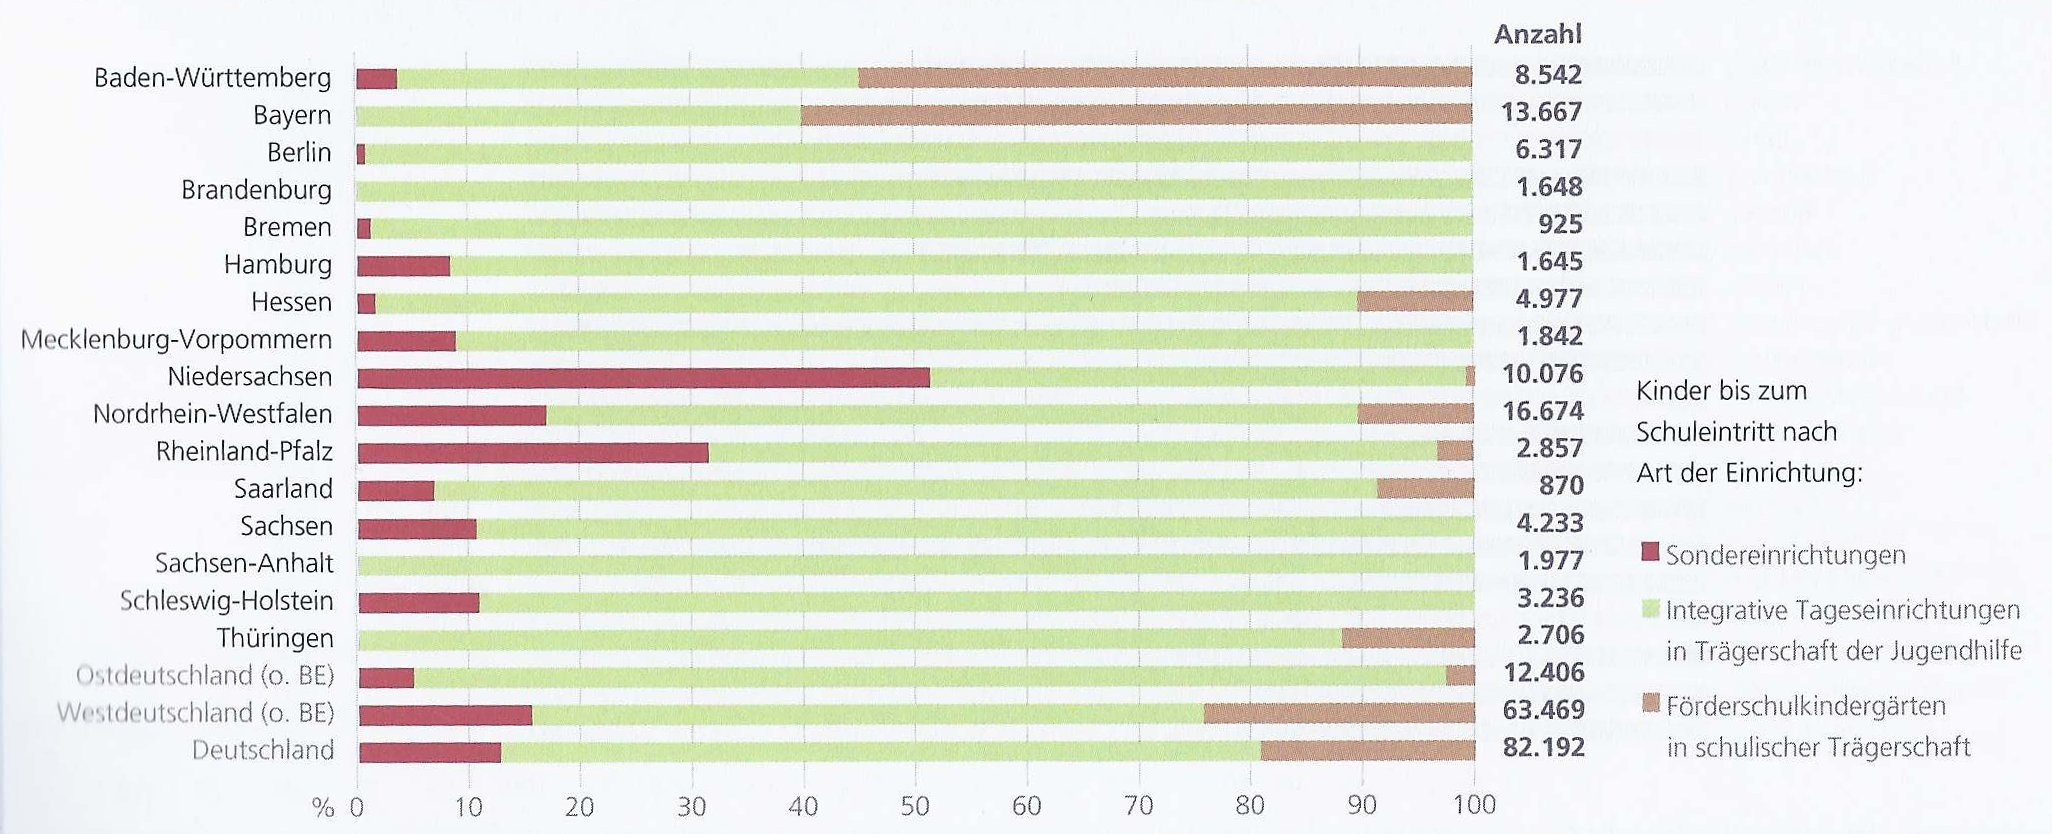
\includegraphics[width=0.95\textwidth]{bilder/bildungsbeteiligung}
  \caption{Bildunsbeteiligung von Kindern mit (drohender) Behinderung nach Art der Einrichtung. Stand: 01.03.2010. In: Bock-Famulla und Lange (2011, 13)}
  \label{bild:bildungsbeteiligung}
\end{figure}

\paragraph{Im Bildungsplan}
Nach Papke (2010) kann der Bildungsplan an sich als bedeutsamer Beitrag zur Inklusion verstanden werden, da mit dem Dokument vorgelegt wurde, was im schulischen Bereich gefordert wird: ein einheitlicher individualisierter Bildungsplan, der für alle Kinder gilt und ihre individuellen Bedürfnisse in den Blick nimmt. Welche Bedeutung ein solcher Bildungsplan für den Bereich der Kindertageseinrichtung hat, wird vor allem deutlich, wenn der Sektor Schule mit seinen unterschiedlichen Bildungsplänen für unterschiedliche Schultypen als Vergleich herangezogen wird. Worin besteht der Gewinn, dass im Bereich der Kindertagesbetreuung darauf verzichtet wurde? Papke schreibt, dass im Vorfeld Kindergruppen festgelegt werden müssten, für diese müsste ein 'gesundes Maß' an Bildungsinhalten und Anforderungen portioniert werden und aus diesen Anforderungen wiederum würden sich nach und nach pädagogische Erwartungen und Haltung formen. Im Bildungsplan für Kindertageseinrichtungen entfallen solcherart Trennungslinien und Kategorisierung im Sinne einer defizitorientierten Pädagogik. Ein grundsätzlich individualisierter und inklusiver Förderansatz ist damit formal umgesetzt. Trotz Kapitelüberschriften wie 'Vielfalt, Unterschiedlichkeit und Gemeinsamkeit' im baden-württembergischen oder 'Umgang mit individuellen Unterschieden' im hessischen Bildungsplan formuliert Nagel (2009, 19) jedoch den Bedarf, den positiven Umgang mit Unterschieden in den Plänen auszubauen. Viernickel und Schwarz (2009, 16) bestätigen die Diskrepanz zwischen den Inhalten der Bildungspläne, die von ihnen als „ehrgeizig formulierte Ansprüche an die frühkindliche Bildung“ bezeichnet werden und der gelebten Praxis in Kindertageseinrichtungen. Insbesondere das Qualitätsmerkmal 'Personalschlüssel' läuft den ehrgeizigen Ansprüchen zuwider und hemmt die Handlungsfähigkeit der pädagogischen Fachkräfte.

Gemeinsame Erziehung von Kindern mit und ohne Behinderung wird zahlenmäßig mit Abstand am weitesten in den Einrichtungen des Elementarbereichs umgesetzt (vgl. Kron 2002, Papke 2010, Sarimski 2011), die Unterschiede zwischen den Bundesländern sind nach Bock-Famulla und Lange (2011, 13) jedoch erheblich (vgl. Tabelle in Abbildung~\ref{bild:bildungsbeteiligung}). In Brandenburg und Sachsen-Anhalt besuchen alle Kinder integrative Einrichtungen. Dagegen ist der Anteil der Kinder, die in Sondereinrichtungen betreut werden, in Baden-Württemberg, Bayern und Niedersachsen am höchsten und liegt bei über 50\,\%. 

\section{Selbstverständnis des Kindergartens unter Berücksichtigung der Trägervielfalt}\label{sec:kitaSelbst}
Aus den vorangestellten Bezugspunkten und ihren Aufgabenbeschreibungen lässt sich laut Hugoth (2010, 30) das Selbstverständnis des Kindergartens ableiten. Seine Ausdifferenzierungen sollen vorab als Übersicht präsentiert werden:

Der Kindergarten als
\begin{enumerate}
\item erste Stufe des deutschen Bildungssystems,
\item Ergänzung und Unterstützung der Familie,
\item Dienstleister und Teil des Systems der unterstützenden Dienste,
\item Organ des Staates zur Erfüllung seines Wächteramtes und 
\item Ort für alle.
\end{enumerate}

Die inhaltlichen Schwerpunkte der Arbeit im Kindergarten werden nach Hugoth (2010, 19) maßgeblich durch den Träger beeinflusst. Die Einrichtungen weisen ein jeweils trägerspezifisches Profil auf, welches sich in der Auswahl des Personals, in der Organisationsform, im Erscheinungsbild nach außen, in der Schwerpunktsetzung der Arbeit und in der gelebten 'Philosophie' unterscheidet. Dadurch heben sich die Einrichtungen, vor allem die der freien Träger, zum Teil stark voneinander ab. Deutschland hat im Vergleich zu anderen europäischen Ländern die vielfältigste und bunteste Trägerlandschaft. 
Im SGB VIII~§~3 (vgl. Gastiger und Winkler 2009, 312) wird zwischen öffentlichen und freien Trägern unterschieden. Zu den öffentlichen gehören nach §~69 SBG~VIII (ebd., 341) die Landkreise und kreisfreien Städte und die kreisangehörigen Gemeinden. Hugoth (2010, 20) verweist darauf, dass zunehmend mehr Landesgesetze die institutionalisierte Kinderbetreuung in die Hände der Gemeinden vor Ort geben. 

Zu den freien Trägern zählen laut Hugoth: 
\begin{itemize}
\item die kirchlichen Wohlfahrtsverbände Caritas und Diakonie und die katholischen und evangelischen Kirchgemeinden, die mit über 50\,\%
Gesamtanteil (Stand: 2000) das größte Kontingent stellen, 
\item darüber hinaus die Wohlfahrtsverbände wie Arbeiterwohlfahrt, Rotes Kreuz, Paritätischer Wohlfahrtsverband mit ihren Unterorganisationen,
\item Elterninitiativen, Unternehmen und Betriebe sowie
\item gewerbliche Träger\footnote{Auch wenn gewerbliche Träger eigentlich zu den freien Trägern zählen, fallen dem Sprachgebrauch nach alle nicht-staatlichen und nicht-gewerblichen unter die freien Träger.}, zum Beispiel 'Little Giants'. Diese zählen zu den teuren, bilingualen Kindergärten und werden von Weiß (2010) als 'Parallelwelt' für Privilegierte bezeichnet\footnote{Die Homepage gibt weitere Einblicke in das Konzept von Little Giants: http://www.littlegiants.de}.      
\end{itemize}

Die Qualität einer Kindertageseinrichtung hängt nach Hugoth und Jansen (2005, 9 f.) im entscheidenden Maße vom Engagement ihres Trägers ab. Erfolg lässt sich danach bemessen, ob der Träger sein Profil zu schärfen in der Lage ist, indem er es an fachlichen, politischen und gegebenenfalls kirchlichen Anforderungen ausrichtet. Ein professionelles Profil begünstigt eine gute Ausgangsposition im Wettbewerb und dementsprechend berufliche Sicherheit. Die an den Trägerverbund gestellten Anforderungen sind sehr komplex und reichen von der wirtschaftlichen Steuerung und Zukunftssicherung der Einrichtung bis hin zu inhaltlichen Fragen. Dem Träger wie auch der Leitung obliegen eine übergeordnete Steuerungsfunktion. Der Einfluss des Träger auf das Selbstverständnis des Kindergartens kann als entsprechend groß bewertet werden, wenn dieser als „Förderer, Unterstützer und Initiator von Entwicklungen in den Einrichtungen“ (Rückert 2011, 13) verstanden wird. Seine Interessen bilden das übergeordnete Wertesystem der Einrichtung. Wenn sich die kirchlichen Träger, zu denen in der Regel die zahlenmäßig stark vertretenen Gemeinden vor Ort zählen, zu aktuellen sozialpolitischen oder bildungspolitischen Themen öffentlich äußern oder zukunftsweisende Entscheidungen treffen, sind diese nicht nur für einzelne Familien, sondern für die ganze Gesellschaft von nachhaltiger Bedeutung. Somit steht der Träger im Dienste der Gesellschaft. Hier sei als Beispiel die Caritas Kampagne 2011 benannt, in der Inklusion zum Jahresthema ernannt und mit folgendem Leitsatz präsentiert wurde: „Kein Mensch ist perfekt! Behinderte Menschen: Menschen wie du und ich!“ (Caritas 2011) Da die Kindergartenträger in eigener Verantwortung ihre Aufgaben beurteilen, hängt die Umsetzung von inklusiver Qualität im Kindergarten laut Rückert (2011, 133) davon ab,  ob die Träger sich ihrer Aufgaben und Verantwortungsbereiche in der gesamtgesellschaftlichen Tragweite bewusst sind und in Abhängigkeit dessen, wo sie in ihren Überlegungen stehen, entsprechende Schritte in Richtung inklusive Erziehungs- und Bildungsarbeit gehen.  
   
\subsection{Der Kindergarten als erste Stufe des deutschen Bildungssystems}
Liegle (2006, 6) schreibt, dass im Zuge der Etablierung des Kindergartens als erste Stufe des deutschen Bildungssystems Fragen in der Öffentlichkeit unterschiedlich diskutiert werden: Ist es die Aufgabe des Kindergartens auf das Lernen in der Schule vorzubereiten oder droht der Kindergarten in Folge dessen zu verschulen? Hugoth (2010, 32) fügt als weiteren Punkt in der Diskussion die Frage nach der Abschaffung der Elternbeiträge an. Die Elternbeiträge werden vom Träger der Einrichtung festgelegt. Befürworter verweisen auf den Schulbesuch, der ebenfalls ohne Beitragszahlung der Eltern auskommt. Kritiker benennen, dass das System Kindergarten dadurch vor allem für freie Träger nicht mehr bezahlbar sei, weil diese den Fehlbetrag aus dem Mangel der Elternbeiträge nicht kompensieren könnten und sich zurückziehen würden. Das birgt die Gefahr, dass die Vielfalt der Träger- und damit der Kindergartenlandschaft geschmälert und die Wahlfreiheit der Eltern gegebenenfalls unterlaufen werden würde. Dass solcherart Fragen öffentlich unterschiedlich diskutiert werden, beweist die Unterschiedlichkeit der Trägerinteressen, stellvertretend für eine pluralistische Gesellschaft. 

Sowohl im SGB VIII als auch im Bildungsplan wird die wechselseitige Zusammenarbeit von Kindergarten und Schule zur Gewährleistung eines guten Übergangs als wichtige Aufgabe formuliert. Nach Liegle (2006,~5~f.) sollen beide Bildungseinrichtungen aufeinander aufbauen, sodass Brüche beim Übergang von der einen zur nächsten Stufe vermieden werden und eine gewisse Kontinuität gewährleistet ist. Er beschreibt jedoch mit kritischem Blick die politische Tendenz in Deutschland, die Misere des Bildungssystems mit Hilfe einer gezielten Förderung auf die Schule beheben zu wollen.
Dass politische Maßnahmen als Folge des PISA-Schocks zu kurz greifen, die den Kindergarten als vorschulische Einrichtung umdeuten wollen, kann mit Hilfe von empirischen Untersuchungen gezeigt werden. Nach  Macon (2002) in Liegle (ebd.) konnte in einer breit angelegten Studie nachgewiesen werden, dass Kinder, die ein stark formalisiertes und strukturiertes Vorschulprogramm besucht hatten, signifikant schlechtere Noten im sechsten Schuljahr bekamen als die Vergleichsgruppe, die Vorschulprogramme mit Betonung auf selbstinitiierten und spielerischen Lernen besucht hatten. 
Laut Becker-Stoll (2009, 46) wird ein Kindergarten zu hinterfragen sein, der den Zusammenhang von Bindung und Bildung missachtet und Lerninhalte statt das Kind und seine Selbsttätigkeit ins Zentrum stellt. Sie argumentiert, dass zu den psychischen Grundbedürfnissen eines Kindes neben Autonomie und Kompetenz auch Bindung gehört. Bindung steht für das Bedürfnis, enge zwischenmenschliche Beziehungen einzugehen und sich innerhalb dieser Interaktion als liebenswert und liebesfähig zu erleben. 
 
Nach Papke (2010) besteht aus der Perspektive der Inklusion die Gefahr, dass manche Bildungsbereiche, die im Bildungsplan benannt werden, nicht für alle Kinder als gleichermaßen wichtig angesehen werden, zum Beispiel Naturwissenschaften und Mathematik. Daran schließt sich die Frage an, gesetzt dem Fall die Fachkräfte in den Einrichtungen sind davon überzeugt, dass alle Kinder in Bezug auf die empfohlenen Bildungsbereiche gleichermaßen anzusprechen sind, was muss bei der Gestaltung dieser Bildungsbereiche berücksichtigt werden, damit diese für alle Kinder interessant und individuell nutzbringend sind? Nur durch eine solche angeregte Auseinandersetzung kann „einem Denken in unterschiedlichen 'Bildungsgruppen' [vorgebeugt werden]“ (Papke 2010).
 
\subsection{Der Kindergarten als Ergänzung der Familie}
Laut Bock-Famulla und Lange (2011, 41) ist die Bildungspartnerschaft zwischen Kindergarten und Eltern von zentraler Bedeutung für die optimale Entwicklung des Kindes im Kindergarten. Jeske (1997, 10) bestätigt ebenfalls, dass, wenn zwischen beiden Lebenswelten positive enge Verbindungen statt starker Gegensätze bestehen, sich dies positiv auf die Entwicklung auswirken würde. Nagel (2009, 204) verweist auf verschiedene Studien, in denen die Interaktionswirkungen zwischen familiärer und außerfamiliärer Betreuung untersucht wird. Die bisherigen Ergebnisse zeigen, dass Entwicklungs- und Bildungschancen vor allem bei ’bildungsfernen’ Familien durch ergänzende Betreuung unterstützt werden können, die Unterstützung jedoch effizienter ist, umso aktiver die Familie selbst unterstützend wirken kann. Der Grund hierfür ist laut Albers (2011, 116) in dem Einfluss der Familie auf die kindliche Entwicklung zu sehen, der als etwa doppelt so hoch gilt wie der Einfluss institutionalisierter Betreuung. Es kann davon ausgegangen werden, dass beide Bereiche sich gegenseitig beeinflussen und eine gute Kooperation und Abstimmung mit den Eltern deshalb betont werden muss. 

Konkrete Vorgaben zur Elternbeteiligung werden laut Schlecht, Förster, Wellner und Mörth (2008, 44) in den Bildungsplänen gemacht. Bereits im Zusammenhang mit der Aufnahme des Kindes wird als wichtig angesehen, dass Eltern die Möglichkeit gegeben wird, gemeinsam mit ihrem Kind in der Gruppe zu hospitieren und in Austausch mit der Erzieherin zu treten, um mit der Einrichtung, ihrem Konzept sowie der Gruppe vertraut zu werden. Zur Aufgabe der Erzieherin gehört es familiäre, kulturelle und religiöse Besonderheiten des Kindes zu berücksichtigen und diese in den Alltag einzubeziehen. 'Bildungspartnerschaft' mit den Eltern kann durch regelmäßige Elternabende, jährliche Entwicklungsgespräche und allgemeinen Austausch über die Aktivitäten des Kindes erfolgen. Wünschenswert ist auch, dass die Eltern die Möglichkeit bekommen, ihre Interessen in die pädagogische Arbeit einzubringen und bei Planungs\- und Entscheidungsprozessen berücksichtigt werden.

\subsection{Der Kindergarten als Dienstleister}
Nach Hugoth (2010, 34 f.) hat sich in den letzten Jahren bedingt durch eine kritischere Erwartungshaltung von Seiten der Eltern, des Trägers aber auch der Behörden im Bereich der Kinder- und Jugendhilfe der Kindergarten zu einem Dienstleister entwickelt. An selbigen werden  Fragen gerichtet, ob er in Anbetracht dessen, was er leistet, das wert ist, was in ihn investiert wird und ob die erbrachten Leistungen den Bedürfnissen der Kinder und Familien entsprechen. Zudem verstehen sich Eltern nicht mehr als 'Laien', die ihre Kinder von 'Profis' betreuen lassen, sondern vielmehr als Kunden, die ausgewiesene Dienstleistungen erwarten und wird ihren Erwartungen nicht entsprochen, sich nach anderen Kindergartenplätzen umschauen. Er (2010, 35) verweist auf den Aspekt, dass in vielen Kommunen ein Konkurrenzdruck durch ein Überangebot an Kindergartenplätzen und eine schwindende Kinderzahl entsteht. Das zwingt die Einrichtung ihre Qualität unter Beweis zu stellen, um konkurrenzfähig zu bleiben. 
Kritisch merkt er (2010, 36 f.) jedoch an, dass eine Einrichtung, die in Leistungskategorien denkt und stets die Bedarfe des Kunden, also der Eltern, im Blick hat, an ihre Grenzen stoßen wird, da sie auch gesetzlichen Vorgaben, dem vom Träger vorgegebenen Profil, fachlichem Wissen sowie beruflicher Erfahrung verpflichtet ist. Hierbei können Elterninteressen und eigene Vorstellungen, was das 'Beste' für das Kind ist kollidieren. Fritz und Hugoth (2010, 28) empfehlen deshalb von einer „Dienstleistungsorientierung“ statt einem „Dienstleistungsunternehmen“ zu sprechen. Eine reine Orientierung an Kundenzufriedenheit ist der Qualität der Kindertageseinrichtung nicht förderlich. 

\subsection{Der Kindergarten als Organ des Staates zur Erfüllung des Wächteramtes}
Die Aufgabe des Wächteramtes ist gesetzlich klar geregelt. Der Träger ist in der Pflicht diesen Auftrag zu erfüllen, Spielraum bei der Umsetzung gibt es in diesem Fall nicht.
 
Hugoth (2010, 32) verweist darauf, dass, um die Kooperation und Vernetzung der Hilfesysteme zu verbessern, die Kindertagesstätten in das staatliche Wächteramt einbezogen wurden, welches nun zu ihrem Betreuungsauftrag gehört. Laut ihm (2010, 33) kann die Umsetzung eines so definierten Betreuungsauftrag zu einem Interrollenkonflikt der Erzieherin führen. Die unterschiedlichen Rollen, in denen sie sich befindet, einerseits Wächter und Anwalt des Kindes, andererseits Partner der Eltern, können im Einzelfall zuwider laufen. Transparenz des Kindergartens gegenüber den Eltern sei deshalb geboten, das heißt konkrete Interessen, Inhalte, Arbeitsweisen und normative Grundlagen des Kindergartens sollten klar definiert und mit den Eltern kommuniziert werden.

\subsection{Der Kindergarten als Ort für alle}\label{OrtFuerAlle}
Statistiken zeigen, dass nahezu jedes Kind in Deutschland einen Kindergartenplatz in Anspruch nimmt, weshalb laut Kron (2010, 32 f.) davon ausgegangen werden kann, dass die Heterogenität\footnote{Nach Prengel und Heinze (2012) bedeutet 'heterogen' verschieden, anders, plural. Heterogenität stellt ein Verhältnis von Verschiedenen dar, die einander nicht untergeordnet, sondern gleichgestellt sind. Im vorliegenden Kontext bezieht sich der Begriff auf die zu respektierenden Differenzen zwischen einzelnen Kindern, also auf ihre individuelle Einzigartigkeit innerhalb der Gruppe.}
der Kindergartengruppe die gesellschaftliche Vielfalt repräsentiert, davon ausgenommen jedoch die Zahl der in Sondereinrichtungen betreuten Kinder. Die europäische multikulturelle Gesellschaft zeichnet sich durch immer komplexer werdende Differenzen und eine wachsende gesellschaftliche Vielfalt aus, in der traditionelle Unterscheidungsmerkmale verschwimmen. Gründe hierfür sieht Speck-Hamdan (2011, 16) in der Migrationsbewegung und in Individualisierungsprozessen. Der Kindergarten wird somit zum Spiegel dieser Vielfalt – „die Welt trifft sich im Kindergarten“\footnote{Buchtitel von Oberhuemer, Soltendieck und Ulrich, 2001}.
 
Um das Spektrum an Unterschieden überschaubar zu machen, werden eine Reihe von Kategorien angelegt. Im derzeitigen Interesse der Sozialwissenschaften liegen laut Albers (2011, 37) vor allem die Kategorien Migration, Behinderung, sozialer Hintergrund und Geschlechtszugehörigkeit.
Wenn jedoch nur ein Unterscheidungsmerkmal untersucht wird, kann es nach Speck-Hamdan (2011, 16) zu Verkürzungen kommen, weil sich Differenzlinien überschneiden und die Individualität des Menschen gerade dadurch bestimmt wird, dass er mit mehreren Facetten zu beschreiben ist. Deshalb sind die in den Sozialwissenschaften in den Vordergrund gestellten Facetten bei weitem nicht alle, anhand derer Kinder voneinander unterschieden werden können. Mögliche weitere Kategorien zur Wahrnehmung der Differenzen in einer Kindergartengruppe bestehen hinsichtlich Alter, kultureller Herkunft, Sprache, Glaubensrichtung, Eltern, Geschwister, Familienkultur und Sozialisation, Qualität ihrer Bindungserfahrungen, Bildungsbiografie, Lernumfeld, ökonomischer Lebenslage, Entwicklungsverlauf sowie bisheriger Erfahrungen in gleichaltrigen Gruppen. 

Eine Bestandsaufnahme hinsichtlich der Merkmale Migrationshintergrund, soziale Benachteiligung und Behinderung beziehungsweise Entwicklungserschwernisse schließt sich an.

Laut Roth und Terhart (2009, 8) hat im Jahre 2008 etwa jedes vierte Kindergartenkind einen Migrationshintergrund, das heißt, es selbst oder mindestens eines seiner Elternteile oder auch eines seiner Großelternteile ist seit der Nachkriegszeit in Deutschland eingewandert. Hierbei wird ein großer Ost-West-Unterschied deutlich. In den westdeutschen Bundesländern haben 29\,\% der über Dreijährigen einen Migrationshintergrund, in den ostdeutschen Bundesländern lediglich 6\,\%. Von allen Migrantenkindern besucht nahezu jedes dritte Kind eine Gruppe, die sich wiederum zu mindestens 50\,\% aus Kindern mit Migrationshintergrund zusammensetzt. Bei Kindern mit Migrationshintergrund handelt es sich ebenfalls um eine sehr heterogene Gruppe, über die nur sehr schwer allgemeine Aussagen getroffen werden können. Ein verbindender Aspekt ist die häufige Zwei- oder Mehrsprachigkeit. Unterschiede machen sich fest an den Herkunftsländern, der ethnischen Zugehörigkeit, der Aufenthaltsdauer, dem rechtlichen Status und den Beweggründen der Eltern nach Deutschland zu kommen. Der kulturelle Hintergrund kann nach Albers (2011, 38) nicht ohne Bezugnahme auf Faktoren wie Geschlecht, sozialer Status, Einkommen, Bildungshintergrund, Religion und Alter gesehen werden. 

Im Sinne von Inklusion ist Migration als ein Merkmal unter vielen zu verstehen, wodurch an den Lebenswelten des Kindes angesetzt und somit ein individuell-biografischer Zugang zum Kind ermöglicht sowie Diskriminierung vermieden werden kann. Das folgende Beispiel verdeutlicht diesen Zugang: Ali ist ein Junge, ein Kind, der Bruder von zwei Schwestern, begeisterter Fußballspieler, Türke (vgl. Fachforum 2012 ??).    
 
Was sagt ein Migrationshintergrund noch über das Kind aus? Laut Roth und Terhart (2009, 77~f.) steht der Migrationshintergrund in Korrelation zu Armutsverhältnissen. 
Mittels der Längsschnittstudie zur Kinderarmut in Deutschland vom Institut für Sozialarbeit und Sozialpädagogik (1997 - 2005) wurde herausgefunden, dass bei der Gruppe der Vorschulkinder die Armutsquote bei Kindern mit Migrationshintergrund mit über 40\,\% mehr als doppelt so hoch ist wie bei den Kindern mit deutschem Pass. Gründe für Einkommensarmut der Familien sind vor allem in Zugangsbarrieren zum Ausbildungs- und Arbeitsmarkt und einem häufig niedrigeren Bildungsniveau der Eltern zu suchen. 
Laut Weiß (2010) wächst auf der einen Seite der Wohlstand, zwei Drittel der Kinder in Deutschland geht es materiell so gut wie keiner Generation vorher, auf der anderen Seite wächst die Gruppe der sozial Ausgegrenzten, 2~bis~2,5 Millionen Kinder und Jugendliche leben bis zum 18. Lebensjahr von staatlicher Unterstützung. 
Forschungen haben ergeben, dass Armut an sich noch kein direktes Risiko für die kindliche Entwicklung darstellt, jedoch die Wahrscheinlichkeit für Entwicklungsgefährdungen, bedingt durch komplexe Unterversorgung oder ein unzureichendes oder schädigendes Erziehungsverhalten seitens der Bezugspersonen, erhöht ist. 
Nach Weiß (2000, 52 f.) hängt das Entwicklungsrisiko vom Ausmaß der Armut, sowohl von ihrer Dauer als auch von ihrer Komplexität und Intensität, und zudem von den Bewältigungsstrategien der betroffenen Familien ab. Bei chronischer Armut besteht ein wesentlich größeres Risiko als bei kürzeren Armutsperioden, da individuelle Handlungsspielräume in zentralen Lebensbereichen eingeengt werden oder verloren gehen.
Vor allem bei chronischer Armut werden laut ihm die betroffenen Menschen nicht selten von der Erwerbsgesellschaft ausgegrenzt und fühlen sich in Folge dessen überflüssig, nutzlos und nicht gebraucht, wodurch Zukunftsperspektiven schwinden und gehäuft Selbstentwertung und Verunsicherung auftreten. Wenn Kinder in eine solche familiäre Situation hinein geboren werden, dann ist das Risiko erhöht, dass sie auf Eltern treffen, die nicht die Kraft haben den Aufgaben der Pflege und Erziehung hinreichend nachzukommen und die intuitive und empathische Kompetenzen vermissen lassen, da sie bedrängt von hoher existenzieller Unsicherheit in ihren Alltagsproblemen gefangen sind.   
Grundsätzlich besteht „ein plausibler und auch empirisch nachgewiesener Zusammenhang zwischen soziökonomischen und psychosozialen Belastungssituationen sowie der kindlichen Entwicklungsgefährdung bis hin zu manifesten Behinderungen“ (Weiß 2000, 51).

Biedinger (2009, 197) hat die Folgen von Einkommensarmut auf die kognitive Entwicklung, das Sozialverhalten und den Wortschatzumfang von 3 bis 4-jährigen Kindern untersucht. Die Ergebnisse zeigen, dass der Einfluss der Armut auf die kindliche Entwicklung und den Wortschatz, jedoch nicht auf das Sozialverhalten signifikant ist und selbst unter Kontrolle der Bildung der Bezugsperson bestehen bleibt. Es konnte gezeigt werden, dass der häusliche Lern- und Erfahrungsspielraum entscheidenden Einfluss auf die Entwicklung nimmt und bei Familien in Armut als ebenfalls verarmt betrachtet werden kann, genauso wie ihre Entfaltungs- und Bildungsmöglichkeiten und die Förderung ihrer individuellen Neigungen und Fähigkeiten.

Kinder in Armut sind eine Herausforderung für inklusive Erziehungs- und Bildungsarbeit, weil sie einerseits in ihrer Verschiedenheit zu anderen gesehen und anerkannt werden müssen, aber bloße Anerkennung keine Antwort auf eine „wachsende gesellschaftliche Ungleichheit und ihre Exklusion fördernden Folgen“ (Weiß 2010) ist. Inklusion verfolgt das Ziel sozialer Gerechtigkeit, das heißt, dass dem Bildungssystem eine kompensatorische Funktion zukommt.       
 
Da Behinderung nach Albers (2011, 38) aus der Wechselwirkung von funktionaler Beeinträchtigung im Zusammenwirken mit sozialen Faktoren entsteht, ist auch hier ein mehrdimensionaler Blick erforderlich. Kinder mit Behinderung sind im Kindergarten zunächst einmal Kinder mit bestimmten Voraussetzungen, zum Beispiel Hörverlust, Sehbeeinträchtigung oder Down-Syndrom, die sich erschwerend auf ihre Entwicklung und ihr Lernen auswirken. Jeder Diagnose liegt eine Spannweite von leichter bis schwerer Ausprägung zugrunde. Kinder mit Down-Syndrom zum Beispiel haben eine Intelligenzminderung und trotzdem gibt es Kinder unter ihnen, die das Abitur absolvieren und wiederum andere, die kaum beschulbar sind. Zudem können auch mehrere dieser bestimmten Voraussetzungen bei einem Kind vorliegen, was die Gruppe der Kinder mit Behinderung insgesamt zu einer sehr heterogenen Gruppe macht. Sarimski (2012, 10) gibt die Prävalenz für unterschiedliche Formen von Behinderung mit insgesamt drei bis vier Prozent an. Darunter zählt er Kinder mit einer Seh- oder Hörschädigung, Körperbehinderung, Spracherwerbs\-störung, Lern- oder geistigen Behinderung oder mit Autismusspektrumsstörung. 
Eine sehr viel größere Gruppe bilden Kinder mit Entwicklungsrückständen ohne erkennbare biologische Beeinträchtigung, Teilleistungsstörungen, Verhaltensauffälligkeiten oder in außergewöhnlichen Belastungssituationen, zum Beispiel Kinder psychisch kranker oder suchtkranker Eltern. Nach Klein (2010, 12) zeigt insgesamt jedes fünfte Kind eine solche Entwicklungsproblematik. 

Zusammenfassend kann nach Kron (2010, 32 f.) festgehalten werden, dass Kinder in Deutschland unter sehr unterschiedlichen Bedingungen aufwachsen, sodass Heterogenität eine soziale Tatsache darstellt. 
Gemeinsam ist allen Kindern, dass sie Kinder sind und dass sie alle einzigartige Bedürfnisse haben. 
Da die Unterschiedlichkeit der Kinder als reale Ausgangslage anerkannt werden muss, gilt es laut Sarimski (2012, 11) pädagogische Lösungen zu entwickeln, die dieser Vielfalt gerecht werden. Das fokussierte Ziel muss demzufolge lauten, ausnahmslos alle Kinder in gleichermaßen guter Qualität betreuen, erziehen und bilden zu wollen.  

\section{Qualitätsmanagement in Kindertageseinrichtungen}

Laut Esch, Klaudy, Micheel und Stöbe-Blossey (2006, 9) ging die Bildungsdebatte Anfang der 90er Jahre Hand in Hand mit der nationalen und internationalen Diskussion über Qualitätsfragen im Elementarbereich, verbunden mit erhöhten Erwartungen an den Kindergarten, was dieser zu leisten habe und wie dieser beschaffen sein sollte. Wie bereits erwähnt sind die Träger der Kindertagesstätten seit der Erneuerung und Erweiterung des Kinder- und Jugendhilfegesetzes (§§~22 bis 24a SBG VIII) zur Qualitätsentwicklung verpflichtet. Eine steigende Qualität soll unter anderem Antwort auf bildungs- und sozialpolitische Herausforderungen geben, wie den erhöhten Anteil an Kindern mit Migrationshintergrund in Kindergartengruppen.
Bemühungen, Qualitätsmerkmale festzulegen und qualitätssichernde Maßnahmen zu etablieren, erfolgten laut Hugoth (2010, 30 f.) zum Beispiel durch die Implementierung der Bildungspläne oder die 1999 vom Bundesministerium für Familie, Frauen, Senioren und Jugend ins Leben gerufene \emph{Nationale Qualitätsinitiative im System der Tageseinrichtungen für Kinder} (NQI). Die aktuellste Antwort auf die Qualitätsfrage -- erste Ergebnisse liegen seit 2012 vor -- ist die \emph{Nationale Untersuchung zur Bildung, Betreuung und Erziehung in der frühen Kindheit} (NUBBEK). Durch die gemeinsame Anstrengung von Tietze, Becker-Stoll, Bensel, Eckhardt, Haug-Schnabel, Kalicki, Keller und Leyendecker (2012, 4) hat sich die  NUBBEK-Studie zum Ziel gesetzt auf hinreichend großer Datenbasis die Qualität in unserem Früherziehungssystem sowohl bezogen auf die Betreuungsqualität in der Familie als auch im institutionellen Setting zu untersuchen. 
  
\subsection{Pädagogische Qualität und ihre Dimensionen}

Tietze (2004, 406) definiert den Qualitätsbegriffs sehr allgemein: Mit Qualität wird die Beschaffenheit einer Dienstleistung bezeichnet und durch eine Reihe charakteristischer und überprüfbarer Eigenschaften näher beschrieben, welche für den Nutzer der Dienstleistung von Bedeutung sind. In dieser Begriffsbestimmung können in Bezug auf das Untersuchungsfeld Kindergarten drei Variablen näher bestimmt werden:

\begin{enumerate}
\item Die Dienstleistung als eine pädagogische bezieht sich auf die Trias Betreuung, Bildung und Erziehung.
\item Genutzt wird diese Dienstleistung von den Eltern, den Kindern und den Erzieherinnen.
\item Die Dimensionierung der Eigenschaften in Strukur-, Orientierungs- und Prozessqualität wird laut  Tietze (2004, 407) als hilfreich erachtet. Zudem kann laut Behr (2009, 67) die Ergebnisqualität als weiteres Unterscheidungskonstrukt festgelegt werden.
\end{enumerate}

Laut Ahnert (2011, 153 f.) stellt das Messen von Qualität institutionalisierter Betreuung ein schwieriges Unterfangen dar, da von Seiten der betroffenen Nutzer unterschiedliche Qualitätsvorstellungen zu erwarten sind beziehungsweise die Nutzer dieselben Eigenschaften möglicherweise unterschiedlich bewerten. Aus Elternsicht würde sich die Qualität der Einrichtung beispielsweise an Wohnortnähe und adäquaten Betreuungszeiten -- Merkmale, die mit ihrem Beruf gut vereinbar sind -- bemessen. Das Qualitätsmerkmal 'verlängerte Öffnungszeiten' würde aber aus der Perspektive der Erzieherin bedeuten, einen Arbeitsplatz mit Schichtbetrieb und daraus resultierend familienunfreundliche Arbeitszeiten vorzufinden.  
Um Klarheit in die Qualitätsdebatte zu bringen, wurde von der National Association for Education of Young Children (NAEYC) schon vor längerer Zeit das Kind ins Zentrum der Debatte gestellt. Somit gilt, wenn nach Tietze (2004, 407) von pädagogischer Qualität gesprochen wird, dann wird ein konkreter Bezug zur kindlichen Entwicklung vorausgesetzt. Pädagogische Qualität ist nur dann gegeben, „wenn diese das körperliche, emotionale, soziale, intellektuelle Wohl sowie die gegenwärtigen und zukünftigen Entwicklungen der Kinder in diesen Bereichen fördert und die Familien in ihrer Betreuungs- und Erziehungsaufgabe unterstützt“ (Tietze 2004, 407). Um pädagogische Qualität zu bestimmen, müssen vorab Qualitätsindikatoren in Bezug auf einen guten Kindergarten unter Perspektive des Kindes und seiner Entwicklungsförderung entwickelt werden. Die Qualität als Ergebnis misst sich dann daran, inwieweit diese Festlegungen in der Praxis der Einrichtung umgesetzt werden konnten. 

Kritisch merken Honig et al. (2004, 13 f.) an, dass die dominierende frühpädagogische Qualitätsdebatte, die wie selbstverständlich auf das Kind und seine Entwicklung sowie auf den Handlungsraum der einzelnen Einrichtung bezogen ist, eine Verengung darstellt, weil wichtige Aspekte unberücksichtigt bleiben. Kindergärten sind 'soziale Räume' und als solche in komplexe gesellschaftliche Funktionszusammenhänge und kulturelle Kontexte eingebettet. „Daher sind die Maßstäbe für einen guten Kindergarten nicht nur vielfältig, sondern unvermeidlich strittig; bei genauem Hinsehen weisen sie sogar eine dilemmatische Struktur auf, weil das System der Tageseinrichtungen für Kinder in ein Netz heterogener generalisierter Erwartungshorizonte eingebunden ist. Kindergärten sind entsprechend Schauplatz von Auseinandersetzungen um unterschiedliche Interessen, die mit ungleichen Einflusschancen ausgestattet sind. [...] Kindergärten vermögen ihre Güte also nicht autonom zu bestimmen“, sondern müssen die Differenzen immer wieder austarieren. 
Nach Meinung der Autoren sollte der Qualitätsdiskurs von der Frage bestimmt werden, wie sich die unterschiedlichen Erwartungen miteinander vereinbaren lassen.

Die Weiterentwicklung der pädagogischen Arbeit und die Qualitätssicherung ist laut Tietze, Dittrich, Grenner, Groot-Wilken, Sommerfeld und Viernickel (2004, 16 f.) in der Regel Aufgabe der Leitung. Davon abweichend können Qualitätsbeauftragte als Koordinatoren vom Träger gestellt werden oder aber die Leitung überträgt diese Aufgabe einer Fachkraft aus dem Team. 
Der Gewinn in der Anwendung von Qualitätsmanagementverfahren für die pädagogische Fachkraft liegt nach Volkert (2008, 75) in einem  wachsenden professionellen Selbstverständnis, das entsteht, wenn Prozesse, um sie zu verbessern, differenziert und reflektiert betrachten werden.

Nach Behr (2009, 14) impliziert pädagogische Qualität im Bezug auf Kinder mit besonderen Bedürfnissen stets die Dimension der Inklusion, da durch die Behinderung zugleich die Aufgabe der Einbeziehung und Partizipation gestellt ist. 

In den folgenden Kapiteln werden die vier Qualitätsdimensionen vorgestellt und durch Beispiele bestehender Qualitätsstandards vor allem im Hinblick auf Inklusion ergänzt.

\subsection{Strukturqualität}
\label{subsec:Strukturquali}
Laut Tietze (2004, 407) werden unter Strukturqualität Aspekte zusammengefasst, die situationsunabhängig, zeitlich stabil und politisch regulierbar sind. Solche strukturellen Rahmenbedingungen können wiederum unterschieden werden in einerseits der Einrichtung zur Verfügung stehende materielle Ressourcen und andererseits personelle Ressourcen. Unter materiellen Ressourcen werden die vorhandenen Räume und deren Ausstattung, die Finanzierung des Personals, der Betreuungsschlüssel, die Gruppengröße und die Gruppen- und Personalstruktur sowie die vorgesehenen Zeiten für mittelbare pädagogische Arbeit\footnote{ Mittelbare pädagogische Arbeit umfasst alle Aufgaben, die zusätzlich zu der direkten Arbeit mit den Kindern bestehen, zum Beispiel Elternarbeit, regelmäßige Dokumentation über Bildungs- und Entwicklungsförderung der Kinder oder Qualitätsentwicklung.} zusammengefasst, unter personelle Ressourcen zählt die Qualifikation der Fachkräfte, festgelegt durch Curriculum und Standards in der Erzieherinnen-Ausbildung. 

Nach Viernickel und Schwarz (2009, 15) werden die Ausbildung, Qualifikation und Bezahlung der pädagogischen Fachkräfte sowie der Betreuungsschlüsse und die Gruppengröße als zentrale strukturelle Rahmengrößen eingestuft, weil bei ihnen ein bedeutsamer Zusammenhang zur kindlichen Entwicklung und zu Aspekten der Prozessqualität nachgewiesen werden konnte. 
Hierfür ist der Betreuungsschlüssel ein geeignetes Beispiel. Die Expertise von Viernickel und Schwarz zur Bestimmung des Betreuungsschlüssels zeigt, je günstiger die Fachkraft-Kind-Relation ausfällt, desto positiver gestaltet sich die Prozessqualität, das heißt die pädagogischen Interaktionen, die bildungsanregenden Impulse, das Wohlbefinden und letztlich die Entwicklung der Kinder. Der Schwellenwert für drei bis sechsjährige, bei dessen Unterschreitung das Wohlbefinden der Kinder gefährdet ist, liegt bei circa eine Fachkraft auf acht Kinder. Die Ergebnisse dieser Expertise zeigen, dass die notwendigen Standards bei der Mehrzahl der Bundesländer nicht erreicht werden, weshalb die Bildungsansprüche, die in den Bildungsplänen benannt werden, schwer umzusetzen sind.

Qualitätsstandards in Bezug auf Kinder mit besonderen Bedürfnissen können laut Sarimski (2012, 145~f.) durch die Elternbefragung von Kobelt Neuhaus (2001) und die Befragung der pädagogischen Fachkräfte durch Dichans (1990) gewonnen werden:
 
\begin{itemize}
\item Aus Elternsicht: Gruppenstärke von nicht mehr als 18 Kindern, davon höchstens ein bis zwei Kinder mit Behinderung und zwei Fachkräfte 
beziehungsweise 
aus der Sicht der Erzieherinnen: Gruppenstärke von maximal 15 Kindern bei nicht mehr als einem Drittel Kindern mit Behinderung und drei Mitarbeitern, davon mindestens zwei Fachkräfte
\item barrierefreie Zugangsmöglichkeiten und entsprechende Ausstattung mit Materialien, die auf die spezifischen Bedürfnisse der Kinder zugeschnittenen sind
\item ausreichend Zeit, in der die Erzieherinnen von der Betreuung der Kinder freigestellt sind, um sich mit heilpädagogischen Fragen innerhalb und außerhalb des Teams zu befassen, Angebote sowie spezielle Fördermaßnahmen differenziert zu planen und intensive Beratung durch Fachdienste wahrzunehmen
\item Fortbildungsmöglichkeiten
\end{itemize}

\subsection{Orientierungsqualität}
Nach Tietze (2004, 411) erfordert ein entwicklungsfördernder Umgang mit dem Kind hohe formale und berufsbezogene Qualifikation. Eng im Zusammenhang mit der Ausbildungsqualität der Erzieherinnen steht die Orientierungsqualität. Diese umfasst laut ihm (2004, 407 f.) pädagogische Vorstellungen, Werte und Überzeugungen der Erzieherin. Welches Bild sie vom Kind, aber auch von den Eltern hat, wird ihre pädagogische Arbeit maßgeblich bestimmen. Für gelingende inklusive Bildungsprozesse ist eine ressourcenorientierte Haltung als Grundvoraussetzung anzusehen. Haltungen und Orientierungen werden in der Ausbildung erworben und in Fortbildungen vertieft, sind aber auch von der Persönlichkeit abhängig. 
Da die Empathiefähigkeit der Erzieherin Voraussetzung für eine sichere Bindungsbeziehung zum Kind ist, sehen Haderlein und Sell (2007, 24) die Notwendigkeit, die Frage nach der Persönlichkeit offen zu stellen. Denn, „nicht jeder Mensch ist in der Lage im Prozess der Praxis der Betreuung, Erziehung und Bildung von Kindern aus seiner Person selbst heraus eine hohe Qualität zu entfalten, auch und nicht selten trotz eines hohen Reflexionsgrades auf theoretischem Niveau“ (Haderlein und Sell 2007, 24). Anders als die Merkmale der Strukturqualität sind die Rahmengrößen der Orientierungsqualität nicht direkt politisch steuerbar, werden jedoch ebenso als zeitlich stabil angesehen. Oft werden übergeordnete Werte auch vom Träger vorgegeben. Sie werden aber auch von den Mitarbeiterinnen erarbeitet und der Konzeption der Einrichtung unter Beachtung vorhandener Rahmenrichtlinien zugrunde gelegt, sodass eine Verständigungsgrundlage nach innen und außen geschaffen wird. 

\subsection{Prozessqualität}\label{Prozessqualität}
Zur Prozessqualität zählt „all das, was den konkreten Erfahrungs- und Erlebnisraum des Kindes in der Einrichtung unmittelbar gestaltet und beeinflusst“ (Tietze 2001, 7). Prozessqualität bezieht sich auf den Kindergartenalltag mit seinen Interaktionen und Erfahrungen, die das Kind innerhalb seiner sozialen und räumlichen Umwelt macht. Die Prozessqualität wird als dynamisches Konstrukt bezeichnet, da sie situationsabhängig ist. Die Ergebnisse der NUBBEK-Studie herausgegeben von Tietze et al. (2012, 8) weisen im Bereich der Prozessqualität erhöhte Werte auf, wenn keine Altersmischung vorliegt und wenn offene, das heißt gruppenübergreifende Arbeit stattfindet. Es zeigen sich niedrigere Werte, je höher der Anteil an Kindern mit Migrationshintergrund ist. Weiterhin zeigt sich, dass die Prozessqualität entscheidend von den Persönlichkeitsmerkmalen der Erzieherin bestimmt wird, insbesondere ihrer Zufriedenheit. Hierin drückt sich die Abhängigkeit der Prozessqualität von Rahmenbedingungen der Struktur- und Orientierungsqualität aus.   

\subsection{Ergebnisqualität}
Die Ergebnisqualität ist vor allem für die Inklusionsperspektive relevant. Nach Behr (2009, 67) werden unter Ergebnisqualität  wahrnehmbare beziehungsweise messbare Auswirkungen einer Maßnahme verstanden, sodass gezeigt werden kann, ob durch spezifische Maßnahmen Entwicklungsfortschritte bei Kindern mit Entwicklungsgefährdungen erreicht werden können. Für die Beantwortung dieser Fragen können entwicklungsdiagnostische Testverfahren eingesetzt werden.



\chapter{Inklusion im Kindergarten}

\section{Warum Inklusion?}
\label{sec:Why}
Es folgen eine Reihe ausgewählter Begründungen, die zeigen, welchen Nutzen der Kindergarten verspricht, dessen Selbstverständnis es ist keine Türen der Ausgrenzung zu haben und inklusive Erziehungs- und Bildungsarbeit zu leisten. Die Auswahl der Argumente erhebt keinen Anspruch auf Vollständigkeit.

\subsection{Gemeinsame Erziehung und Bildung ist ein Menschenrecht}
\label{sec:BRK}
Es ist nicht nur von Behindertenverbänden, sondern darüber hinaus von der UN-Behindertenrechtskonvention gefordert und politisch gewollt, dass sich das Leben von Menschen mit Behinderungen nicht in Sondersystemen, sondern so weit wie möglich innerhalb der allgemeinen Lebenswelt abspielt. Wie auch die Kinderrechtskonvention ist die \emph{„UN-Behindertenkonvention über die Rechte von Menschen mit Behinderung“} laut Albers (2011, 26 f.) ein völkerrechtliches Abkommen. Die Mitgliedsstaaten verpflichten sich, indem sie den Völkerrechtsvertrag unterzeichnen, die darin getroffenen Bestimmungen in ihr geltendes Rechtssystem umzusetzen. Die Konvention wurde im Dezember 2006 von der Generalversammlung der vereinten Nationen verabschiedet. Im März des Folgejahres wurde sie von Deutschland unterzeichnet und im Dezember 2008 vom Deutschen Bundestag und Bundesrat ratifiziert. In deutsches Recht ist selbige seit 24.03.2009 umzusetzen, das heißt konkret, dass deutsche Gesetze überprüft und den Vorgaben der Konvention angepasst werden müssen.\footnote{Nach Albers (2011, 29) ist mit der UN-Konvention noch keine Rechtsgrundlage gegeben, die es Eltern mit Kindern mit Behinderung erlaubt ihre Rechte einzuklagen. Die Umsetzung der Beschlüsse muss sich zuerst in Ländergesetzen niederschlagen.} Damit liegt laut Klein (2011, 13) für die Arbeit im Kindergarten ein verbindlicher Handlungsrahmen vor. Bildungs- und Sozialpolitiker sind herausgefordert, Rahmenbedingungen für eine gelingende inklusive Praxis zu schaffen. Angesichts der Größe der Aufgabe, kann, laut Klein (2011, 91), das Schaffen geeigneter Rahmenbedingungen, welche sowohl personalintensive als auch fachliche und räumliche Voraussetzungen und darüber hinaus noch weitere Aspekte umfasst (vgl. Kapitel~\ref{sec:Wie}), nur schrittweise erfolgen. Inwieweit jedoch inklusive Bildung und Erziehung von Kindern mit Behinderungen tatsächlich verwirklicht wird, bleibt laut ihm (2011, 13) trotz Ratifizierung eine offene Frage. Die Umsetzung der Konvention hängt vom politischen Willen und der konkreten Bildungspolitik von Regierungen ab, und davon, wie lange es dauert, bis Inhalte und Ziele der Konvention in den Köpfen und Herzen der politischen Akteure auf Bundes-, Landes- und kommunaler Ebene ankommen und Menschen mit Behinderung als sogenannte „Experten in eigener Sache“ (Neher, 2011, 10) und Verbände der Behindertenhilfe in den Prozess einbezogen werden. „Es muss sich aus dem sozialen Bewusstsein der Menschen entwickeln“, schreibt Klein (2011, 13). 

Nach Wunder (2009) werden in der UN-Konvention keine Sonderrechte zugesprochen, stattdessen werden aus der Perspektive der Menschen mit Behinderung die universell geltenden Menschenrechte konkretisiert und spezifiziert, so dass diese Personengruppe, die einen erschwerten Zugang zu Grundrechten hat beziehungsweise Gefährdungen ausgesetzt ist, denen Menschen ohne Behinderung nicht ausgesetzt sind, unter den notwendigen Menschenrechtsschutz gestellt ist, so dass sie in „den vollen und gleichberechtigten Genuss aller Menschenrechte und Grundfreiheiten [...]“ (Artikel 1 der BRK) kommen.

Der „Wegweiser für die Zukunft“ oder der „moralische Kompass“, ist der Artikel 24, das Recht auf inklusive Bildung: „States Parties recognize the rights of persons with disabilities to education. With the view to realizing this right without dicrimination and on the basis of equal opportunity, States Parties shall ensure an inclusive education system al all levels and lifelong learning [...]“ (Haug 2011, 38).

...

\subsection{Leben in einer Art 'Parallelgesellschaft'}
Erhardt~\& Grüber (2011, 36) verweisen auf das Argument, dass Menschen mit Behinderung nicht länger ihr Leben in Sondereinrichtungen vollziehen wollen, sondern dort, wo alle anderen auch sind. Die Forderung der uneingeschränkten Teilhabe impliziert demnach das Beenden der Segregation, von der vor allem die Personengruppe mit schwer geistiger oder Mehrfachbehinderung oder die Menschen mit psychischen Erkrankungen betroffen sind. Wenn über Inklusion gesprochen und im Zusammenhang damit die uneingeschränkte Teilhabe aller Menschen gefordert wird, so wird oft dem Gedanken gefolgt, dass es eine „allgemeine Welt“ gibt, an der alle mit Ausnahme der Menschen mit geistiger Behinderung teilhaben können. Dabei unberücksichtigt bleibt die Tatsache, dass es auf verschiedensten Ebenen Zugangsbeschränkungen gibt, die Teil der Gesellschaft sind und von dieser auch nicht infrage gestellt werden. Als Beispiele werden Vereine, Subkulturen oder die Kantine des Bundestages genannt. Der Unterschied zu Menschen mit Behinderung besteht darin, dass sich deren Teilhabe an zentralen Lebensbereichen in einem eigens für sie geschaffenen Subsystem abspielt -- in einer Parallelwelt.
Gesetz den Fall ein Kind mit einer schweren Behinderung wird geboren, so wächst es entweder in seiner Herkunftsfamilie auf oder ist in einer großen Einrichtung, einer so genannten Komplexeinrichtung, untergebracht, welche sich zumeist fern von Ballungszentren an Stadtrandgebieten oder auf dem Lande befinden. Auch wenn das Kind  innerhalb seiner Familie aufwächst, spielt sich zumeist sein gesamtes außerhäusliches Leben in Einrichtungen der Behindertenhilfe ab. Das hat zur Folge, dass Menschen mit geistiger Behinderung in Deutschland nicht zum Straßenbild gehören, so dass sie schon deswegen nicht inkludiert werden und eine sozial geachtete Rolle einnehmen können, weil es keine Berührungspunkte und Begegnung gibt. Allmählich beginnt sich im Zuge der Ambulatisierungsbewegung das Gesellschaftsbild zu ändern und Kontakte sind häufiger. Trotzdem ist durch das hoch differenzierte Behindertenhilfssystem und das Verwahren in psychiatrischen Einrichtungen eine deutsche Kultur begünstigt worden, in der Menschen mit Behinderung nicht zum normalen Umgang gehören und deshalb als „unnormal“ und befremdlich empfunden werden. Gegen das Leben in einer Parallelwelt wendet sich die Forderung nach Teilhabe für Menschen mit geistiger Behinderung! 
Da laut Erhardt~\& Grüber (2011, 10) sowohl Menschen mit als auch Menschen ohne Behinderung aufgrund ihrer mangelnden Kontakte ungeübt sind in der Kontaktaufnahme, gilt es auf der einen Seite die Ängste und Zurückhaltung von Menschen ohne Behinderung gegenüber Menschen mit Behinderung ernst zu nehmen und auf der anderen Seite gleichzeitig Begegnung und gemeinsame Lebenswelten zu fördern. Die beste Voraussetzung dafür, dass gemeinsame Lebenswelten in Zukunft selbstverständlich werden und ein „toleranteres und wärmeres gesellschaftliches Klima“ (Haug 2011, 42) entstehen kann, ist das gemeinsame Aufwachsen und Lernen von Kindern. 

\subsection{Wohnortnahe Betreuung als Ressource}
Die Freiburger Projektgruppe (1993, 21-24) benennt als weitere Begründung für inklusive Kindergärten begünstigende psychosoziale Faktoren, die sich aus der Nähe der öffentlichen Betreuung zum Wohnort der Familie ergeben. Für die wenigsten Kinder in einer unterstützungsbedürftigen Lage kann der Kindergartenbesuch „vor der Haustür“ verwirklicht werden. Obwohl es mittlerweile vielerorts, vor allem in größeren Städten, Möglichkeiten der gemeinsamen Betreuung gibt, ist ein Besuch einer solchen Einrichtung für viele Familien mit weiten Anfahrtswegen verbunden. 

Betrachtet man die Entwicklungsschritte eines Kindes, so erschließt sich das Kind zuerst seine unmittelbare familiäre Umgebung und erweitert dann seinen Erfahrungshorizont auf soziale Bezüge außerhalb der Familie wie Nachbarschaft, Kindergarten, Spielgruppe oder Gemeinde. Wenn der wohnortnahe Kindergarten die „Tore für alle Kinderwelten“ öffnet, kann das Kind und mit ihm seine Familie im Laufe der Kindergartenzeit in ein soziales Netz hinein wachsen, dessen Aufbau als Meilenstein in der kindlichen Entwicklung angesehen wird. 
Somit wird die Teilhabe laut Jerg (2011, 56) zur Voraussetzung, um überhaupt eine Beteiligungskultur in Bezug auf das unmittelbare soziale Umfeld aufbauen zu können. Der Aufbau einer Beteiligungskultur besteht darin, dass Kinder mit besonderem Unterstützungsbedarf in die Lage versetzt werden, die Rolle des Spielpartners oder des Freundes in der Nachbarschaft zu übernehmen, wodurch sie für andere bedeutsam werden. Das wiederum ist an die Bedingung geknüpft, dass Beziehungen zu Spielgefährten und Freunden gepflegt und erhalten werden können, was voraussetzt, dass die dafür notwendige Zeit zur Verfügung steht und das Kind nicht aus seinen normalen Lebensvollzügen heraus genommen wird.
Mit der Teilhabe wächst die so genannte Teilgabe, worunter Jerg (2011, 57) versteht, dass Kinder mit Unterstützungsbedarf Möglichkeiten haben sich und ihre Fähigkeiten einzubringen und dafür Anerkennung zu erhalten. 
Wenn das Kind nun in einen Kindergarten geht, der in einem anderen Stadtteil liegt, gehen dadurch wichtige soziale Entwicklungsbedingungen in der Nachbarschaft verloren. das gilt nicht nur für das Kind, sondern auch für die Familie, für welche soziale Beziehungen im Lebensumfeld ebenfalls wichtige Ressourcen darstellen. Durch die Teilhabe ihrer Kinder an „regulären Lebensvollzügen eines öffentlichen Kindergartens“ sind die Chancen erhöht, dass durch wohnortnahe Alltagsbegegnungen sowohl das Kind als auch die Familie Kontakte knüpfen können und die betroffenen Eltern soziale Unterstützung erfahren. Damit sind wichtige Voraussetzungen geschaffen, dass sich die Familie Ressourcen erschließen kann und vor sozialer Ausgrenzung geschützt ist. 

\subsection{Die Verschiedenheit der Kinder ist eine soziale Tatsache}\label{sec:heterogenität}
Nach Sander (2004, 242) setzt Inklusion voraus, die Individualität aller Kinder anzuerkennen und als erzieherische Herausforderung zu begreifen. Inklusion basiert auf der grundlegenden Erkenntnis, dass alle Menschen verschieden sind. Auch unter Menschen ohne Behinderung gibt es Unterschiede. Mit Hilfe der Forschungsergebnisse von Remo Largo (2011, 16, 25), der zwischen 1954 und 1998 in Längsschnittstudien das Wachstum und die Entwicklung von 800 Kindern untersucht hat, kann gezeigt werden, dass das Ausmaß der Vielfalt bei Kindern so groß ist, dass alle nicht individualisierten Angebote zu scheitern drohen. Jedes Kind hat seine eigenen Stärken und Schwächen und ein eigenes Entwicklungstempo, diese Merkmale werden ihn bis ins Erwachsenenalter begleiten. Im Laufe der Entwicklung nehmen die Unterschiede immer mehr zu. 

Laut Largo (2011, 25) ist es nicht so, dass Unterschiede bei Kindern nicht bemerkt werden würden. Dass Kinder eine unterschiedliche Augen- oder Haarfarbe, Körpergröße oder ein unterschiedliches Gewicht haben, fällt ins Auge. Weniger selbstverständlich ist jedoch die Variabilität von Unterschieden, die man nicht sogleich sehen kann, wie Sozialverhalten oder geistige Fähigkeiten. Die Variabilität des Sozialverhaltens oder der geistigen Fähigkeiten ist bei normal entwickelten Kindern sogar wesentlich ausgeprägter als bei offensichtlichen Merkmalen. Die Variationsbreite einiger Merkmale wird folgend illustriert, wodurch laut Largo (2011, 25) gezeigt werden kann, dass „die Vielfalt ein durchgehendes Merkmal der kindlichen Entwicklung ist“. Nach Largo (2011, 29 f.) beginnen die meisten Kinder die ersten drei Wörter zwischen ihrem zwölften und 18. Lebensmonat zu sprechen, manche aber auch erst zwischen dem 21. und 33. Lebensmonat. Zwischen Früh- und Spätentwickler besteht somit ein Unterschied von 18 Monaten. Zwei-Wort-Sätze beginnen einige bereits mit 13 bis 18 Monaten, die meisten zwischen 18 und 24 Monaten zu bilden. Einige wenige, in den meisten Fällen Jungen, bilden Zwei-Wort-Sätze erst nach dem dritten Lebensjahr. Hierbei beträgt der Unterschied mehr als zwei Jahre. Die Variationsbreite im Hinblick auf geistige Fähigkeiten wie Lesen und Rechnen ist ebenfalls groß. Manche Kinder lernen bereits im Kindergartenalter lesen, sie bringen es sich selbst bei. Andere Kinder erlangen die Fähigkeit zu lesen erst gegen Ende des ersten Schuljahres. In einer ersten Schulklasse gibt es Kinder, deren rechnerisches Verständnis einem Entwicklungsstand von fünfeinhalb bis sechseinhalb entspricht, das Verständnis anderer entspricht dem Entwicklungsstand von Acht- bis Achteinhalbjährigen. Erstklässler unterscheiden sich in ihrem Entwicklungsalter um mindestens drei Jahre. Auch in Bezug auf das Bindungsverhalten lassen sich laut Largo (2011, 43) große Unterschiede fest machen. Manche Kinder, vorwiegend Mädchen, sind bereits mit zwei bis drei Jahren emotional selbstständig, so dass sie sich in öffentlicher Betreuung wohl fühlen, andere wiederum zeigen mit fünf Jahren immer noch großen Widerwillen einen halben Tag, getrennt von der Mutter, im Kindergarten zu verbringen. Entgegen der Meinung vieler Fachleute weist Largo (2011, 124) darauf hin, dass die Bindungsbereitschaft wie jede andere Verhaltenseigenschaft von Kind zu Kind variiert. Gleichaltrige Kinder sind unterschiedlich stark gebunden und emotional unterschiedlich abhängig von ihren Bezugspersonen. 

Laut Largo (2011, 15) gilt, je besser es Pädagogen gelingt, sich auf die individuellen Bedürfnisse und Eigenheiten der Kinder einzustellen, desto besser werden sich diese entwickeln, desto geringer wird der erzieherische Aufwand sein und desto weniger Verhaltensauffälligkeiten werden die Kinder entwickeln, weil sie weder unter- noch überfordert werden.   

Ziel des inklusiven Ansatzes ist es die Unterschiede nicht als Problem wahrzunehmen, sondern ihnen mit Wertschätzung zu begegnen, Vielfalt gar als Motor für Entwicklung zu nutzen. Das Problemverständnis wird in dem von Görannson (2011, 17 f.) illustrierten Fallbeispiel des Mädchens Anna als das entscheidende handlungsleitende Motiv dargestellt, wie mit der Verschiedenheit der Kinder in der Praxis umgegangen wird und welche Maßnahmen ergriffen werden, um Probleme abzumildern oder gar zu lösen. Göransson formuliert die Frage, warum sich Anna die meiste Zeit im Kindergarten mit Begeisterung an den Spiel- und Lerntätigkeiten beteiligt. Die Autorin gibt als Antwort, dass Annas aktive Teilnahme wohl kaum an außergewöhnlichen Fähigkeiten liegen mag, als vielmehr daran, dass die Aktivitäten so entwickelt wurden, dass diese ihr Interesse wecken und deshalb für sie wie auch für die meisten anderen Kinder in der Gruppe 'passend' sind. Wenn wir Anna aber nun einen selbst erfundenen Peter gegenüber stellen, der häufig allein in einer Ecke des Raumes sitzt und wenig Eigeninitiative ergreift, an Aktivitäten teilzunehmen oder Kontakt zu anderen Kindern herzustellen, würden wir dann dem soeben favorisierten Erklärungsmodell treu bleiben? Wohl kaum. Peters fehlende Teilnahme und Eigeninitiative würde als Problem seiner eingeschränkten (sozialen) Fähigkeiten gedeutet werden. Deutschland hat eine lange Tradition das Problem der Teilhabe als Problem von eingeschränkten funktionalen Fähigkeiten zu verstehen. Die Quelle von Schwierigkeiten oder Problemen wird somit in das Kind verlagert. Aus diesem Grund implizieren die empfohlenen Maßnahmen eine Veränderung des Kindes, so dass sein Defizit zu kompensieren versucht wird und Peter zukünftig an den gängigen Aktivitäten des Kindergartens teilnehmen kann. 

Largo (2010, 102 f.) kritisiert ein solches Problemverständnis und das daraus resultierende Vorgehen. Er wünscht sich, dass das Kind so angenommen wird wie es ist, seine Individualität und Persönlichkeit respektiert wird und Pädagogen sich, wenn Probleme auftreten, mit Heilpädagogen, Psychologen oder anderen Fachleuten austauschen und sich bei ihnen Unterstützung holen, dem Kind aber offen und zugewandt begegnen, um ihm zu zeigen, dass sie offen sind hinzuschauen und sein Verhalten hinter dem sich oftmals Nöte verbergen ernst zu nehmen. Er lehnt das Vorgehen ab, das sich darauf beschränkt, das auffällige Kind an Fachleute zu empfehlen, die sich auf das beobachtete Defizit spezialisiert haben. Laut Largo (2010, 112) vermitteln die Erzieher dem Kind damit unterschwellig die Botschaft: Wir sind unfähig, mit deinem Problem umzugehen oder aber wir wollen uns um dein Problem nicht kümmern.\footnote{Largos Bezugspunkt ist die Schule. Plaissance (2011, 29) schreibt über die Institution Schule, dass sich Lernangebote in aller Regel am Durchschnittskind orientieren, das „als Masse verwaltet wird“. Im Vergleich zur Schule verfolgt der Kindergarten einen individuellen Ansatz. Das Problem als eines des Kindes zu sehen -- deklariert als Tradition Deutschlands -- ist dennoch auf den Kindergarten übertragbar. Die Erzieherinnen jeder Einrichtung sollten hinterfragen, wie sie mit Kindern, die auffallen, fremd sind oder befremdlich wirken umgehen. Es ist nicht im Sinne der Autorin pauschale Aussagen zu treffen, im Wissen darum, dass viele Pädagogen im Kindergarten bereits neue Handlungsstrategien entwickelt haben, die dem Defizit geleiteten Problemverständnis den Rücken kehren.} 

\subsection{Win-Win-Situation}
Welche Lernprozesse durch den gemeinsamen Alltag von Kindern mit und ohne erhöhten Unterstützungsbedarf ermöglicht und welche Kompetenzen erlernt werden können, ist laut Jerg (2011, 52) nicht ausreichend diskutiert und erforscht (vgl. Kapitel~\ref{Forschung}).
Auf der Basis von Erfahrungsberichten kann jedoch gezeigt werden, dass der Aufenthalt in von inkludierenden Werten geprägten Institutionen Gewinn bringend für alle Kinder ist. Einige Beobachtungen sollen an dieser Stelle genannt werden. 
Kobelt Neuhaus (2008, 11) gelangt zu der Einschätzung, dass sich durch inklusive Lernlandschaften allen Kindern ein breites Spektrum an Erfahrungen hinsichtlich Wissen, Können, Kompetenzen und Tempi eröffnen würde. 
Darüber hinaus sind heterogene Gruppen laut Kron, Papke, Windisch (2010, 212) die Grundlage einer vorurteilsbewussten Bildung und Erziehung und die beste Voraussetzung für den Erwerb einer offenen Grundeinstellung gegenüber Verschiedenheit, was zum Ergebnis hat, dass die Akzeptanz von Kindern mit besonderem Unterstützungsbedarf in der Gesellschaft gestärkt wird.  
Schöler (2002, 87) kommt zu der Auffassung, dass ein Kind von den vielfältigen Anregungen durch die Kindergartengruppe um so mehr profitiert, je schwerer seine Behinderung ist. 
Auch Jerg (2011, 52) geht davon aus, dass die vielfältigen Anregungen durch heterogene Gruppen starke Entwicklungsanreize geben und deshalb entwicklungsfördernd wirken. Als Beispiel nennt er, dass Kinder mit Sprachhemmnissen in einer Gruppe, in der nur die Erzieherinnen sprechen, große Bereicherung erfahren, wenn es auch Kinder gibt, die Lieder singen und über komplexere Satzkonstruktionen verfügen.

Dieser Eindruck deckt sich auf mit dem Erleben einer Mutter, die eine Tochter mit globaler Entwicklungsverzögerung hat und sich im Übergang vom Kindergarten in die Schule befindet: 
„Wir sind dann da [Sondereinrichtung] jedenfalls auch hingefahren, und ich war erst mal total geschockt, weil das richtig harte Fälle waren, die ich da gesehen habe. Ich muss dazu sagen, zu dem Zeitpunkt der Besichtigung konnte nicht ein Kind richtig vernünftig sprechen. Dann habe ich mir die Frage gestellt, wenn ich mein Kind, das nicht spricht, dahin gebe, wo soll sie es lernen? Von wem?“ (Albers 2011, 110).

\section{Das Konzept der inklusiven Bildung und Erziehung}\label{sec:Inklusionsverstandnis}

Bei der Auseinandersetzung mit dem Thema Inklusion stellt der Leser schnell fest, dass es in der Fachwelt keinen Konsens über die Bedeutung des Begriffs Inklusion gibt. Obwohl der Begriff allgemein anerkannt ist und es sich bei Inklusion um ein weit verbreitetes Konzept handelt, wird dieses in unterschiedlichen Kontexten mit unterschiedlichen Inhalten ausgestattet (vgl. Sander 2004, Göransson 2010, Haug 2011). 

Laut Göransson (2010, 20) wurde der Begriff durch die Salamanca-Deklaration im Jahre 1994 in den internationalen Sprachgebrauch eingeführt. Zuvor wurde von Integration gesprochen, über die Jahre setzte sich allmählich der Begriff Inklusion durch.

Im Rahmen dieser Bachelorthesis wird das Inklusionskonzept von Alfred Sander (2004) vorgestellt. Dieses wurde ausgewählt, weil es Sander gelingt, dem uneinheitlich gebrauchten Begriff Konturen zu verleihen, indem er die in der Fachwelt gebräuchlichen verschiedenen Perspektiven auf Inklusion und ihre zentralen pädagogischen Konsequenzen aufzeigt. Dadurch wird der Bedeutungsgehalt von Inklusion greifbar und kann von dem Begriff der Integration abgegrenzt werden.

Sanders (2004, 240) erste Annäherung an den Inklusionsbegriff  definiert selbigen als eine Weiterführung von Integration, geltend für die Länder, die Integration bereits in ihrem Erziehungs- und Bildungssystem fest verankert haben. In der Einführung wurde bereits auf das Integrationsverständnis als ein Hereinnehmen eines Kindes in ein bestehendes System, ohne dieses substanziell zu verändern, verwiesen. Inklusion geht stattdessen davon aus, dass die Realisierung des Rechts aller Kinder auf gemeinsame Bildung und Erziehung nur durch einen umfassenden Reformprozess zu realisieren ist.
 
Für den Bereich des Kindergartens lässt sich konstatieren, dass Deutschland auf eine 40-jährige Integrationsgeschichte zurückblickt und dass sich der Gedanke der gemeinsamen Erziehung und Bildung aller Kinder durchgesetzt hat und nicht mehr grundsätzlich in Zweifel gezogen wird. Erste integrative Modellprojekte lassen sich in den 70er Jahren finden, zumeist auf Bestrebungen der Eltern. In den letzten Jahrzehnten fanden grundlegende strukturelle Veränderungen statt, so dass Eltern mit Kindern mit besonderen Bedürfnissen die Chance gegeben ist, in jedem Bundesland einen Platz für ihr Kind in einem Regelkindergarten zu finden, jedoch oft verbunden mit langen Anfahrtswegen oder gar Umzügen in größere Städte. Neben dem Angebot an einerseits integrativen Gruppen, deren Gruppengröße auf 12 bis 18 Kinder reduziert ist, darunter höchstens fünf Kinder mit erhöhtem Förderbedarf, andererseits Maßnahmen der Einzelintegration, bei denen die Kinder die Regeleinrichtungen besuchen und von einer Fachkraft begleitet werden, die Integrationshilfe leistet, stellt Sonderbetreuung immer noch einen großen Anteil des Versorgungsangebots für Kinder mit erhöhtem Unterstützungsbedarf dar (vgl. Tabelle~\ref{kap:beruecksichtigung}). Sonderbetreuung bedeutet, dass Kinder mit erhöhtem Unterstützungsbedarf eigene, speziell auf ihre Bedürfnisse 
ausgerichtete Einrichtungen besuchen und ist zumeist in Form von Schulkindergärten verwirklicht, die an Sonderschulen angegliedert sind (vgl. Kron 2006, Sarimski 2011).

Laut Sarimski (2011, 4) steht Deutschland trotz der zuvor aufgezeigten positiven Entwicklungen der letzten Jahre immer noch ganz am Anfang. Er verweist darauf, dass es nicht ausreicht, auf die entwicklungsfördernden Interaktionen zwischen den Kindern in der heterogenen Gruppe zu vertrauen, ohne dass konzeptionelle Überlegungen angestellt wurden, wie individuelle Unterstützungsmaßnahmen für jedes Kind zu gestalten sind. Die folgenden unterschiedlichen Perspektiven auf den Begriff der Inklusion von Sander (2004) zeigen, dass das Streben nach Inklusion einem Prozess gleicht, der seinen Ausdruck darin findet, dass er von unterschiedlichen Menschen angeschaut wird und diese den Begriff mit verschiedenen Inhalten ausstatten. 


\subsection{Inklusionsverständnis nach Sander} 

Sander fragt, wie in der (sonder-)pädagogischen Fachsprache mit dem Begriff Inklusion umgegangen wird. Dabei arbeitet er drei Bedeutungen heraus, die folgend aufgezeigt werden\footnote{Sander bezieht sich bei seinen Ausführungen auf den Sektor Schule. Da er seine Erläuterungen aus der Analyse einschlägiger Literatur bezieht, wie mit dem Begriff umgegangen wird, lassen sich seine Aussagen mühelos auf den Elementarbereich übertragen.
Weiterhin sollte berücksichtigt werden, dass Sander aus heutigem Verständnis ergänzt werden kann, da seine Veröffentlichung (2004) bedeutsame Aspekte wie die Behindertenrechtskonvention noch nicht beinhaltet. Deshalb wird das für diese Arbeit leitende Inklusionsverständis von Sander, wonach Inklusion als „optimierte und umfassend erweiterte Integration“ verstanden wird, um die Reflexion weiterer Autoren ergänzt.}: 
\begin{enumerate}
\item Inklusion I: Undifferenzierte Gleichsetzung mit Integration
\item Inklsuion II: Von Fehlformen bereinigte Integration
\item Inklusion III: Optimierte und umfassend erweiterte Integration
\end{enumerate}  
  
\paragraph{Inklusion I: Undifferenzierte Gleichsetzung mit Integration}
„Inklusion bedeutet in einem Teil der Fachliteratur das Gleiche wie Integration“ (Sander 2004, 240), dieses Verständnis von Inklusion bezeichnet Sander als „Inklusion I“. 
Was begünstigte dieses undifferenzierte Inklusionsverständnis? 
Der Inklusionsbegriff stand 1994 im Mittelpunkt der von der UNESCO veranstalteten Konferenz in Salamanca über \emph{Special Needs Education: Access and Quality}. In dieser wurden Leitlinien beschlossen, die Veränderungen von der traditionellen Sondererziehung von Kindern „mit Defiziten“ hin zu einer inklusiven Bildung und Erziehung von Kindern „mit besonderen pädagogischen Bedürfnissen“ beinhalteten. Der Beschluss wurde viel zitiert, wodurch der Begriff „inclusiv eduation“ international bekannt wurde. 
In der deutschsprachigen Übersetzung von der österreichischen UNESCO-Kommission, die so genannte Salamanca-Erklärung 1996, wurden die Begriffe „inclusion“ und „inclusiv“ jedoch mit „Integration“ und „integrativ“ übersetzt, weshalb der Inklusionsbegriff in der deutschen Sonderpädagogik nicht aufgegriffen oder wenn aufgegriffen, dann mit Integration gleichgesetzt wurde. Mit der synonymen Verwendung beider Begriffe wurde die Chance auf mögliche Veränderungen im Bildungssystem vergeben beziehungsweise geschwächt. Die gleiche inhaltliche „Entkernung“, wie sie bei der Salamca Deklaration beschrieben wird, trifft laut Wocken (2011) ebenfalls für die deutsche Übersetzung der Behindertenrechtskonvention zu. Begriffe von emanzipatorischem Wert für die Behindertenpolitik wurden durch schwächere Begriffe übersetzt, was von Behinderten- und Fachverbänden stark kritisiert wird.
  
Zu dem synonymen Gebrauch trägt nach Sander (2004, 240) zusätzlich ein undifferenziertes Inklusionsverständnis in einigen englischsprachigen Fachtexten bei, in welchen mit Inklusion das gleiche wie mit Integration gesagt werden soll. Als Beispiele zieht er die Ausgabe der dreibändigen amerikanischen Enzyklopädie der Sonderpädagogik von 2000 heran, in der Inklusion so definiert wird, dass es dem deutschen Verständnis von Integration entspricht: „Allgemein gesagt bezieht sich Inklusion auf die Platzierung und Unterrichtung von Schülern und Schülerinnen mit Behinderung in Regelschulklassen zusammen mit gleichaltrigen Schülern und Schülerinnen, die keine Behinderung haben. Die zu Grunde liegende Prämisse von Inklusion besagt, dass alle Kinder in der allgemeinen Schule lernen können und am Gemeinschaftsleben teilnehmen können“ (eigene Übersetzung von Sander 2004, 240). 
 
Der aktuelle Trend zeigt jedoch, dass der Inklusionsbegriff als zeitgemäßer empfunden wird. 

Heinze (2011, 10) beschreibt eine eindrückliche Begebenheit mit drei jungen Männern, die sich in der Ausbildung zum Erzieher befinden. Sie schildert, dass sich die Männer im Gespräch mit ihr immer wieder berichtigen würden, da der Begriff der Integration ihnen leichter über die Lippen ginge, für sie aber nicht mehr politisch korrekt zu sein scheint. „Wir dürfen Integration nicht mehr sagen, das heißt jetzt Inklusion“, sagt einer der Studierenden. Den Unterschied zwischen Integration und Inklusion jedoch können sie auf Nachfragen von Heinze nicht benennen. Hierbei wird deutlich, dass der Begriff der Integration durch Inklusion ersetzt wird, ohne dass eine differenzierte Auseinandersetzung mit dem Bedeutungsgehalt erfolgte. 

\paragraph{Inklusion II: Von Fehlformen bereinigte Integration} 

Nach Sander (2004, 241) durchlaufen alle Reformvorhaben, auch die Integrationsbestrebungen, typische Entwicklungsphasen: Von der Konzepterstellung, zu lokal begrenzten Modellversuchen, die erprobt und verbessert werden zu einer weiteren Implementierungs- und Überarbeitungsphase bis hin zur letzten Phase, der landesweiten Anwendung. In letztgenannter, auch als Dissemination bezeichneten, Phase besteht die Gefahr, dass unter den pädagogischen Fachkräften Desinteressierte oder Gegner sind, durch die das ursprünglich anspruchsvolle Konzept in der Praxis verflacht oder Elemente 'versanden' und sich auf diese Weise im Laufe der Zeit Fehlformen verfestigen können. Laut ihm sind solcher Art Fehlformen zum Beispiel gegeben, wenn sich die  sonderpädagogische Förderung nur auf das Förderkind bezieht, die Gruppe jedoch dabei nicht berücksichtigt wird oder die Förderung außerhalb der Gruppe durchgeführt wird, was laut Kron (2006) das Risiko sozialer Entfremdung der Kinder untereinander erhöht. Schlecht ausgestattete Integrationsplätze, bei denen es an Personal und Fachkenntnissen mangelt, und die eingerichtet wurden, ohne dass zuvor eine Diskussion oder Entwicklung im Kindergarten angestoßen wurde, sind weitere negative Beispiele, die von Kron (ebd.) benannt werden. Um einer Versandungsgefahr in der Integrationspraxis gezielt entgegenzuwirken, verwenden einige Fachleute laut Sander (2004, 240) bewusst den Begriff der Inklusion. Der Paradigmenwechsel hin zu dem Begriff der Inklusion wird somit „als theoretischen Reflex eines geschärften Fokus angesichts einer konzeptionell verflachten und zunehmend problematischen Praxisentwicklung“ begriffen (Sander 2004, 240). 

\paragraph{Inklusion III: Optimierte und umfassend erweiterte Integration}

In der Fachliteratur lässt sich eine dritte Gruppe finden, die unter Inklusion weit mehr versteht als unter der bisherigen Integrationspädagogik und deshalb die synonyme Verwendung von Integration und Inklusion ablehnt. 

Dieses Verständnis wird dieser Arbeit als leitend zugrunde gelegt, da es inhaltlich der rechtlich bindenden UN-Behindertenrechtskonvention entspricht und laut Sander (2004, 244) wesentlich zu einem humaneren Erziehungs- und Bildungssystem und damit einer humaneren Gesellschaft beitragen kann. Mit den Worten von Wocken (2011): „Inklusion lässt den grauen, gelegentlich enttäuschenden Alltag der Integration hinter sich, und enthält das Versprechen einer möglichen und besseren Zukunft.“ 

Nach heutigem Verständnis erscheint laut Albers (2011, 15) die synonyme Verwendung verkürzt, da der Begriff Integration in Deutschland für die Eingliederung von Menschen mit einer Behinderung steht und nach Göransson (2011, 20) oftmals nicht mehr als eine organisatorische Maßnahme impliziert, nämlich die Platzierung des Kindes mit Behinderung in einer Gruppe zusammen mit anderen Kindern ohne Behinderung wie oben beschrieben

Wenn Inklusion die Ziele und das Aufgabenspektrum von Integration hinter sich lässt, muss zuvorderst geklärt werden, was die Ziele von Integration sind. 
Krenz (2011, 5) benennt als Ziel „zuvor ausgegrenzte bzw. in abgegrenzten Sonderwelten lebende Menschen mit Behinderung durch ganz bestimmte Hilfsmaßnahmen, angesetzte Förderprogramme und vor allem durch eine Öffnung der unterschiedlichen Lebenswelten in die Gesellschaft der Menschen, die sich als nicht behindert definierten, deutlicher einzubeziehen und einzugliedern.“ Sander (2004, 24) verweist im Zusammenhang mit dieser Zielsetzung auf die Gefahr, dass, wenn Inklusion auf eine organisatorische Maßnahme reduziert wird, nämlich Platzierung des Kindes mit Behinderung in einer Gruppe zusammen mit anderen Kindern ohne Behinderung, damit eine Anpassung des Menschen mit Behinderung an das als normal betrachtete System geschieht und dass bei dieser Überformung die Bedürfnisse des Menschen mit Behinderung übersehen werden. 

Die umfassende Erweiterung im Sinne von Sander richtet den Fokus nicht mehr ausschließlich auf Menschen mit Behinderung, sondern bezieht sich auf alle Kinder, gleich welcher Lernbegabung oder --schwierigkeiten. Inklusion betont die natürlichen Unterschiede zwischen den Kindern in einer Gruppe, nimmt die gesellschaftliche Vielfalt zur Ausgangslage und setzt auf die Akzeptanz dieser Unterschiede. Somit erweitert sich das Aufgabenspektrum in Folge einer erweiterten Zielgruppe und bleibt nicht mehr in der Behindertenpädagogik und der bisherigen Integrationspädagogik verhaftet, sondern erstreckt sich auf die Allgemeine Pädagogik. Wenn alle Kinder mit ihren unterschiedlichen Bedürfnissen zu ihrem Recht kommen sollen, dann ist die logische Konsequenz, dass Inklusion Systemveränderung voraussetzt. Folglich werden die Strukturen der Institution laut Sander (2004, 242) nach und nach den Bedürfnissen der Kinder angepasst und nicht umgekehrt und wie zuvor von ihm als Gefahr formuliert, die Kinder den Strukturen des unveränderlichen Systems.

Vorausgesetzt die Allgemeine Pädagogik erkennt die Individualität aller Kinder als Ausgangslage an und begreift selbige als erzieherische Herausforderung, kann eine neue gesamtgesellschaftliche Entwicklungsstufe erreicht werden. Sander (2004, 243) versteht Inklusion somit als ein langfristiges Entwicklungsziel, bei dessen Erreichen die Gesellschaft 'Vielfalt als Normalfall' ansieht und der Begriff der Inklusion in letzter Konsequenz nicht mehr gebraucht wird, weil Inklusion Selbstverständlichkeit geworden ist und die Forderung eingelöst wurde.  

Demnach wird der Begriff der Inklusion als langfristiger Umstrukturierungsprozess verstanden, der darauf abzielt ein adäquates  Umfeld für alle Kinder zu schaffen. Für die pädagogische Arbeit bedeutet das laut Kron, Papke~\& Windisch (2010, 15 f.) konkret, den Charakter des Systems zu hinterfragen und die Strukturen aller Konzepte, Aktivitäten und Förderangebote an bestehende individuelle Bedürfnisse und Interessen der Kinder anzupassen, so dass in Folge dessen uneingeschränkt alle Kinder teilhaben können und sich zugehörig fühlen.
Im folgenden Kapitel wird zusammen getragen, was für die Umsetzung von Inklusion gebraucht wird und zu berücksichtigen ist.

\section{Umsetzung von Inklusion}
\label{sec:Wie} 

Die Argumente in Kapitel~\ref{sec:Why} zeigen, dass Inklusion im Bereich der frühkindlichen Bildung und Erziehung als notwendige und sinnvolle Aufgabe zu begreifen ist, deren Umsetzung in den kommenden Jahren breite Aufmerksamkeit gebührt. Die erforderliche Systemveränderung, wovon das Gelingen von Inklusion abhängt, hat weitreichende Konsequenzen und erfordert laut Jerg (2011, 58):

\begin{enumerate}
\item einen politischen Willen zur Inklusion, um die erforderlichen strukturellen Rahmenbedingungen zu garantieren, da Mängel dieser Bedingungen in der Praxis schwer zu kompensieren sind,
\item eine Qualifizierung der professionellen Fachkräfte für die Gestaltung von inklusiven Prozessen innerhalb und außerhalb des Kindergartens,
\item eine Qualifizierung der Bürgerinnen und Bürger für eine inklusive Gestaltung von Bildung, Erziehung und Begleitung im Gemeinwesen.
\end{enumerate}

Bevor mit Hilfe der qualitativen Untersuchung der Blick in die Praxis gerichtet wird, werden aus der Perspektive der inklusiven Bildung und Erziehung die Schlüsselelemente -- theoriegeleitet -- zusammen getragen, die für die Umsetzung von Inklusion von zentraler Bedeutung sind.
Dabei wird eine Bündelung der fünf wichtigsten Aspekte angestrebt.

Im Beschreiben der unterschiedlichen Dimensionen sind Überschneidungen unvermeidbar, zu komplex und mutlidimensional sind die Antworten, die auf die Frage nach der Umsetzung von Inklusion gegeben werden, welche  gleichzeitig eine Qualitätsfrage ist.  
„Die Qualität konstituiert sich in der Interaktion zwischen verschiedenen Dimensionen und Aspekten menschlicher und materieller Ressourcen“ (Karlsson 2010, 76).

Zuletzt muss erwähnt werden, dass viele Fragen der Umsetzung kontrovers diskutiert werden und Antworten auf sich warten lassen oder an der Praxis scheitern. Ungelöste Dilemmata, wie sie von Biewer~\& Datler (2011, 459) im Umgang mit Heterogenität, aufgezeigt werden, sind Teil der Inklusionsdebatte. 

\subsection{Strukturelle Rahmenbedingungen}\label{Strukturelle Rahmenbedingungen}
Strukturelle Rahmenbedingungen sind die erwähnten Aspekte, die unter Strukturqualität (vgl. Kapitel~\ref{subsec:Strukturquali}) fallen und somit laut Garai, Kerekes, Schiffer, Tamás, Trócsányi, Weiszburg~\& Zászkaliczky (2010, 47) im entscheidenden Maße von gesetzlichen, ökonomischen und regierungsamtlichen Entscheidungen abhängen.

Jerg (2011, 54) sieht die systemerneuernden strukturellen Voraussetzungen vor allem in Veränderungen hinsichtlich des Finanzierungsmodells (vgl. Kapitel~\ref{kap:beruecksichtigung}), der Angebots- und Infrastruktur, verlässlicher Unterstützungsleistung sowie Durchlässigkeit und Demokratisierung der Strukturen. Unter zuletzt genanntem Aspekt werden flexibel und partizipativ gestaltete Organisationsstrukturen verstanden. 
Auf die Bedeutung und Notwendigkeit der Gewährleistung struktureller Rahmenbedingungen wurde ebenfalls anhand des Beispiels Betreuungsschlüssel hingewiesen. Im Hinblick auf Inklusion, also im Hinblick auf die Beteiligung aller Kinder an den Gruppenaktivitäten, wird die Bedeutung von ausreichendem Personal um so dringlicher. Wenn ein Kind mit erhöhtem Unterstützungsbedarf in der Verrichtung der meisten Alltagsaufgaben Begleitung bedarf oder zusätzlicher Pflege, kann diesem individuellen Anspruch nur mit Hilfe einer zusätzlichen Fachkraft entsprochen werden. Bedingungen wie fehlendes Personal, zu viele Kinder in einer Gruppe oder räumliche Barrieren können im Kindergartenalltag gar nicht oder nur sehr schwer von den Erzieherinnen kompensiert werden, deshalb liegt der „Schlüssel einer erfolgreichen Inklusion darin, die notwendigen Voraussetzungen zu garantieren und sie vor Ort zu handhaben“ (Garai et al. 2010, 47). Inklusion impliziert eine verbindliche und langfristig angelegte Verpflichtung des Staates und angemessene und dauerhaft bereitgestellte Ressourcen.

Zudem spielt der Träger bei der Umsetzung von Inklusion eine wesentliche Rolle. In Zusammenarbeit mit der Kommune löst er den politischen Willen zur Inklusion ein und schafft die dafür notwendigen Strukturen. 

Speck-Hamdan (2011, 22) sieht bei den strukturellen Aspekten Optimierungsbedarf, merkt aber an, dass eine zusätzliche Ausstattung dieser Güter nicht automatisch zu einer besseren Qualität im Sinne von Inklusion führen würde. Welche Entwicklungsprozesse beim Kind angestoßen, unterstützt, behindert oder auch verhindert werden, hängt laut Biewer~\& Datler (2011, 462) von Mikroprozessen, Interaktions- und Beziehungsprozessen, ab. Durch die Rahmenbedingungen werden lediglich Vorentscheidungen getroffen, welche Mikroprozesse überhaupt angestoßen werden können. [„Letztlich ist es aber die jeweils gegebene Situation, in der die Entscheidung darüber fallen, wie jemand angesprochen oder angeblickt wird, wie etwas gezeigt oder eingemahnt wird, wie jemand zuhört oder sich abwendet, wie etwas unbemerkt aufgenommen oder gänzlich unbeachtet bleibt, wie jemand ins Staunen oder ins Zweifeln kommt, in welcher Weise bestehende Fähigkeiten und Neigungen in den Bereichen des Erlebens,Denkens, Entscheidens, oder Handelns stabilisiert oder modifiziert werden“ (Biewer~\& Datler 2011, 462).] Geschehnisse dieser Art liegen in der Verantwortung der pädagogischen Fachkräfte. 

\subsection{Die Rolle der pädagogischen Fachkraft}

Der Einfluss der pädagogischen Fachkräfte wird schon allein durch den Umstand erklärt, dass sie neben den Eltern die meiste Zeit mit den Kindern verbringen. Laut Garai et al. (2010, 47) stehen sie Kindern durch ihre Persönlichkeit, ihre Haltung, ihre Kenntnisse und ihre Interventionen als Rollenmodell zur Verfügung und setzen positive Impulse für das Wohlbefinden und die Persönlichkeitsentwicklung, die sich auf ihre „Bildungskarriere bis weit ins Schul- und Jugendalter, ja bis ins Erwachsenalter hinein“ (Tietze, Becker-Stoll, Bensel, Eckhardt, Haug-Schnabel, Kalicki, Keller~\& Leyendecker 2012, 3) auswirken.  
 
\paragraph{Professionelle Haltung} 
Die professionelle Haltung der pädagogischen Mitarbeiter drückt sich primär durch das Bild aus, das sie vom Kind haben.
Die größte Hürde besteht also darin, die Bilder, wie das 'normale' und 'kindergartenreife' Kind oder das 'Problemkind' und damit einhergehenden Erwartungen zu verabschieden.  
Eine solche professionelle Grundhaltung ist laut Garai et al. (2010, 47) in den Grundprinzipien der humanistischen Psychologie nach Rogers verankert. Erstens das Kind innerhalb seines individuellen und spezifischen So-Seins uneingeschränkt wertschätzen. Zweitens seinen Äußerungen und seinem Handeln mit Einfühlungsvermögen begegnen. Drittens transparent und authentisch sein, weil sonst die eigene Glaubwürdigkeit vom Kind angezweifelt wird.
   
Ebenso drückt sich die professionelle Haltung darin aus, dass die Pädagogin einschätzen kann, ob das Kind in der Lage ist Frustration, die durch verzögerte Umsetzung entsteht, auszuhalten oder aber es ihrer Hilfe bedarf. Um situativ richtig zu entscheiden, ob das Kind Unterstützung braucht oder nicht, sind nach Garai et al. (2010, 48) Aufgeschlossenheit und Flexibilität wichtige Persönlichkeitsmerkmale der Erzieherin. Kindliche Entwicklung vollzieht sich auch in der Erfahrung von Frustration. Somit sind negative Emotionen von Kindern nicht fern zu halten, sondern vielmehr ist das Kind so zu unterstützen, dass es aktiv und autonom seine Schwierigkeiten bewältigen kann.
Hierbei wird laut Speck-Hamdan (2011, 20) dem menschlichen Grundbedürfnis nach Autonomie und Eigenständigkeit entsprochen. Um dieses zu beantworten, brauchen die Kinder jedoch Angebote, die auf ihre individuelle Möglichkeiten und Bedürfnisse zugeschnitten sind, weil sonst Überforderung und Entmutigung drohen, wodurch das Kind das Gefühl bekommt nicht gut genug zu sein. Solche Entwicklungsschritte können laut Garai et al. (2010, 50) nur unter der Voraussetzung vollzogen werden, dass die Pädagogin eine persönliche Beziehung zu jedem Kind in der Gruppe aufbaut und somit dem Kind als sichere Basis, als verlässliche und sichere Bindungsperson, zur Verfügung steht, von der es Unterstützung beziehen kann. Eine sichere und unterstützende Gruppenstruktur entspricht laut Speck-Hamdan (2011, 20) dem zweiten Grundbedürfnis, dem nach sozialer Eingebundenheit. 
   
Eine weitere Herausforderung, die von den Autoren Garai et al. (2010, 48) benannt wird, besteht darin auf zwei Ebenen zu denken. Einerseits das jeweilige Kind mit seinem besonderen Bedürfnissen zu sehen und andererseits gleichzeitig die Gruppe als Ganzes im Blick zu haben und die Bedürfnisse der Gruppe zu berücksichtigen.  

\paragraph{Fachwissen und Qualifikation}
Von mehreren Autoren wird die Bedeutung des zusätzlichen fachlichen Wissens hervorgehoben. Die pädagogische Fachkraft sollte nicht nur über fachliches Wissen der allgemeinen Entwicklungsbesonderheiten der drei- bis sechs\-jährigen Kinder verfügen, sondern auch die Dimensionen der Vielfalt kennen, denen sie in der Kindergartengruppe möglicherweise begegnet (vgl. Garai et al. 2010, Albers 2011). 

Laut Albers (2011, 39) trägt das fachliche Wissen über die unterschiedlichen Voraussetzungen, die Kinder mitbringen, zu einer erhöhten Sensibilisierung den Kindern gegenüber bei. Er (2010, 37-76) stellt die „Dimensionen der Vielfalt in der Frühpädagogik“ ausführlich dar, was im Rahmen dieser Arbeit nicht möglich ist. Folgend werden diese lediglich aufgezählt: 

\begin{itemize}
\item Entwicklungsgefährdungen
\item Verhaltensstörungen wie Autismusspektrumsstörungen oder Hyperaktivitätsprobleme
\item Familien in Armutslagen
\item Beeinträchtigung der Sprache und des Sprechens
\item Mehrsprachigkeit
\item Sinnesbeeinträchtigung: Hörminderung, Sehstörung, Körperbehinderung
\item Geistige Behinderung
\end{itemize} 

Um sich professionelles Wissen anzueignen und zu aktualisieren, wird neben Fort- und Weiterbildungen von Garai et al. (2010, 48) vorgeschlagen, so genannte Unterstützungsgruppen, Fall- und Problemlösungstreffen, zu organisieren, um von dem Wissen und der Perspektive der anderen Kollegen zu profitieren (vgl. Kapitel~\ref{Team}).

Die Frage nach der beruflichen Qualifizierung ist eine kontrovers diskutierte. Welche fachlich-pädagogischen Kompetenzen brauchen wir im Kindergartenalltag? Wie müssen wir unsere Pädagogen schulen, damit sie den unterschiedlichen Bedarfslagen gerecht werden? Wenn sich der Kindergarten öffnet und alle Kinder aus dem Wohngebiet kommen, kann das heißen, dass wir eine Gruppe mit einem breiten Spektrum an Bedürfnissen haben, ein Kind mit geistiger Behinderung, ein zweites mit einer schweren Hörbeeinträchtigung und ein drittes körperlich beeinträchtigtes Kind, das nur über einen Talker spricht.
In diesem illustrierten Beispiel hätten wir eine Häufung von Kindern, deren Teilhabe an Kommunikation erschwert ist. Wen stellen wir ein? Die Pädagogin, die sich mit Maßnahmen zur unterstützten Kommunikation einbringen kann, oder die Pädagogin, die über die Kompetenz der Gebärdensprache verfügt, oder jene, welche aus einer Sondereinrichtung kommt, die an eine Schule für geistig behinderte Kinder angegliedert war und somit vielfältige Erfahrungen hat und Praktiken kennt? 

Die Frage, die sich dahinter verbirgt, ist die nach den Inhalten der Ausbildung, wieviel Spezialwissen sinnvoll ist. Wenn sich die Bedarfe breit streuen, ist eine flexible, in vielen Bezugskontexten einsetzbare Fachkraft von Vorteil. Der Nachteil ist, dass selbige nicht über ausreichend Spezialwissen in Bezug auf die einzelnen Störungsbilder verfügt.

Wie durch Biewer~\& Datler (2010, 462) beispielhaft aufgezeigt wurde, hängt die Partizipation insbesondere der Kinder mit erhöhtem Förderbedarf von der Qualität der Mikroprozesse ab. Einschlägigen Studien zufolge ist das Wahrnehmen und Erleben von Behinderungen mit dem Aufkommen belastender Emotionen verbunden. Diese haben Einfluss genommen auf die pädagogische Haltung, die Einstellung und Bewertung dieser Menschen und sind zudem an unbewusste Abwehrmechanismen gebunden, um ein Gefühl der Sicherheit wiederherzustellen. Dieser emotionale Aspekt kann die Interaktions- und Beziehungsprozesse und somit die Entwicklung dieser Menschen in empfindlicher Weise stören. Solche Prozesse können nur dann im Alltag berücksichtigt werden, wenn die Fachkraft gelernt hat nach ihnen Ausschau zu halten und darauf reflektiert Einfluss zu nehmen, haben wir es hier doch mit gelernten Verhaltensweisen zu tun, die oft nicht bewusst vollzogen werden. Das wiederum setzt voraus, dass die Ausbildung und Weiterbildungen dem Aspekt der Mikroprozesse ausreichend Aufmerksamkeit schenken, was nicht nur an Rahmenbedingungen finanzieller Art, sondern derzeit vor allem daran scheitert, dass es qualifizierte Lehrpersonen braucht.  
    
\paragraph{Interventionen in der Gruppe}
Der Einfluss der Erzieherin als Rollenmodell auf die Gruppe ist groß, sollte sie sich ihres Handelns und Verhaltens bewusst sein und über ein hohes Maß an Selbstreflexion verfügen. Das wiederum wird seinen Ausdruck in den Interventionen finden, das heißt, in den Maßnahmen der Erzieherin die Situationen im Gruppenalltag zu strukturieren. Eine Möglichkeit von vielen ist die des nicht-direktiven Lehrens. Das folgende Beispiel zeigt, wie die Erzieherin eine Situation initiiert, die dazu führt, dass sich die Kinder aufeinander einlassen können, wodurch die Teilhabe des Kindes mit Autismus sicher gestellt wird. 

\emph{„Die Erzieherin hat bemerkt, dass die Kinder die Wippe verlassen, wenn Emma, ein Kind mit autistischer Störung, mitschaukeln will. Die Erzieherin ermahnt die Kinder nicht, dass sie Emma vom Spiel nicht ausschließen sollen, sondern sie zeigt sich eher erfreut, nun Emma beim Schaukeln Gesellschaft leisten zu können. Da die Erzieherin als Person für die anderen Kinder attraktiv ist, sammeln sich bald einige Mädchen drum herum, die mit Emma schaukeln wollen.“ (Garai et al. 2010, 50)}

\paragraph{Die Rolle der Leitung}
Nach Garai et al. (2010, 52 f.) sichert die Leitung die rechtlichen Bedingungen für Inklusion, das heißt sie steuert allgemeine Angelegenheiten. Darunter zählen, dass sie die Bereitstellung der notwendigen finanziellen Mittel und darüber hinausgehender Zuschüsse absichert, um individuelle Antworten auf Bedarfslagen finden zu können, dass sie Unterstützungsangebote im Haus und außerhalb vereinbart, was die Vernetzung mit anderen Diensten voraussetzt und dass sie Rahmenbedingungen schafft, innerhalb derer die Fachkräfte wirken können, was beinhaltet, sich in Diskussionsforen zum Erfahrungsaustausch zu treffen, ihre Kenntnisse auf den neusten Stand wissenschaftlicher Forschung zu bringen, das Verhalten der Kinder zu diskutieren, gemeinsame Aktivitäten zu planen und durch die Unterstützung der Leitung in die Lage versetzt zu werden, ihr Verhalten zu reflektieren und entsprechend der Rückmeldungen der anderen zu verändern. Laut der Autoren wird als wichtig Voraussetzung angesehen, dass die Leitung in ihrer Persönlichkeit Offenheit repräsentiert, dass heißt, dass sie sowohl im unterstützenden Kontakt mit den Kollegen als auch mit den Eltern steht, deren Meinungen aufgeschlossen gegenüber tritt und diese berücksichtigt und auf deren Grad an Zufriedenheit  achtet. Im Kontakt mit den Eltern beinhaltet das auch, diese in der Ausarbeitung individueller Förderpläne zu beteiligen (vgl. Kapitel ??).

Als Fazit formulieren die Autoren, dass der Charakter professioneller Arbeit im Kindergarten ein multidisziplinärer, das heißt, die Fachkräfte arbeiten zusammen, ein gleichermaßen interdisziplinärer, das heißt, die Beteiligten diskutieren Fragen gemeinsam, und zuletzt ein transdisziplinärer ist, was bedeutet, dass die Fachkräfte als Team gemeinsam wirken, um ein Konzept im Sinne von Inklusion zu entwickeln. Alle, die Fachkräfte, die Leitung, die Eltern, die Heilpädagogen sind gleichberechtigte Partner in diesem Team.  
Ein solches Konzept beinhaltet individualisierte Unterstützungsstrategien als Antwort auf unterschiedliche Bedarfslagen der Kinder.  

\subsection{Individualisierte Unterstützung} 
\label{Individualisierung}
Nach Serrano~\& Afonso (2010, 63) bringen Kinder neben gemeinsam geteilten Grundbedürfnissen auch differente Voraussetzungen mit, die sie von anderen unterscheiden und die sie vulnerabler machen, wenn sie keine auf sie zugeschnittene Unterstützung in ihrem Lernprozess erfahren. Kinder mit einem Hörverlust oder einer Sehbeeinträchtigung sind abhängiger von anderen Menschen, da sie bedingt durch die eingeschränkten Sinne daran gehindert werden, selbstständig gut zu lernen. Zudem können laut Sarimski (2011, 4) körperliche Beeinträchtigungen den Zugang zu bestimmten Spielformen und Spielsachen verhindern, Spracherwerbsstörungen können die Verständigung über gemeinsame Spielideen hemmen, Störungen der Selbstregulation lassen die Steuerung der Aufmerksamkeit, der eigenen Handlungen und der emotionalen Reaktionen in kritischen Momenten schwerer gelingen.    
Diese Aspekte verlangen nach einer zielgerichteten Planung von Lernerfahrungen, der Anwendung sorgfältig entwickelter Unterstützungskonzepte und der Unterstützung durch die pädagogischen Fachkräfte. Kindern mit besonderen Bedürfnissen gerecht zu werden, setzt voraus, die Auswirkungen ihrer Beeinträchtigung zu mindern und den Erwerb verschiedener Fähigkeiten und damit zugleich ihre Beteiligung an der Gruppe zu fördern. Das kann nur geschehen, wenn die Strukturen des Umfeldes den besonderen Bedürfnissen dieses Kindes angepasst werden. 

Wie individuelle Unterstützung gelingen kann, soll im Beispiel von Sanyika (vgl. ECEIS Autorenteam\footnote{Autoren, die an dem Projekt „Inklusive frühkindliche Erziehung und Bildung“/ „Early Childhood Education in Inclusive Settings“ (ECEIS) mitgearbeitet haben} 2010, 169) und John (vgl. ebd. (175 ff.)) deutlich werden:

\begin{itemize}
\item \emph{Sanyika, ein viereinhalb-jähriger Junge mit Autismus, er spricht nicht, aber setzt Bildkarten ein um zu kommunizieren, hat eine eigens für ihn eingerichtete kleine Ecke im Gruppenraum, bestehend aus einem Tisch und einem Stuhl. Wenn er sich gestört fühlt, nutzt er diese, indem er sich mit dem Rücken zu den anderen Kindern setzt.} 

\item \emph{John ist ein dreieinhalb-jähriger Junge, der nicht spricht, aber durch ausdrucksstarke Mimik und Gestik in Kontakt tritt und der krabbelt, sich an Objekten hochzieht und läuft, wenn er an beiden Händen fest gehalten wird. John benötigt genau wie Sanyika eine ruhige Atmosphäre.} 

\emph{Im Kindergarten ist ein Badetag geplant. Dafür wird im Garten das große Planschbecken aufgebaut. Damit Johns Bedarf nach einer ruhigen, überschaubaren Situation beantwortet werden kann, wird zu dem großen Planschbecken ein kleineres, etwas abseits des großen, aufgebaut. John sitzt in seinem eigenen Planschbecken, währenddessen sich mehr und mehr Kinder am großen versammeln. Die Erzieherin legt eine Vielzahl von Korken in Johns Planschbecken, so dass ihn etwa 30 Stück umgeben, mit denen er freudig zu spielen beginnt. Angezogen von Johns vergnüglichem Spiel kommen vier jüngere Kinder zu John, denen das Spiel am großen Pool ebenfalls zu wild und laut ist, und beginnen mit John und den Korken zu spielen. Ein Junge steigt zu ihm in den kleinen Pool, die anderen drei sitzen draußen auf der Wiese vor dem Planschbecken. 
Auf der Grundlage von Johns Bedürfnissen und einer entsprechenden vorbereiteten Umgebung entsteht eine gemeinsame Spielsituation, die auch für andere Kinder interessant ist und Johns Teilhabe ermöglicht.}

\emph{Die Erzieherin, die John in diesem Beispiel individuelle Unterstützung zukommen ließ, berichtet von ihren Erfahrungen: „Vor 20 Jahren hatten wir die Idealvorstellung, dass die Kinder immer auch diejenigen mit Behinderung zum Spielen auffordern sollten. Das hat oft nicht funktioniert und schien mehr der Wunsch der Erwachsenen zu sein. Man muss auch etwas Attraktives anbieten, das das Interesse der Kinder weckt auch mit dem Kind zu spielen, das besondere Unterstützung braucht“ (ECEIS Autorenteam 2010, 176).}
\end{itemize}

Folgend werden Strategien zur individualisierten Unterstützung vorgestellt.
 
\paragraph{Förder- und Interventionspläne} 
[Serrano~\& Afonso (2010, 63) stellen zwei Strategien dar, die erste ist das Entwickeln eines individuellen Förderplans für jedes Kind mit erhöhtem Unterstützungsbedarf.] An diesem Prozess der Einschätzung werden die Eltern sowie verschiedene Fachkräfte, die im Bezug zum Kind stehen, beteiligt mit dem Ziel Informationen zu sammeln und der Entwicklung des Kindes dienliche Unterstützungsmaßnahmen und Interventionen zu planen. Dabei werden Informationen über die Diagnose, einzigartige Wege, Stärken und Bewältigungsstrategien des Kindes sowie die elterlichen Wünsche und Ziele ausgetauscht. 

In einem zweiten Schritt entwickelt das Team einen Interventionsplan, der beinhaltet, wie die Lerngelegenheiten in die täglichen Abläufe sinnvoll eingebunden werden können. Dabei ist notwendig, die Routinen des Kindes zu analysieren, um in Erfahrung zu bringen, wann sich Gelegenheiten ergeben, in denen die Unterstützungsmaßnahmen sinnvoll einzubinden sind, wann also die Fertigkeiten vermittelt, praktiziert und gestärkt werden können. Der Interventionsplan hat zum Ziel die Interaktionen zwischen dem Kind und seinem Umfeld und Veränderungen seiner Lebensweise sinnvoll zu beeinflussen.  

\paragraph{Beteiligung der Eltern} Jerg (2011, 56 f.) sieht in der Beteiligung der Eltern an der Entwicklung der Hilfen einen unschätzbaren Wert der Teilhabe. Eltern erleben sich als zugehörig und erfahren Wertschätzung, wenn die Hilfen gemeinsam mit ihnen erarbeitet und auf sie abgestimmt werden. Erfahrungen in inklusiven Einrichtungen zeigen, dass Eltern durch die Beteiligung zumeist ein hohes Engagement entwickeln, dass vorhandene Ängste der Eltern hinsichtlich der Frage, was bringt der Kindergarten für Veränderungen, durch den gemeinsamen Entwicklungsprozess gelingend bearbeitet werden können und dass die Möglichkeit, in der Alltagsbewältigung selbst aktiv werden und Verantwortung übernehmen zu können, eine neue Lebensqualität bildet, die die Eltern positiv und lebensstiftend erfahren und die zugleich deren Selbstwertgefühl stärkt.     

\paragraph{Inklusive Therapien} Laut Serrano~\& Afonso (2010, 65 f.) besteht in der Bereitstellung notwendiger therapeutischer Angebote durch spezialisierte Fachkräfte, wie zum Beispiel Heil- und Sonderpädagogen, Logopäden, Physiotherapeuten, eine weitere zentrale individualisierte Unterstützungsmaßnahme. Auch hier werden im Sinne von Inklusion integrierte den externen Diensten vorgezogen. In der Umsetzung heißt das, dass die Förderungen nicht wie traditionsgemäß im Eins-zu-Eins-Kontakt und in abgetrennten Räumlichkeiten stattfindet, sondern im Gruppenraum bei Anwesenheit der anderen Kinder und eingebettet in die üblichen Abläufe und Aktivitäten der Gruppe. Die wichtigste Aufgabe der Therapeuten besteht dabei in der Zusammenarbeit mit den pädagogischen Fachkräften und in deren Anleitung, die notwendigen Lern- und Übungsgelegenheiten in den Praxisalltag des Kindergartens zu integrieren. Die Therapie ist um so wirksamer, je erfolgreicher Übungen im Alltag mit dem Kind etabliert werden können.

Haug (2011, 44) verweist darauf, dass es umstritten ist, ob weiterhin segregierende Angebote für Kinder zugelassen werden sollten. Jerg (2011, 51) formuliert den Einwand, dass ein spezifisches Lernangebot für Kinder im positiven Sinn ein exklusives sein kann, vorausgesetzt das Kind schätzt diese Einzelzuwendung und kann seine Themen bearbeiten. Eine weitere Voraussetzung im Sinne von Inklusion ist, dass dieses Lernangebot für jedes Kind gleichermaßen zugänglich ist, nicht nur für Kinder mit Behinderung, da eine Sonderrolle des Kindes zu vermeiden ist. 

Als Beispiel wird wiederholt eine Interaktion mit John vorgestellt (vgl. ECEIS Autorenteam 2010, 178):

\emph{Johns Therapeutin, die stundenweise in der Einrichtung arbeitet, holt ihn in der Gruppe ab und geht mit ihm in die Turnhalle, die zu dieser Zeit auch für andere Kinder geöffnet ist. In der Turnhalle angekommen, spielen dort bereits zwei ältere Jungen. Die Therapeutin legt eine große Turnmatte und einen Tunnel aus Schaumstoffmaterial bereit. John beobachtet das Spiel der Jungen, die bald darauf auch auf den Tunnel klettern und hinunter auf die Matte springen. John weint zunächst, bis die Therapeutin sagt: Schau, sie führen Kunststücke für dich vor!“ John krabbelt an den Tunnel heran, die Therapeutin fordert John auf durch den Tunnel zu kriechen und bittet die Jungen, ob sie ihm das zeigen könnten.}

\subsection{Kooperation}
\label{Kooperation}
Die Vernetzungs- und Kooperationsformen im Kindergarten sind vielfältig und so sind auch die Gründe. 
Durch die Zusammenarbeit mit Fachdiensten und anderen Institutionen, wie zum Beispiel dem Amt für Kinder, Jugend und Soziales, der Frühförderstelle oder der psychologischen Beratungsstelle, die bei Unterstützungs- oder Beratungsbedarf eingebunden werden, werden alle zur Verfügung stehenden Möglichkeiten genutzt, um das Kind in seiner gesamten Entwicklung möglichst optimal und individuell zu fördern.

Die Zusammenarbeit mit Schulen, insbesondere Grundschulen, aber auch Förderschulen vor Ort, ist von Bedeutung, um den Übergang von dem Kindergarten in die Grundschule oder auch in die Förderschule -- auch wenn das nicht im Sinne von Inklusion ist, ist es doch im Sinne von Kooperation -- möglichst sanft und wirksam zu gestalten. 

Kooperation kann nicht getrennt von der Partnerschaft mit den Eltern gedacht werden. Da die Elternarbeit aber aus der Perspektive der inklusiven Bildung und Erziehung als Schlüsselelement herauszustellen ist, wird diesem Aspekt ein eigenes Kapitel gewidmet. 

Ausgehend von dem sozialkonstruktivistischen Bildungsverständnis ist Bündnisarbeit auch insofern von Bedeutung, weil die Lebenswelt des Kindes angereichert wird, wenn Austauschprozesse zwischen dem Kindergarten und dem Umfeld stattfinden. Die Lebenswelten der Kinder unterscheiden sich, je heterogener die Gruppe konstituiert ist, und so auch die spezifischen Werte, Traditionen und die daraus entstehenden Handlungsmöglichkeiten. All das kann Bereicherung sein, wenn der Kindergarten zum Ort der Begegnung für die unterschiedlichen Lebenswelten der Familien und zum Ausgangspunkt für vielfältige Kontakte und Aktivitäten im Gemeinwesen wird.  
Die Wirkung inklusiver Konzepte in das Gemeinwesen hinein wird von Papke (2010, 90) am Beispiel von Exkursionen oder der Nutzung von öffentlichen Einrichtungen wie Schwimmbädern oder Bibliotheken deutlich. Wenn heterogene Gruppen in den Stadtteilen und Gemeinden im Straßenbild an Präsenz gewinnen, wird das einen großen Beitrag leisten, dass Heterogenität mehr und mehr als Normalität erfahren wird.   
 
Papke (2010, 91) unterscheidet zwischen Kooperation auf der Mitarbeiterebene und solcher, an denen die Kinder beteiligt sind. Auf der Mitarbeiterebene erfolgt zum einen die einrichtungsinterne Zusammenarbeit im Team, zum anderen ist aber auch Netzwerkarbeit denkbar, die in einrichtungsübergreifenden Arbeitskreisen oder in politischen Fachgremien erfolgen kann. Dabei kann der Fokus auf der Weiterentwicklung der pädagogisch-fachlichen Arbeit oder aber auf der Gestaltung des Gemeinwesens liegen.
Auf die Notwendigkeit der Vernetzung in Bezug auf Kinder mit besonderen Bedürfnissen wurde bereits in Kapitel~\ref{Individualisierung} ausführlich eingegangen.     

\paragraph{Kooperation im Team}\label{Team}

Ein an den Bedürfnissen aller Kinder orientierter Kindergarten erfordert die strukturelle Rahmenbedingung eines multiprofessionellen Teams, das sich nicht nur aus verschiedenen Disziplinen zusammensetzt, sondern sich auch in Bezug auf Alter, Geschlecht, Religionszugehörigkeit und ethnisch, kulturellen Hintergrund ergänzt.
Laut Papke (2010, 91) gehören im Idealfall Therapeuten zum Team, anderenfalls kooperieren die Einrichtungen mit externen Therapeuten oder Beratern. „Wichtig ist der gemeinsame Austausch auf der Basis gemeinsamer konzeptioneller Prinzipien und große Flexibilität bezüglich der Abstimmung mit den Gruppenaktivitäten und eventuell der Einbeziehung anderer Kinder“ (Papke 2010, 91).

In diesem Zusammentreffen und -arbeiten unterschiedlicher Disziplinen steckt bereits eine der größten Herausforderungen erfolgreicher Inklusion, da Menschen mit unterschiedlichem fachlichen Hintergrund  oft unterschiedliche Auffassungen haben, was die Kommunikation erschweren kann. 
Belmont~\& Vérillon (2010, 84) begründen die große personelle Ressource, die in der Zusammenarbeit verschiedener Professionen  gesehen wird, mit den unterschiedlichen Schwerpunkten und Perspektiven auf das Kind. Sonderpädagogische und heilpädagogische Praktiken zeichnen sich durch einen medizinischen und individualisiert-biografischen Zugang aus, sie haben Kompensationsfunktion, während sich das allgemeine System der Bildung und Erziehung traditionsgemäß eher an der Schaffung gemeinsamer Lernsituationen ausrichtet. Somit sind die spezialisierten Fachkräfte in der Bereitstellung ihres Wissens und bewährter Praktiken als große Bereicherung in der Weiterentwicklung des Konzepts zu sehen.
Das Gelingen von Inklusion wird also im entscheidenden Maße davon abhängen, wie die Pädagogen miteinander kommunizieren, die gleichen Ansichten haben beziehungsweise unterschiedliche Auffassungen respektieren können und in der Lage sind gemeinsam zu planen sowie durch den Austausch von Informationen, Kenntnissen, Erfahrungen und Praktiken voneinander zu profitieren. Das wiederum bedeutet, dass Inklusion nur in einer demokratischen Atmosphäre entstehen kann, in der alle Einfluss auf den Entscheidungsprozess haben und die Methoden nicht nur auf die unterschiedlichen Lebensweisen, Wünsche und Vorstellungen der Kinder abgestimmt werden, sondern ebenso die Wünsche und Erwartungen der Eltern und des Teams aufgreifen.
Hindernisse der Inklusion drücken sich somit in Form von mangelnder Kommunikation und Kooperation sowie in von Missverständnissen geprägten sozialen Interaktionen zwischen den pädagogischen Fachkräften, den Eltern und den Kindern aus.

Belmont~\&Vérillon (2010, 80) verweisen auf die Wirksamkeitsstudie von Gather-Thurler (1994), die zeigt, dass die Qualität steigt, wenn die Kooperation im Team, konkret die „Kultur“ der Zusammenarbeit, von den Mitarbeitern als gut befunden wird.  
Der Anspruch allen Kindern gerecht zu werden, verlangt von den Fachkräften sich gemeinsam auf Entdeckungsreise zu begeben. „Nötig ist die Selbstverpflichtung des Teams, sich in einer Arbeit mit einem gemeinsamen Ziel zu engagieren.“ Das Ziel, das im Rahmen dieser Arbeit beleuchtet wird, ist Inklusion, das bedeutet, dass sich das Team in seinem Forschungs- und Entwicklungsprozess folgenden Dimensionen und Stolpersteinen widmet: 
ein Klima zu schaffen, in dem alle willkommen geheißen werden, sich ihrer Bildungsangebote zu vergegenwärtigen und Exklusionsnsmechanismen aufzudecken und darauf zu achten diese auf ein Minimum zu reduzieren.
Dieses forschende Engagement setzt kontinuierliche Arrangements voraus, die Ausprobieren und Neujustieren einschließen. Diesbezügliche Fähigkeiten basieren vor allem auf gemachten Erfahrungen, was wiederholt den Bedeutungsgehalt von Inklusion als Prozess stützt. 
Kooperation kann sich in jeder Einrichtung anders entwickeln, etablierte Strukturen für offizielle Zeiten für Rücksprachen und Beratung sind aber in jedem Fall hilfreich. Kritisch muss an dieser Stelle vermerkt werden, dass diese Zeiten nicht ausreichend dotiert sind.
Gemeinsame Gespräche über die Praxis, insbesondere Teamsitzungen, in denen das Verhalten von Kindern diskutiert und gemeinsam analysiert wird, die sich auf die Beobachtung von Kindern aus verschiedenen Perspektiven stützt sowie gemeinsame Planung und Zusammenarbeit unter den Beteiligten, sind eine geeignete Plattform, um gemeinsam nach pädagogischen Lösungen zu suchen und die Verantwortung in schwierigen Situationen zu teilen, Abstand von routinierten Arbeitsabläufen zu nehmen, so dass Ziele genauer gesehen und formuliert werden können, sich neue Perspektiven eröffnen – all das unter dem Ziel den Praxisalltag weiter zu entwickeln und mit der Überschrift versehen Prozess der beruflichen Weiterentwicklung.
Diese Reflexion sollte die Gruppe dazu führen schrittweise eine gemeinsame Konzeption von Inklusion zu erarbeiten.
Dabei sind laut Belmont~\& Vérillion (2010, 80) häufig Ängste zu überwinden, die eigene Praxis offen zu legen, dem Urteil anderer ausgesetzt zu sein, die berufliche innere Wahlfreiheit zu verlieren. Deshalb ist eine Atmosphäre, die jedem erlaubt seinen Platz in der Gruppe zu finden und seine Zweifel und Fragen offen auszusprechen ein Qualitätsmerkmal der inklusiven Erziehung und Bildung.

Laut ihnen (2010, 83) kommt der Rolle der Leitung in Bezug auf die Kooperation im Team besondere Aufgaben zu, da ihre Position erlaubt, ein gemeinsames Arbeiten zu initiieren und dazu zu ermutigen sowie entsprechende Elemente zu installieren. Sie kann sich auch selbst in Aktivitäten einbringen, um ihren Beitrag in den gemeinsamen Überlegungen aufgrund eigener Beobachtungen zu stärken.

\subsection{Partnerschaft mit den Eltern}
Die Begriffe Erziehungspartnerschaft oder auch Bildungspartnerschaft beschreiben den Bezug und die Zusammenarbeit zwischen den professionellen Fachkräften und den Familien. Dabei wird von Seiten der Fachkräfte das Ziel verfolgt eine vertrauensvolle Beziehung zu den Eltern herzustellen, das heißt, Beziehungs- und Bindungsarbeit nicht nur zu dem Kind, sondern auch zu seiner Mutter und seinem Vater zu leisten. 

Das Konzept der Zusammenarbeit im Sinne einer Partnerschaft wird dahin gehend kritisiert, dass es von zwei Partnern 'auf gleicher Augenhöhe' ausgeht, was jedoch durch die strukturell unterschiedlichen Lebenswelten, einerseits die Institution, andererseits das Zuhause des Kindes und die damit verbundenen unterschiedlichen Rollen, in denen sich die Mutter beziehungsweise der Vater und die professionelle Fachkraft befinden, erschwert wird. Aber gerade weil Kinder diskrepante Erfahrungen in den beiden Lebenswelten bewältigen müssen, und das eine große Anpassungsleistung vom Kind erfordert, ist die Kooperation zwischen den erwachsenen Verantwortlichen im Sinne des Kindes. 

Somit sind Kooperationskompetenzen des Personals im Hinblick auf die Eltern unabdingbar, nicht nur in Bezug auf Inklusion. 
Noch einmal mehr, weil durch die Umstellung auf Ganztagseinrichtungen weitere Erziehungsaufgaben von den privaten in den öffentlichen Bereich verlagert werden und das nicht ohne die Abstimmungen mit den Eltern erfolgen kann, will man die erzieherische Verantwortung für die Kinder bei den Eltern belassen und deren Partizipationswünschen entsprechen. Die Ergebnisse der bundesweiten Erhebung der Weiterbildungsinitiative (WIFF 2010) zeigen laut Hess (2011, 346) ein großes Interesse der Pädagogen an Fort- und Weiterbildungen zu dem Thema „Zusammenarbeit mit den Eltern“. Selbiges steht bei den Weiterbildungsangeboten an zweiter Stelle und wird nur von dem Thema „Kinder unter drei Jahren“ getoppt, deren Nachfrage sich aus der Verpflichtung der Träger zur Qualifizierung ihres Personals erklären lässt. Die Bedeutung der Elternarbeit als wichtiges Faktum für die kindliche Entwicklung belegen laut Hess sowohl internationale und nationale Studien als auch der Blick in die Praxis, der zeigt, dass Eltern, denen mit Wertschätzung, Empathie für ihre Fragen und grundsätzlicher Achtung ihrer Erziehungsbemühungen begegnet wird, offener und selbstbewusster sind und diese Stärken an ihre Kinder weiter geben. Dies drückt sich vor allem in gemeinsamen Tun -- in familiären Aktivitäten -- aus. 
Ergebnisse einer Langzeitstudie aus England (Sylva~\& Taggart 2010) zeigen, dass das, was Eltern mit ihren Kindern machen, mehr Einfluss auf ihre kindliche Entwicklung und ihr Lernen hat als die sozialen Strukturen, in denen sie aufwachsen.  
Kooperation mit den Eltern ist demnach als eine Antwort auf den Bedarf sozial benachteiligter Familien zu sehen, das bedeutet, dass Eltern so in die Lage versetzt werden, gemeinsame Erfahrungsräume und häusliche Aktivitäten zu etablieren, wodurch die Bildungschancen der Kinder erhöht werden. Das Wissen der Fachkräfte um die sozial teilweise desolaten Strukturen reicht dabei nicht aus, „dieses wirkt möglicherweise sogar eher begrenzend als entgrenzend“ (Hess 2011, 353), sondern es bedarf der gemeinsamen Freude am Entdecken von Interessen, Vorlieben und Entwicklungen des Kindes. Wenn erst einmal Vertrauen zu den Eltern aufgebaut ist, können auch Hinweise gegeben werden, ohne dass die Eltern diese als moralisierende oder bewertende Mitteilung auffassen.

Durch Inklusion werden Erzieherinnen natürlich auch vermehrt mit Eltern in Kontakt kommen, deren 'Sprache' ihnen zuerst einmal fremd erscheint und die neue Bedarfe artikulieren, auf die Antworten gefunden werden müssen. In menschlichen Begegnungen dieser Art liegen Komplexität und Individualität, denn heterogene Gruppenstrukturen bringen eine heterogene Elternschaft mit sich. Dabei wird es auch darum gehen, unklare und spannungsreiche Situationen auszuhalten oder mit so genannten Dilemmasituationen umzugehen, worunter Hess (2011, 347) Interessenkonflikte zwischen der Erzieherin und Mutter, Verdacht auf Kindeswohlgefährdung und Umgang mit mangelnder elterlicher Präsenz versteht. 

Laut Belmont, Pawlowska ~\& Vérillon (2010, 69) zeigen zahlreiche wissenschaftliche Publikationen, dass der soziale Hintergrund der Familien im Zusammenhang steht mit der elterlichen Präsenz in das institutionelle Leben. Die Beteiligung und der Einbezug schwächer gestellter Familien ist erschwert. Die sozial benachteiligten Eltern zeigen sich nicht so oft im Kindergarten, kommen nicht so oft zu den Treffen oder melden sich nicht so oft zu Wort. Die Partiziaption ist erschwert und erfordert besonderer Sensibilität und Selbstreflexion seitens der Fachkräfte, ihre Abwesenheit nicht als Gleichgültigkeit in Bezug auf die Entwicklung, die das Kind nimmt, zu bewerten und die Not hinter elterlicher Resignation zu sehen.

Da der Kindergarten immer noch für viele Kinder die erste Institution ist, die es besucht, und somit ein großer Schritt in Richtung Autonomie, wird dieser Übergang nicht selten und nicht zu unrecht von Sorgen der Eltern begleitet. Eltern stellen sich viele Fragen und brauchen Vergewisserung, dass sich ihr Kind in der neuen Umgebung zurecht findet und soziale Beziehungen zu anderen Kindern eingeht. Noch größer können die Sorgen sein, wenn das Kind eine Beeinträchtigung hat. Dem elterlichen Bedürfnis nach Information und Kontakt muss Raum gegeben werden. Dafür gibt es viele verschiedene Wege und Mittel die Kommunikation mit den Eltern zu regeln. Beispiele hierfür sind thematische Elternabende, damit alle beteiligten Eltern erfahren, wie die Einrichtung mit Themen wie erhöhter Unterstützungsbedarf und Inklusion umgeht (Albers 2011, 108), Elterncafés, Entwicklungsgespräche oder Beobachtungsbögen, die helfen die kindliche Entwicklung und das Verhalten des Kindes zu kommunizieren oder auch Angebote zur Elternbildung.  
  
\subsection{Index für Inklusion}
Der Index für Inklusion für Tageseinrichtungen ist eine Materialsammlung, mit der die Autoren Booth, Ainscow~\& Kingston (2011, 10 f.) die Intention verbinden, Kindertageseinrichtungen, welche sich inklusiv ausrichten und auf die Vielfalt von Kindern in ihrer Gemeinschaft reagieren wollen, Hilfestellungen zu geben. Als methodisch orientiertes Instrument ist es sowohl für die ersten Schritte auf dem Weg in Richtung Inklusion geeignet, als auch für die am Prozess Beteiligten, die sich bereits auf dem Weg der Umgestaltung befinden und sich ihrer nächsten Handlungsschritte und Ziele vergewissern wollen.
Die Version für Kindertageseinrichtungen geht aus der für die Schule verfassten Version hervor, welche wiederum auf den Erfahrungen, die in England gesammelt wurden, beruhen. Unter dem Begriff der Inklusion wird von den Autoren im Index verstanden, „die Partizipation von allen Kindern und auch Erwachsenen zu steigern“ (Booth et al. 2011, 10) und die Barrieren für Spiel, Lernen und Partizipation abzubauen. Dieses Inklusionskonzept nimmt alle Kinder in den Blick und darüber hinaus noch wesentlich mehr, wie die Mitarbeiter, die Strukturen und die Organisationsweise. Damit richten sich die Autoren explizit gegen das Konzept des sonderpädagogischen Förderbedarfs und dagegen den Fokus auf  die Kinder mit Auffälligkeiten zu richten.
Mit dem Index ist den Kindergärten laut Booth et al. (2011, 24) die Möglichkeit der Selbstevaluation geboten. In dem empfohlenen Vorgehen, dem so genannten Index-Prozess, geht es darum, die eigene Praxis im Hinblick auf Inklusion zu analysieren, unter Einbezug aller mit der Einrichtung verbundenen Personen die Prioritäten für Veränderungen zu bestimmen und die gesteckten Entwicklungsschritte und Ziele zu realisieren. 

\begin{figure}
  \centering
  \label{pic:planungsrahmen}
  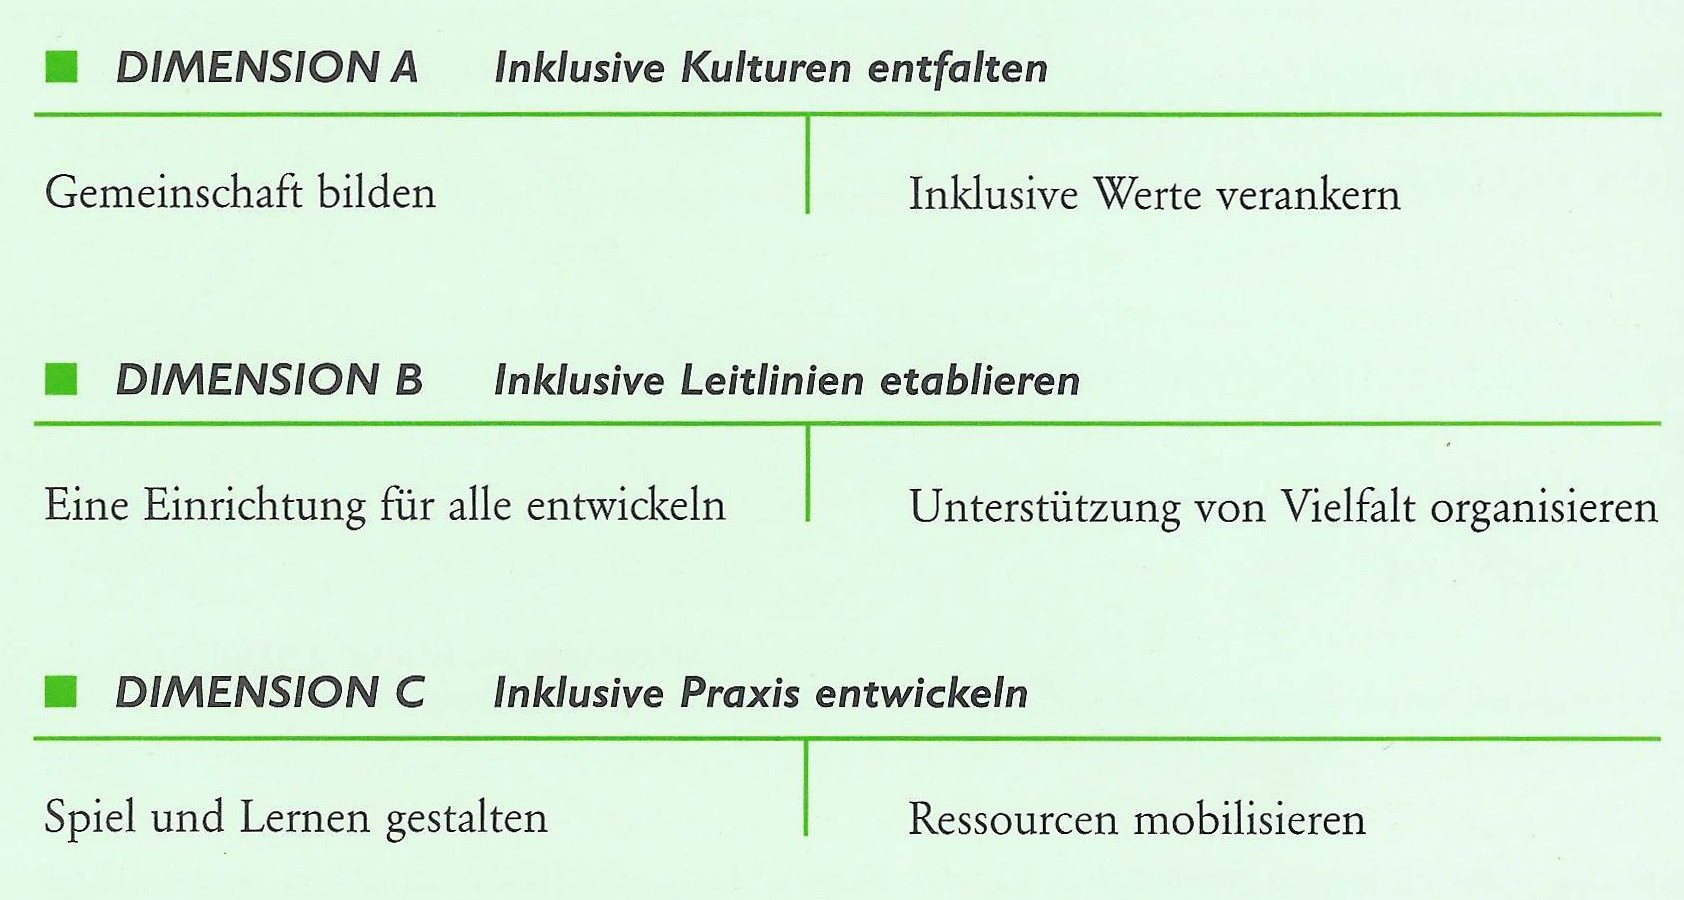
\includegraphics[width=0.8\textwidth]{bilder/planungsrahmen}
  \caption{Planungsrahmen}
\end{figure}

\paragraph{Inhaltsstruktur des Index} Den Planungsrahmen bilden dabei laut der Autoren (2011, 20) drei Dimensionen, die jeweils in zwei Bereiche unterteilt werden (vgl. Tabelle in Abbildung~\ref{pic:planungsrahmen}). 
Diese weisen enge Wechselbezüge auf: Inklusive Kulturen (Dimension A) schafft ein Kindergarten, in dem er sich als sichere, akzeptierende, kooperative und anregende Gemeinschaft entwickelt und dieser inklusive Werte als gemeinsame Basis zugrunde legt. Das setzt voraus, dass allen neuen Kindern, Eltern und Mitarbeitern diese Werte vermittelt und gleichzeitig alle Entscheidungen an selbigen ausgerichtet werden.  
Dementsprechende inklusive Leitlinien (Dimension B) etabliert die Kindergartengemeinschaft, indem sie ihre Bedingungen und Regelungen überprüft und so gestaltet, dass alle Kinder in der Gemeinde aufgenommen und in ihrer Vielfalt unterstützt werden. Inklusive Praktiken (Dimension C) entwickelt der Kindergarten, indem er entsprechende Aktivitäten, Angebote und Lernarrangements bereitstellt und materielle und individuelle Ressourcen mobilisiert, in Bezug auf  die Kinder, die Leitungsgremien der Träger, die Eltern oder das sozialräumliche Umfeld, alles was Spiel, Lernen und Partizipation fördert, kann in Frage kommen.   

\begin{figure}
  \centering
  \label{pic:indexProzess}
  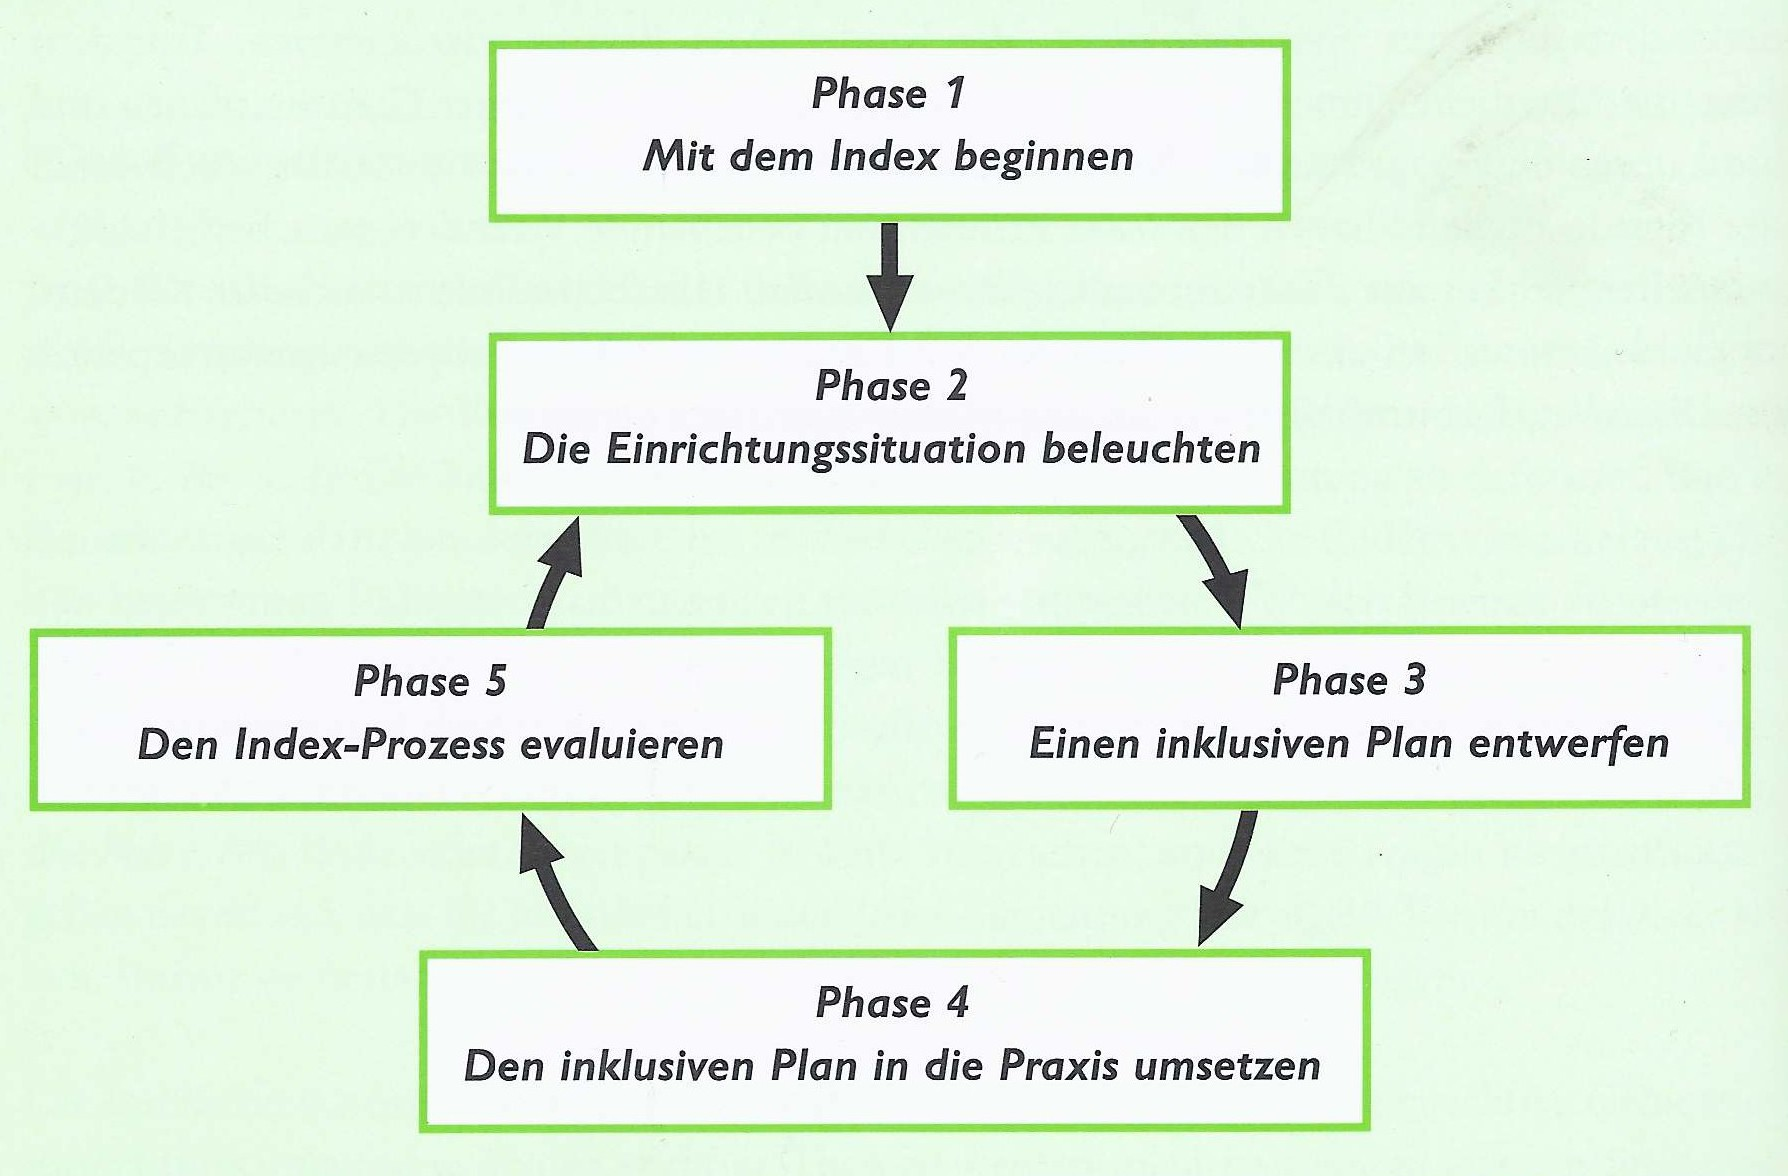
\includegraphics[width=0.8\textwidth]{bilder/indexProzess}
  \caption{Index-Prozess}
\end{figure}

\paragraph{Der Index-Prozess}

Der Index-Prozess selbst zeigt ein Vorgehen in fünf Phasen (vgl. Abbildung~\ref{pic:indexProzess}), was als Orientierung zu betrachten ist, das heißt, dass angepasst an die Situation der Einrichtung gegebenenfalls ein anderes Vorgehen als hilfreicher empfunden wird.  
In Phase 1 des Index-Prozesses „Mit dem Index beginnen“ (Booth et al. 2011, 32) soll das Index-Team gebildet werden, welches sich zunächst mit den Materialien und ihrer Verwendung vertraut macht. Das Index-Team leitet die internen Entwicklungsprozesse der Einrichtung und sollte deshalb strategisch sinnvoll gewählt werden, so dass durch die Personengruppen gute  Voraussetzungen geschaffen werden, die Einrichtung in Richtung Inklusion zu lenken. Auch eine als „kritischer Freund“ bezeichnete Person von außerhalb, jemand, der die Einrichtung kennt, Vertrauen genießt, im Idealfall auch den Index kennt oder noch besser damit arbeitet, kann sich als Moderator einbringen und dem Team helfen, mit kritischen Fragen umzugehen. Seine Funktion ist vielfältig und wird durch den Bedarf ermittelt. Phase 1 dient dazu miteinander und mit den Materialien, den Indikatoren und Fragen, vertraut zu werden, um ein Bewusstsein für den Index zu bekommen. Das setzt auch voraus, dass ein Austausch über das Selbstverständnis von Inklusion stattfindet.  
In Phase 2 „Die Einrichtungssituation beleuchten“ (ebd.) erfolgt eine intensive Bestandsaufnahme. Dabei wird unter Beteiligung der  unterschiedlichen Personengruppen, den Mitarbeitern, der Leitung, der Trägervertretung und den Kindern, zu einem Austausch angeregt, um das Wissen, die Ideen und die Prioritäten möglichst aller Beteiligten herauszufinden. Hierfür sind Indikatoren und Fragebögen für Eltern, Kinder und Mitarbeiter vorgesehen (vgl.~127-137). Je intensiver die Bestandsaufnahme erfolgt und je stärker die Gruppen beteiligt sind, desto qualifizierter und nachhaltiger dürfte die Planung der nächsten Schritte gelingen. 
Phase 3 sieht demnach, „einen inklusiven Plan [zu] entwerfen“ (ebd.), die zuvor erarbeiteten Prioritäten werden mit Hilfe der Handreichung „Prioritäten für die Entwicklung“ (Booth et. al. 2011, 129) zusammengetragen, überarbeitet und letztlich in den Entwicklungsplan und das Konzept eingefügt.
In Phase 4 „Den inklusiven Plan in die Praxis umsetzen“ (Booth et. al. 2011, 32) werden die beschlossenen Prioritäten in die Praxis umgesetzt.  
Booth et. al. (2011, 61) zeigen anhand eines exemplarischen Kindergartens, was Phase 4 zum Inhalt hat: „Wir entschlossen uns, die Leitlinien zum ,sonderpädagogischen Förderbedarf' in Leitlinien zur Inklusion zu ändern. Wir haben jetzt eine ,Inklusionsbeauftragte' statt einer 'Beauftragten für sonderpädagogischen Förderbedarf', aber wichtiger ist, dass sich die Tätigkeit geändert hat, so dass die Bedürfnisse aller Kinder berücksichtigt werden.“   
Es wird empfohlen die Fortschritte zu dokumentieren, so dass diese in Phase 5 „Den Index-Prozess evaluieren“ (ebd.) herangezogen werden können. Im letzten Schritt wird die Arbeit mit dem Index evaluiert, das heißt wiederum, der Prozess wird reflektiert und dokumentiert. Zur Orientierung werden Fragen aufgelistet (2011, 67), zum Beispiel wie gut hat das Index-Team funktioniert oder in welchem Ausmaß gab es ein steigendes Engagement für inklusive Arbeitsweisen? Nach der Evaluation ist im Bemühen um Nachhaltigkeit mit dem Index Prozess fortzusetzen. 
  
Diese fünf Schritte selbst sind so angelegt, dass sie Inklusion befördern und zu dauerhaften Verbesserungen beitragen.

\section{Aktueller Forschungsstand}\label{Forschung}

Um den Stand der Forschung differenziert zu erheben, erschien es sinnvoll sowohl einschlägige Dokumentationen und Diskussionsforen für Forschung heranzuziehen als auch in der Literatur und im Internet gezielt nach Forschungsstudien mit Hilfe der Datenbank der Universität Freiburg zu Inklusion und angrenzenden Themenbereichen wie Integration oder Partizipation im Kontext Kindergarten zu suchen.

Das Ergebnis der Recherche zeigt, dass es bislang nur sehr wenige Veröffentlichungen zu diesen Themenbereichen gibt, vor allem wenige breit angelegte, die auf einer hinreichend großen Datenbasis basieren. Der Grund liegt auf der Hand und ist darin zu suchen, dass Deutschland in Bezug auf die Systemveränderungen hinsichtlich inklusiver Erziehungs- und Bildungsarbeit noch am Anfang steht. Auch wenn es laut Heimlich~\& Behr (2006, 204) Schwerpunkteinrichtungen mit langjährigen Erfahrungen der gemeinsamen Erziehung und Bildung gibt, bilden diese doch die Ausnahme.  
Außerdem nimmt die frühpädagogische Forschung an sich in Deutschland eine vergleichsweise untergeordnete Rolle ein (vgl. Expertenrunde des Staatsinstituts für Frühpädagogik 2003), woraus sich der Mangel an wissenschaftlicher Forschung ebenfalls erklären lässt. 

Tietze et al. (2012, 3) machen darauf aufmerksam, dass trotz vorhandenem Bewusstseins, welche große Bedeutung dem Elementarbereich in Bezug auf die kindliche Entwicklung zukommt, keine validen Daten über die pädagogische Qualität, die Kinder im Kindergarten erfahren, zur Verfügung stehen.
So verfügen kaum ein Träger, Jugendamt oder Ministerium über valide Daten der pädagogischen Qualität von Kindertageseinrichtungen im eigenen Verantwortungsbereich. Das bedeutet, dass elementare Daten für die Qualitätssteuerung fehlen.
Das Informationsdefizit betrifft aber nicht minder auch den wissenschaftlichen Bereich. Es gibt in Deutschland – anders als im anglo-amerikanischen Kontext – bislang keine übergreifend angelegten Untersuchungen zur pädagogischen Qualität in den verschiedenen Betreuungsformen, zu ihren Voraussetzungen wie auch zu Zusammenhängen mit dem Bildungs- und Entwicklungsstand der Kinder. Als Antwort auf diesen Mangel und um zentrale Fragen
hinsichtlich der Qualität in unserem Früherziehungssystem zu
untersuchen, wurde die breit angelegte NUBBEK-Studie durchgeführt, deren Ergebnisse im April 2012 erstmals einer ausgewählten Fachöffentlichkeit und der Presse vorgestellt wurden. 
Der Fokus dieser Studie lag nicht auf Inklusion, die Ergebnisse sind für die Bachelorthesis nur insofern relevant, als dass sie zeigen, wie sich die frühe Bildung, Betreuung und Erziehung für Kinder mit Migrationshintergrund darstellt. 
Laut Tietze et al. (2012, 13 ff.) zeigen die Ergebnisse, dass Kinder mit Migrationshintergrund vergleichsweise spät in öffentliche Einrichtungen  kommen, weshalb ihnen bildungsrelevante Erfahrungen, vor allem im Hinblick auf den Erwerb der deutschen Sprache, verloren gehen. Dem frühzeitigen Besuch der Tageseinrichtung wird eine kompensatorische Wirkung im Hinblick auf den Spracherwerb zugeschrieben. Bei Kindern mit türkischem Migrationshintergrund ist der Eintritt in außerfamiliäre Betreuungssettings durchschnittlich im Alter von 35 Monaten, bei russischem Migrationshintergrund, diese beiden Gruppen stellen den größten Anteil in Deutschland, im Alter von 31 Monaten, während die Kinder ohne Migrationshintergrund im Durchschnitt im Alter von 23 Monaten öffentlich betreut werden. Weiterhin haben die Ergebnisse gezeigt, dass Gruppen mit einem hohen Anteil an Kindern mit Migrationshintergrund eine besonders niedrige Prozessqualität aufweisen. Das heißt, dass gerade diejenigen Gruppen in unserer heranwachsenden Bevölkerung, für die eine qualitativ hochwertige Betreuung und eine optimale Förderung vor Schulbeginn, insbesondere wenn Deutsch die Zweitsprache ist, besonders wichtig sind, eine geringere Chance hierzu haben.
Als Lösung hierzu bietet sich an, gerade diese Einrichtungen besonders zu fördern, durch hoch qualifiziertes Personal und einen verbesserten
Erzieher-Kind-Schlüssel. Außerdem zeigen die Ergebnisse, dass die Qualität der Prozesse innerhalb der zugewanderten Familien ebenfalls vergleichsweise schlechter ausfällt, was sich teilweise aufgrund der schlechteren Ausgangsbedingungen, durch geringeres Einkommen und geringeren Bildungsstand, erklären lässt. 
Zuletzt zeigen die Ergebnisse, dass Kinder mit Migrationshintergrund geringere Kompetenzen in der deutschen Sprache vorzuweisen haben, was nicht überrascht, da die meisten unter ihnen zweisprachig aufwachsen, jedoch in den sprachunabhängigen Kompetenzen zum Teil besser abschneiden als ihre Altersgenossen ohne Migrationshintergrund.
  
Der fehlende Konsens über die Bedeutung des Inklusionsbegriffs hat laut Görannson (2010, 20 f.) Konsequenzen auf die Forschung, da das Verständnis von Inklusion darüber bestimmt, wie über Inklusion geforscht wird. So gibt es verschiedene Fragestellungen, die für die Forschung von Interesse sein könnten. Liegt dem Forschungsinteresse das Verständnis von Inklusion als undifferenzierte Gleichsetzung von Integration zugrunde, impliziert dieses nach Görannson (2010, 21) die Forschungsfrage, ob inklusive beziehungsweise heterogene Gruppen starke soziale Beziehungen unterstützen und ein gutes Lernfeld für jedes Kind ermöglichen. Beinhaltet das Inklusionsverständnis die Notwendigkeit der individuellen Anleitung und Unterstützung des Kindes, um dessen Teilhabe zu erhöhen, so lässt sich laut Serrano~\& Afonso (2010, 44) die Dimension der individuellen Unterstützung an dem Grad messen, in dem sich Kinder aktiv an bedeutungsvollen Lernaktivitäten beteiligen, das heißt anhand des zeitlichen Umfangs, in dem sich ein Kind in einer seiner Entwicklung und dem Zusammenhang gemäßen Art und Weise -- also auf individuellem Kompetenzniveau -- mit seinem Umfeld interagiert.
Inklusion verstanden als langfristiger Prozess der Umstrukturierung verfolgt das Forschungsinteresse einen Beitrag zu leisten zur Herstellung inklusiver Bildungs- und Erziehunseinrichtungen und  andererseits mit Hilfe von empirischer Begleitforschung deren Umsetzung in der Praxis kritisch zu prüfen, was als unbedingt notwendig zu erachten ist, um Inklusion wissenschaftlich zu fundieren und weiter zu entwickeln.

Ein Beitrag zur Herstellung inklusiver Kindertageseinrichtungen ist durch das Projekt QUINTE (Qualitätsstandards für die Integrationsentwicklung in Kindergärten der Landeshauptstadt München) unter der Federführung von Ulrich Heimlich erfolgt. An diesem Forschungsprojekt beteiligten sich laut Heimlich~\& Behr (2006, 200) elf Kindergärten der Stadt München, die in dem Jahr 2002/2003 bereits integrativ arbeiteten. Als Ergebnis dieses Projekts sind 26 Qualitätsstandards als Orientierungsmöglichkeiten für die Integration der frühen Kindheit entwickelt worden, die nun in die Praxis der Kindertageseinrichtungen implementiert und der Entwicklung weiterer inklusiver Einrichtungen zugrunde gelegt werden können. 
Darüber hinaus zeigen die Ergebnisse, dass die integrative Qualität zum gegenwärtigen Zeitpunkt gut entwickelt ist und dass diese Einrichtungen eine größere Zufriedenheit unter den Eltern und Mitarbeitern vorweisen können als Einrichtungen, die nicht integrativ arbeiten. Entsprechend eines inklusiven Verständnisses können als Mängel lediglich die Erreichbarkeit der unterschiedlichen Räume im Sinne der Barrierefreiheit und die Umsetzung der integrativen Therapie genannt werden.  

Inklusive Erziehungs- und Bildungsarbeit kann auch durch die Anwendung des Index für Inklusion unterstützt werden. Haefke~\& Mattke (2011, 134 f.) weisen daraufhin, dass selbige Handreichung im deutschsprachigen Raum jedoch kaum Anwendung findet. Ihre Recherche hat ergeben, dass dieses Hilfsmittel bisher lediglich in Kindertagesstätten in Köln und in zwei Kindertagesstätten in Baden-Württemberg sowie in dem sich auf eine ganze Gemeinde beziehenden österreichischen Inklusionsprojekt in Wiener Neudorf eingesetzt wurde. Die Autoren beschreiben die Erprobung des Index in einer norddeutschen Regelkindertagesstätte und seinen Erfolg auf verschiedenen Ebenen, insbesondere in der beruflichen Kooperation der Erzieherinnen sowie in der Vernetzung innerhalb des Gemeinwesens. Die Vernetzung mit dem Träger konnte mit Hilfe einer Trägervertreterin in das Index-Team deutlich erhöht werden. Die Erfahrung im Team zeigt, dass der Index für Inklusion zunächst als größere Hürde empfunden wurde, sich im Ergebnis jedoch als geeignetes Handwerkszeug erwies. Eine beratende Begleitung von außen wurde als hilfreich empfunden, um mit diesem Hilfsmittel vertraut zu werden. Der Veränderungsprozess war von großer motivierender Wirkung für das Team, da der Index für Inklusion einen Ansatz zur Verbesserung fern von negativ konnotierten Qualitäten wie Überprüfung, Wettbewerb und Versagensangst bereithält.

In Bezug auf den Aspekt 'Unterstützung sozialer Beziehungen' befassen sich einige Veröffentlichungen mit der Frage der Beteiligung von Kindern mit einer Behinderung an der Kindergruppe. Kreuzer (2011, 23-31) gibt einen Überblick über die Ergebnisse der im Zeitraum von 1980 bis 1995 in Deutschland durchgeführten Modellprojekte zur Integration. Auffallend viele Arbeiten sind bedingt durch die üblichen Einzelintegrationsmaßnahmen der Einzelfallforschung zuzuordnen, weshalb sie nicht repräsentativ sind, aber insofern als relevant angesehen werden, als dass sie als Erfahrungswerte in die Weiterentwicklung hin zu Inklusion einfließen können. Gleichzeitig machen sie deutlich, wo Deutschland zu welcher Zeit bezüglich der Integrations-und Inklusionsentwicklung stand. Fritzsche, Schastock~\& Schöler (2005, 80) weisen daraufhin, dass diese Modellprojekte weitestgehend ohne Erfahrungswerte und ohne eine Qualifizierung der Erzieherinnen für den Umgang mit behinderten Kindern auskommen mussten. 

Auch die in den Untersuchungsergebnissen verwendeten Kategorien Behinderung und Nicht-Behinderung bringen das veraltete Integrationsverständnis zum Ausdruck. Kreuzer (2011, 30) kommt zu dem Schluss, dass „solche Generalisierung bezogen auf die Beteiligung im Gruppenalltag nur von geringer Trennschärfe sind“ (Kreuzer 2011, 30) und wenn die festgestellten Unterschiede nur an der Behinderung festgemacht werden, stigmatisierenden Charakter haben. Alternativ dazu und im Sinne von Inklusion würden die wahrnehmbaren Unterschiede an allgemeinen Kriterien wie Alter, Geschlecht, Verhaltensweisen, Basisfertigkeiten entlang interpretiert werden, so dass die Kinder in erster Linie als Mitglieder der jeweiligen Peergruppe verstanden werden. Sowohl Kreuzer als auch Fritzsche et al. (2005, 82) kommen zu dem Ergebnis, dass der Begriff der Behinderung für die Beschreibung eines Zustandes innerhalb des Kindergartensystems ungeeignet ist.  

Folgend werden einige Forschungsergebnisse, die Kreuzer (2011, 26-31) auflistet, zusammengefasst und durch zwei Fritzsche et al. (2005, ?) und Sarimski (2005, ?) ergänzt. 

\begin{itemize}
\item Die Ergebnisse aus der Kasseler Untersuchung von dem Ehepaar Kniel (1984) zeigen, dass behinderte Kinder häufiger als Vergleichskinder alleine oder gemeinsam mit einer oder bei einer Erzieherin spielen sowie dass sie seltener die aktive Rolle im Zusammenspiel einnehmen. Beobachtet werden konnte, dass behinderte Kinder mehr als die Hälfte der Zeit im Parallelspiel verbringen, das heißt, dass sie die gleiche oder eine ähnliche Tätigkeit ausführen, sich aber nicht in wechselseitige Interaktion begeben, etwa 30\,\% der Zeit allein und nur knapp 20\,\% in Kooperation miteinander verbringen. Darüber hinaus konnte gezeigt werden, dass behinderten Kinder ihre Wünsche und Bitten zu 70\,\% an Erwachsene richten, während Vergleichskindern nur zu 40\,\% Erwachsene adressieren. Insbesondere stark motorisch eingeschränkte Kinder fallen durch ihre starke Erwachsenenorientierung ins Auge. Eine ablehnende Reaktionen auf ihre Anfragen erleben sie gleich häufig wie andere Kinder. Ihre Situation in Konflikten entspricht der anderer Kinder, weshalb die Befürchtungen einer 'Sündenbockrolle' unter den behinderten Kindern nicht bestätigt werden konnte. Auffällig war zudem, dass sie anders als die Vergleichskinder den Konstruktions- und Geschicklichkeitsspielen sehr viel weniger Interesse schenken.

\item Im Dortmunder Modellprojekt von Heimlich (1993) konnte beobachtet werden, dass behinderte Kinder eine deutlich verlängerte Eingewöhnungs- und Adaptions\-phase zeigen. Heimlich geht davon aus, dass „die Hauptschwierigkeiten des Integrationsprozesses im ersten Aufenthaltsjahr im Kindergarten zu bewältigen sind“ (Heimlich 2003, 17 in Kreuzer 2011, 27) und die Erzieherinnen für die Gestaltung sozialer Kontakte und die Überwindung möglicher Schwierigkeiten in der Kontaktanbahnung besondere Kenntnisse benötigen.

\item Fichtner und Timmann (1995) schreiben in ihrem Abschlussbericht des niedersächsischen Erprobungsprogramms „Gemeinsame Erziehung“, dass nach Wegen gesucht werden muss, verstärkt Spiel- und Lernprozesse der Kinder untereinander anzuregen. Eine direkte Beteiligung der Fachkräfte würde die Interaktionen jedoch hemmen, da sie sich negativ auf die Selbsttätigkeit auswirkt. Eine Ausnahme bilden schwer- und schwerstbehinderte Kinder, für sie sei die anregende Beteiligung zu Interaktionen von Seiten durch die pädagogische Fachkraft wichtig. 

\item Klein, Kreie, Kron~\& Reiser (1984) beobachteten im Laufe ihrer auf zwei Jahre angelegten Studie, dass wahrnehmungs- und bewegungsbeeinträchtigte Kinder in integrativen Gruppen „Bezugspunkte für Wärme und Zärtlichkeit“ darstellen. Die Zuwendung und Versorgung dieser Kinder geschieht mehr mittels Körperkontakt, weshalb sich der Alltag in integrativen Gruppen im Vergleich zu Regelgruppen insgesamt als körperorientierter beschreiben lässt. 

\item die Ergebnisse der Beobachtungen eines Jungen mit einer schweren spastischen Bewegungseinschränkung von Fritzsche et al. (2005, 106 f.)  zeigen, dass sich die Beschäftigungsangebote der Erzieherin für die ganze Gruppe stark an den Bedürfnissen der nicht-behinderten Kinder orientieren, mit dem Ergebnis, dass für das spastische Kind eine Extrabeschäftigung gefunden werden muss oder es so umfangreiche Hilfe bei der Ausführung der Aufgabe benötigt, dass nicht mehr von Selbsttätigkeit gesprochen werden kann. Die pädagogische Arbeit ist hier noch sehr durch die Orientierung am Ergebnis geprägt, statt dass im Mittelpunkt das gemeinsame Tun und soziale Miteinander steht. In einer Befragung der Erzieherinnen begründen diese ihre Arbeitsweise, indem sie anführen, dass die Eltern solche Ergebnisse sehen wollen würden.

\item Sarimskis (2005) Daten führen vor Augen, dass mit erhöhten Risiken für einzelne Behinderungsformen gerechnet werden muss:
\begin{enumerate}
\item Kinder mit schwerer Hörbehinderung beteiligen sich im Kontakt mit hörenden Kindern gern an Konstruktionsspielen, weniger aber an Rollenspielen. Da sie weniger zum Drehbuch beitragen können, sind sie als Spielpartner offenbar weniger attraktiv.
\item Blinde und hochgradig sehbehinderte Kinder finden insgesamt schwerer einen Einstieg in das gemeinsame Spiel, weil sie das laufende Spielgeschehen nicht verfolgen können, sie haben größere Schwierigkeiten im Freispiel Spielsachen zu finden und sich räumlich zu orientieren.
\item Kinder mit geistiger Behinderung spielen mehr für sich allein, bringen weniger Ideen zum gemeinsamen Spiel ein und sind weniger beliebt als Spielpartner.
\item Kinder mit Autismusspektrumsstörung schauen selten zu ihren Bezugspersonen auf, sind sehr auf den jeweiligen Gegenstand bezogen und scheinen ihre Erfahrungen nicht mit anderen teilen zu wollen. Sie suchen nur Blickkontakt, wenn sie Hilfe benötigen, vor allem bei funktionellen Fragen wie dem Öffnen einer Kiste oder dem Erreichen eines Spielzeugs. 
\end{enumerate}
Eindeutige Ablehnung und Zurückweisung lassen sich für das Kindergartenalter nicht konstatieren, allenfalls geringerer Status und weniger Spielpartner und Freunde.
\end{itemize}
\part{Die empirische Studie: Unter Berücksichtigung welcher Aspekte ist Inklusion im Kindergarten umsetzbar?}
\chapter{Die qualitative Untersuchung}
\section{Forschungsfrage und Begründung des qualitativen Designs}
Das Erkenntnisinteresse der vorliegenden Arbeit besteht darin, Aspekte und Zusammenhänge aufzudecken, die Inklusion im Kindergartenalltag gelingen lassen beziehungsweise erschweren, so dass notwendige, hemmende und fördernde Bedingungen für die Umsetzung von Inklusion gesammelt werden können. Der Gewinn im Identifizieren solcher Mechanismen ist vielfältig. Erstens ist denkbar, dass die befragten Leitungen durch eine Bestandsaufnahme ihre inklusiven Prozesse kritisch hinterfragen und verbessern. Zweitens können weitere Kindergärten aus den empirischen Ergebnissen Schlüsse ziehen, die ihnen Orientierung auf dem Weg zur inklusiven Einrichtung geben. Drittens geben die Ergebnisse darüber Auskunft, was konkret von Seiten der Verantwortungsträger erwartet und gebraucht wird, um das Inklusionskonzept erfolgreich im Kindergarten etablieren zu können.

Die Forschungsfrage, „Unter Berücksichtigung welcher Aspekte ist Inklusion im Kindergarten umsetzbar?“, zielt auf das Aufdecken von sozialen Mechanismen innerhalb der Strukturen des Kindergartens ab. Vielfältige Bezüge fanden im Leitfaden Beachtung, zum Beispiel der Einfluss der Rahmenbedingungen auf Inklusion, des Konzepts, des Inklusionsverständnisses, der pädagogischen Haltung, der mitgebrachten Kompetenzen der Fachkräfte, der Organisationsstruktur der Einrichtung und der Zusammenarbeit im Team. 
Die Forschungsfrage erfordert folglich eine mechanismusorientierte Strategie, die auf der Rekonstruktion von Fällen basiert, keine  standardisierte, die mittels der Aussagen von vielen individuellen Akteuren erhobenen wird, da Qualität und nicht Quantität erhoben werden soll. Als geeignete Vorgehensweise für die Beantwortung der Forschungsfrage wird ein  
qualitatives Forschungsdesign angedacht, da selbiges nicht nur der Rekonstruktion von Fällen oder Prozessen dient, sondern zudem auch immer dort empfohlen wird, „wo es um die Erschließung eines bislang wenig erforschten Wirklichkeitsbereichs“ geht (Flick, von Kardoff und Steinke 2000, 25) -- Inklusion im Untersuchungsfeld Kindergarten stellt einen solchen Wirklichkeitsbereich dar -- und wo es hinsichtlich der Theorieorientierung auf Entdeckung abzielt.
Laut Flick,von Kardoff und Steinke (2000, 45) bedeutet das, dass Theorien und Hypothesen aus den unmittelbar gesammelten Daten entwickelt werden. Diese Annahmen können an der Realität scheitern, weshalb diese an der Realität in einem weiteren Schritt geprüft werden müssen, um bestätigt werden zu können. Der Schritt der Überprüfung kann nicht Inhalt dieser Arbeit sein, da er den Rahmen sprengen würde.  

Um solcherart komplexe Wissensbestände zu rekonstruieren empfehlen Meuser und Nagel (1997, 481) das Experteninterview als eine geeignete Methode. Dieser Empfehlung folgend fiel die Wahl der Methode zur Datengewinnung auf das Experteninterview. 


\section{Die Erhebungsmethode: Experteninterview}
Im Folgenden wird zunächst der Expertenbegriff diskutiert, um darzulegen, wer für das Vorhaben der vorliegenden Arbeit überhaupt als Experte angesprochen werden konnte.
Daran anschließend wird die Auswahl der befragten Experte aufgezeigt. 

\subsection{Der Expertenbegriff}
Gläser und Laudel (2010, 13) verweisen darauf, dass der Begriff ’Experteninterview’ in der sozialwissenschaftlichen Literatur in der Regel an die Expertenrolle des Interviewten im untersuchten sozialen Feld, das heißt, an seine gehobene berufliche Position, gebunden ist (vgl. Meuser und Nagel, 2005, Bogner, Littig und Menz 2005). Entgegen dieser weit verbreiteten Meinung findet sich bei Gläser und Laudel (2010, 11) der bereichernde Gedanke, dass Experten nicht zwingend in einer gehobenen Position zu sein haben, um über ein besonderes Expertenwissen zu verfügen. Jeder Mensch, der einen Erfahrungsbereich für sich erschließt, wird zum Experten. So wird der Musiker, der einen bestimmten Musikstil aufgreift und alles darüber in Erfahrung bringt oder der von einer seltenen Krankheit Betroffene zum Experten für diesen Musikstil oder jene Krankheit. Die Autoren verweisen darauf, dass schließlich jeder Mensch über besonderes Wissen verfügt, nämlich das Wissen über die sozialen Kontexte in denen er agiert, an denen er unmittelbar Anteil hat. Jeder verfügt zum Beispiel über besonderes Wissen über die eigenen Arbeitsprozesse oder über die Organisation, in der er arbeitet. Ein Experte ist im Sinne von Gläser und Laudel (2010, 12) als „Quelle von Spezialwissen über die zu erforschenden sozialen Sachverhalte“ zu verstehen. „Experteninterviews [wiederum] sind eine Methode dieses Wissen zu erschließen.“ Ausgehend von diesem Expertenbegriff kommen für das Untersuchungsfeld Kindergarten sowohl die Leitung der Einrichtung als auch die Erzieherinnen als zu befragende Experten in Betracht. 
 
\subsection{Die befragten Experten}
Die wenigsten Kindergärten weisen sich als inklusiv aus. Das heißt, der Name der Einrichtung ist nicht leitend. Ein Ausschlusskriterium für die Auswahl der Experten war, dass die Einrichtung sowohl von Kindern mit besonderen Bedürfnissen als auch von Kindern ohne besondere Bedürfnisse besucht wird, so dass die Gruppenmischung der gesellschaftlichen Vielfalt entspricht und somit als inklusiv anzusehen ist. Um fündig zu werden, waren sozial schwierige Einzugsgebiete mit einem hohen Anteil an Familien mit einem Migrationshintergrund im Blickfeld, da die Kindergärten zumeist auf die soziale und kulturelle Vielfalt des Einzugsgebietes und somit auf die unterschiedlichen Bedarfslagen der Familien vor Ort Antworten zu finden versuchen und solche Antworten inklusive Prozesse anregen. Da bei diesen Einrichtungen der Anteil der sozial benachteiligten Familien hoch ist, kann nur bedingt von gesellschaftlicher Vielfalt gesprochen werden, da die sozial besser gestellten Familien in ’sozialen Brennpunkten’ gegebenenfalls als Minderheit vertreten sind.    
Weiterhin wurde bei der Auswahl der Einrichtungen berücksichtigt eine gewisse Trägerbreite abzubilden, da die inklusive Ausrichtung der Einrichtung erheblich von der Unterstützung und Steuerung, die sie durch den Träger erfährt, abhängt (vgl. Kapitel~\ref{sec:kitaSelbst} und~\ref{Strukturelle Rahmenbedingungen}), was nicht automatisch heißt, dass dies der Wahrnehmung der Träger entspricht. Es konnten in der Stadt Freiburg im Breisgau\footnote{ Da einige Angebote zur Förderung der Chancengleichheit von der Stadt Freiburg oder von der AWO-Freiburg initiiert wurden, würde das Anonymisieren der Stadt einen großen Informationsverlust bedeuten.} Einrichtungen gefunden werden, deren Träger erstens die Diakonie, zweitens die Arbeiterwohlfahrt (AWO) und drittens die katholische Kirchengemeinde sind. Der Erstkontakt per Telefon erfolgte stets mit der Kindergartenleitung, die sich in allen drei Fällen als Interviewpartner zur Verfügung stellte. 

\section{Datenerhebung}
\subsection{Methode der Datenerhebung: Interviewleitfaden}
Um sich ein Bild vom Arbeitsfeld der Kindergartenleitung zu machen, sah die Gliederung des Gesprächsleitfadens vor, dass die Expertinnen als Einstieg gefragt wurden, wie sich die strukturellen Rahmenbedingungen der Einrichtung beschreiben lassen und welche Kinder die Einrichtung besuchen. Daran schlossen sich Leitfragen zu deren konzeptionellen Überlegungen, deren Inklusionsverständnis, deren Haltung, zum beschrittenen Prozess der Inklusion und seinen Stolpersteinen, zur Kooperation sowohl im Team als auch mit anderen Institutionen und zuletzt zur Partnerschaft mit den Eltern an (vgl. Gesprächsleitfaden im Anhang A).

\subsection{Durchführung der Datenerhebung}
Im Rahmen der Bachelorthesis wurden drei Experteninterviews im Zeitraum vom 15. bis 27.10.2012 durchgeführt. 
Die Anfragen erfolgten durch telefonische Kontaktaufnahme. Im Erstkontakt wurde kurz das Forschungsvorhaben erklärt sowie begründet, warum ein Interesse an der jeweiligen Einrichtung beziehungsweise an der Person vorliegt. Als ’Türöffner’ erwies sich die Information,  wodurch die Aufmerksamkeit auf die Person gelenkt wurde, zum Beispiel durch Presseberichte oder die Empfehlung des Gutachters, der in Kontakt zu der Einrichtung steht. 
Des weiteren wurde angeboten auf Wunsch den Interviewleitfaden zuzusenden, so dass die Fragen von der Leitung vorab eingesehen werden konnten und eine Vorbereitung auf den umfangreichen Leitfaden stattfinden konnte. Davon machten zwei von drei Expertinnen Gebrauch. Das hatte zur Folge, dass die Expertinnen unterschiedliche Voraussetzungen mitbrachten. Einerseits gab es die sehr gut vorbereitete Expertin, die Stichpunkte zu jeder Frage formuliert und die Fragen so verinnerlicht hatte, dass sie bei der Beantwortung der Fragen berücksichtigte, welche Antworten an welcher Stelle ihren Platz finden sollten. Andererseits gab es die Expertin, die unvorbereitet angetroffen, mit der Beantwortung einer Frage viele weitere Bezüge zu anderen Fragen herstellte und in ihren Aussagen eine hohe Spontanität zeigte. Die Durchführung der Interviews zeigte, dass die Auseinandersetzung mit den Fragen vorab Auswirkungen darauf hatte, wie reflektiert, aber auch spontan und damit verbunden emotional beteiligt geantwortet wurde.     
Die Vergleichbarkeit der Interviews wird laut Meuser und Nagel (2005, 81) durch die Nutzung des Leitfadens in der Interviewführung und den „gemeinsam geteilten institutionell-organisatorischen Kontext“ sicher gestellt, weshalb die erwähnten unterschiedlichen Ausgangssituationen, keinen Einfluss auf die Vergleichbarkeit haben.

Der Ort der Befragung war der Arbeitsplatz des Experten, konkret das Büro der Leitung. Die Befragungsdauer variierte zwischen 50 Minuten und zweieinhalb Stunden, wobei ohne Ausnahme alle Fragenkomplexe angesprochen wurden. Die unterschiedliche Interviewdauer ergab sich aus dem Verlauf des jeweiligen Interviews und der zusätzlichen Themen, die von Seiten der Experten angesprochen wurden. In dem zeitlich intensivsten Interview wurde die Aufzeichnung des Interviews verweigert, jedoch darauf hingewiesen, dass Bereitschaft besteht, ausreichende Zeit für das Interview zur Verfügung zu stellen, so dass entsprechende Notizen angefertigt werden konnten, um das Gespräch anschließend in einem Gedächtnisprotokoll zu rekonstruieren. Nach Anfertigung des Gedächtnisprotokolls wurde dieses der Expertin zugesandt, so dass für sie die Möglichkeit bestand, Veränderungen oder weitere Ergänzungen vorzunehmen. Auch den anderen Experten wurden zur Überprüfung die vollständig transkribierten Interviews zugesandt. 
Die Experteninterviews wurden mit Hilfe des Aufnahmegeräts Zoom H2 technisch problemlos auf Tonband aufgenommen und anschließend transkribiert. Parallel zu den Tonaufnahmen wurden Notizen zu den Interviews angefertigt. 

Insgesamt stieß die Befragung bei allen Interviewten auf große Bereitschaft, Neugierde und Interesse für das Thema.

\section{Das Auswertungsverfahren: Qualitative Inhaltsanalyse}

\paragraph{Transkription} Nach Abschluss der Interviewführung erfolgte als Vorbereitung der Qualitativen Inhaltsanalyse die Transkription entsprechend der Vorgaben von Meuser und Nagel (2005, 83). Das bedeutet, die Interviews wurden unter der Wahrung der Anonymität -- inhaltlich vollständig -- verschriftlicht und geglättet und somit von Zwischenlauten, Dialektfärbungen, überflüssigen Redundanzen und Floskeln befreit. Diese Methode fand Anwendung, weil sich die „Auswertung von Experteninterviews an thematischen Einheiten, an inhaltlich zusammengehörigen, über die Texte verstreute Passagen [und] nicht an der Sequenzialität von Äußerungen je Interview“ (Meuser und Nagel 2005, 81) orientiert und somit auf vergleichbare Datengewinnung ausgerichtet ist. 
Ergänzend wurden die Empfehlungen von Mayring (2010, 55) in zwei Punkten berücksichtigt. Er schlägt vor, unverständliche Passagen sowie abgebrochene Sätzen mit Hilfe von drei Punkten (...) und Stockungen, Unterbrechungen oder Gedankensprünge durch einen Gedankenstrich (--) zu kennzeichnen. 
Für das Formatieren wurde außerdem der Hinweis von Gläser und Laudel (2010, 194) berücksichtigt, inhaltlich zusammengehörende Aussagen -- Sinneinheiten -- durch Absätze erkenntlich zu machen. Das heißt, dass eine Antwort des Interviewpartners, vorausgesetzt ein neuer Gedanke kommt hinzu, mehrere Absätze umfassen kann. Eine bessere Lesbarkeit wurde außerdem durch das Kursivsetzen der Interviewfragen erreicht (vgl. Transkripte der Interviews im Anhang C). 

\paragraph{Extraktion} Anschließend wurden die Transkripte mit Hilfe der Qualitativen Inhaltsanalyse entsprechend der Vorgaben von Gläser und Laudel (2010) ausgewertet. Sie (2010, 200 ff.) beschreiben als  Ziel dieses Verfahrens eine neue Informationsbasis zu schaffen, die nur noch die Aussagen enthält, die für die Beantwortung der Forschungsfrage relevant sind. Der Kern dieses Verfahrens ist die Extraktion, die Reduktion des Datenmaterials durch die Fokussierung auf die Forschungsfrage. Extraktion bedeutet konkret, den Textabsatz zu lesen, diesen auf der Grundlage der theoretischen Vorüberlegungen zu interpretieren und zu entscheiden, welche der in ihm enthaltenen Informationen für die Beantwortung der Forschungsfrage relevant sind. Diese Informationen werden in zusammengefasster Form unter  entsprechenden Kategorien und Unterkategorien abgelegt, welche durch die theoretischen Vorüberlegungen entwickelt wurden. Das heißt, die Vorüberlegungen, welche Einflussfaktoren die Umsetzung von Inklusion im Kindergarten begünstigen oder auch behindern -- Gedanken, ohne die der Interviewleitfaden nicht hätte erstellt werden können -- leiten die Extraktion an. Sie ergeben das Suchraster, welches auf den Text gelegt wird. Das Kategoriensystem hat durch die Vorüberlegungen einerseits erste Festlegungen erfahren, wird aber gleichzeitig aus dem Textmaterial heraus neu geformt, was dem Prinzip der Offenheit dieses Verfahrens entspricht. Das Kategoriensystem wird während der Extraktion fortwährend an die Besonderheiten des Materials angepasst. Laut Gläser und Laudel (2010, 262 f.) ermöglicht die Offenheit des Auswertungsverfahrens, dass die empirischen Phänomene nicht unter theoretischen Annahmen subsumiert werden, sondern mit aufgenommen werden, wenn sie theoretischen Vorannahmen widersprechen oder über diese hinausgehen.

\paragraph{Kategoriensystem}
Das ’Kategoriensystem’ als Auswertungsraster beruht laut der Autoren (2010, 206) auf einer Zusammenstellung der theoretisch angestellten Einflussfaktoren und Kausalmechanismen, die Inklusion bedingen und somit die Forschungsfrage repräsentieren. Um das Auswertungsraster zu konstruieren, werden die fünf zentralen Aspekte, die in Kapitel~\ref{sec:Wie} erläutert werden, als so genannte Auswertungskategorien übernommen, die Merkmalsausprägungen dieser zentralen Aspekte bilden im Kategoriensystem die so genannten Dimensionen. 

Die Extraktionstabelle zur Auswertungskategorie 'Strukturelle Rahmenbedingungen' (vgl. Anhang ??) soll als Illustration dienen. 
Die Definition im Theorieteil in Kapitel~\ref{Strukturelle Rahmenbedingungen} mit einem Verweis auf Kapitel~\ref{subsec:Strukturquali} enthält die Dimensionen, die für das Kategoriensystem angenommen werden. „Strukturelle Rahmenbedingungen sind die erwähnten Aspekte, die unter Strukturqualität (vgl. Kapitel~\ref{subsec:Strukturquali}) fallen und somit laut Garai, Kerekes, Schiffer, Tamás, Trócsányi, Weiszburg und Zászkaliczky (2010, 47) im entscheidenden Maße von gesetzlichen, ökonomischen und regierungsamtlichen Entscheidungen abhängen“ (vgl. Kapitel~\ref{Strukturelle Rahmenbedingungen}).
„Laut Tietze (2004, 407) werden unter Strukturqualität Aspekte zusammengefasst, die situationsunabhängig, zeitlich stabil und politisch regulierbar sind. Solche strukturellen Rahmenbedingungen können wiederum unterschieden werden in einerseits der Einrichtung zur Verfügung stehende materielle Ressourcen und andererseits personelle Ressourcen. Unter materiellen Ressourcen werden die vorhandenen Räume und deren Ausstattung, die Finanzierung des Personals, der Betreuungsschlüssel, die Gruppengröße und die Gruppen- und Personalstruktur sowie die vorgesehenen Zeiten für mittelbare pädagogische Arbeit zusammengefasst, unter personelle Ressourcen zählt die Qualifikation der Fachkräfte, festgelegt durch Curriculum und Standards in der Erzieherinnen-Ausbildung (vgl. Kapitel~\ref{subsec:Strukturquali})“ 
„Jerg (2011, 54) sieht die systemerneuernden strukturellen Voraussetzungen vor allem in Veränderungen hinsichtlich des Finanzierungsmodells, der Angebots- und Infrastruktur, verlässlicher Unterstützungsleistung sowie Durchlässigkeit und Demokratisierung der Strukturen. [...] Zudem spielt der Träger bei der Umsetzung von Inklusion eine wesentliche Rolle. In Zusammenarbeit mit der Kommune löst er den politischen Willen zur Inklusion ein und schafft die dafür notwendigen Strukturen (vgl. Kapitel~\ref{Strukturelle Rahmenbedingungen}). 
Ausgehend von diesen theoretischen Vorüberlegungen werden nach Anpassung an die Expertenaussagen folgende Dimensionen in das Kategoriensystem der Auswertungstabelle integriert:  
Räume und Ausstattung, Finanzierung, der Einfluss des Trägers, Gruppenzusammensetzung und Bedarfslagen der Kinder, Personalstruktur, Qualifikation der Fachkräfte, Zeiten für unmittelbare pädagogische Arbeit, Fachkraft-Kind-Relation, notwendige Voraussetzungen von regierungsamtlicher Seite, Blick auf die aktuelle politische Situation, Qualitätsentwicklung.  


\paragraph{Extraktionsregeln und Kausalketten} Information können nicht immer eindeutig einer Auswertungskategorie zugeordnet werden. So konnte es in einigen Fällen nicht vermieden werden, dass in einem Absatz enthaltene Informationen mehrfach unter verschiedenen Kategorien abgelegt wurden. Um das Vorgehen bei Abgrenzungsproblemen transparent zu machen, wurden Extraktionsregeln formuliert. Diese stellen sicher, dass während der gesamten Extraktion einheitlich und somit für den Leser nachvollziehbar und nicht willkürlich vorgegangen wurde. 

Zudem wurden in der Auswertung so genannte Kausalketten berücksichtigt. Diese stellen Verbindungen zwischen den Kategorien her, welche für die Beantwortung der Forschungsfrage von Bedeutung sind, da von einer großen Verwobenheit der Aspekte auszugehen ist. Wenn in einem Absatz Kausalketten berichtet werden, erschwert das die Zuordnung erheblich. Deshalb ist das Kategoriensystem um die Spalten 'Ursache' und 'Wirkung' ergänzt. Dort werden Querverweise zu anderen Kategorien hergestellt oder auch innerhalb derselben Kategorie die Ursachen und Wirkungen vermerkt, die von dem Experten angesprochen wurden.

\paragraph{Aufbereitung der Daten}
Nachdem die Zuordnung aller Sinnabschnitte in das Kategoriensystem erfolgte, wurden die Daten in einem zweiten Schritt aufbereitet, verstreute Informationen wurden entsprechend der Empfehlungen von Gläser und Laudel (2009, 229)  
nach inhaltlichen Gesichtspunkten zusammengefasst und Redundanzen beseitigt, mit dem Ziel das Rohmaterial wiederholt zu reduzieren.
Die Zusammenfassung erfolgte hinsichtlich der Gesichtspunkte: notwendige und hemmende beziehungsweise fördernde Bedingungen für Inklusion. 

\paragraph{Auswertungsstrategien}
In der Auswertung wird laut ihnen (2009, 246 ff.) das Ziel verfolgt, die Forschungsfrage zu beantworten, indem die Kausalmechanismen identifiziert werden, die zwischen Ursachen und Wirkungen vermitteln. Für unsere Forschungsfrage ist zum Beispiel von Relevanz herauszufiltern, welche spezifischen Ausgangsbedingungen -- Ursachen -- dazu geführt haben, dass das Team entschieden hat, dass ein Kind mit besonderem Förderbedarf für die Einrichtung nicht länger tragbar sei -- Wirkung -- und was die Einrichtungen im Umgang mit solchen 'Grenzfällen' voneinander unterscheidet.
Die Autoren empfehlen bei einer geringen Zahl von Fällen, zunächst den Kausalmechanismus jedes Falls zu identifizieren und anschließend diese Mechanismen, die gewirkt haben, vergleichend zu analysieren.

Es gilt Kausalmechanismen auf unterschiedlichen Ebenen aufzugreifen.
Auf der ersten Ebene ist der Fokus auf die individuelle Perspektive der Leitung gerichtet, die ihre Ansicht von den wirkenden Kausalmechanismen erklärt. Dabei handelt es sich um die Interpretation der Beobachterin. Da das Experteninterview die Rekonstruktion von komplexen Wissensbeständen bezweckt, ist die Erklärung der Expertin als  ernstzunehmende Äußerung zu behandeln, trotzdem erhebt sie keinen Anspruch auf Wahrheit und 
Auf der zweiten Ebene wird der Kausalmechnismus des Falles rekonstruiert, der zeigt, 'wie es wirklich war', das heißt, „welche Ursachen in diesem konkreten Fall auf welche Weise welche Wirkung hervorgebracht haben“ (Gläser und Laudel 2009, 248). Hierbei werden auch die Informationen berücksichtigt, die im Widerspruch zueinander stehen.
Die dritte Ebene bezieht sich auf alle Fälle und auf alle Fälle anwendbare Kausalmechanismen, die der Beantwortung der Forschungsfrage dienen. Die unterschiedlichen Verläufe in den Fällen müssen durch das Auftreten oder das Fehlen bestimmter Bedingungen erklärt werden können, die bei allen Fällen zu beobachten sind. 

\section{Auswertungsergebnisse und ihre Interpretation}

Insgesamt gliedert sich die Ergebnisdarstellung in fünf Auswertungspunkte. 
Der Schwerpunkt der Auswertung liegt auf den gemeinsam geteilten Wissensbeständen, wobei dies nicht
bedeutet, dass gegensätzliche Positionen der Experten bei der Ergebnisdarstellung ausgeklammert werden.
 
\subsection{Kategorien in der Auswertung}
\paragraph{Strukturelle Voraussetzungen}

\paragraph{Gruppenzusammensetzung und Bedarfe der Kinder und der Eltern}
Die Gruppenzusammensetzung wird von den Kindergartenleitungen durch Attribute wie 'hohe soziale Vielfalt' oder 'gute Mischung' beschrieben. Die soziale Vielfalt lässt sich erstens dadurch definieren, dass sowohl Kinder aus bildugsorientierten als auch Kinder aus bildungsfernen Elternhäusern gemeinsam die Einrichtung besuchen, letztere sind mit „Themen wie Armut, Ausgrenzung und Beschämung“ (C1,~\ref{C1_1}) konfrontiert; zweitens der Anteil an Kindern mit Migrationshintergrund zwischen 63 und 73 \,\% liegt und drittens, dass aufgrund der Einzugsgebiete, in denen soziale Problemlagen gehäuft vorkommen und der Kindergarten sich für diese unterschiedlichen Problemlagen öffnet, zum gegenwärtigen Zeitpunkt der Datenerhebung Kinder mit sehr unterschiedlichen Voraussetzungen die jeweiligen Einrichtung besuchten: 
In der Einrichtung der Diakonie sind die Angaben allgemein gefasst, wonach festgehalten werden kann, dass Kinder mit diagnostiziertem Förderbedarf aufgrund einer seelischen oder geistigen Behinderung den Kindergarten besuchten. In der Einrichtung der AWO waren fünf Kinder, denen aufgrund einer Behinderung oder einer drohenden Behinderung Integrationshilfe zugesprochen wurde, ein Kind, das an Krebs erkrankt war und sich zum gegenwärtigen Zeitpunkt in Remission befand und große Entwicklungsverzögerungen, insbesondere im sprachlichen Bereich zeigte, ein Kind mit einer Sehbehinderung sowie weitere Kinder mit besonderem Unterstützungsbedarf in verschiedenen Entwicklungsbereichen. 
Im katholischen Kindergarten waren Kinder mit Verhaltensauffälligkeiten und Probleme im sozial-emotionalen, motorischen oder sprachlichen Bereich, konkret drei Kinder mit diagnostizierter Lernbehinderung, zwei Kinder mit Hörbeeinträchtigung, die Hörgeräte trugen sowie Kinder mit Wahrnehmungsproblematiken, bei denen noch eine diagnostische Abklärung bevorstand.
Über die Familien wurde ausgesagt, dass viele aufgrund schlechter beruflicher Perspektive staatliche Unterstützung durch Hartz IV beziehen, dass bildungsferne Eltern im Vergleich zu bildunsorientierten Eltern weniger Interesse an der pädagogischen Arbeit im Kindergarten zeigen und dass ein Zusammenhang gesehen wird zwischen der problematischen Biografie der Eltern und der Entwicklung des Kindes. Die Kindergartenleitung sieht in den fehlenden Lernanreizen und Strukturen zu hause die elterliche Motivation begründet, verlängerte Öffnungszeiten und ein warmes Mittagessen nachzufragen. Die elterliche Haltung wird durch den Satz einer Mutter verdeutlicht: „Ihr könnt meinem Kind mehr beibringen als wir zuhause“ (C3,~\ref{C3_6}).

\paragraph{Räume und Ausstattung}
Fördernde Bedingungen für die Umsetzung von Inklusion werden im Vorhandensein zusätzlicher Räume gesehen, konkret wurden ein zusätzlicher Raum für Sprachförderangebote sowie ein Raum für die heilpädagogische Förderung eingerichtet. Auch wenn die Integrationshilfe, durch Heilpädagogen umgesetzt, das Ziel verfolgt, die Kinder mit besonderen Bedürfnissen in gemeinsame Gruppenprozesse einzubeziehen, wurde die Erfahrung gemacht, dass ein Schonraum als Rückzugmöglichkeit eine Bereicherung für das Kind darstellt, da sich ihm bei Bedarf im Eins-zu-Eins-Kontakt genähert, Nöte besser aufgefangen werden und die Kinder den intensiven Kontakt genießen würden. Ausreichend verfügbarer Raum wird auch als Antwort auf einen hohen Bewegungsdrang gesehen. Als Wunsch wird zudem formuliert, einen zusätzlichen Raum für Elterngespräche zu haben, so dass diese nicht mehr im Büro der Leitung stattfinden müssen und Störungen, wie das Klingeln des Telefons, in der Wahrnehmung der Leitung vermieden werden können. 
Für die Umsetzung von Inklusion wirkt demnach hemmend, wenn die baulichen Voraussetzungen  nur eine begrenzte Anzahl an Räumen zulassen oder wenn der Umbau aus Kostengründen bisher nicht bewilligt wurde. Eine notwendige Voraussetzung für das Gelingen von Inklusion wird im  barrierefreien Bewegen des Rollstuhls gesehen, die Bedingungen 'enge Flure und Türen, die nicht breit genug sind' führen dazu, dass Kinder, die auf einen Rollstuhl angewiesen sind, nicht aufgenommen werden können. Als weitere Hindernisse werden die Erreichbarkeit des Turnraums nur über Treppen, das Fehlen einer Behindertentoilette und Türschwellen genannt, letztere werden  durch das Einfügen eines Holzkeils zu kompensieren versucht, der jedoch beim Schließen der Gruppenraumtür wieder entfernt werden muss. Dieses Beispiel ist signifikant dafür, dass Fachkräfte kaum und nur unter einem erheblichen Mehraufwand in der Lage sind Defizite innerhalb der strukturellen Rahmenbedingungen zu kompensieren.
Inklusion verlangt somit danach, dass bestehender Baubestand entsprechend der Bedarfe verändert wird und schließt darauf: „Wenn man das Ernst nehmen will, muss man richtig viel Geld in die Hand nehmen“ (C1,~\ref{C1_25}). Das Einrichten von Kochmöglichkeiten, um den Wunsch der Eltern nach einem gemeinsamen Mittagessen in der Einrichtung zu beantworten, im Innenbereich Möglichkeiten zu schaffen, dass Kinder mit Wasser spielen können oder vorhandene Materialien, die zur Förderung der Körperwahrnehmung eingesetzt werden können, wie 'Bällebad' oder Therapieschaukel werden als Wünsche benannt, deren Umsetzung in Ermanglung finanzieller Ressourcen noch nicht beantwortet wurden. 
 
\paragraph{Finanzierung}
Der finanzielle Rahmen der Einrichtungen ist begrenzt. Gelder fehlen nicht nur für die notwendigen räumlichen Veränderungen, sondern auch für die Dotierung von Leistungen. So wird zum Beispiel die Leitung für die kontinuierliche Qualitätsentwicklung, die sie im Rahmen des Familiennetzwerks leistet, nicht bezahlt. Außerdem ist dem Bedarf einer stellvertretendem Leitung noch nicht entsprochen worden. 
Durch Spendeneinnahmen werden fehlende finanzielle Mittel kompensiert und Antworten auf Bedarfslagen gefunden, der Ausbau des oberen Stockwerks, neue Projekte wie die Konstruktion Naturpädagogik, die Eltern-Kind-Gruppen und Eltern-Kind-Ausflüge beinhaltet, Bildungsausflüge, wie Theater- oder Museumsbesuche oder Bildungsangebote wie musikalische Früherziehung, der Tanzkurs oder der Schwimmkurs – alles Angebote, die in den Kindergartenalltag eingebunden werden, nicht zuletzt kann durch Spenden die Teilnahme am Mittagessen für Familien, die den Elternbeitrag von einen Euro am Tag nicht leisten können, unterstützt werden.
Je etablierter Spenden aus dem Haus heraus oder durch die Unterstützung des Trägers akquiriert werden, desto mehr Bedarfe können gedeckt werden. „ [...] alle Projekte, die wir haben, bezahlt der Förderverein. Sonst könnten wir diese Arbeit nicht machen“ (C1,\ref{C1_37}).

\paragraph{Einfluss des Trägers}
Die Aufgabe des Trägers als finanzieller 'Unterstützer' wird durch die Kinderarmutskampagne 2012 für den Bildungsbereich durch die AWO-Freiburg: „Wenn ich groß bin, werde ich arm.“ (vgl. Abbildung ??) verdeutlicht, wodurch dem Kindergarten für das Jahr 2012 Spendeneinnahmen in Höhe von 10000 Euro zur Verfügung gestellt wurden, so dass Familien, die sich das Mittagessen für ihre Kinder in der Einrichtung nicht leisten konnten, über einen Gutschein unterstützt wurden. Weitere Spenden wurden für die bereits erwähnten Bildungsangebote und -ausflüge bereitgestellt. Durch den Austausch zwischen Leitungs- und Trägerebene und der konkreten Nachfrage: „Was braucht ihr jetzt vor Ort, welche Bildungsausflüge wären wichtig?“ (C2,~\ref{C2_601}) ist das Bedürfnis nach Unterstützung auf Seiten der Kindergartenleitung erfüllt. Sie gibt zu verstehen, dass sie gern bei der AWO angestellt ist und Wertschätzung durch den Träger erfährt, die sie an das Team weitergibt. 
Die AWO-Freiburg hat einen 'Dankeschön-Abend' für die Spender organisiert, an dem alle Einrichtungen teilgenommen und ihre Bildungsprojekte vorgestellt haben. 

Als fördernde Bedingungen für die Steuerung der pädagogischen Arbeit wird die Möglichkeit benannt autonom Entscheidungen treffen zu können. 
Der zur Verfügung gestellte 'Spielraum' durch die Diakonie bemisst sich daran, dass die Fortbildungen leitungsintern entschieden werden können: „Wir können uns den Themen widmen, die wirklich dran sind. Da steht dieser Träger hinter seinen Einrichtungen, weil die sagen, wir sind hier im Brennpunkt und wenn unsere Leute hier mit diesen Themen kommen, dann sind die dran.“ (C1,~\ref{C1_36}). Der Träger regelt lediglich den Finanzrahmen für die Fortbildungen. Unter diesen Bedingungen kann die Einrichtung am Bedarf orientiert entscheiden, welchen Themen sie sich widmet, was als Voraussetzung für konzeptionelle Weiterentwicklung und hohe fachliche Kompetenz gesehen wird. 
Hierin zeigt sich die Offenheit des Trägers. Diese wird auch beim flexiblem Umgang der katholischen Kirchgemeinde deutlich, die die Gruppengröße von den üblichen 22 beziehungsweise 23 Kindern auf 20 reduziert hat als in einer Gruppe drei Kinder mit diagnostiziertem besonderen Förderbedarf waren. 

\paragraph{Fachkraft-Kind-Relation}
Die Personalbemessung richtet sich nach der Anzahl der Kinder und den Hauptbetreuungszeiten, das heißt, wenn eine Einrichtung verlängerte Öffnungszeiten anbietet, wie in einer Einrichtung bis 18 Uhr, dann ist der Personalschlüssel höher als bei einer Einrichtung, deren Betreuungszeiten 13:30, 14:30 oder 15 Uhr enden. In der Einrichtung mit Öffnungszeiten bis 18 Uhr kommen auf 20 Kinder pro Gruppe 3,2 Stellen.
In den anderen Einrichtungen werden 22 oder 23 Kinder von zwei und 18 oder 19 Kinder von 2,5 Fachkräften betreut.    

\paragraph{Personalstruktur}
Zudem wird das Personal aufgestockt, wenn die Einrichtung von einem hohen Anteil an Kindern mit Migrationshintergrund besucht wird und diese Kinder wiederum einen erhöhten Förderbedarf haben oder die Elternarbeit zum Beispiel durch die Unterstützung der Eltern bei der Antragstellung erschwert ist. Unter Voraussetzung dieser Bedingungen gewährt die Stadt Freiburg seit 2011 eine so genannte Migrationsanteilsaufstockung, die im vorliegenden Fall zur Freistellung der Leitung um weitere 20\,\% führt, so dass für diese Leitung die Freistellung von der mittelbaren Arbeit am Kind 50\,\% beträgt, während die anderen 100\,\% freigestellt sind. 
Neben den Erzieherinnen und Erziehern, eine Stelle innerhalb der drei Einrichtungen ist von einem Mann besetzt, sind zusätzlich Heilpädagogen als Integrationshilfe in der Einrichtung. Integrationshilfe wird je nach Art der Behinderung nach § 35 a oder § 53 SGB VIII beantragt, wird diese bewilligt, kommt die Heilpädagogin an zwei Tagen in der Woche jeweils zwei Stunden in die Einrichtung, um das jeweilige Kind zu unterstützen. Zusätzlich zu der Integrationshilfe kann begleitende Hilfe beantragt werden, in der vorliegenden Einrichtung ist das durch Vorpraktikanten oder junge Menschen, die ein Freiwilliges Soziales Jahr machen, umgesetzt. Die begleitende Hilfe wird von der Heilpädagogin im Umgang mit dem Kind angeleitet. Der Bereich Sprachförderung wird durch qualifiziertes Personal, zum Beispiel eine Heilpädagogin der Sprachheilschule, der Leitung, die an einer halbjährigen Weiterbildung teilgenommen hat, die stundenweise für Sprachförderung angestellt ist, und Logopäden umgesetzt.  
 
 


\chapter*{Literaturverzeichnis}
\addcontentsline{toc}{chapter}{Literaturverzeichnis}

Ahnert, L. (2010): Wieviel Mutter braucht ein Kind? Bindung – Bildung – Betreuung: öffentlich und privat. Heidelberg: Spektrum.

Albers, T. (2011): Mittendrin statt nur dabei. Inklusion in Krippe und Kindergarten. München: Reinhardt.

Becker-Stoll, F. (2009): Wie lernen Kinder in den ersten Lebensjahren? – Entwicklungspsychologische und bindungstheoretische Grundlagen. In: Becker-Stoll, F. und Nagel, B. (Hrsg.): Bildung und Erziehung in Deutschland. Pädagogik für Kinder von 0 bis 10 Jahren. Berlin: Cornelsen, S. 46-54.

Behr, I. (2009): Aspekte inklusiver Qualität in Kindertageseinrichtungen aus Sicht 4- bis 6-jähriger Kinder mit und ohne besondere Bedürfnisse – eine Pilotstudie. Berlin: Dr. Köster.

Belmont, B., Pawlowska, A. und Vérillon, A. (2010):
Partnerschaft mit den Eltern. In: Kron, M., Papke, B. und Windisch, M. (Hrsg.): Zusammen aufwachsen. Schritte zur frühen inklusiven Bildung und Erziehung. Bad Heilbrunn: Klinkhardt, S. 68-75.

Biedinger, N. (2009): Kinderarmut in Deutschland. Der Einfluss von relativer Einkommensarmut auf die kognitive, sprachliche und behavioristische Entwicklung von 3- bis 4-jährigen Kindern. In:  Zeitschrift für Soziologie der Erziehung und Sozialisation, S. 197-214.

%Biewer und Datler (2011): 

Bock-Famulla, K. und Lange, J. (2011): Länderreport frühkindlicher Bildungssysteme 2011. Transparenz schaffen – Governance stärken.
Gütersloh: Bertelsmann.

Booth, T., Ainscow, M. und Kingston D. (2006): Index für Inklusion (Tageseinrichtungen für Kinder). Lernen, Partizipation und Spiel in der inklusiven Kindertageseinrichtungen entwickeln. 4. Auflage, Frankfurt am Main: GEW. 

Bundesministerium für Familie, Senioren, Frauen und Jugend (1992): Übereinkommen über die Rechte des Kindes. Einsehbar unter: http://www.institut-fuer-menschenrechte.de. Stand: 20.12.2012.

Erhardt, K. und Grüber, K. (2011): Teilhabe von Menschen mit geistiger Behinderung am Leben in der Kommune. Freiburg: Lambertus.

Esch, K., Klaudy, E., Micheel, B. und Stöbe-Blossey, S. (2006): Qualitätskonzepte in der Kindertagesbetreuung. Ein Überblick. Wiesbaden: Verlag für Sozialwissenschaften.

Fritzsche, R., Schastock, A. und Schöler, J. (Hrsg.) (2005): Ein Kindergarten für alle. Kinder mit und ohne Behinderung spielen und lernen gemeinsam. 2. Auflage, Weinheim: Beltz. 

Garai, D., Kerekes, V., Schiffer, C., Tamás,
K., Trócsányi, Z., Weiszburg, J. und Zászkaliczky, P. (2010):
Die Rolle der Fachkräfte in der inklusiven Bildung und
Erziehung. In: Kron, M., Papke, B. und Windisch, M. (Hrsg.): Zusammen aufwachsen. Schritte zur frühen inklusiven Bildung und Erziehung. Bad Heilbrunn: Klinkhardt, S. 46-53.

Gastinger, S. und Winkler, J. (2009): Gesetzestexte für Soziale Arbeit. Studienausgabe I: Kinder-, Jugend- und Familienhilfe. Freiburg im Breisgau: Lambertus.

Gastinger, S. und Winkler, J. (2009a): Gesetzestexte für Soziale Arbeit. Studienausgabe II: Soziale Sicherung. Freiburg im Breisgau: Lambertus.

Göransson, K. (2010): Unterschiedliche Perspektiven – unterschiedliches Verständnis von Inklusion. In: Kron, M., Papke, B. und Windisch, M. (Hrsg.): Zusammen aufwachsen. Schritte zur frühen inklusiven Bildung und Erziehung. Bad Heilbrunn: Klinkhardt, S. 17-22. 

Haderlein, R. und Sell, S. (2007): Rahmenbedingungen für gute Bildung -- Herausforderungen für die Pädagogik der Frühen Kindheit. In: Fröhlich-Gildhoff, K., Nentwig-Gesemann, I., Schnadt, P. (Hrsg.): Neue Wege gehen - Entwicklungsfelder der Frühpädagogik. München: Ernst Reinhardt, S. 21-35.

Haefke, S. und Mattke, U. (2011): Ein Kindergarten für Alle. Anwendung und Evaluation des Index für Inklusion in einer Regelkindertagesstätte. In: Teilhabe, Heft 3, S. 134-138.

Hansen, R. Knauer, R. und Sturzenhecker, B. (2011): Partizipation in Kindertageseinrichtungen. So gelingt Demokratiebildung mit Kindern! Weimar: das netz.

Haug, P. (2011): Inklusion als Herausforderung der Politik im internationalen Kontext. In: Kreuzer, M. und Ytterhus, B. (Hrsg.): „Dabeisein ist nicht alles“ -- Inklusion und Zusammenleben im Kindergarten. 2. Auflage, München: Ernst Reinhard, S. 36-52.   

Heimlich, U. und Behr, I. (2005): Integrative Qualität im Dialog entwickeln – auf dem Weg zur inklusiven Kindertageseinrichtun. Münster: Lit. 

Heinze, F. und Prengel, A. (2012): Heterogenität als Grundbegriff inklusiver Pädagogik. In: online-Zeitschrift für Inklusion, Nr. 3. Einsehbar unter: http://www.inklusion-online.net/index.php/inklusion/article/view/161/151, Stand: 16.12.2012.

%Heinze (2011, 10)

Hess, S. (2011): Befähigung zur Zusammenarbeit mit Eltern -- Professionalisierung von Pädagoginnen zur Unterstützung von Familien mit behinderten Kindern und Familien in sozialer Benachteiligung. In: Zeitschrift für Heilpädagogik, Nr. 9, Bad Heilbrunn: Klinkhardt, S. 346-354.  

Honig, M.-S., Joos, M. und Schreiber, N.: (2004): Was ist ein guter Kindergarten? Theoretische und empirische Analysen zum Qualitätsbegriff in der Pädagogik. Weinheim: Juventa.

Hugoth, M. und Jansen, F. (Verband Katholischer Tageseinrichtungen für Kinder (Hrsg.)) (2005): Gute Tageseinrichtungen brauchen gute Träger. Neue Trägerstrukturen und Ansätze zur Weiterentwicklung der Trägerqualität. Bundesverband e.V. Krugzell: Kösel.

Hugoth, M. (2009): Skript der Vorlesung im Sommersemester 2009. 

Hugoth, M. (2010): Organisation von Kindertageseinrichtungen. Studienbrief der Hamburger Fern-Hochschule.

Hugoth, M. und Fritz, A. (2010): Herausforderungen und Perspektiven. Studienbrief der Hamburger Fern-Hochschule.

Hugoth, M. (2011): Inklusion – mal mit der „christlichen Brille“ betrachtet. In: Landesverband katholischer Kindertageseinrichtungen Bayern e.V.: Mitglieder-Info, Heft 1, S. 5-16.

Hüther, G. und Bonney, H. (2011): Neues vom Zappelphilipp. ADS verstehen, vorbeugen und behandeln. 12. Auflage, Ostfildern: Patmos.

Jerg, J. (2011): „Ein Kindergarten für alle“ und „Inklusion von Anfang an“. Entgrenzung als Herausforderung für eine inklusive Gestaltung von Kindertagesstätten. In: Schulz, C. und Stammer, M. (Hrsg.): Von der Kinder- und Jugendhilfe zur Frühkindlichen Bildung. Mulitperspektivische Zugänge zu einer aktuellen Herausforderung. Stuttgart: Evangelische Gesellschaft, S. 46-62. 

Jeske, K. (1997): Mit den Eltern und nicht für die Eltern. Zusammenarbeit von Eltern und Erzieherinnen in Kindertageseinrichtungen. Grafschaft: Vektor.

Karlsson, M. (2010): Die Qualifikation der pädagogischen Fachkräfte -- ein entscheidender Aspekt der Qualität von Kindertageseinrichtungen. In: Kron, M., Papke, B. und Windisch, M. (Hrsg.): Zusammen aufwachsen. Schritte zur frühen inklusiven Bildung und Erziehung. Bad Heilbrunn: Klinkhardt, S. 76-79. 

Klein, F. (2011): Inklusive Erziehuns- und Bildungsarbeit in der Kita. Heilpädagogische Grundlagen und Praxishilfen. Troisdorf: Bildungsverlag EINS.

Klein, F. (2010): Auf dem Weg zur inklusiven Erziehung und Bildung in den Kindertagesstätten der Bundesrepublik Deutschland. In: online-Zeitschrift für Inklusion, Nr.~3. Einsehbar unter: http://www.inklusion-online.net/index.php/inklusion/article/view/73/77 Stand: 14.12.2012.  

%Kobelt Neuhaus, D. (2008): Heterogenität als Motor für Bildungsprozesse -- Kinder mit Behinderung beteiligen und mitnehmen. In: Wagner, P.: Handbuch Kinderwelten. Freiburg: Herder.

Kock,( 2004)

Köhler, H. (2009): Normal ist die Verschiedenheit. Maximen einer gelingenden Integration. In: Erziehungskunst, 11/2009, S. 5-10.

Köpcke-Duttler, A. (2011): Mehr als nur ein Trend. Ethische und rechtliche Begründung der Inklusion. In: Landesverband katholischer Kindertageseinrichtungen Bayern e.V.: Mitglieder-Info, Heft 1, S. 17-23.

Krajewski, M. und Bernhard, T. (2012): Artikel 24 -- Bildung. In: Welke, A. (Hrsg.): UN-Behindertenrechtskonvention. Berlin: Eigenverlag des Deutschen Vereins, S. 164-176.

Krenz (2011, 5)

Kreuzer, M. (2011): Zur Beteiligung von Kindern im Gruppenalltag von Kindergärten – Ein Überblick zu Ergebnissen deutscher Integrationsprojekte. In: Kreuzer, M. und Ytterhus, B. (Hrsg.): „Dabeisein ist nicht alles“ – Inklusion und Zusammenleben im Kindergarten. 2. Auflage, München: Ernst Reinhardt, S. 22-33.

Kron, M. (2002): Gemeinsame Erziehung von Kindern mit und ohne Behinderung im Elementarbereich. In: Eberwein, H. und Knauer, S. (Hrsg.): Integrationspädagogik. Kinder mit und ohne Beeinträchtigung lernen gemeinsam; 6.Auflage, Weinheim: Beltz, S. 178-190. 

Kron, M. (2006): 25 Jahre Integration im Elementarbereich – ein Blick zurück, ein Blick nach vorn. In: online-Zeitschrift für Inklusion, Nr.~1. Einsehbar unter: http://www.inklusion-online.net/index.php/inklusion/article/view/16/16, Stand: 10.05.2012.

Kron, M. (2010): Heterogenität – ein elementarer Aspekt in der inklusiven pädagogischen Arbeit. In: Kron, M. Papke, B. und Windisch, M. (Hrsg.): Zusammen aufwachsen. Schritte zur frühen inklusiven Bildung und Erziehung. Bad Heilbrunn: Klinkhardt, S. 32-41.

Kunkel, P.-C. (2006): Sozialgesetzbuch VIII. Kinder- und Jugendhilfe. Lehr- und Praxiskommentar. 3. Auflage. Baden-Baden: Nomos. 

Kunkel, P.-C. (2010): Jugendhilferecht. Systematische Darstellung für Studium und Praxis. 6. Auflage. Baden-Baden: Nomos. 

Largo, R. H. (2010): Lernen geht anders. Bildung und Erziehung vom Kind her denken. Hamburg: Köber-Stiftung. 

Largo, R. H. (2011): Kinderjahre. Die Individualität des Kindes als erzieherische Herausforderung. 22. Auflage, München: Piper.

Liegle, L. (2006): Soll der Kindergarten die Kinder auf das Lernen in der Schule vorbereiten? In: Friedrich-Ebert-Stiftung (Hrsg.): Droht der Kindergarten zu verschulen? Dokumentation zur Tagung in Stuttgart, S. 5-13.

Meuser, M. und Nagel, U. (2005): ExpertInneninterviews – vielfach erprobt, wenig bedacht. Ein Beitrag zur qualitativen Methodendiskussion. In: Bogner, A., Littig, B. und Menz, W: Das Experteninterview. Theorie, Methode, Anwendung. 2. Auflage, Wiesbaden: Verlag für Sozialwissenschaften.

Ministerium für Kultus, Jugend und Sport Baden-Württemberg (2011): Orientierungsplan für Bildung und Erziehung für die baden-württembergischen Kindergärten. Weinheim: Beltz. Einsehbar unter: http://www.kultusportal-bw.de, Stand: 10.03.2012.

Nagel, B. (2009): Kindorientierte Bildung: Entwicklung des Systems der Tageseinrichtungen für Kinder in Deutschland. In: Becker-Stoll, F. und Nagel, B. (Hrsg.): Bildung und Erziehung in Deutschland. Pädagogik für Kinder von 0 bis 10 Jahren. Berlin: Cornelsen, S. 12-26.

Nagel, B. (2009a): Bildungs- und Erziehungspläne – Perspektiven für die Weiterentwicklung der Kindertagesbetreuung. In: Becker-Stoll, F. und Nagel, B. (Hrsg.): Bildung und Erziehung in Deutschland. Pädagogik für Kinder von 0 bis 10 Jahren. Berlin: Cornelsen, S. 194-207.

Ostner, I. (2008): Ökonomisierung der Lebenswelt durch aktivierende Familienpolitik? In: Evers, A. und Heinze, R. (Hrsg.): Sozialpolitik. Ökonomisierung und Entgrenzung. Wiesbaden: VS-Verlag für Sozialwissenschaften, S. 49-66.

Papke, B. (2010): Bildung und Bildungspläne in der Elementarpädagogik – Chancen für Inklusion, In: online-Zeitschrift für Inklusion, Nr. 3. Einsehbar unter: http://www.inklusion-online.net/index.php/inklusion/article/view/66/71, Stand: 05.11.2012.

Prenzel, M., Carstensen, C., Frey, A., Drechsel, B. und Rönnebeck, S. (2007): PISA 2006 – Eine Einführung in die Studie. In: PISA Konsortium Deutschland (Hrsg.): PISA '06 – die Ergebnisse der dritten internationalen Vergleichsstudie. Münster: Waxmann, S. 31-56.

Roth, H.-J. und Terhart, H. (2010): Migrationshintergrund -- (k)ein frühes Risiko? In: Kißgen, R., Heinen, N. (Hrsg.): Frühe Risiken und Frühe Hilfen. Grundlagen, Diagnostik, Prävention. Stuttgart: Klett-Cotta Verlag, S. 68-83.

Rückert, S. (2011): Herausforderung Kindergarten -- Kindergartenträger und ihre Einrichtungen. Trägeraufgaben und Trägerstrukturen im Wandel. Berlin: Lit.
	
Sander, A. (2004): Konzepte einer inklusiven Pädagogik. In: Verband Sonderpädagogik (Hrsg.): Zeitschrift für Heilpädagogik, Nr. 5, Bad Heilbrunn: Klinkhardt, S. 240-244.

%Sarimski, K. (2011): Soziale Kontakte behinderter Kinder in integartiven Gruppen -- eine explorative Studie im Elementarbereich. In: Zeitschrift für Heilpädagogik, Nr. 1, Bad Heilbrunn: Klinkhardt, S. 4-?.

Sarimski, K. (2012): Behinderte Kinder in inklusiven Kindertagesstätten. Stuttgart: Kohlhammer. 

Sarimski, K. und Schaumburg, M. (2010): Soziale Partizipation in der Freizeit von 3 bis 6-jährigen Kindern mit und ohne Behinderung -- eine vergleichende Elternbefragung. In: Zeitschrift für Heilpädagogik, Nr. 4, Bad Heilbrunn: Klinkhardt, S. 124-129.

%Schädler, J. und Dorrance, C. (2011): Barometer of Inclusive Education – Konzept, methodisches Vorgehen und Zusammenfassung der Forschungsergebnisse ausgewählter europäischer Länder. In: Zeitschrift für Inklusion, Nr. 4.

Schlecht, D., Förster, C., Wellner, B. und Mörth, A. (2008): KITA – Wie gut sind wir? Skalen zur Einschätzung der pädagogischen Qualität nach internationalen Standards unter Einbeziehung aller Bildungspläne in Deutschland. Berlin: Cornelsen. 

Schulz, C. und Stammer, H. (Hrsg.) (2011): Von der Kinder- und Jugendhilfe zur Frühkindlichen Bildung. Mulitperspektivische Zugänge zu einer aktuellen Herausforderung. Stuttgart: Evangelische Gesellschaft.

Schuster, K., Viernickel, S. und Weltzien, D. (2006): Bildungsmanagement: Methoden und Instrumente der Umsetzung pädagogischer Konzepte. Studienbuch 11 zum Bildungs- und Sozialmanagement. Remagen: Ibus.

Serrano, A. M. und Afonso, J. L. (2010): Individualisierte Unterstützungsstrategien in der inklusiven Bildung und Erziehung. In: Kron, M. Papke, B. und Windisch, M. (Hrsg.): Zusammen aufwachsen. Schritte zur frühen inklusiven Bildung und Erziehung. Bad Heilbrunn: Klinkhardt, S. 62-67.

Spaermann (2011): Die Menschwürde kennt keine Kompromisse. Als Gastreferent beim Psychosomatischen Dienstagskolloquium "Seele–Körper–Geist" des Universitätsklinikums Freiburg am 7. November 2011.

Speck-Hamdan, A. (2011): Diversität - Herausforderungen und Chancen für die Pädagogik der frühen Kindheit. Ein Überblick. In: Hammes-Di Bernando, E. und Schreiner, S. (Hrsg.): Diversität. Ressource und Herausforderung für die Pädagogik der frühen Kindheit. Weimar: das netz, S. 14-23.

Tietze, W. (2004): Notwendigkeit und Perspektiven von Qualitätsentwicklung und Qualitätssicherung in Kindertageseinrichtungen. In: Wehrmann, I. (Hrsg.): Kindergärten und ihre Zukunft. Weinheim: Beltz, S. 406-419.

Tietze, W., Dittrich, I., Grenner, K. Groot-Wilken, B., Sommerfeld, V. und Viernickel, S. (2004): Pädagogische Qualität entwickeln. Praktische Anleitung und Methodenbausteine für Bildung, Betreuung und Erziehung in Tageseinrichtungen für Kinder von 0-6 Jahren. Weinheim: Beltz.

Tietze, W., Becker-Stoll, F., Bensel, J., Eckhardt, A. G., Haug-Schnabel, G., Kalicki, B., Keller, H. und Leyendecker, B. (Hrsg.) (in Vorbereitung): NUBBEK -- Nationale Untersuchung zur Bildung, Betreuung und Erziehung in der frühen Kindheit.
Fragestellungen und Ergebnisse im Überblick. Forschungsbericht. Weimar: das netz. Vorläufige Broschüre (2012) online abrufbar unter: http://www.nubbek.de, Stand:  9.11.2012.

Viernickel, S. (2007): Perspektiven der Qualitätssicherung und -entwicklung im System frühkindlicher Bildung, Betreuung und Erziehung. In: Fröhlich-Gildhoff, K., Nentwig-Gesemann, I. und Schnadt, P. (Hrsg.): Neue Wege gehen -- Entwicklungsfelder der Frühpädagogik,  München: Reinhardt, S. 36-47. 

Viernickel, S. und Schwarz, S. (2009): Wie viele Kinder pro Erzieherin? Die Expertise „Schlüssel zu guter Bildung, Erziehung und Betreuung“. Das Leitungsheft Kindergarten heute, Nr. 3, S. 14-16.

Volkert, W. (2008): Die Kindertagesstätte als Bildungseinrichtung. Neue Konzepte zur Professionalisierung in der Pädagogik der frühen Kindheit. Wiesbaden: Verlag für Sozialwissenschaften.

Weiß, H. (2000): Frühförderung mit Kindern und Familien in Armutslagen. München: Reinhardt.

Weiß, H. (2010): Kinder in Armut als Herausforderung für eine inklusive Perspektive. In: Online-Zeitschrift für Inklusion, Nr. 4. Einsehbar unter: http://http://www.inklusion-online.net/index.php/inklusion/article/view/89/92. Stand: 05.11.2012.

Weizsäcker, R. v. (1993): Es ist normal verschieden zu sein. Ansprache bei der Eröffnungsveranstaltung der Tagung der Bundesarbeitsgemeinschaft Hilfe für Behinderte, Gustav-Heinemann-Haus in Bonn. Einsehbar unter: http://www.imew.de/index.php?id=318. Stand: 1.10.2012.

Welke, A. (Hrsg.) (2012): UN-Behindertenrechtskonvention. Berlin: Eigenverlag des Deutschen Vereins. 

%Weber, E. (1999): Pädagogik. Eine Einführung. Band I: Grundfragen und Grundbegriffe. Teil 3: Pädagogische Grundvorgänge und Zielvorstellungen -- Erziehung und Gesellschaft~/ Politik. 8. Auflage. Donauwörth: ?

Wocken, H. (2011): Über die Entkernung der Behindertenrechtskonvention.
Ein deutsches Trauerspiel in 14 Akten, mit einem Vorspiel und einem Abgesang. In: Online-Zeitschrift für Inklusion, Nr. 4. Einsehbar unter: http://http://www.inklusion-online.net/index.php/inklusion/article/view/139/135. Stand: 25.10.2012. 

Wunder, M. (2009): Die UN-Konvention zu den Rechten Behinderter – ein Prüfstein für den zukünftigen Umgang mit Menschen mit Behinderung oder psychischer Erkrankung. In: Online-Zeitschrift für Inklusion, Nr. 2. Einsehbar unter: http://http://www.inklusion-online.net/index.php/inklusion/article/view/37/44. Stand: 14.12.2012.  


\newpage
%\pagenumbering{roman}

% Anhang
\appendix
\chapter{Gesprächsleitfaden der Experteninterviews}\label{Interviewleitfaden}
\paragraph{Strukturelle Rahmenbedingungen und das Inklusionskonzept}
\begin{enumerate}
\item Können Sie etwas zur Organisation und zur Struktur Ihrer Einrichtung sagen?
\begin{itemize}
\item Welche Kinder besuchen Ihre Einrichtung? Welcher sozialen Herkunft sind diese Kinder? 
\item Werden Kinder mit besonderen Bedürfnissen betreut?
\item Personalschlüssel? Gruppengröße?
\item Wie ist das Team zusammengesetzt?
\item Spielen Heilpädagogen oder andere Fachleute mit Spezialwissen eine aktive Rolle im Gruppenalltag?
\item Gibt es Ansprechpartner, die bei Fragen einbezogen werden, wie die Entwicklung eines Kindes möglichst optimal zu unterstützen ist? 
\item Mit welchen Kooperationspartnern ist die Einrichtung vernetzt?
\end{itemize}
\item Gibt es für die Kinder mit besonderen Bedürfnissen konzeptionelle Überlegungen? Entsprechen diese Ihrem Inklusionsverständnis?
Was verstehen Sie unter Inklusion in Bezug auf den Kindergarten? 
\item Können Sie noch weitere Angaben über den Charakter des Konzepts hinsichtlich Inklusion machen?
\begin{itemize}
\item Wie wird der Verschiedenheit der Kinder Rechnung getragen?
\item Wie ist individuelle Unterstützung in Ihrem Konzept vorgesehen?
\item Wie wird die individuelle Arbeit am Kind in das Gruppengeschehen integriert?
\item Was sind gegebenenfalls Strategien, um Therapien in einer inklusiven Form anzubieten?
\end{itemize}
\item Was sind Ihrem Ermessen nach notwendige Voraussetzungen für das Gelingen von Inklusion, die von „oben“ garantiert werden sollten? 
\item Gibt es bildungspolitische Entscheidungen, die der Umsetzung von Inklusion im Weg stehen? 
Wenn ja, was sollte sich ändern? 
Was kann der Träger dazu beitragen? 
Wo sehen Sie Ihre besonderen Aufgaben als Leitung?
\end{enumerate}

\paragraph{Schritte in Richtung Inklusion}
\begin{enumerate}
\item Welche Schritte wurden konkret unternommen, um Inklusion einzuleiten?
\item Was waren und sind Stolpersteine auf dem Weg zur inklusiven Bildungseinrichtung? 
\end{enumerate}

\paragraph{Herausforderungen an das Team}
\begin{enumerate}
\item Welche Herausforderungen werden an das Team gestellt, wenn das Konzept in Richtung Inklusion umgestellt wird?
\item Was sind häufige Fragen der Erzieherinnen, die anzeigen, dass Beratungs- oder Unterstützungsbedarf besteht?
\item Gab es oder gibt es Ängste unter den Mitarbeitern? Welcher Art? Wie wird damit umgegangen?
\item Welche Unterstützung erfährt das Team? 
Gibt es eine gemeinsame Planung und Zusammenarbeit unter den Beteiligten? Gibt es Teamsitzungen, in denen das Verhalten von Kindern diskutiert wird? 
\item Brauchen Erzieherinnen Zusatzqualifikationen, um inklusiv zu arbeiten? 
In welchen Bereichen sind Kenntnisse Ihrer Meinung nach hilfreich?
\item Welches Handwerkszeug müssen ErzieherInnen mitbringen bzw. was macht gute Erzieherinnen aus?
\end{enumerate}

\paragraph{Partnerschaft mit den Eltern}
\begin{enumerate}
\item Welche Bedeutung hat die Elternarbeit im Hinblick auf Inklusion?
Wie werden die Eltern bei Entscheidungen eingebunden? 
\item Was wird in Ihrer Institution organisiert, um eine Beziehung zu den Eltern aller Kinder aufzubauen?
\item Kennen Sie die Einstellungen der Familien zu Fragen inklusiver Erziehung und wie unterstützen Sie den Dialog darüber?
\end{enumerate}

\paragraph{Persönliche Haltung zu Veränderungen und Grenzen der Inklusion}
\begin{enumerate}
\item Haben Sie durch die Umsetzung von Inklusion Veränderungen bei sich feststellen können? Bei den pädagogischen Mitarbeitern? Bei den Kindern? 
\item Wie ist ihr Standpunkt zu der Aussage: „Allen Kindern gerecht werden“? Sehen Sie Grenzen der Inklusion?
\end{enumerate}


\chapter{Kategoriensystem}
\label{Kategoriensys}

% Beginn Querformat
\begin{landscape}
\begin{small}

% ============================
%         Tabelle 5
% ============================
\begin{centering}
%\addcontentsline{toc}{table}{Tabelle 5}
\begin{longtable}{p{2.2cm}p{5.5cm}p{5.5cm}p{5.5cm}p{2cm}} 
\caption{Extraktionstabelle zur Auswertungskategorie \glq Strukturelle Rahmenbedingungen\grq}\\
\toprule
\textbf{Dimension} & \textbf{Sachverhalt (Aussagen konzentriert)} & \textbf{Ursache} & \textbf{Wirkung} & \textbf{Quelle}\\
\midrule
\endfirsthead
\toprule
Dimension & Sachverhalt (Aussagen konzentriert) & Ursache & Wirkung & Quelle\\
\midrule
\endhead
\bottomrule
\endfoot
\multicolumn{5}{l}{\emph{Räume / Ausstattung}}\\
\multicolumn{5}{l}{\emph{– fördernde Bedingungen:\vspace{0.5em}}}\\ %\cmidrule{2-5}
& Extraraum nur Sprache & & & C1 \ref{C1_18}\\ \cmidrule{2-5}
& heilpädagogische Zimmer als Rückzugmöglichkeit & bei hoher Bedürftigkeit des Kindes, braucht jemanden für sich alleine, der sich ihm nähert, so dass Belastungen aufgefangen werden können & Kinder genießen Eins-zu-Eins-Kontakt & \ref{C1_22}\\ \cmidrule{2-5}
& während Freispielzeit zusätzlicher Gang als Antwort auf einen hohen Bewegungsdrang\vspace{1em} & & &  C3~\ref{C3_3}\\
\multicolumn{5}{l}{\emph{– hemmende Bedingungen: \vspace{0.5em}}}\\ %\cmidrule{2-5}
& Speicherausbau langwierig & & & C1\ref{C1_47}\\ \cmidrule{2-5}
& räumliche Stolperfallen: Tür\-schwellen in den Gruppenräumen, ungeeignete Türen,  & alter Baubestand, Umbau bisher nicht bewilligt, Kostenfrage & Türschwellen problematisch für Kind, das krabbelte oder Rollstühle $\rightarrow$ zu kompensieren versucht durch Holzkeil, Holzkeil musste zum Schließen der Tür wieder entfernt werden & C2~\ref{C2_78} \\ \cmidrule{2-5}
& aufgrund baulicher Voraussetzungen wenig Zusatzräume, enge Flure hinderlich für das Durchkommen mit dem Rollstuhl & & Grenzen der Inklusion für Kinder im Rollstuhl & C2\ref{C2_80} \\ \cmidrule{2-5}
& Türen müssen breit genug sein & & & C3~\ref{C3_52}\\ \cmidrule{2-5}
& fehlende Möglichkeiten zum Kochen & & Bedarf der Eltern noch nicht beantwortet & C3~\ref{C3_7}\\ \cmidrule{2-5}
& Umgestaltung von Räumlichkeiten & & & C3~\ref{C3_506}\\ \cmidrule{2-5}
& Turnraum nur über Treppe zu erreichen\vspace{1em} & & & C3~\ref{C3_58}\\ 
\multicolumn{5}{l}{\emph{– notwendige Voraussetzungen:\vspace{0.5em}}}\\ %\cmidrule{2-5}
& Freizügigkeit für Kinder im Rollstuhl für barrierefreies Schieben & & & C3~\ref{C3_508}\\ \cmidrule{2-5}
& Behindertentoilette, breite Türen & & & C3~\ref{C3_52}\\ \cmidrule{2-5}
& ausreichend Räumlichkeiten und finanzielle Ressourcen für Ausstattung: zur Förderung der Körperwahrnehmung: Bälle-Bad, Therapieschaukel, Erfahrungen mit Wasser (keine Möglichkeiten im Innenbereich vorhanden) und ruhige Atmosphäre für Elterngespräche gewünscht (im Büro Unterbrechungen durch Telefonanrufe) & & & C3~\ref{C3_49}\\
\end{longtable}
\end{centering}

% ============================
%         Tabelle 1       
% ============================
\begin{centering}
%\addcontentsline{toc}{table}{Tabelle1}
\begin{longtable}{p{2.2cm}p{8cm}p{6cm}p{3cm}p{2cm}} 
\caption{Extraktionstabelle zur Auswertungskategorie „Rolle der pädagogischen Fachkraft“}\\
% =========================== ANFANG =============================
% ========== Tabellenkopf für erste Seite der Tabelle ============
% ================================================================
\toprule
Dimension & Sachverhalt (Aussagen konzentriert) & Ursache & Wirkung & Quelle\\
\midrule
\endfirsthead
% ============================ ENDE ==============================

% =========================== ANFANG =============================
% ======= Tabellenkopf für jede weitere Seite der Tabelle ========
% ================================================================
\bottomrule
Dimension & Sachverhalt (Aussagen konzentriert) & Ursache & Wirkung & Quelle\\
\midrule
\endhead
% ============================= ENDE ==============================

% ====================== ANFANG Tabellenfuß =======================
\bottomrule
\endfoot
% ============================= ENDE ==============================

% ======================== Tabelleninhalt =========================

\end{longtable}
\end{centering} 

% ============================
%         Tabelle 4       
% ============================
\begin{centering}
\begin{longtable}{p{2cm}p{11cm}p{3cm}p{3cm}p{2cm}} 
\caption{Extraktionstabelle zur Auswertungskategorie „Antworten auf die unterschiedlichen Bedarfslagen“}\\
\toprule
Dimension & Sachverhalt (Aussagen konzentriert) & Ursache & Wirkung & Quelle\\
\midrule
\endfirsthead
\toprule
Dimension & Sachverhalt (Aussagen konzentriert) & Ursache & Wirkung & Quelle\\
\midrule
\endhead
\bottomrule
\endfoot
\end{longtable}
\end{centering} 

% ============================
%         Tabelle 3       
% ============================
\begin{centering}
\begin{longtable}{p{2cm}p{11cm}p{3cm}p{3cm}p{2cm}} 
\caption{Extraktionstabelle zur Auswertungskategorie „Partnerschaft mit den Eltern“}\\
\toprule
Dimension & Sachverhalt (Aussagen konzentriert) & Ursache & Wirkung & Quelle\\
\midrule
\endfirsthead
\toprule
Dimension & Sachverhalt (Aussagen konzentriert) & Ursache & Wirkung & Quelle\\
\midrule
\endhead
\bottomrule
\endfoot


\end{longtable}
\end{centering} 

% ============================
%         Tabelle 2       
% ============================
\begin{centering}
\begin{longtable}{p{2cm}p{11cm}p{3cm}p{3cm}p{2cm}} 
\caption{Extraktionstabelle zur Auswertungskategorie „Kooperation“}\\
\toprule
Dimension & Sachverhalt (Aussagen konzentriert) & Ursache & Wirkung & Quelle\\
\midrule
\endfirsthead
\toprule
Dimension & Sachverhalt (Aussagen konzentriert) & Ursache & Wirkung & Quelle\\
\midrule
\endhead
\bottomrule
\endfoot

\end{longtable}
\end{centering} 

% Ende Querformat und kleine Schrift
\end{small}
\end{landscape}


\chapter{Transkripte der Experteninterviews}\label{Transkripte}
\section{Kindergarten 1: Diakonie}
\begin{linenumbers*}
\emph{F: Können Sie etwas zur Organisation und zur Struktur Ihrer Einrichtung sagen, welche Kinder kommen her, aus welcher sozialen Lage?}\\
A: Bei uns ist eine sehr hohe soziale Vielfalt vertreten, also Kinder aus sehr belasteten, bildungsfernen Familien bis hin zu Kindern, die aus sehr gut organisierten Familien kommen. \linelabel{C1_1001}

Viele Familien haben mit dem Thema Armut zu tun, Ausgrenzung, Beschämung -- und andere, die sind ganz gut integriert. \linelabel{C1_1}

Diese Mischung ist für unsere Arbeit sehr wichtig, dass wir keine Monokultur haben.\linelabel{C1_2}

\emph{F: Können Sie auch etwas zum Anteil der Kinder mit Migrationshintergrund sagen?}\\
A: Also es sind gut Zweidrittel oder sogar ein bisschen mehr im Moment. \linelabel{C1_3}

\emph{F: Betreuen Sie auch Kinder mit besonderen Bedürfnissen, also Kinder mit Behinderung?}\\
A: Ja, wir haben auch Kinder bei uns, die seelische Behinderungen haben, geistige Behinderungen -- körperlich Einschränkungen schon auch mal, aber jetzt nicht so gravierend -- schwerbehinderte, körperlich behinderte Kinder, die haben wir jetzt weniger.\\
\emph{F: Bedingt durch das Milieu sehen Sie wahrscheinlich den Zusammenhang, dass seelische Behinderungen auftreten, Sie haben jetzt kein Kind mit Diagnosen wie Down-Syndrom?}\\ 
A: Ja, wir haben es bei uns gehäuft -- also seelische Behinderungen sind sehr oft und geistige Behinderungen kommen auch nicht selten vor oder Kinder, die Autismus haben -- also das ist schon auch bei uns, ja.\linelabel{C1_4}

\emph{F: Können Sie noch etwas zum Personalschlüssel sagen und zu der Gruppengröße. Ich sehe gerade, sie haben vier Gruppen.}\\
A: Ja, wir haben vier Gruppen jetzt hier. Das sind ungefähr 18, 19 Kinder pro Gruppe. Ich habe pro Gruppe 2,5 Fachkräfte und wir haben durch die Angebote, die wir im Familiennetzwerk haben, aber zusätzliche Menschen, die hier die Arbeit mit uns gestalten, \linelabel{C1_5}

im Bereich Naturpädagogik, Heilpädagogik, im Sprachbereich, also Logopäden, auch noch eine Spracherzieherin ist bei uns. Dann haben wir im Ehrenamt \emph{Bücherwurmfrauen}, dann haben wir Sportler, die bei uns hier die \emph{Ringergruppe} machen.\\ 
\emph{F: Die kommen in die Einrichtung und sind im Gruppenalltag präsent und integriert?}\\ 
A: Nein, nein, nein, nein -- das sind bestimmte Projekte.
Das heißt, es sind Menschen, die eine gewisse Qualifikation haben, die wir hier für die Kinder brauchen \linelabel{C1_6}

und die dann in Kleingruppen diese Angebote durchführen. Die Kinder werden denen sozusagen im Alltag zugeführt -- die haben dann ihre Ringergruppe zum Beispiel. Da kommt dann der Adolf Seger, der war zwölf Mal Weltmeister, und die Papis laden wir dazu ein und dann wird gekämpft und im Vorfeld backen die schon mit unseren männlichen Erziehern Kuchen. \emph{Männer backen für Männer} heißt das Programm und nach dem Sport gibt es Männercafé. Das sind quasi Projekte, die wir mit anderen Menschen durchführen, die da Kompetenzen haben und sie aber in den Alltag der Kinder integrieren -- das sind aber jetzt keine Menschen, die hier Gruppenarbeit im klassischen Sinne übernehmen. Das ist das festangestellte Personal.\\
\emph{F: Ich wiederhole nochmal, ob ich es richtig verstanden habe. Sie nehmen Kinder raus oder sagen die sind geeignet für die Gruppe und die treffen sich dann.}\\
A: Die, die wollen -- wo die Eltern sich zum Beispiel anmelden. Die Ringergruppe ist für das ganze Haus und das wird dann bekannt gegeben und die melden sich dann und wir nehmen aber auch Jungs rein, die keine Papas haben, die mit können oder manchmal verschwinden die Väter ja auch und die kriegen dann die Kerle. Da geht es um ein geschlechtsspezifisches Projekt und da geht es wirklich darum, dass die auch männliche Identifikationsmöglichkeiten haben, weil das einfach verloren geht. Da gucken wir und so haben wir verschiedene Gruppen bei uns -- also die so funktionieren, die aber quasi in den Alltag der Kinder sich wirklich mühelos einbinden.\linelabel{C1_7}

\emph{F: Gibt es auch Ansprechpartner, die sie hinzuziehen oder befragen, wenn Sie Fragen haben, wie die Entwicklung zu unterstützen ist, also wenn sie spezifische Fragen zur Entwicklung von einem Kind haben. Rufen Sie dann jemanden an oder kooperieren sie dann mit jemandem?}\\
A: Ja, ich meine, wir sind natürlich alle sehr fachkompetent, deswegen sind wir auch Pädagogen. Wir sind ja hier keine Bäckerverkäuferinnen. Wir haben schon eine hohe Fachkompetenz und die Entwicklung der Kinder... \linelabel{C1_8}

Bei uns ist es so, dass es ein Dialog gibt im Team, jede Woche, wirklich wie mit der Lupe. 
Und wir haben auch Heilpädagogen und Sprachtherapeuten hier im Haus, also das heißt, die sind vor Ort und da gibt es natürlich durch das Interdisziplinäre einen regen Austausch. \linelabel{C1_9}

Und wenn dann besondere Situationen darüber hinaus für uns relevant sind -- das passiert meist in Gefährdungssituationen, dann laden wir die entsprechenden Beratungsstellen oder die Gruppen wie \emph{Wildwasser}, \emph{Wendepunkt}, wenn es um Missbrauch geht -- zur Fallsupervision ein. Das läuft dann über den Weg nochmal. \linelabel{C1_10}

Wir haben auch eine Musikpädagogin im Haus. Erstmal werden unsere verschiedenen...\linelabel{C1_11}

\emph{F: Was heißt im Haus? Sind die jeden Tag da?}
A: Eben so wie sie in den Projekten arbeiten -- aber dadurch, dass sie vor Ort sind, besteht der unmittelbare Austausch mit dem Fachpersonal.
Das heißt, es sind alles Kleingruppen und es ist auch immer jemand von den Erziehern dabei -- es wird nie etwas ohne eine pädagogische Fachkraft von uns stattfinden -- dadurch besteht schon der Austausch und das wird dann jede Woche im Team gebündelt -- durch den Austausch, die Wahrnehmung. Von daher haben sich die Chancen für die Kinder, die hier sind, unglaublich erhöht, weil der Blick auf ihre Entwicklung ist hier schon sehr pointiert -- das muss man schon sagen. \linelabel{C1_12}

Und was drüber hinausgeht, wie gesagt, manchmal gibt es auch Suchtthemen -- da gibt es dann den kommunalen Suchtbeauftragten, also die Leute holen wir uns dann ran. \linelabel{C1_13}

\emph{F: Mit welchen Kooperationspartnern ist die Einrichtung vernetzt?}
A: \emph{pro familia}, Schulen, Logopädische Praxis, mit der Heilpädagogik, dann die Ärzte hier im Quartier, die Polizei im Stadtteil, Hochschulen auch. Wir haben da ein recht breites Bündnis, kann man im Grunde genommen sagen.
\emph{Südwind},
mit denen machen wir die ganzen Deutschangebote hier für Eltern -- oben ist jetzt gerade ein Deutschkurs -- an vier Vormittagen für Frauen und eine Babygruppe haben wir -- da ist schon alles sehr gut vernetzt. \linelabel{C1_14}

\emph{F: Gibt es so etwas wie konzeptionelle Überlegungen für die Kinder mit besonderen Bedürfnissen?}\\
A: Die Antwort habe ich Ihnen quasi jetzt schon durch das, was ich erzählt habe, gegeben.\\

\emph{F: Oder können Sie sagen, was Sie verstehen unter Inklusion im Bezug auf Kindergarten?}
A: Ich denke, die Idee der Inklusion ist, dass sich die Einrichtung so auch
verändert, um dem Kind quasi Bildungsangebote in der Einrichtung zu ermöglichen
-- also das würde ich mal klipp und klar sagen. Darin liegt natürlich die
Herausforderung, weil jeder Mensch kommt so, wie er ist und hier in
{[Stadtteil]} haben wir sehr viele, sage ich mal, einmalige Menschen. Dieses Konzept, was Sie hier schon antreffen, ist schon ein Ergebnis davon -- also das, was wir hier unter Familiennetzwerk verstehen, ist schon die Bündnisarbeit, um diese Unterschiedlichkeit, oder die Themen, die hier auftreten, noch einmal individuell zu beantworten. 
Wir haben einen großen Fachbereich nur Elternbildung. Wir haben auch in der Naturpädagogik Eltern-Kind-Gruppen. Wir machen am Wochenende Familienausflüge mit Kindern. Es besteht eine ganz enge Interaktion in die Familie -- und das sind alles schon Entwicklungen von einer Kindertagesstätte im Rahmen -- um das schon zu beantworten, um zu sehen, hier gibt es ganz viele Themen, auch Bildungsthemen für Kinder und die Eltern.
Sie müssen ja die Eltern mit rein nehmen. Sie können ja nicht sagen, ihr Kind bilden wir und sie lassen wir gerade mal links liegen. Das geht nicht. Wer mit den Kindern arbeitet, muss mit den Familien arbeiten -- und da denke ich, hat dieses Haus, und das haben Sie ja auch schon in der Homepage gesehen, ganz interessante Antworten entwickelt. Und das sind schon... Das geht in die Richtung. \linelabel{C1_16} 

Die Entwicklung dieser Antworten findet bei und in der Zukunftswerkstatt statt. Es gibt eine Zukunftswerkstatt, und da werden die Themen in der Kita gemeinsam erörtert, mit dem Fachpersonal, mit den Eltern, mit dem Träger oder auch Stellen von außen und so wird quasi die pädagogische Qualität in der Einrichtung weiter verbessert.
\emph{F: Wie oft findet so etwas statt?}\\
A: Je nach Situation. Das kann mal sehr eng maschig sein, dann kann mal wieder ein bisschen Ruhe sein -- das schadet auch nichts.\\ 
\emph{F: Haben Sie einen festen Stamm, der da immer kommt?}\\
A: Wichtig ist, dass die Plätze besetzt sind: die Elternperspektive, die Mitarbeiterperspektive, Gesetz dem Fall auch die Trägerperspektive oder was wir immer auch machen, die Gesetzes gebende Perspektive, die Wissenschaften. Das ist eine ganz, ganz sehr fein gefächerte Art zu arbeiten, wo alle Positionen zu einem Thema erst einmal aufgegriffen werden und dann -- der zweite Schritt ist -- dann wird erörtert, wo ist der nächste Handlungsschritt -- und so hat sich in den letzten Jahren dieses Haus entwickelt. 

\emph{F: Ah, mit Hilfe dieser Werkstatt.}\\ 
A: Der Hintergrund ist eine dialogische Qualitätsentwicklung und ich habe diese Qualifikation -- das heißt, dass es ein Dialogverfahren gibt, wo man gemeinsam das verändert -- also nicht hinwegsetzt und sagt: „O.k., das ist jetzt gerade in, wir machen das!“ -- so läuft das hier niemals.\\
\emph{F: Demokratische Strukturen.}\\
A: Ja, basisdemokratisch, Eltern werden beteiligt und vor allem immer geguckt, was ist hier eigentlich los. Also es nützt ja nichts, wenn ich irgend etwas mache und es greift nicht. Die Analyse spielt eine ganz große Rolle.\linelabel{C1_17} 

\emph{F: Wie der Verschiedenheit der Kinder Rechnung getragen wird, haben Sie gesagt. Können Sie noch etwas dazu sagen, ob es Strategien gibt, um Therapien in einer inklusiven Form anzubieten, wenn die von Nöten sind: Logogpädie ...}\\
A: Nein, eine Logopädie ist eine Sprachtherapie, die findet eins zu eins statt. Wir haben zum Beispiel oben einen Extraraum nur Sprache.\linelabel{C1_18}  

\emph{F: Das heißt, die Kinder werden raus genommen und die Logopädin trifft die Kinder?}
A: Ja, genau. Die holt die ab, bringt die wieder runter. Manchmal dürfen die jemanden mitbringen -- und dann haben wir ja noch eine Sprachförderkraft extra, die ist auch da oben.
Also es sind zwei Logopäden im Haus, eine Sprachförderkraft 
und die ganzen Mitarbeiter sind auch geschult im Hinblick auf Sprachförderung. Dann haben wir die Bibliothek, die Bücherwurmfrauen im Ehrenamt, die die Bibliothek machen und die auch vorlesen.\linelabel{C1_20}

Die Angebote werden quasi auch vom Bedarf ermittelt. Das heißt, es gibt möglicherweise auf einen Entwicklungsbedarf mehrere Antworten. Gerade Thema Sprache ist Nummer Eins Thema im Haus. Da gibt es Kinder im Haus, die müssen eine Sprachtherapie bekommen, andere müssen Kleingruppenangebote bekommen. Die Basis ist Sprechen und Lesen.\linelabel{C1_21}

\emph{F: Habe ich das richtig verstanden, dass die im Haus sind, aber nicht in der Gruppe oder gibt es auch Therapien, die innerhalb der Gruppe stattfinden?}\\ 
A: Also die Heilpädagogik, wenn sie eine Integrationsmaßnahme haben, die wird auch in der Gruppe durchgeführt. Es sei denn es gibt ein Stolpersteinchen, dass man sagt, das geht jetzt gerade nicht. Dann müssen die Kinder mit hoch ins heilpädagogische Zimmer. Dann muss man die halt einfach mal raus nehmen.\\
\emph{F: Was heißt Stolpersteinchen?}\\ 
A: Ja, wenn das halt gerade nicht geht.\\ 
\emph{F: Wenn die Gruppe...}\\
A: Nein, wenn das Kind sich einfach nicht wohlfühlt. Manchen Kindern geht es einfach nicht gut, die brauchen mal jemanden alleine und da muss man oben im Therapiezimmer -- wir haben ein heilpädagogisches Therapiezimmer -- da muss man da gucken, dass man sich dem Kind nähert. Aber das Ziel ist natürlich, dass das Kind sich in die Gruppe integriert, aber wir machen das halt auch so. Manchmal geht das nicht und da muss man eine Rückzugmöglichkeit haben für die Kinder, dass man denkt, jetzt sind wir zwei mal nur und gucken, was ist jetzt zuerst einmal dran oder so, dass manchmal noch ein, zwei andere Kinder dazu geholt werden, -- dass man zuerst versucht, im kleinen Setting das herzustellen, bevor man da wieder runter geht. Da muss man dann gucken, was für ein Thema hat das Kind, wie ist es gerade. Manchmal müssen auch ein paar Sachen so mal raus und die Kinder genießen das natürlich auch. 
\linelabel{C1_22}

\emph{F: Was sind Ihrem Ermessen nach notwendige Voraussetzungen für das Gelingen von Inklusion, die von oben, das heißt durch regierungsamtliche Entscheidungen, garantiert werden sollten?}\\
A: Das ist ein Riesen-Thema. Zuerst einmal die Offenheit. Die müssten ein Haufen Finanzmittel zur Verfügung stellen. Man braucht auch Konzepte, gute Konzepte, weil ich denke, Inklusion ist auch eine Frage einer dezentralisierten Politik, weil sie einfach auch im Quartier stattfindet. Wenn ich verstehe, dass die Menschen, die in diesem Quartier leben, Zugang zu den Bildungsmöglichkeiten, und zwar alle, egal, wie sie sind, dann hat das nicht nur eine Veränderung für die Kita. Das hat ganz viel auch mit Schule zu tun. Wie öffnet sich die Schule und gibt es auch Bildungsangebote für Eltern? Zum Beispiel, die Mutter kann auch nicht Deutsch, gibt es eben einen Deutschkurs, wo man sagt, dein Kind da unten, du da oben, dein Baby nehmen wir auch noch. Das sind für mich Strategien, Angebote, um die Familien in Ihrer Eigenart zu stärken, dass wirklich wir das zuführen können, was die brauchen.\linelabel{C1_23}

Die Kitas sind überschaubare Zellen und ich schätze das so ein, Deutschland weit schätze ich das definitiv so ein, dass die schon ganz viel Inklusionsarbeit leisten und das aber steil in der Schule abfällt, weil die näher an den Familien dran sind und das eher hinkriegen und auch hinkriegen wollen. Die Kitas sind da in ihrer Gesamtstruktur anders aufgestellt. Ich denke, die kriegen das eher hin. Aber die muss man ganz klar unterstützen.\linelabel{C1_24} 

Wenn man sich mal überlegt, was heißt das für Raumprogramme. Sie können ja nicht alles abreißen. Man müsste den bestehenden Baubestand so verändern, dass es halt eben geht. Das heißt, wenn man das Ernst nehmen will, muss man richtig viel Geld in die Hand nehmen.\linelabel{C1_25}
  
Und dann gibt es ja auch Grenzen. Stellen Sie sich mal vor, ein Kind, was wirklich bettlägerig ist, gepflegt werden muss, schwerer Pflegefall, vielleicht auch noch beatmet oder Infusionen hat oder wie auch immer und würde so eine Bildungseinrichtung besuchen. Da müsste ja ein Extraraum her, wo die Pflege stattfinden kann und trotzdem eine Zuführung ist ins Soziale rein.\\ 
\emph{F: Da sehen Sie Grenzen?}\\
A: Ich sage nicht, dass es nicht möglich ist, aber das würde ich gern mal sehen. Ich glaube nicht, dass ich die nächsten drei Jahre -- so etwas sehe. Also ich denke, es gibt auch Kinder, die so stark mit einem Handicap zu tun haben, dass man sich das im Alltag eher massiv schwer vorstellen kann und dann würde das bedeuten -- so etwas müsste halt eingerichtet werden, da müssten spezielle Pflegekräfte ran -- Sie müssten mal überlegen, was das kostet!\\ 
\emph{F: Sie denken, es ist grundsätzlich möglich, wenn ich Sie richtig verstehe, aber es ist ein riesiger Kostenfaktor.}\\
A: Warum soll das nicht sein, theoretisch. Ich sperre mich nicht dagegen. Ich lasse das schon offen. Aber wenn Sie fragen von oben, da denke ich einfach, das würde ich gern mal sehen.\\
 \emph{F: Das ist spannend, weil Sie gerade die Brücke geschlagen haben, eben wie ist Ihr Standpunkt zu der Aussage Allen Kindern gerecht werden, sehen Sie Grenzen und Sie haben gesagt, ja, ich sehe Grenzen, aber im Hinblick auf finanzielle Ressourcen, die nicht zur Verfügung stehen.}\\ 
A: Ja, finanzielle, auch personelle Ressourcen. Ich meine, der Fachkräftemangel ist ja eklatant, das lässt sich ja überhaupt nicht weg diskutieren. Das ist ja ganz, ganz schwierig gerade. Vorstellbar von meiner Perspektive wäre das, dass Menschen oder auch Familien Zugang haben zu solchen Häusern, wo es einfach auch anders wuselt und lebt  --und das tut eher gut, ist eher gesund, als das es schadet, sag ich jetzt mal. Aber da kann ich mir schon vorstellen, dass das enorme Hürden sind. \linelabel{C1_26}

\emph{F: Gibt es bildungspolitische Entscheidungen, die der Umsetzung von Inklusion im Weg stehen?} 
A: Ich kann das jetzt im Detail nicht so sagen, beurteilen auch. Im Moment
wollen die das ja irgendwie alle. Auf einmal heißt es ja dann auch, jetzt haben
die hier eine inklusive Klasse und ich glaube, man muss schon aufpassen, wo
Inklusion drauf steht, ist da auch Inklusion drin. Manchmal sind das ja auch
Trends, wo ich dann manchmal denke, ich weiß jetzt auch nicht, wie das ist. Zum
Beispiel neulich in einem Schulmodell, da haben sie das auch gehabt, eine
Inklusionsklasse und haben die aber Inklusionsklasse genannt, war aber vom
gesamten Schulablauf derart isoliert, mit der wollte keiner etwas zu tun haben
{[lachen]}. Der Wunsch, der Vaters des Gedankens.\linelabel{C1_27} 

Ich meine, das ist auch eine Frage der Haltung. Wollen die Fachkräfte das, können sie sich das vorstellen. Diese Öffnung, das kenne ich ja hier aus dem Prozess auch, dass es alles o.k. ist, wer kommt, jeder ist o.k. und dass man sich öffnet, weil man es alleine nicht schafft. Wir brauchen die anderen Fachkräfte, die uns unterstützen. Da muss man einfach aufmachen -- als Fachkraft auch.\linelabel{C1_208}

\emph{F: Ich stelle jetzt die Frage, die da dazu gehört. Welche Herausforderungen werden an das Team gestellt, wenn das Konzept in Richtung Inklusion umgestellt wird?}\\
A: Die müssen sich öffnen. Die müssen lernen mit anderen zu kooperieren und diese Fachkompetenz der anderen auch aufzunehmen und das sich zu nutze zu machen. Im Grunde muss man sich das wie so eine Mannschaft, wie ein Team vorstellen, wo unterschiedliche Positionen sind und dass man die gut dynamisiert, um letztendlich das einzelne Kind zu unterstützen. Also Arroganz ist völlig fehl am Platz, Überheblichkeit auch. Weil jeder von seinem know how her einen Blick auf das Ganze geben kann. Das sollte gut zusammenwirken.\linelabel{C1_28}

\emph{F: Was sind häufige Fragen der Erzieher, die anzeigen, dass Beratungs- oder Unterstützungsbedarf besteht?}
A: Wenn im Grunde in der Kommunikation über die Entwicklung der Kinder Situationen entstehen, die man schwer verstehen kann. Wenn man jetzt erst einmal keine Erklärung für was hat. Das sind auch oft so die Grenzsituationen. Da geht es oft schon Richtung Kindeswohlgefährdung -- weil, wie gesagt, wir sind ja nicht fachfremd -- da muss man halt einfach noch mal einen anderen Beratungsbedarf... -- oder Akkutsituationen.\\ 
\emph{F: Können Sie ein Beispiel nennen?}\\
A: Wie? Mit den Beratungs...\\
\emph{F: Kindeswohlgefährdungen ist mir klar, aber Akkutsituation?}\\
A: Wenn ein massiver Konflikt ist, der mit einem Kind in der Gruppe -- der
eskaliert zum Beispiel oder auch mit den Eltern -- das kann es schon auch mal
geben, dass richtig sozusagen Grenzen gesetzt werden -- oder Kinder anhaltend
nicht hören können, oder ein Verhalten umsetzen können, was die jetzt von ihnen
verlangt, was eigentlich als sozial angemessen empfunden wird. Dann kommen die
schon auch hier her und sagen: „Jetzt ist mal gerade Schicht im Schacht.“ Oder
das Kind kommt hier her, oder wir gucken mit der Erzieherin, wie kann man das
jetzt wieder hin kriegen -- oder letzte Woche war ein Gespräch mit einer Mutter,
die hat dann zwei Kolleginnen ausgespielt miteinander. Das haben die aber erst
gar nicht gemerkt. Ja, aber die Mutter hat dann so ganz geschickt
{[Handbewegungen]} so gemacht. Ja, das muss man dann klären. Das ist so, dass wir das hier vor Ort -- oder dass ich das in der Regel gut hinkriege mit den Kollegen -- das schon. Aber da muss man dann auch immer den Außenblick... Dadurch, dass wir so unterschiedlich aufgestellt sind, können wir das auch leisten. Da haben wir uns auch sehr verbessert durch diese ganze Familiennetzwerkarbeit und diese dialogische Qualitätsentwicklung, was wir jetzt seit zwölf Jahren schon machen. \linelabel{C1_29}

\emph{F: In dem Fall, wenn sie dann nach einer Lösung suchen, sprechen Sie natürlich mit der Erzieherinnen, aber wenn Sie sagen, sie sind so gut vernetzt, wird dann jemand hinzu geholt?}\\
A: Na klar, wissen Sie, die die vor Ort sind, das läuft eh. Da brauchen Sie sich nicht darum kümmern. Das ist installiert, das läuft hier so. Das heißt, wenn die Projekte laufen, der redet mit dem über das, das läuft schon automatisch und kommt in diesem Gesamtteam zur Sprache für alle Ohren, verstehen Sie?\\
Gesamtteam ist immer Mittwochabend. Das heißt, was unterschiedlich so läuft, bündelt sich dann da, weil wir immer die Kinder besprechen. Wir reden ganz viel über unsere Kinder, die Kinder sind den Gruppen zugeordnet, und die anderen bringen dann ihre Beobachtungen, Wahrnehmungen, Erlebnisse oder was war dort mit ein. Das vervollständigt sich sozusagen dann immer und das ist im Fluss.\linelabel{C1_30}

\emph{F: Sie sagen, es gibt eine gemeinsame Planung und Zusammenarbeit unter den Beteiligten. Mittwochabend treffen sich alle und es gibt Fallsitzungen.}\\
A: Ja, das ist elementar. Zukunftswerkstatt ist elementar. Wir haben eine ganz hohe Dialogkultur, ohne die geht hier gar nichts. Sie würden nie jemanden hier treffen, der hier eine Einzelgeschichte macht, niemals -- das gibt es nicht.
\emph{F: Und es gibt Teamsitzungen, in denen das Verhalten von Kindern regelmäßig diskutiert wird.}\\
A: Haja, wir haben nicht nur das. Wir haben noch die Kleingruppenteams, wo sie das in ihrer Kleingruppe machen und es gibt noch das Team mit der Heilpädagogik -- also quasi noch mal das Kleingruppenteam mit der Heilpädagogik, wo die nochmal genau diese Kinder besprechen oder angucken. Das ist doppelt und dreifach hier 
und das jede Woche.\\
\emph{F: Ich habe die Strukturen noch nicht ganz verstanden. Können Sie es nochmal wiederholen. Also es gibt eine Gruppe Mittwoch, da treffen sich alle.}\\
A: Gesamtteam.\\        
\emph{F: Und was bedeutet Kleingruppe mit Heilpädagogik?}\\
A: Kleingruppe heißt bei uns, wir arbeiten ja hier in Zwillingsgruppenstrukturen, das heißt, das Team aus zwei Gruppen, die entweder rechts oder links hier im Haus angesiedelt sind, die haben nochmal so ein eigenes Team, wo die auch ihre Förderungen überlegen oder die tun Gruppen übergreifend... Wir haben hier geschlossene Gruppen, wir haben kein offenes Konzept - das heißt, die überlegen sich, welches Angebot machen wir für die zwei bis dreijährigen, was können wir für die Eltern machen. Zwei Gruppen arbeiten enger zusammen. Immer fester Rahmen, jede Woche gleich. Festgelegt ist auch dieses Heilpädagogikteam.\\
\emph{F: Alle Heilpädagogen vom Haus treffen sich?}\\
A: Nein, die Heilpädagogin trifft sich mit jeder einzelnen Gruppe. Das ist ganz differenziert.\\
\emph{F: Alles klar. Die geht immer wieder rein, jede Woche, und bespricht den Bedarf.} \linelabel{C1_31}

A: Ja, genau. Oder wenn man ein Kind hat -- wir nehmen jetzt gerade wieder neue Familien auf, da wird schon gleich auch geguckt, also wie gewöhnt der sich ein, wo sind Stolpersteinchen, dass wir die relativ schnell auf den Schirm kriegen. Das sind jetzt 23 Familien, die müssen sie auf dem Schirm haben. Natürlich am Anfang, dass die hier gut reinkommen. Das wir, jeder von seiner Seite, das unterstützen. Wenn wir merken Stolpersteinchen: Wie heißt das Stolpersteinchen, wer macht das -- zack, der kommt sofort dazu.
Dieses niederschwellige Konzept, das wir hier entwickelt haben, das greift wahnsinnig und den Eltern tut das gut, weil die fühlen sich gesehen und getragen. Das ist auch so. Die sind richtig mit uns unterwegs. Wir haben das ziemlich genau im Blick -- das spüren die auch. Das haben Sie jetzt verstanden?\linelabel{C1_32}

\emph{F: Ja, das habe ich jetzt verstanden. Ich habe überhaupt keinen Einblick, wie sich das konstituiert, aber ich habe jetzt eine Idee bekommen. Brauchen Erzieherinnen Zusatzqualifikation, um inklusiv zu arbeiten und wenn ja, in welchen Bereichen?}\\
A: Bildung, Fortbildung, Weiterbildung ist lebenslänglich. Entwicklung auch.\\ 
Wir reden hier über die Haltung. Die Haltung ist das entscheidende. Bei uns im Haus ist es auch so, dass unsere gesamten Fortbildungsangebote ausschließlich sich an der Haltung der Fachkräfte orientieren. Alles andere bringt es nicht. Das heißt, wenn es Entwicklungen gibt oder Konzepte gibt, oder Perspektiven oder fachliches Wissen gibt, was hier relevant ist oder was hier Einzug hält, dann geht es erst einmal darum, habe ich das verstanden und was macht das mit mir und wie bin ich in der Lage überhaupt als Erzieherin zu arbeiten und mich zu verstehen. Da gehört die eigene Persönlichkeitsentwicklung der Fachkräfte dazu, dass die auch angeguckt wird und ernst genommen wird. Und dann natürlich auch, dass man durch diese Fortbildungen sie befähigt, mit dieser Komplexität im Alltag -- auch authentisch mit den Kindern an ihrer Entwicklung -- zu arbeiten und das ist ein Riesen-Programm.\linelabel{C1_33} 

\emph{F: Können Sie noch etwas zum Träger sagen, was der leistet im Hinblick auf Inklusion. Der Träger ist ja der, der die Zusatzausbildung anberaumt, oder?}\\
A: Nein, das machen wir autonom. Die Kita ist sehr autonom. Der Diakonie-Verein geht davon aus, dass die Fortbildung in seinen Häusern stattfindet. Es gibt einen geregelten Finanzrahmen, der uns zur Verfügung steht und wir teilen sozusagen die Themen mit, aber das wird bei uns leitungsintern in den Häusern, konzeptionell wird das geregelt und veranschlagt.\\
 \emph{F: Also, ist die Verantwortung dafür bei Ihnen?}\\
A: Total bei den Leitungen, für alles. Der Diakonie Süd West, also unser Verein, das darf man nicht verwechseln mit Diakonie Stadt, die sind noch einmal anders. Es gibt den Diakonie-Verein Süd West, der ist hier verortet und Diakonie Stadt, die haben nochmal andere Kitas. Da haben die Leitungen eine hohe -- sind sehr autonom, gestalten die ganze Arbeit, das läuft quasi von hier, auch finanziell, also das sind sehr viele Aufgaben, die dann nochmal dazu kommen.\\ 
\emph{F: Würden Sie sich was vom Träger wünschen, was der unterstützen könnte?}\\
A: Ja, die unterstützen uns inhaltlich, in dem sie uns den Rahmen bieten und auch die notwendigen Spielwiesen, um einfach auch konzeptionell sich zu entwickeln und weiter zu entwickeln. Das ist ganz arg wichtig.\linelabel{C1_34}

Wir sind hier in einem Gebiet, in einem Ballungsgebiet, wo ja alles kommt, eine unglaubliche kulturelle, soziale Vielfalt, dann eben die schweren Themen des Lebens wie Armut, auch Kindeswohlgefährdungen.
Da können Sie keine starren Verwaltungsvorschriften gebrauchen, das geht gar nicht. \linelabel{C1_35}

\emph{F: Also Offenheit, viel Raum.}\\
A: Wir arbeiten sehr professionell, und ich denke, das hat damit auch etwas zu tun, dass wir uns den Themen zuwenden können, die wirklich immer dran sind, egal ob das jetzt gerade en vogue ist oder nicht. Da steht dieser Träger hinter seinen Einrichtungen, weil die sagen, wir sind hier im Brennpunkt und wenn unsere Leute hier mit diesen Themen kommen, dann sind die dran. \linelabel{C1_36}

\emph{F: Dann stellen die auch die finanziellen Mittel zur Verfügung?}
A: Ja, Finanzen sind natürlich auch begrenzt und da sind wir natürlich auch nicht besser gestellt wie andere. 
Aber unsere Kita hat einen eigenen Förderverein und dieser Förderverein bezahlt das alles, also alle Projekte, die wir haben, bezahlt der Förderverein. Sonst könnten wir diese Arbeit nicht machen. Das heißt, wir haben eine eigene Spendenakquise, die wir auch aus dem Haus raus managen. 
\emph{F: Das managen auch Sie?}
A: Auch mit. 
\emph{F: Das hat nichts mit dem Träger zu tun?}
A: Nein.\linelabel{C1_37}

\emph{F: Jetzt stelle ich trotzdem nochmal die Frage, obwohl Sie schon hundert Sachen gesagt haben. Wo sehen Sie Ihre besonderen Aufgaben als Leitung im Hinblick auf Inklusion? Vielleicht könnten Sie es noch mal bündeln.}\\ 
A: Die Aufgabe von Leitungen ist natürlich, dass sie die Bildungs- und Entwicklungsprozesse von Menschen, die ihr anvertraut sind, fördert. Das sind ganz klar die Fachkräfte, die Kinder, die Familien und dass die eine Antwort finden, auf ihre Alltagssituation -- im Groben gesagt. Was das bedeutet, das ist ein ganz weites Spektrum -- und dass sie eben sicherstellt, dass genau das stattfindet, was die brauchen. Das herauszufinden, gemeinsam mit anderen nicht für, mit den anderen, und dass sie alles unterstützt, ihre Mitarbeiter, die Kinder und die Eltern, dass die unterstützt werden in dem -- dass Systeme oder Hilfestellungen -- das sehen Sie bei uns im Konzept sehr gut, wenn Sie den Flyer angucken, was es alles gibt, das, finde ich, muss die Leitung einfach auch machen. Damit es die Antworten gibt. Die Menschen, die hier sind, tun sich eher schwer in die Stadt zu laufen zur Beratungsstelle, das würden die nie machen. Man kommt hier her, man hat das, man bekommt das und geht wieder.\linelabel{C1_38}

\emph{F: Also haben Sie ganz klar eine Beratungsfunktion für die Eltern, für alle drei, die sie genannt haben.}\\
A: Ja, klar. Wir sind ja auch praktisch voll mit drin, wenn es darum geht, Krisen oder so -- voll, wir steigen voll mit ein. \linelabel{C1_39}

Also, wir können das auch machen. Wir sind lange genug vor Ort. Ich selbst bin über dreißig Jahre hier, bin jetzt fast 22 Jahre die Leitung hier. Da machen Sie schon auch Erfahrungen, wissen auch genau, wie sie die unterstützen können. \linelabel{C1_40}

Oder auch Krisen mit auszuhalten. Manches muss einfach auch ausgehalten werden.\\ 
\emph{F: Kann ich mir das jetzt so vorstellen, eine Krise zu hause und Sie sind dann da, um da...}\\
A: Ja, klar. Stellen Sie sich mal vor jemand stirbt, ein Vater stirbt. Es wird sich getrennt. Es gibt Suchtkonflikte. Es gibt, weiß der Kuckuck, was. Dann muss natürlich geguckt werden, wie kann man das jetzt stabilisieren, wie kriegt man das jetzt auf den Weg und da haben wir, wie gesagt, über diese ganzen -- auch Elterncafés, was wir machen -- immer wieder gute Möglichkeiten, dass eben auch Eltern andere Eltern kennenlernen, sich stabilisieren können. \linelabel{C1_42}

Das Sozial-emotionale ist das Stärkste, was stattfinden muss. Wenn sich eine Mutter hier nicht wohlfühlt, können Sie gehen, brauchen Sie gar kein Bildungsangebot starten, würde die nie machen.\linelabel{C1_43}  

\emph{F: Ich habe ja jetzt überlegt, die Kita wurde ja nie wirklich inklusiv umgestaltet, die war ja eigentlich von Anfang an...}\\
A: Ja, die Kita gibt es seit 1991 und die hat von Anfang an mit diesen Themen... Natürlich war die schnell unterwegs. Wir hatten von Anfang an schon Angebote, die das zum Ausdruck gebracht haben und das, was man heute antrifft, ist eigentlich ein Entwicklungsprozess einer Einrichtung über einen sehr langen Zeitraum. Das können Sie ja nicht umschnipsen wie einen Lichtschalter. Das geht nicht. Diese Prozesse, auch dass die Strukturen sich so ändern, das braucht Zeit. \linelabel{C1_44}

\emph{F: Welche Schritte konkret unternommen wurden, um Inklusion so umzusetzen, können Sie die nochmal gebündelt sagen?}
A: Die dialogische Qualitätsentwicklung, die Zukunftswerkstatt, das heißt, die Eltern oder Fachkräfte -- wir überlegen gemeinsam, welche Angebote entwickelt werden. Es geht im Grunde schon darum, dass man mit den anderen gemeinsam das erörtert, sie beteiligt und dieses Haus gestaltet -- \linelabel{C1_45} 

ich meine, Kita ist eine Baustelle. Malaguzzy, nehmen Sie den Pädagogen, Sie sind mit den anderen unterwegs -- mit diesen Familien, die hier um sie herum sind.\linelabel{C1_46} 

\emph{F: Was waren und sind Stolpersteine?}
A: Stolpersteine sind natürlich im Inneren eigentlich wenig. Manchmal können es Finanzmittel sein, Raumprogramme. Wir haben ja oben dieses Raumprogramm, diesen Speicherausbau gehabt. Das war ja ewig bis das ging\linelabel{C1_47} 

und nur auf Spenden. Wir leben heute noch von Spenden. Auch die Leitungstätigkeit, die gemacht wird in diesem Netzwerk, wird nicht dotiert. Es gibt nicht einen Euro für uns. Entweder wir machen es oder wir machen es eben nicht. Aber es ist keine bezahlte Leistung.          
\emph{F: Die Leitungsqualität?}
Ich werde als meine Kita-Leitung schon bezahlt, aber zum Beispiel die Netzwerkarbeit wird nicht bewertet, die Qualitätsentwicklung wird nicht bewertet. Das, was hier Stunden frisst, die gehen pi mal Daumen davon aus und dass...\\
\emph{F: Das Zusätzliche wird über den Förderverein getragen?}
A: Nein, gar nicht. 
Entweder wir machen es so, weil wir uns so entwickelt haben oder man macht es nicht und lässt es bleiben. Das sind Hürden, dass im Grunde so etwas total gewollt wird -- wir sind ja auch sehr bekannt, auch Deutschland weit sehr bekannt -- aber die Behörden, das heißt, die Verwaltung bringt es nicht fertig das zu regeln. Hier müsste eine Dotierung her, hier müsste mindestens noch eine stellvertretende Leitung her. Das ist alles nicht. Dadurch, dass wir uns so aus uns selbst heraus entwickelt haben, weil wir das so wollten, funktioniert es natürlich auch super. Es funktioniert und es ist auch eine sehr schöne Arbeit. Aber es ist nicht geregelt\linelabel{C1_48} 

und wenn wir neue Projekte machen, die laufen über den Förderverein, läuft über Spenden. Die ganze Konstruktion Naturpädagogik läuft ausschließlich über Spenden bei uns.
Das muss man sich einfach nochmal klar machen.\linelabel{C1_408} 

Das, was man hier abruft, das hat nichts mit Standard zu tun, sondern dass ist eine Entwicklung von einem Haus, das sich das so auf die Fahne geschrieben hat.\linelabel{C1_49}
 
Ich habe auch sehr langjährige Mitarbeiter, die wollen immer nicht gehen
{[lachen]}. Das steht auch dafür. \linelabel{C1_50}

Das ist einfach so ein Garant für die Prozesse hier im Arbeitsleben mit den Kindern und Familien. Das hat uns ganz stark geprägt. Das muss man schon auch wissen, wenn man darüber redet und das andere ist -- \linelabel{C1_51}

wir werden ja auch von den Hochschulen irre frequentiert -- alles eigentlich für
was, wo wir nicht dafür dotiert werden {[lachen]}. Das muss man sich nochmal klar machen, das ist so.\linelabel{C1_52}

\emph{F: Welches Handwerkszeug müssen Erzieherinnen mitbringen beziehungsweise was macht eine gute Erzieherin aus, die in der Lage sind das zu leisten?}\\
A: Sich zu reflektieren. Zu reflektieren und zu verstehen, warum der pädagogische Alltag jetzt so war. Ich meine, jede Situation -- wir erfinden die ja -- Pädagogik wird ja jeden Moment neu erfunden mit den Menschen. Manchmal gibt es Situationen, die laufen super und andere laufen nicht so gut. Und die Fähigkeit das zu reflektieren und zu sagen, was war jetzt daran, dass es gut gelaufen ist oder was war beteiligt, dass es nicht so gut gelaufen ist. Nur das hilft ja auch die Situation zu verstehen und mein eigenes erzieherisches Verhalten zu verfeinern und ich muss mich im Grunde mit meiner eigenen Persönlichkeit und Biografie auseinandersetzen. Je mehr ich mich geklärt habe, Selbstklärung ist ganz wichtig, nur dann bin ich auch in der Lage anhaltend gut mit andern oder diese Kinder zu begleiten.\linelabel{C1_504} 

Also wenn ich nicht weiß, ist das jetzt das Kind vor mir oder ist es mein eigenes inneres Kind, ist es die Mutter vor mir oder mein Bild von der Mutter, das ich habe. Dann führt das zu Projektionen und auch zu schwierigen Situationen, dann kriegen Sie die fast nicht mehr aufgelöst so Situationen und viele in diesem Bereich erkranken zum Beispiel an Burn out. Das ist richtig gefährlich, wenn man das nicht macht. Weil die Komplexität, weil wir immer unser eigenes familiäres spiegeln. \linelabel{C1_54}

\emph{F: Wie unterstützen Sie das als Leitung?}\\
A: Nur über den Dialog. Das heißt, man muss wenn gesprochen wird, wenn wir auch diese Teamrunden haben, wenn es Situationen gibt, die man nicht verstehen kann, warum war das jetzt so, das machen wir ja da oben, also was war, wie kann man das verstehen, was versteht man nicht, wo gibt es den Druck. Das passiert ja alles dann da oben auch. Da sieht man schon, wo die Stolpersteine sind. Das haben Sie ziemlich schnell. 
\emph{F: Und dann unterstützen Sie die Erzieherinnen sozusagen ganz nah in ihrem Weg und es nicht so, dass Sie beim Einstellungsgespräch schon sagen, die und die Qualifikationen setze ich voraus?}\\
A: Nein, das lassen wir alles. Wir sind alle im Werden. Wir entwickeln uns alle. Ich meine, wenn ich diese Tür zu mache -- es geht nicht um funktionieren hier drin. Es geht um die Einstellung, es geht darum, will ich -- will ich damit unterwegs sein und will ich auch so werden in diesem Ding, das ist eine Grundvoraussetzung und darin werden die unterstützt und das tun wir auch untereinander, auch die mit mir. 
Wenn es zum Beispiel Situationen gibt, die für mich schwierig sind, das gibt es ja immer, obwohl nach dreißig Jahren, gibt es immer noch Situationen, die schwer auszuhalten sind, die sagen mir auch... Es ist beidseitig. Es ist auf Augenhöhe. Und es tut mir auch sehr gut, eben weil wir uns kennen. Wir wissen, wo jeder seine Stärken hat und wir wissen, wo die Schwachstellen sind. \linelabel{C1_55}

\emph{F: Ist das Team also schon sehr lange miteinander unterwegs und es gab nicht viele Neuerungen, oder?}\\
A: Doch, es gibt immer wieder Kolleginnen... Wir erweitern uns ja auch. Aber das Hauptteam, wenn Sie durchgehen würden, würden Sie staunen, wie lange die alle schon da sind.\linelabel{C1_56}

\emph{F: Wie werden die Eltern bei Entscheidungen mit eingebunden?}\\
A: Über den Dialog natürlich. Das heißt, wir haben viele Beteiligungsmöglichkeiten. Das pädagogische ist die Zukunftswerkstatt, wo ich schon gesagt habe und ansonsten werden die auch durch Elternveranstaltungen, dann Elternbeirat ist so ein Gremium, Förderverein, wo man mitmachen kann.\linelabel{C1_57}

Mit allen Sachen werden die miteinbezogen und angesprochen auch und ständig eingeladen. Weil wir die Eltern-Kind-Gruppen haben, die Naturgruppe zum Beispiel, also die können eigentlich ständig hier irgendwie etwas mitmachen.\\
\emph{F: Und die werden eingeladen über Aushänge?}\\
A: Ja, über Elternbrief werden die informiert und da können die da mitmachen und sich einbringen.\linelabel{C1_58}

Wenn die aufgenommen werden, wird denen das natürlich auch gesagt, wie wir hier zusammenleben und wie wichtig die Gemeinschaft uns ist und die haben wirklich ganz schönes Vertrauen. Die kommen auch mit allem. Das wissen die auch, wenn etwas ist, dann darf man kommen. Wenn nicht hier, wo sonst. Das ist gut. Das nutzen die auch.\linelabel{C1_59} 

\emph{F: Die klopfen und dann sind sie da...}\\
A: „Frau {[Name]}, haben Sie Zeit?“ Zack sitzen sie schon. Aber auch in den Gruppen zu unseren Erziehern, total... Das ist uns ganz arg wichtig!
Elterncafé, Elternnaturtage, am Wochenende die Familienausflüge, das sind alles so Sachen, wo Begegnung und Beziehungsaufbau stattfindet von der Familie zum Haus. \linelabel{C1_60}
 
\emph{F: Haben Sie durch die Umsetzung von Inklusion, durch das ganze Werden, Veränderungen bei sich, bei den Kollegen festgestellt, bei den Kindern?}\\
A: Ja, klar, wir haben uns alle verändert.\\ 
\emph{F: Können Sie noch ein bisschen mehr dazu sagen?}\\
A: Ich denke, dass ein ganz wichtiger Schritt...also bei uns ging der Prozess ja
99 los, also schon relativ lang, und ich denke, was verändert wurde, war, sich
zu öffnen für das Andere {[lachen]} und andere Strukturen zu entwickeln und zuzulassen, so dass andere mit rein kommen können ins Boot, dass Erziehung nicht so eine Gruppensache ist, sondern eine Weite kriegt -- durch unseren Ansatz. \linelabel{C1_61}

Wir arbeiten nach dem Situationsansatz vom Deutschen Jugendinstitut München, und da ist ja sowieso das Gemeinwesen und alles ist da drin und das hat sich dann noch einmal verstärkt. \linelabel{C1_62}

Wir sind ja im Gemeinwesen auch sehr aktiv. Die Einrichtung strahlt in das Gemeinwesen rein. Es dürfen ja auch Menschen an unseren Angeboten teilnehmen, die nicht ihre Kinder hier haben. Man kann einfach kommen.
\emph{F: Wie werden die erreicht?}\\
A: Durch hier {[macht eine Geste, die für Sprechen steht]}. Werbung machen wir keine. Aber die Eltern wissen das und die dürfen jemanden mitbringen. Das machen die auch. So gibt es verschiedene Angebote, die dadurch sehr regelmäßig genutzt werden. Unser Code ist, was wir wollen, dass immer eine Beziehungs- und Bindungsebene stattfindet. Auch bei den Eltern. Die bringt den und die bringt den, das ist uns alles recht. Aber jetzt Werbung. Wir sind ja nicht so ein bürgerliches Ding, wo wir sagen, wir haben eine Veranstaltung, 1000 Leute kommen. Das ist bei uns nicht. Wir arbeiten mit Benachteiligten. Wir setzen komplett auf diese Bindungs- und Beziehungsebene und gehen davon aus, dass die Menschen das schon mitkriegen. Also wer hier die Tür findet, die finden die, weil die Eltern untereinander das kommunizieren.\linelabel{C1_63} 

\emph{F: Im Prozess gab es oder gibt es Ängste unter den Mitarbeitern, welche sind das und wie wird damit umgegangen? Ich kann mir vorstellen, sich zu öffnen...}\\
A: Am Anfang war vielleicht auch die Angst, dass man das nicht schaffen könnte.
Klar, wir haben manchmal auch gedacht: „Oh Gott, wo führt das hin? Wo führt das
wirklich hin?“ Das war vielleicht schon so diese Offenheit. Es war eine
Veränderung zu einer Zieloffenheit, dass wir nicht mehr so nach einem Ziel
gearbeitet haben und gesagt haben, wir müssen jetzt das Ziel erreichen, sondern
wir machen mehr auf der Prozessebene und haben gedacht, wenn das die Antwort
ist, dann ist es die Antwort. Wir haben es dann eher akzeptiert. Dann sind wir
natürlich auch an Orte oder in Projekte rein gekommen, wo wir niemals gedacht
hätten, dass wir da jemals landen würden. Verstehen Sie? Wenn man nicht denkt,
das muss so sein -- das Ergebnis -- das haben wir gar nicht mehr. Das ist
komplett weg jetzt. Aber das kann verunsichern {[Lachen]}, weil man denkt, Oh Gott, man macht jetzt was und weiß gar nicht, wo man da hinkommt oder wo man da landet. \linelabel{C1_64}

\emph{F: Ja, klar, diese Offenheit, Wahnsinn...}\\
A: Und dann war es natürlich auch so, dass es natürlich auch mit unserem Außen was gemacht hat. Was macht denn diese Kita eigentlich? Oder es gab Angriffe, wir sollen mal in den Gesetzesordner gucken, was wir machen, steht da nicht drin. Bis der Gesetzgeber -- Jahre später -- hat das ja durch den Orientierungsplan geregelt, aber wir waren acht bis zehn Jahre in diesem Vakuum drin, auch in unserer Außenwirkung. Wo wir gesagt haben, wir machen es jetzt so, weil wir die und die Gründe haben.\\
\emph{F: Schön.}\\
A: Ja, es war auch anstrengend. Es hat auch zu Abgrenzungen geführt, weil wir gesagt haben und wir machen das so, weil die Energie oder auch der Wille so zu arbeiten sich so verstärkt hat. Sie würden heute das nicht mehr umdrehen können. Wenn jetzt hier eine Leitung käme, die sagen würde, es ist mir alles zu viel, wir machen jetzt so, das würde so nicht weitergehen können.\\
\emph{F: Ja, es wird von allen getragen.}\linelabel{C1_65}

A: Ja, ich denke, wer da einmal drin war, der kann auch nicht mehr changen. Das geht nicht. Also Sie können dann nicht in funktionsorientierte Strukturen rein, das macht sie krank. Ich könnte das nicht mehr. Für mich wäre das... Das meine ich ganz im Ernst. Das ist unvorstellbar sich in so etwas zu bewegen.\linelabel{C1_66} 

\emph{F: Weil es so eng ist.
Und die bildungspolitischen Entscheidungen, die da von oben kommen, sind die nicht eine Hürde? Zum Beispiel, dass eigentlich alle die gleichen Kompetenzen haben sollen bevor sie in die Schule kommen. Sind die nicht eine Hürde?} \\
A: Ich meine, das ist ja ein Märchen. Was ist, um bestimmte Anforderungen muss man sich schon sehr darum kümmern. Wir wollen hier, dass alle Kinder, egal woher sie kommen, so gut Deutsch können, dass die einfach im Unterricht gut mitkommen. Das ist zum Beispiel ein klares Ziel. Wir wollen, dass die mit anderen Kindern so gut sozial und emotional unterwegs sein können, dass sie sich gegenseitig in ihrem Lernprozess unterstützen können. Deswegen machen wir ja auch das ganze Heilpädagogische, weil das sind die größten Störfaktoren. Wenn jemand mit sich nicht gut klar kommt und nur sich reibt und rasselt, das funktioniert nicht, da kann er nicht richtig lernen. Das heißt, wenn man das kann, auch sich selbst ein bisschen steuern kann, mit seiner Wut umgehen kann, nicht gleich drauf haut, Wums, das sind alles Sachen -- und das wollen wir, dass unsere Kinder das können. Die sollen sprechen können und die sollen sozial, emotional mit anderen gut unterwegs sein können und sie sollen einfach auch gut fühlen können, was tut mir gut, was nicht, Nein sagen, Ja sagen, weil wir denken, dass sind einfach die Grundkompetenzen. 
Und die sollen natürlich auch ein gewisses Wissen haben. Gerade über die Naturpädagogik lernen die wahnsinnig viel, haben richtiges Fachwissen und auch in anderen Bereichen, Mathematik und so Sachen, Zahlenlandprojekte, wir haben verschiedene Projekte hier im Haus, dass die das schon lernen können. Das ist uns einfach wichtig, dass die dann einen guten Start haben, ein gutes Standing für die Schule und dass sie den Anforderungen auch begegnen können und das ist natürlich für so eine Kita... Da haben wir ganz schön zu tun mit dieser Unterschiedlichkeit, wo die halt her kommen. \linelabel{C1_67}

Und das bedeutet ja nicht nur, dass jetzt die Kinder, sondern auch die Eltern da mit können. Wir haben auch noch diese Projekt Bildungshaus, wo man auch in Zusammenarbeit mit der Schule, die Kooperation verstärkt hat und die Kinder und Eltern mehr mit einbindet. Das nimmt ganz viel Ängste weg und stärkt die einfach.\linelabel{C1_68} 

Kinder und Eltern stark machen, auch die Mitarbeiter, das ist hier Programm!\linelabel{C1_69}
\end{linenumbers*}


\section{Kindergarten 2: AWO}
\begin{linenumbers*}
\emph{F:  Können Sie etwas zur Organisation und zur Struktur Ihrer Einrichtung sagen, also welche Kinder kommen, aus welcher sozialen Lage? Wie viele werden in der Gruppe betreut, wie viele Gruppen und so weiter?}\\
A: Wir haben hier bei uns in der Kita drei Gruppen, also 60 Kinder sind insgesamt in der Einrichtung und in jeder Gruppe sind 20 Kinder altersgemischt von drei bis sechs Jahren. Teilweise nehmen wir auch Kinder mit 2 Jahren und neun Monaten bereits auf, zur Eingewöhnung.\linelabel{C2_1}  

Die Kinder sind aus ganz unterschiedlichen Herkünften. Wir haben sowohl Kinder aus Akademikerfamilien, Eltern, die sehr interessiert an unserer Arbeit sind, die sehr bildungsorientiert ist, denen auch wichtig ist, dass wir Bildungsangebote machen und wir haben Kinder, die aus sehr schwierigen Lebenslagen kommen, wo die Eltern eher als bildungsfern zu bezeichnen sind, wo die Eltern ganz wenig Interesse an unserer Arbeit teilweise haben. Man kann es natürlich nicht immer eins zu eins sagen, aber es ist schon auffallend, dass diese Eltern selber oft in schwierigen Lebenslagen aufgewachsen sind und diese Situation zieht sich dann weiter bis in die nächste Generation.\linelabel{C2_2}  

In Zahlen ausgedrückt, habe ich jetzt mal geschaut, wir haben 40~\% der Kinder bekommen gerade das Mittagessen durch ein Bildungs- und Teilhabegesetz, also durch einen Gutschein bezahlt, 38,33~\% haben eine Übernahme vom Jugendamt, die Beiträge werden übernommen. Da spielt auch die Höhe der Miete eine Rolle, da wird das ja immer per Antrag genau ausgerechnet, was die Familien zur Verfügung haben, aufgrund dessen berechnet sich das dann. 63~\% von allen zahlen ermäßigten Beitrag, das ist auch noch wichtig, das heißt, es gibt Familien, die bekommen zwar keine Übernahme vom Amt für Kinder, Jugend und Soziales, aber zahlen hier nur einen ermäßigten Beitrag, weil ihr Einkommen bei einem Kind unter 2267 € Netto liegt, das ist die Grenze, bei zwei Kindern ist die Summe ein bisschen höher und der Rest verdient eben oft, oft ist die Schere sehr groß, so viel, dass die den erhöhten Beitrag zahlen.\\
\emph{F: Das heißt, Armut ist ein Thema.}\\
A: Armut ist ein ganz großes Thema, wobei es bei uns sehr gemischt ist. Es gibt AWO-Einrichtungen, da gibt es gar keine Eltern, die einen regulären Beitrag zahlen, da haben alle einen ermäßigten Beitrag. Das ist bei uns, was ich ganz schön finde, noch eine gute Mischung, wie es in der Gesellschaft ja auch ist.\linelabel{C2_3} 

Dann ist es so, dass wir 63~\% der Kinder haben, die einen Migrationshintergrund haben, wobei es bei uns so ist, dass es sehr viele Nationen sind. Es gibt keine Anhäufung aus einem Land. Es gibt Einrichtungen, da sind sehr viele italienische Kinder zum Beispiel und bei uns ist die größte Gruppe aus einem Land Kinder mit russischem Migrationshintergrund. Da haben wir derzeit acht Familien. Aber sonst ist es sehr verteilt, zwei Kinder aus Frankreich und so weiter.\\
Die meisten Kinder wachsen zweisprachig aus dieser Gruppe auf. Es gibt aber auch Kinder, die wirklich dann nur russisch sprechen und dann mit keinem Wort Deutsch hier in unsere Einrichtung kommen. Aber wir sind immer wieder erstaunt, wie schnell die das lernen, weil natürlich hier die Sprache Deutsch ist, bei uns in der Kita, dadurch lernen die Kinder das natürlich auch.\linelabel{C2_4} 

Dann haben wir bei uns in der Einrichtung auch Kinder mit besonderem Förderbedarf. Bei uns bekommen 26 Kinder Sprachförderung momentan, also zusätzliche Sprachförderung. Natürlich ist es so, dass auch alles, was wir im Alltag mit den Kindern tun, wird verbal begleitet, das heißt, das ist alles auch Sprachförderung. Aber wir haben noch eine zusätzliche Sprachförderung, die wurde bis Sommer von der Stadt Freiburg finanziert und jetzt gibt es eine neue Regelung vom Land Baden-Württemberg, dass es vom Land die Zuschüsse gibt und das ist auch noch gekoppelt mit einer Gruppe Singen-Bewegen-Sprechen, SBS heißt es, das läuft mit der Musikschule Freiburg, wird auch als Sprachförderung vom Land finanziert, und da konnte man sich entscheiden -- die Kinder können nicht an beidem teilnehmen, entweder Sprachförderung oder dieses SBS. Da haben wir momentan, wie gesagt, 26 Kinder Sprachförderung und elf Kinder, die an dem SBS teilnehmen.\\
\emph{F: Das Projekt findet hier in der Kita statt?}\\ 
A: In der Einrichtung, in der Kita. Genau. Teilweise innerhalb der Gruppe – also diese Sprachförderung, SBS, findet immer außerhalb der Gruppe statt, weil es die Kleingruppe in der Turnhalle, die machen ja viel mit Singen, Bewegung ist dabei, Musizieren und das ist dann schwierig in der Gruppe und Sprachförderung teilweise in der Gruppe, teilweise aber auch außerhalb der Gruppe, dass nochmal Themen vertieft werden, die in der Gruppe sowieso besprochen werden und dann wird nochmal Kleingruppenarbeit gemacht. Da wird auch mit Musik und Bewegung gearbeitet, mit Spielkärtchen und solchen Sachen.\linelabel{C2_5}  

Dann haben wir in unserer Einrichtung derzeit fünf Kinder, die über Integrationshilfe -- also da haben wir eine Unterstützung in der Gruppe, zum Teil eine Heilpädagogin, zum Teil auch noch eine zusätzliche begleitende Hilfe. Das ist dann über den § 35 a oder § 53 folgende, je nach Art der Behinderung beantragen wir das dann, und da sind die Heilpädagogen dann auch bei und in der Einrichtung.
\emph{F: Die ganze Woche, das heißt der Personalschlüssel ist wie, in den jeweiligen Gruppen?}\\
A: Die Heilpädagogen, das hat ja nichts mit dem Personalschlüssel hier vor Ort zu tun, die kommen ja zusätzlich. Die sind dann über die Integrationshilfe, zwei mal zwei Stunden in der Woche finanziert in der Einrichtung und kommen dann zu den Kindern, die eben Integrationshilfe bekommen, begleiten die Kinder und leiten dann auch die begleitende Hilfe an. Bei uns ist die begleitende Hilfe in Form von FSJ-Praktikanten umgesetzt, damit die auch möglichst einen großen Anteil der Zeit hier sind und die Kinder auch unterstützen können.\linelabel{C2_7}  

Da haben wir, wie gesagt, derzeit fünf Kinder, wobei ein weiteres Kind auch den Behindertenausweis, sage ich jetzt mal, hat, weil das hatte Krebs und ist jetzt in der Nachphase. Wir hoffen, dass da nicht noch irgend etwas nachfolgt. Das Kind hat auch ganz große Entwicklungsverzögerungen, insbesondere im sprachlichen Bereich, braucht auch Unterstützung. Da sind wir jetzt gerade dran zu schauen, ob das Kind vielleicht in eine Sprachheilschule geht ab Sommer, das ist jetzt sechs Jahre alt und da müssen wir jetzt gerade überlegen, was dann weiter passiert.\linelabel{C2_8}

Dann haben wir natürlich auch Kinder in der Gruppe, um jetzt nur nochmal den Punkt abzuschließen Kinder mit besonderen Bedürfnissen, die darüber hinaus noch heilpädagogischen Bedarf haben, also die sind jetzt keine Integrationskinder in dem Sinn, aber die erhalten dann Heilpädagogik, Logopädie oder solche Unterstützung, Ergotherapie.\linelabel{C2_9}

\emph{F: Hier?}\\
A: Nein, das ist außerhalb der Einrichtung. Da ist ja leider die gesetzliche Grundlage noch so, dass man es eben nicht in der Einrichtung machen kann. 

Wir arbeiten eng mit der AWO-Frühförderstelle zusammen, die haben ja eigentlich
ihre Hauptstelle in der {[Straßenname]}, aber dadurch, dass wir unter einem Trägerdach sind, ist das Schöne, die haben ja Außenstellen in den ganzen Kitas, weil sie sonst im {[Himmelsrichtung]} sind und die Kitas alle hier im {[Himmelrichtung]}, von der Lage her, und dadurch haben wir dann eine niedrige Hemmschwelle.\\
Und natürlich können wir die Kinder dann auch sehr gut empfehlen, wenn wir feststellen, das Kind hat noch so einen besonderen Förderbedarf, jetzt nicht im Sinne von Integrationshilfe, das ist das andere, aber es sollte vielleicht zusätzlich eine heilpädagogische Förderung erhalten, dann sprechen wir mit den Eltern, ob es in Ordnung ist, dass die Heilpädagogin, die sowieso vor Ort ist, das Kind einfach mal in der Gruppe anschaut und so können wir den ersten Kontakt schon mal herstellen und die Eltern haben dadurch eine einfachere Möglichkeit, weil der Zugangsweg ist einfacher, als wenn man sagen muss, gehen sie mal irgendwo hin.\\
Da denken die gleich, oh je heilpädagogische Förderung, was ist da mit meinem Kind. Und so kann man das einfach -- die sehen ja auch, kennen die Leute vor Ort und für die Eltern, glaube ich, ist es auch noch so ein Weg, weil die sehen, dass viele Kinder da hingehen, dass es für sie nichts Besonderes in dem Sinne ist oder nichts Ausgrenzendes. Da haben wir schon den Vorteil, dass wir unter dem gleichen Trägerdach sind, dass da die Zugangswege vereinfacht sind und wir auch eine gute Zusammenarbeit haben.\linelabel{C2_10} 

\emph{F: Die Heilpädagogin, ist das die, die durch die Integrationshilfe rein kommt, oder ist sowieso eine vor Ort?}\\
A: Die, die über die Integrationshilfe rein kommt.\\

\emph{F: Sagen Sie bitte nochmal was zum Personalschlüssel, das fehlt mir noch, so dass ich das verstehen kann.}\\
A: Ja, genau. Wir haben insgesamt hier pro Gruppe 3,2 Stellen, was sehr gut ist, wobei wir natürlich auch eine lange Öffnungszeit haben, die sind natürlich auch im Schichtdienst, weil wir von 7:30 bis 18 Uhr geöffnet haben. Das muss man natürlich dazu sagen, die sind jetzt nicht die ganze Zeit da. Und dann ist es nach Hauptbetreuungszeiten gegliedert, wie der Personalschlüssel ist.\linelabel{C2_11} 

Ich selber habe eine Freistellung von einer halben Stelle als Leitung\linelabel{C2_12} 

und wir haben auch Teilzeitleute, das heißt insgesamt sind es zwölf Erzieher, die bei uns beschäftigt sind: zwei Erzieherinnen im Anerkennungsjahr, eine Kinderpflegerin, drei FSJ-Kräfte wie gesagt über die Integrationshilfe finanziert, eine Sprachförderfrau, die ist also Erzieherin und Heilpädagogin, die macht aber wirklich nur diese Sprachförderung, die ist stundenweise angestellt für die Sprachförderung und dann eine Reinigungskraft und eine Küchenhilfe. Das ist das derzeitige Personal.\linelabel{C2_13} 

\emph{F: Und Sie sind eine halbe Stelle in der Gruppe?}\\
A: Nein, ich bin noch in jeder Gruppe mit zehn Prozent drin 
und habe zwanzig Prozent Migrationsanteil. Das ist auch sehr gut. Das hat die Stadt Freiburg eingeführt seit letztem Jahr, dass Einrichtungen, die einen hohen Migrationsanteil haben, das bemisst sich auch genau an der Anzahl der Kinder -- und Kinder mit Migrationshintergrund, das allein reicht nicht als Kriterium, müssen auch einen erhöhten Förderbedarf haben oder die Elternarbeit muss erschwert sein. Also erschwert im Sinne von, dass die vielleicht aus schwierigen Familien kommen und dann einfach Unterstützung brauchen für die Antragstellung von Anträgen und verschiedenen Dingen. Dafür kriegt man Migrationsanteilsaufstockung vom Personal und das habe ich jetzt in diesem Fall übernommen, weil ich sowieso in der Arbeit mit Eltern und Kindern bin.\\
\emph{F: Weil das sozusagen auch einen erhöhten Bedarf an Elternarbeit erfordert?}\\
A: Genau. Und in der Arbeit mit den Kindern. Wir haben jetzt auch ein Elterncafé eingerichtet. Aber da kommen wir ja nachher noch dazu. Genau.\\
Aber das finde ich schon sehr gut, dass die Stadt da sehr viel tut. Das kann ich auch gerade lobend erwähnen, das war ja nicht immer so und wir sind jetzt sowieso auch sehr gut personell besetzt im Vergleich zu den Jahren vorher, weil es auch über den Bildungs- und Orientierungsplan eine Aufstockung gab, das man den umsetzt, und weil sich auch die Personalbemessung nach den Hauptbetreuungszeiten bemisst. Das heißt, eine Einrichtung, die einfach längere Öffnungszeiten hat, wo die Kinder auch länger da sind, bekommt dann mehr Personal, was ja auch gerechtfertigt ist.\linelabel{C2_14}  

Dann Heilpädagogen habe ich schon gesagt, die Erzieherin und Heilpädagogin der Sprachheilschule ist bei uns in der Einrichtung, ansonsten über Integrationshilfe.\linelabel{C2_15}  

Ansonsten sind wir natürlich auch vernetzt mit Heilpädagogen, es gibt ja auch Eltern, wenn die Kinder zu uns kommen, die haben vielleicht schon eine heilpädagogische Förderung, die Kinder, und da sagen wir natürlich nicht, ihr müsst jetzt das belassen und zur AWO, das ist ganz klar. Und zu diesen freien Praxen oder Heilpädagogen, wo auch immer die auch hingehen, haben wir natürlich auch Kontakt, dass die mal in die Einrichtung kommen, wir uns auch austauschen 
und wir sagen den Eltern auch immer schon im Aufnahmegespräch, dass es wichtig ist für die Vernetzung, dass wir eine Schweigerechtsentbindung bekommen, dass man sich austauschen kann, weil wir natürlich wissen müssen, wie können wir die Kinder noch in der Einrichtung unterstützen oder umgekehrt, dass die Heilpädagogen auch einen Einblick haben müssen, wie ist das Kind in der Einrichtung und die besuchen uns dann auch und hospitieren hier mal in der Gruppe. Aber da finde ich schon, hat sich viel getan.\linelabel{C2_16} 

\emph{F: Das heißt, sie holen die ganz am Anfang schon ein, die Schweigepflichtentbindung?}\\
A: Genau. Das klappt nicht immer. Man hat das so ein bisschen im Gespür. Es gibt Eltern, die haben da Ängste und das merkt man ja. Dann kann es auch sein, dass wir das jetzt nicht immer gleich beim ersten Aufnahmegespräch machen, dass man erst mal guckt oder insbesondere auch bei Kindern, wo wir feststellen -- es gibt ja Kinder, bei denen stellt man erst fest, wenn die in der Einrichtung sind, dass die einen Förderbedarf haben, dass die Eltern das gar nicht sagen im Vorfeld und dann ist es natürlich so, dass man erst mal schaut, sind das Eingewöhnungsschwierigkeiten oder zieht sich das durch oder ist da eine Entwicklungsverzögerung, was auch immer, und dann würde man mit den Eltern sprechen, dass man erst mal Vertrauen aufbaut. Aber das hat man ja so ein bisschen im Gespür, das ist -- aber was ich immer mache, dass ich im Aufnahmegespräch sage, wie wir arbeiten, dass wir vernetzt sind, dass wir Heilpädagogen hier vor Ort haben. Also das ist schon was, was wir gleich offen sagen, aber wie gesagt, im Einzelfall muss man immer gucken.\linelabel{C2_17} 
      
Und dann gibt es natürlich auch noch Ansprechpartner, die bei Fragen einbezogen werden, wenn es jetzt um die Entwicklung von Kindern geht. Zum einen haben wir eine enge Kooperation mit der Schule, die hier bei uns um die Ecke ist.\\
Da haben wir auch seit Jahren ein gemeinsames Projekt. Das heißt \emph{Schulreifes Kind}, wo es um die Chancengleichheit geht, also dass Kinder keine Zurückstellung erhalten müssen, weil Kinder, die einen besonderen Förderbedarf haben, dann nochmal extra in einer Gruppe sind. Da kommt die Frau {[Name]}, ist momentan zwei bis drei Mal wöchentlich bei uns, was zum einen die Kooperation intensiviert hat und zum anderen aber auch die Möglichkeit bietet, dass die Kinder -- also wir machen es im Moment so, dass einmal die Woche die Kinder fest in der {[dortigen]} Schule sind und die Frau {[Name]} ist auch Musiklehrerin, die macht dann auch was mit Musik im Musiksaal und die Kinder kennen die Schule dadurch schon ganz gut. Die Hemmschwelle ist dadurch weg und das zweite Mal kommt Frau {[Name]} hier in die Einrichtung und dann ist oft auch noch ein drittes Mal, je nachdem wie viel Zeit sie hat. Es gibt natürlich auch so, wie soll ich sagen -- also es hängt auch an dem Engagement von der Frau {[Name]}, es gibt natürlich Wochen, da hat sie eigentlich gar keine Zeit, weil sie vertretungsmäßig einspringen muss und da kommt sie am Nachmittag, das ist natürlich -- da können wir froh sein, dass sie so engagiert ist, weil die Stunden hat sie eigentlich gar nicht zur Verfügung.\\
\emph{F: Dreimal pro letzten Kindergartenjahr?}\\
A: Ja. Pro Woche. Das ist wichtig, weil es gibt eben Kindergärten, wo es wirklich nur ein paar Mal im Jahr ist und das ist bei uns schon sehr gut. Wobei wir natürlich auch diese zusätzliche Förderung haben durch das \emph{Schulreife Kind}-Projekt, das muss ich dazu sagen. Das sind eigentlich alle Einrichtungen, die sich damals beworben haben für das Projekt -- ich bin heute froh, dass wir das gemacht haben, weil wir ja nicht wussten, was kommt da auf uns zu und das auch kritisch beurteilt wurde zum Teil von Kollegen, aber wir sind jetzt im Nachhinein froh, dass wir das gemacht haben.\linelabel{C2_18}  

Und dann natürlich weiterhin Vernetzungen zu Ärzten, Beratungsstellen je nachdem.\linelabel{C2_19}  

Wir hatten jetzt auch eine Schulung für das gesamte Team von \emph{Wendepunkt} und \emph{pro familia}. Da gab es ja dieses \emph{Puk}-Projekt, weil wir gesagt haben -- sexuelle Entwicklung, Missbrauch vorbeugen -- wollten wir das im Team haben und an die können wir uns ja immer wenden, wenn es Fragen gibt im Alltag.\linelabel{C2_20}  

Dann haben wir, jetzt komme ich zwar schon zum nächsten, aber egal, also wir haben auch zu der sprachheilpädagogischen Schule Kontakt, da kommen die mindestens einmal im Jahr und machen so eine Beratung. Das heißt, da können wir Kinder in Absprache mit den Eltern vorstellen, wo wir überlegen, ist das entwicklungsbedingt noch, kann man noch abwarten oder sollte man frühzeitig mit einer logopädischen Maßnahme beginnen. Oder die haben ja auch Spielgruppen in der Schule -- das ist ja nicht weit von uns die Lautenbachschule und da haben wir auch schon Kinder rein vermittelt. Das ist auch eine gute Sache. Von daher sind eigentlich viele Ansprechpartner. Ich könnte die Liste jetzt hier noch erweitern.\linelabel{C2_21} 

Genauso die Kooperationspartner, mit denen die Einrichtung vernetzt ist -- haben wir auch sehr viele. Ich habe jetzt schon gesagt die Schule, auch Fachschulen für Sozialpädagogik, wir haben immer wieder Praktikanten hier, dann Hochschulen, wo jetzt durch die Studiengänge Praktikanten kommen zu uns, Ärzte, Beratungsstellen. Im Grunde habe ich es jetzt schon ein Stück weit benannt.
Also ich habe jetzt leider -- ich habe mir noch Schaubild aufgeschrieben, ich wollte das eigentlich mitbringen, ich habe es leider in einem Ordner zu hause vergessen. Ich hatte letztes Jahr so ein Schaubild gemacht, dass man einfach mal sieht -- das war schon beeindruckend, das war wie so ein Mindmapping-Bild -- mit wie vielen Partnern wir vernetzt sind. Wenn man sich mal die Mühe macht, das aufzuschreiben, dann sieht man, dass es sehr viele Leute sind, die man im Alltag gar nicht im Blick hat, was ja auch wichtig ist. Ich denke, wenn ich es jetzt vergleiche mit unserer Einrichtung vor fünfzehn Jahren, das war noch nicht so. Aber das ist immer mehr im Blick von uns, was ja die Arbeit auch erweitert.\linelabel{C2_22} 

Es gibt ja auch immer mehr Förderbedarf, muss ich leider so sagen, dass man es allein gar nicht schafft. Ich bin froh, dass wir so eine Vernetzung haben und dass wir die Möglichkeit haben mit anderen zusammen zu arbeiten. Weil wir sonst den Kindern gar nicht gerecht werden könnten. \linelabel{C2_23} 

Wir hatten zum Beispiel auch ein Kind mit einer Sehbehinderung, da haben wir in {[Stadtname]} mit der Beratungsstelle zusammen gearbeitet. Wir haben uns dann Brillen ausgeliehen, dass die anderen Kinder Brillen aufziehen konnten, um zu sehen, wie sieht das Kind, also wie ist der Blickwinkel eingeschränkt und das war auch ein gutes Erlebnis für die anderen Kinder, die sind in der ganzen Einrichtung gelaufen, haben gemerkt, oh da sehe ich ja gar nicht, oder wie leicht man dann Stolpern kann.\\ 
\emph{F: In der Beratungsstelle in der {[Straßenname]}?}\\
A: Nein, das ist oben in der Sehbehindertenschule, da ist eine Beratungsstelle angeschlossen gewesen und das Kind -- und da haben die die Materialien ausgeliehen, die durften wir dann ein paar Wochen in der Kita behalten, das war ganz schön.\linelabel{C2_24}  

So gucken wir halt immer, je nachdem was für Kinder gerade bei uns sind, dass wir den Kontakt herstellen. \linelabel{C2_25}

Dann natürlich auch im Stadtteil haben wir eine große Vernetzung. Wir haben jetzt noch die Situation, dass wir in {[unserem Stadtteil]} an der Stadtteilgrenze sind. Das heißt, dass wir im Grunde zu beiden Stadtteilen eine Verbindung haben, was auch wichtig ist für unsere Kinder.\linelabel{C2_26}

Oder in dem Netzwerk Bildung und Migration bin ich mit drin und wir haben auch durch \emph{LEIF} angestoßen -- ich weiß nicht, ob sie \emph{LEIF} kennen, das ist ja \emph{Lernen erleben in Freiburg} -- eine Projektgruppe, die vom Bund unterstützt wurde, dass die Bildung von verschiedenen Kommunen gefördert wird und die Vernetzung in den Städten  -- und da war ein Modellprojekt und da bin ich auch in verschiedenen Arbeitsgruppen, Sprache zum Beispiel, da ist auch die Frau {[Name]} von der Schule drin.
Und über diese Gelder -- haben wir natürlich auch pragmatisch es genutzt, dass wir eine gemeinsame Fortbildung finanziert bekommen haben für das Team der Schule und das Team unserer Kita im Bereich Sprache. Das war zum ersten Mal, das wir zusammen mit Lehrern eine Fortbildung hatten, was wir schön fanden. Nur als Beispiel, da gibt es natürlich verschiedene Arbeitsgruppen. Ich habe jetzt sicherlich viel vergessen zu sagen, aber das ist eben eine große Vernetzung.\linelabel{C2_27} 

\emph{F: Klar, und so ist auch die Schwelle zur Schule gering.}\\
A: Hmm (zustimmend). Doch das ist uns wichtig.\\

\emph{F: Gibt es für die Kinder mit besonderen Bedürfnissen, die Sie vorhin benannt haben, so etwas wie konzeptionelle Überlegungen?}\\
A: Ja, ich habe auch die Konzeption für Sie noch mal hier, die können Sie gern mitnehmen. Sie ist zwar nicht auf dem ganz aktuellen Stand, weil sie schon ein paar Jahre alt ist, aber... Damals natürlich hat man das noch Integration genannt, sowohl von Kindern in besonderen Lebenslagen als auch von Kindern mit Behinderung.\\
Wir haben ausgehend von dem Leitbild der AWO, das ist ja im Grunde schon, die Auszüge aus dem Leitbild der AWO, die konzeptionelle Vorüberlegung, da geht es darum, dass die Leitziele Solidarität, Freiheit, Gleichheit, Gerechtigkeit zeigt es ja schon in die Richtung.
Bei uns ist Chancengleichheit ein ganz wichtiges Thema.
Wir haben innerhalb der AWO im Grunde eine politische Arbeit.\linelabel{C2_28} 

Sie haben mit Sicherheit die Plakate, die jetzt gerade in der Stadt sind, wenn ich groß bin, werde ich arm, gesehen.\\
Das ist ein Punkt, dass wir da immer an Spenden kommen, also, dass zum einen die Kinder mit einem Mittagessen unterstützen können, also Familien, die sich sonst kein Mittagessen leisten könnten, die kann man praktisch dadurch unterstützend unter die Arme greifen. Auch über dieses Bildungs- und Teilhabegesetz hinaus, da hat man jetzt die Möglichkeit einen Anteil des Mittagsessens per Gutschein zu bekommen, wenn man von Armut betroffen ist, also unter einer Einkommensgrenze liegt. Aber es ist für manche Kinder oder Familien auch noch schwierig, diese ein Euro pro Tag, das sind dann zwanzig Euro im Monat zu bezahlen und für die Familien haben wir dann die Möglichkeit über Spenden, dass die Kinder dann am Mittagessen teilnehmen können.\\
{[Nachtrag aus einer Email : Über das Bildungs- und Teilhabegesetz können Familien, die Arbeitslosengeld II, Sozialhilfe oder Wohngeld/Kinderzuschlag erhalten, zusätzlich zu Gutscheinen für Bildungsangebote (kulturelle Teilhabe) auch einen Gutschein (=Zuschuss) für das Mittagessen erhalten, so dass diese Familien nur noch 1,- EURO pro Tag dazu zahlen müssen. 
Die AWO finanziert mit Spenden zusätzlich diese 1,- pro Tag, also 20,- EURO pro
Monat (Restbetrag vom Mittagessen) für manche Familien, die in sehr schwierigen
Lebenslagen sind, bzw. unterstützt Familien, die keinen Mittagessensgutschein
erhalten, weil ihr Einkommen knapp über der "Grenze" liegt.]}\\
\emph{F: Dafür macht sich die AWO stark -- für die Spenden?}\\
A: Macht sich die AWO stark, genau. Die bekommen jetzt -- konkret in {[unserer Stadt]} haben wir da sehr viele Spendeneinnahmen, also wir haben derzeit -- brauchen wir 10000 Euro pro Jahr, um Familien zu unterstützen, die in unseren Kitas sind, die dann eben am Mittagessen teilnehmen können \linelabel{C2_29}\\
und wir kriegen auch Spenden für Bildungsangebote, weil unser Ziel ist...\\
Wir haben Familien, die wie gesagt viel Geld haben, aber wir haben sehr viele Familien, die das nicht haben.\\
Das geht schon los, wenn man ein Museum besucht. Wir hatten jetzt ein Kunstprojekt seit einem halben Jahr und allein der Eintritt von 3,50 € für die Museumspädagogik ist für manche Familien schlicht weg zu viel und dafür hatten wir jetzt aus diesem Bildungsfond oder Spendentopf Geld dann entnehmen können oder abrufen können, um das dann zu finanzieren. Und genauso ist es jetzt mit...\\
Wir haben sehr viele Dinge, zum Beispiel auch musikalische Früherziehung, wir haben eine Tanzgruppe hier, das macht eine ehrenamtliche Tanzlehrerin, wir haben einen Schwimmkurs, der wird auch von diesen Geldern finanziert. Man fragt sich vielleicht, was hat Schwimmen mit Bildung zu tun, aber das ist eben auch ein Punkt, dass es für die Kinder wichtig ist, dass sie vor der Schule schon schwimmen können sollten und da einfach auch Familien die Möglichkeit geben, dass sie das von hier durchführen, weil die würden das von sich aus nie machen\linelabel{C2_30}.\\
Oder manche Kinder kennen nicht mal den Marktplatz in Freiburg am Münsterplatz, wenn wir das nicht von hier aus machen würden.
Auch dieser Punkt Erfahrungsräume für die Kinder zu erweitern, die das von Haus aus nicht können, das sehen wir auch als unsere Aufgabe und zwar für alle Kinder.\linelabel{C2_31}\\
\emph{F: Würde das auch Ihrem Inklusionsverständnis entsprechen, was Sie gesagt haben, Erfahrungsräume für alle Kinder erweitern?}\\
A: Genau. Da geht es ja meiner Ansicht nach darum, dass es eine gemeinsame Bildung und Erziehung von Kindern mit und ohne Behinderung, mit und ohne Migrationshintergrund, geschlechtsunabhängig, also egal, was für einen ethischen oder kulturellen Hintergrund man hat, Kinder mit besonderen Bedürfnissen, dass die an allen Angeboten teilnehmen sollen, um da Zugang zu haben. 
Da denke ich, ist es unsere Aufgabe Bildungsangebote zu schaffen, also Erfahrungsräume, die die Kinder von sich aus nicht hätten zu ermöglichen und da auch eine uneingeschränkte Teilhabe zu haben.\linelabel{C2_32}\\
Das ist natürlich abhängig von den Rahmenbedingung, das ist ganz klar, das kann man sicherlich nicht immer optimal im Alltag immer hinkriegen, wie man es gern würde. Aber da kommen wir sicherlich gleich noch dazu. Aber unser Ziel ist es schon und das kann man natürlich auch nur mit Vernetzung hinkriegen und indem das ganze Team dahinter steht. \linelabel{C2_33}\\
Ich denke, für mich ist immer das Wichtigste am Thema Inklusion die Haltungsfrage, also sowohl die Atmosphäre in der Einrichtung mit Wertschätzung und Achtung zu begegnen als auch dass das Team dahinter steht. Ich denke, das ist nichts, wo man von oben sagen kann, jetzt machen wir mal Inklusion, sondern für mich ist es etwas, was wachsen muss, was auch unterm Team untereinander... Ich finde, es geht schon los, wie man selber miteinander umgeht, wie man Konflikte löst und dass eben, wie gesagt, auch das ganze Team dahinter steht. \linelabel{C2_34}  

\emph{F: Ich mache mal an diesem Punkt weiter. Welche Herausforderungen werden an das Team gestellt, ist eine Frage, wenn das Konzept in Richtung Inklusion umgestellt wird? Ich weiß nicht, ob man hier davon sprechen kann, es wurde umgestellt, sondern vielmehr ein Prozess über Jahre, der sich...}\\
A: Ja, würde ich so sehen. Es ist natürlich auch bei uns... Das ist schon vor zehn Jahren gewesen, da hatten wir ein Kind, eine Anfrage ein Kind aufzunehmen, das eine Behinderung hat, und wir waren ja immer eine Regeleinrichtung, wie gesagt momentan haben wir fünf beziehungsweise sechs Kinder, wenn man das Kind noch dazu zählt, das Krebs hatte, aber wir haben dadurch einfach die Frage -- wir standen vor der Frage, könnten wir das hier hinkriegen in der Einrichtung? 
Haben dann geklärt, was für Voraussetzungen -- was brauchen wir, um das Kind aufzunehmen und ich kann sagen, das Team war gleich offen, was ich ganz schön fand. \linelabel{C2_35}

Natürlich gab es im Alltag immer noch Probleme, dass man dann überlegt hat, wir wollen jetzt einen Ausflug machen, können wir das jetzt, wenn wir einen Buggy mitnehmen müssen für das Kind, das schlecht laufen kann, wie kriegen wir das jetzt hin? Da gab es schon immer wieder auch Problemsituationen im Alltag, wo man auch überlegt hat, wie kriegen wir es personell hin und wir waren damals noch viel schlechter besetzt. 
\linelabel{C2_36}

Also heute sind es ja traumhafte Zustände in Anführungszeichen. Das ist schon so. Aber ich denke, auch damals schon war klar, dass es erst mal eine Frage ist, das Team muss dahinter stehen -- also erst mal die Haltung, was ich eben schon gesagt habe, 
dann dass man Fortbildungen macht, sich weiterbildet, dass man da nicht stehen bleibt, finde ich auch ganz wichtig. Auch neue wissenschaftliche Erkenntnisse, egal ob jetzt im Bereich Bindung, Hirnforschung und so weiter -- also das ist immer so ein wichtiger Punkt. \linelabel{C2_37} 

Konzeption, das haben wir ja damals sowieso gerade erarbeitet, da haben wir das eben mit rein genommen. Es war zum Teil natürlich auch durch die gesetzliche Vorgabe, wenn man Integrationshilfe beantragt, ist es ja auch so, dass es in der Konzeption auch verankert sein muss. Es muss auch klar sein, wie -- wird das Kind hier in der Einrichtung gefördert, kann man dem auch gerecht werden und wenn man dann einen Hilfeplan erstellt, dann steht da auch ganz konkret drin --  man kann ja nicht einfach nur ein Kind aufnehmen und mitlaufen lassen, sondern es muss ja auch gewährleistet sein, was passiert denn auch in der Einrichtung alles.\linelabel{C2_38}

\emph{F: Sie erstellen den Hilfeplan?}\\
A: Nein, im Zusammenarbeit mit dem Jugendamt -- ist ja jemand dabei und die Heilpädagogin ist auch an dem runden Tisch. Also wenn man Integrationshilfe bekommt, ist es immer so, da sind die Eltern dabei, Heilpädagogin, Kita und eben Jugendamt und dann wird der Hilfeplan erstellt, weil dann jeder sagt, was braucht das Kind, welche Unterstützung im Alltag, was wäre wichtig für das Kind noch zusätzlich. \\
\emph{F: das habe ich mich schon immer gefragt. Ich habe einiges darüber gelesen, aber mir war nie klar, wer den Hilfeplan nun wirklich schreibt.}\\
A: Federführend ist da das Jugendamt, die stellen da die Fragen -- aber die können es ja alleine nicht. Die kennen ja weder das Kind noch die Einrichtung.\\
\emph{F: Die wollen den Bedarf ermitteln und...}\\
A: Ja, genau. Dadurch ist es auch immer gut das an einem runden Tisch zu machen, weil dann jeder was sagen kann: „In dem Fall ist das noch wichtig.“ Die Eltern wissen ja, wie das Kind im Alltag -- was das für einen Bedarf hat und die Heilpädagogin sieht es natürlich aus ihrer Sicht, was kann sie individuell noch für das Kind jetzt tun -- fördermäßig.\linelabel{C2_39} 

Also das heißt Konzeption -- natürlich Bild vom Kind ist darin enthalten, Erziehungspartnerschaft, das ist uns auch immer ganz wichtig die Zusammenarbeit mit den Eltern.
Dann -- für mich hat es auch immer noch was mit Werten zu tun. Also was für Werte man vermitteln will überhaupt in einer Einrichtung. Da kommen wir natürlich wieder auf die Zielsetzung oder Konzeption -- also gerade das Leitbild der AWO gibt es im Grunde schon vor.
Das ist auch so ein Punkt, was man sich im Team auch immer wieder bewusst machen muss, wo soll eigentlich alles hin gehen und dann finde ich, kann man eigentlich gar nicht anders als daraufhin zu arbeiten. 
Ich würde jetzt nicht sagen, dass wir eine inklusive Einrichtung sind. Das ist immer ein Prozess oder ein Weg dahin und ich sage Ihnen auch gleich noch, wenn 
wir zu den Rahmenbedingungen kommen, wieso.\linelabel{C2_40} 

Aber was Strukturen, Vernetzung anbelangt und da finde ich hat sich schon viel getan.\linelabel{C2_41} 

Und dann ist es auch immer noch, weil Sie nach den Herausforderungen gerade gefragt haben, eine Zeitmanagementfrage ---- {[Unterbrechung durch Klopfen an der Tür]}. Ich finde so -- es ist ja auch die Frage, dass man Zeit haben muss für einen Austausch, einmal untereinander im Team -- Besprechungen haben muss, also das stellt noch mal höhere Anforderungen, wenn man Kinder mit besonderen Bedürfnissen hat und das ist zum einen meine Aufgabe als Leitung natürlich diese Zeit zur Verfügung zu stellen als auch das ins Team rein zu bringen manche Themen oder dann auch Zeit zu geben für Vernetzung, auch in Arbeitskreisen aktiv zu sein.\linelabel{C2_42} 

Ich finde, wenn man nur als Einrichtung so isoliert arbeiten würde, wäre es auch schwierig, also dass man sich sowohl im Stadtteil als auch in Stadtteil übergreifenden Arbeitskreisen engagiert, dass man die neuen Themen überhaupt erhält, dass man weiter -- sich weiter bildet, Fortbildungen macht.\\
\emph{F: Und die ins Team trägt.}\\
A: Die ins Team trägt oder eben auch -- also was ich immer mache, wir haben ja verschiedene Projekte, Arbeitsgruppen, da bin ich immer dabei und immer einer aus dem Team. Da ist immer noch einer mitverantwortlich. Erstens ist es dann einfacher das ins Team zu tragen und dann ist es auch – auf zwei lastet die Verantwortung, auf zwei Leuten {[Lachen]}. Das finde ich immer schöner.\\
\emph{F: Ist das eine feste Person oder...}\\
A: Immer eine feste Person. Wir haben jetzt zum Beispiel -- fürs Elterncafé ist einer zuständig und die ist dann auch mit mir in einem Arbeitskreis mit drin, wo es um Migration geht 
oder wir wollen jetzt irgendwann eine U3 Gruppe eröffnen, das ist so ein Projekt von uns, was wir hoffen, dass es irgendwann klappt. Da ist dann auch jemand, der die Fortbildung jetzt schon gemacht hat. Dann haben wir eine Gesamtteam-Fortbildung im U3 Bereich -- also solche Dinge.\linelabel{C2_43} 

Ich habe jetzt selber an einer Antibarrier's Fortbildung teilgenommen -- ein ganzer Tag -- die vorurteilsbewusste Erziehung, kennen Sie ja und das hat mir sehr gut gefallen und ich habe jetzt -- da wir noch Gelder hatten für den Bildungsplan für Fortbildungen haben wir jetzt einen Tag am 2.11. – das ist jetzt dieser Brückentag, und da haben wir fürs ganze Team eine Fortbildung.\\
Und das ist, glaube ich, schon die Aufgabe von mir als Leitung zu gucken, was brauchen wir und wir haben in letzter Zeit die Erfahrung gemacht, dass es mehr bringt, wenn das gesamte Team an einer Fortbildung teilnimmt als wenn jetzt einzelne an einzelnen Fortbildungen, weil das Transportieren in das Team ist, natürlich weil wir noch viele andere Sachen zu besprechen haben, Kinder, Fallbesprechungen und so weiter, nicht so einfach. Deshalb ist es gut -- natürlich kriegt man es nicht zu allen Themen und immer hin, aber das ab und zu zu Themen zu machen, ist eben sehr wichtig.\linelabel{C2_44}  

\emph{F: Was sind Ihrem Ermessen nach notwendige Voraussetzungen für das Gelingen von Inklusion, die von oben garantiert werden sollten? So können wir dann vielleicht nochmal zu dem Träger kommen.}\\
A: Zum einen natürlich die Rahmenbedingungen, es fängt an bei der personellen Ausstattung, räumlichen Ausstattung, Material, technische Hilfsmittel, dann die bauliche Ausstattung, Zeit zu haben für Besprechungen, Fortbildungen zu ermöglichen, sowohl Zeit als auch Geld, was es dafür braucht. Dass es auch in der Schule fortgeführt wird, dass man sich vernetzen kann.
Eigentlich bräuchten wir multiprofessionelle Teams, finde ich. So auf Dauer, dass auch wirklich Heilpädagogen fest angestellt sind in der Einrichtung, das wäre natürlich toll, oder Logopäden, aber ich glaube da ist es noch ein Weg dorthin, einfach auch aus finanziellen Gründen. 
\linelabel{C2_45} 

Aber ich finde es schon gut, dass wir einfach vom Team aus mehr Personal haben, sodass man auch innerhalb des Teams gucken kann, in welchen Bereichen können sich einzelne nochmal spezialisieren, durch Fort- oder Weiterbildungen.\linelabel{C2_46}  

Es ist natürlich schon so ein erster Ansatz, aber wie gesagt auf die Zukunft denke ich, wäre es gut da noch eine größere Professionalität reinzubringen, indem man Heilpädagogen fest in Team hätte. \linelabel{C2_47}  

Dann einfach auch, was ich denke was wichtig ist, Struktur und Rituale in der Einrichtung. Ich persönlich bin zum Beispiel der Meinung, ich halte zwar auch etwas vom offenen Konzept für ältere Kinder, aber ich sehe so für die jüngeren Kinder oder gerade für die  Kinder aus besonderen Lebenslangen oder mit Behinderung ist es ganz wichtig so eine Struktur zu erleben, Familiengruppen, Bezug zu den Erzieherinnen zu haben, da bin ich ein bisschen kritisch dem offenen Konzept gegenüber, muss ich ganz ehrlich sagen. Wobei das sicher auch Vorteile hat für ältere Kinder im Bildungsbereich, aber wir haben es jetzt hier so, dass wir die Gruppen fest haben und trotzdem gucken – übergreifende Projekte, die Kinder dürfen sich gegenseitig Besuchen, aber das ist für mich ein wichtiger Punkt. Dann natürlich wieder, dass die Konzeption da sein sollte und die Haltung...\linelabel{C2_48} 

\emph{F: Die von oben quasi.}\\
A: Konzeption, da würde ich jetzt sagen, ich fände es wichtig, dass jede Einrichtung eine Konzeption haben muss, jetzt nicht von oben vorgeschrieben, so und so muss es sein, sondern, dass es eine gibt, die aber natürlich vom jeweiligen Team dann, geht meiner Ansicht nach gar nicht anders, formuliert oder ausgestaltet werden muss.\linelabel{C2_49}  

Und die Haltung ist natürlich auch eine Frage. Klar ist die Frage, wie kann man das von oben – kann man natürlich nicht eindoktrinieren, aber ich finde zumindest muss das als Stichpunkt klar sein, dass man sich als Team Gedanken macht.\linelabel{C2_50}  

Wobei jetzt gerade zum Thema Rahmenbedingungen, ist natürlich ein wichtiger Punkt – wir haben jetzt eine gute personelle Ausstattung, aber da finde ich muss dann natürlich auch im Alltag hingucken. Im Grunde müssten die Gruppen generell kleiner sein. Wir haben jetzt zum Beispiel in einer Gruppe die Situation, wir haben ein Kind, was eine Frühgeburt war, wo klar war, es hat Entwicklungsverzögerungen, haben wir aufgenommen, haben auch gleich Integrationshilfe beantragt, es hat auch alles gut funktioniert, hatten dann aber die Situation, dass wir ein zweites Kind, wovon wir es nicht wussten, also es wurde aufgenommen und es hat eigentlich fast die gleichen Schwierigkeiten in der Gruppe, kann auch ganz schwer Kontakt aufnehmen, hat also eine schwierige Ausgangssituation – also ich will jetzt nicht über das Kind, das würde zu weit führen -- aber -- und haben jetzt noch ein drittes Kind in der gleichen Gruppe, was jetzt gerade auch aufgenommen wurde. Manchmal ergibt es sich zufällig, dass man mehrere Kinder in einer Gruppe hat, die ganz besonders schwierige Lebenslagen, schwierige Ausgangssituation haben und dann wird es natürlich schwierig, da kann man noch so gut personell besetzt sein, weil die Kinder dann wenn sie in einer – noch dazu großen Gruppe, man muss ja den anderen Kindern auch noch gerecht werden – dann zusammen drin sind. Da muss man immer gucken, kann man das jetzt noch leisten, kann man sowohl den Kindern im einzelnen gerecht werden, die diesen Förderbedarf haben, als auch den anderen Kindern. Da finde ich, kommt man dann wirklich auch an seine Grenzen.\\
\emph{F: Und was würden Sie jetzt denken, was braucht es konkret um da besser...}\\
A: Genau, es ist natürlich jetzt nicht so einfach zu sagen. Da würde ich denken, generell wäre es toll, wenn man einfach kleinere Gruppen hätte. Weil man dann – da kann man noch so viel Personal haben, wenn die Gruppe so groß ist. Dann wird das halt schwierig. Und natürlich ist es auch immer schwer zu händeln, man muss natürlich in Einzelfall, kann es dann sein, dass man sagen kann, wir können das hier in der Gruppe nicht mehr leisten, so dass man noch ein weiteres Kind aufnimmt, dass man im Zweifel gucken muss – kann man da durch einen Tausch – dass das Kind in eine andere Gruppe vielleicht innerhalb der Einrichtung wechseln kann.\linelabel{C2_51}  

Oder im Zweifelsfall – wir hatten auch schon eine Situation, wo es ganz schwierig war, auch die Zusammenarbeit mit den Eltern. Das kommt zum Glück selten vor, aber dass man – so hart es klingt – auch mal darüber nachdenken muss, ob das Kind in der Einrichtung richtig aufgehoben ist. Das klingt jetzt vielleicht so -- ja – man will einerseits Inklusion, aber man muss wirklich auch gucken – es gibt natürlich Einrichtungen, da werden dann mehr Kinder angemeldet, weil man weiß, die sind offen, die machen das und da wird das nicht gleich gesagt: „Nein, wir wollen keine Kinder mit Behinderungen aufnehmen, oder wir wollen nicht so viele Kinder Migrationshintergrund.“ Und dann ist es natürlich so, wenn in den Einrichtungen sich es dann sehr häuft, dass man viele Kinder aus schwierigen Lebenslagen hat, dann ist es schwierig im Alltag damit auch umzugehen und dem einzelnen Kind noch gerecht zu werden.\linelabel{C2_52}  

\emph{F: Hatten Sie den Eindruck, dass diese Familie woanders hätten besser aufgehoben sein können.}\\
A: Also bei einem Kind, das war in einer anderen Einrichtung und ist dann zu uns gekommen, aber ich wusste nicht, dass diese Schwierigkeiten im Hintergrund sind. Natürlich macht man sich da Gedanken, wie es zustande kam, sage ich jetzt mal so... Deshalb denke ich, wäre es vielleicht generell besser, wenn die Gruppen einfach kleiner wären, also gerade wenn es vom Weg her so ist -- ich finde es gut, wenn wir Inklusion in jeder Einrichtung haben, aber dann ist wirklich auch die Frage, wie kann man die Bedingungen von vornherein schon verändern. Das ist für mich so der Punkt, dass man da nicht Kinder, die schon da sind, wegschicken muss, weil man es einfach nicht bewältigen kann im Alltag. 

\emph{F: Gibt es bildungspolitische Entscheidungen, die der Umsetzung von Inklusion im Weg stehen. Bildungspolitisch ist ja wieder von oben, gibt es quasi Auflagen, auch durch den Orientierungsplan, bei denen Sie das Gefühl haben, dass diese mit dem Wert Inklusion kollidieren.}\\
A: Ja, zum einen fand ich es sehr spät, dass überhaupt diese UN-Behindertenrechtskonvention überhaupt mal in Kraft gesetzt wurde, das ist mal das erste und dann ist es natürlich schwierig manchmal in der Umsetzung, wenn man Chancengleichheit verwirklichen möchte, dass man dann wirklich jedem Kind gerecht wird. Dazu brauch man eben Rahmenbedingungen.\linelabel{C2_53}   

Der Bildungsplan, den finde ich generell gut und der gibt ja hier in Baden-Württemberg auch sehr viel Freiraum, was ich gut finde, dass es nicht so festgelegt ist, dass man schauen kann, aber es ist natürlich nicht immer so einfach im Alltag wirklich den individuellen Bedürfnissen des Kindes dann auch gerecht werden zu können. Da bräuchte man ja fast pro Kind eine pädagogische Fachkraft. Wir versuchen natürlich die Bildungsthemen der Kinder aufzugreifen, die auch individuell zu fördern, aber es ist schon mal so – man kann das, muss man ganz klar sagen, im Alltag nicht für jedes Einzelkind so hinkriegen. Natürlich versucht man das und kann es auch punktuell, aber – wir haben zum Beispiel immer Projektthemen, wo man auch versucht die Themen der Kinder zusammenzufassen, also dass man jetzt, was viele Kinder in der Gruppe beschäftigt, aufgreift, natürlich auch noch Themen von außen dazu nimmt, aber es gibt mit Sicherheit einzelne Kinder, die sich nur für ein Thema interessieren, denen man in dem Maße vielleicht nicht gerecht wird, wie es für dieses Kind gut wäre.  
Aber ich denke, das ist in der Gesellschaft ja immer das Problem, von dem her {[Lachen]} – ob man das überhaupt lösen kann, ist die andere Frage.\linelabel{C2_54} 

\emph{F: Können Sie nochmal zusammentragen, wie Sie konkret der Verschiedenheit der einzelnen Kinder gerecht werden?}\\
A: O.k. Wir arbeiten hier nach den Bildungs- und Lerngeschichten von, ich weiß nicht, ob Sie das kennen, von Neuseeland und das heißt, wir beobachten die Kindern, wenn die sich jetzt zum Beispiel mit irgend einem Thema besonders beschäftigen, beobachten wir die, schreiben das auch auf und versuchen dann aufgrund dieser Beobachtungen den Kindern zum einen eine Rückmeldung zu geben – mit dem wir Lerngeschichten, über das, was ein Kind lernt oder womit es sich besonders beschäftigt, was das Kind besonders interessiert, dann dem Kind einmal eine Rückmeldung zu geben und das auch zu dokumentieren in diesen Portfolio-Ordnern, damit man so einen Ordner hat, dass das Kind dann sieht, wie die Bildungsentwicklung dann war. Aufgrund dieser Themen des Kindes versuchen wir dann dem Kind weitere Angebote zu machen. Also zum Beispiel, was weiß ich, wenn ein Kind jetzt zum Beispiel sich mit Steckerle gern beschäftigt und da sich ganz arg drauf konzentriert, dass wir dem Kind dann eine Rückmeldung geben und sucht, was kann man dem Kind an feinmotorischen Dingen weiteres zur Verfügung stellen. Also so jetzt mal -- ein kleines Beispiel.\\
\emph{F: Also interessenorientiert?}\\
A: Interessenorientiert und auch stärkenorientiert, das man die Stärken aufgreift und natürlich auch im Blick hat mit anderen Beobachtungsverfahren, wo hat das Kind vielleicht noch Schwächen, also dass man praktisch ansetzt an den Stärken, die Stärken stärkt und die Schwächen schwächt, sag ich jetzt mal so {[Lachen]}.\\
Dass man dann auch versucht Dinge noch mit rein zu nehmen, wo das Kind noch eine besondere Förderung benötigen würde. Das ist natürlich ein sehr hoher Anspruch, das ist auch mit sehr viel Dokumentation, mit sehr viel Zeit verbunden. Dann gibt es noch kollegialen Austausch darüber und da ist natürlich, da bin ich mir sicher, auch wenn wir uns noch so bemühen, wird es immer Situation geben, wo wir Kindern doch nicht so gerecht werden, wo man im Alltag eben auch noch andere Kinder hat, wo man Eltern hat, die in der Tür stehen, die was Wichtiges mitteilen wollen und wir haben jetzt schon eine gute personelle Besetzung, ich denke, wir kriegen es besser hin als noch vor fünf oder zehn Jahren, aber es ist natürlich nicht optimal. Es gibt immer wieder auch Stresssituationen im Alltag oder es ist einer krank, wo man dann das nicht machen konnte, was man eigentlich geplant hat und so weiter. Deshalb denke ich optimal läuft es sicher noch nicht.\linelabel{C2_55}  

Und genauso ist es natürlich auch, dass man dann bei Kindern, die nochmal einen besonderen Förderbedarf haben, dann auch besonders viel Zeit vielleicht auch braucht und von daher es nicht immer so hinkriegt, wie man gern würde. ...es gibt zum Beispiel auch Dinge, wir führen ja einen Schwimmkurs durch, da ist es zum Beispiel auch so, dass wir da ein Kind, was eben vom Körperlichen her nicht mitschwimmen konnte, da haben wir dann trotzdem versucht – also das Kind war dabei und wir hatten dann eine Begleitung auch im Wasser für das Kind, aber trotzdem – das Kind hat schon gemerkt, es kann nicht so mitmachen, wie die anderen Kinder und das ist schon mal so ein Problempunkt, eigentlich möchten wir Kinder alle integrieren, dass das einzelne nicht das Gefühl hat in einer besonderen Situation zu sein und das ist manchmal schon schwierig dann im Alltag. Also es gibt einfach Angebote, da merken das die Kinder einfach, da kann man es noch so gut versuchen hinzukriegen. Wir haben in dem Fall die Kinder mit dem Bus abgeholt, zum Schwimmbad gefahren, es waren eigentlich die Voraussetzungen ganz gut, man musste dann nicht lange laufen und so, aber trotzdem...\linelabel{C2_506}  

\emph{F: Die Teilhabe ist das Problem.}\\
A: Die Teilhabe ist das Problem, ja, genau. Es sind schon Situationen, wo man an seine Grenzen kommt, sage ich jetzt mal so.

\emph{F: Ich habe letztens ein Zitat gelesen, ich meine das passt da jetzt nicht ganz... Sie hat gesagt, dass sie vor zehn Jahren noch gedacht hat, dass doch die gesunden Kinder die anderen fragen sollen, also Kinder mit besonderen Bedürfnissen, fragen sollten, ob sie mitspielen wollen, aber dass sie merken, dass sie jetzt doch irgendwie die Situation so attraktiv gestalten müssen, dass da ein Kontakt hergestellt wird. Das Beispiel war, das fand ich sehr bewegend, dass die... Also es war ein Kind, das war motorisch auch eingeschränkt und es war ein warmer Tag im Sommer, die haben einen Pool draußen aufgebaut auf der Wiese und das wäre zu wild gewesen, auch zu laut, da haben sie einen kleinen daneben und 30 Korken ins Wasser und das war so anziehend, dass dann eben drei Kinder gekommen sind und mit dem Kind gespielt haben. Aber ich habe jetzt genau eine Idee, was sie meinen, dass es dann so ein Gefühl ist von Barriere und „Ich bin doch nicht ganz dabei.“} 

A: Genau. Oder ein Kind, das vielleicht dadurch, dass es nicht laufen kann, im Buggy geschoben werden muss, die anderen Kinder können beim Waldausflug dann rennen, können in den Wald rein rennen, Dinge holen und das Kind hat dann doch die Unterstützung von dem Erzieher, der dann mit dem Buggy hinterher fährt und kann halt doch nicht über jede Wurzel so schnell hinterher wie die anderen Kinder und das sind Situation, wo die Kinder dann auch spüren, sie können halt doch nicht so ganz ohne Hindernisse dabei sein. Natürlich bemüht man sich da, aber... Das tut einem manchmal dann auch Leid, aber man hat dann oft auch keine Idee, wie könnte man manche Dinge dann verändern.\\
\emph{F: Vielleicht wenn die großen Kinder schieben dürfen -- das Rennauto...}\\
A: Ja, klar, aber das ist wie gesagt dann auch -- da muss man ja dann wieder von der Sicherheit her Gefahren ausschließen, gerade im Wald, wenn das dann umkippen könnte der Buggy, da zwischen den Bäumen durch...\\
\emph{F: Ja, ja.}\linelabel{C2_507}

A: Ich meine, das ist schon, da bemühen wir uns auch und da sind die Kinder auch von sich aus -- die haben das ganz gut im Blick. 
Ich kenne das auch wiederum anders herum, wo wir uns dann eine Stunde lang in der Teambesprechung Gedanken machen, wie könnte das Kind gut integriert werden oder wie wird es nicht ausgeschlossen -- also für die Kinder ist es dann oftmals kein Thema, die erklären das dann ganz locker, wenn dann ein Kind etwas fragt, was neu ist: "Weißt du, der kann jetzt mit der Hand das nicht rüber machen, das musst du jetzt machen." Das ist dann ganz unkompliziert und man selber macht sich Gedanken: "Oh, hoffentlich passiert da jetzt nichts, dass das Kind ausgegrenzt wird und für die Kinder ist es dann oftmals gar kein Thema. 
Also da merken wir dann natürlich auch, dass wir genauso unsere Barrieren im Kopf haben oder wir uns manchmal sogar zu viele Gedanken machen und manche Dinge selber sogar verkomplizieren. Aber auch das, denke ich, ist wieder so eine Frage, wo man bei Haltung ankommt und dann einfach auch merkt, dass ist eben das, was man selber mit rein 
bringt oder was ich auch immer ganz wichtig finde, so selbstreflexive Dinge, also das man sich auch im Team Gedanken macht, was kommt aus der eigenen Vergangenheit, dass man vielleicht sich selber auch klar machen muss, dass vieles ganz anders ist als man vielleicht im Kopf hat, gell? 
Aber deshalb finde ich es jetzt auch schön, dass wir uns jetzt diesen Tag nächste Woche auch haben, wo man sich noch einmal Gedanken machen kann und das ganze Team dann auch dabei ist. Das finde ich auch immer schön dann.\linelabel{C2_508}

\emph{F: Sie haben jetzt auch die Frage, was macht einen guten Erzieher aus, welches Handwerkszeug müssen Erzieherinnen mitbringen, schon beantwortet, mit der Haltung, der Selbstreflexion.}\\
A: Ja, genau, Haltung, Wertschätzung, Achtung, Selbstreflexiviät, dann finde ich eben auch die Bereitschaft Konflikte zu lösen, auch Kommunikationsfähigkeit mit dem Team, gut auch miteinander umzugehen, natürlich genauso auch pädagogische Kenntnisse, wissenschaftliche Erkenntnisse gerade zu solchen Themen, ich habe ja vorhin schon das genannt mit der Hirnforschung oder Bindung und dann finde ich, ist auch immer ganz wichtig, die Zusammenarbeit mit den Eltern, dass man da auch bereit dazu ist und das auch durchführt und auch die Vernetzungsbereitschaft, dass man da auch auf einer Ebene arbeitet.\linelabel{C2_509} 

Ich finde, da ist bei uns auch -- gewachsene Strukturen, schon viel passiert. Wir haben jetzt nicht mehr diese klassische Rollensituation: Schule Kindergarten zum Beispiel, das ist bei uns sehr gut auf einer Ebene. Wir haben gemeinsame Fortbildungen, die Grundschulen, also die macht die Kooperation und ist Direktorin dort kommt auch zu unseren Weihnachtsfeiern und umgekehrt. Also das ist eigentlich fast schon wie ein gemeinsames Team. Wir haben schon gesagt, eigentlich wäre es schön, wenn die Einrichtung daneben wäre, dass man wie so ein Kinderhaus hätte, wo die Übergänge noch besser wären. Das hat ja auch viel mit Inklusion zu tun. Also da ist bei uns schon viel passiert. Ich finde da sind wir schon auf einem guten Weg, auch wenn es noch viel gibt, was wir dazu lernen können.\linelabel{C2_600} 

\emph{F: Was kann der Träger konkret beitragen, damit das, was Sie jetzt gerade angesprochen haben, was als wünschenswert angesehen wird, umgesetzt wird oder haben Sie das Gefühl, der Träger macht eigentlich schon sehr viel?}\\
A: Da habe ich ein gutes Gefühl, bei der AWO speziell -- wir haben zum einen eine gute Unterstützung, wir haben auf Leitungsebene auch Besprechungen, wo man sich gegenseitig austauscht, wir erhalten auch Zeit dafür oder eben jetzt gerade... Es gibt natürlich auch Geld über die Orientierungs- und Bildungsplan für Fortbildungen -- da das zur Verfügung gestellt bekommen. Wir haben auch mehr Freiheit in dem Sinne als dass wir jetzt nichts von oben vorgegeben haben, sondern dass es auch klar ist, dass jedes einzelne Team je nachdem in welcher Situation man sich befindet, in welchem Stadtteil, das wir da die einzelnen Familien brauchen, aber da haben wir eine sehr gute Unterstützung und können da auch... Natürlich immer im Rahmen, die AWO hat natürlich auch keine großen finanziellen Mittel, das ist das andere, das ist ganz klar, aber durch solche Situationen, das man dann auch eine Unterstützung von oben bekommt für Bildungsausflüge, Mittagessen, Spenden uns so weiter finde ich schon, dass unsere Arbeit gut unterstützt wird und wir auch gute Möglichkeiten haben Einfluss zu nehmen auch zu sagen, wir werden auch gefragt, was braucht ihr jetzt vor Ort wieder, was für Bildungsausflüge wären wichtig \linelabel{C2_601}

und was ich auch schön finde, es ist auch insofern entlastend, jetzt fand zum Beispiel am Dienstagabend ein Abend statt, der hieß Dankeschön-Abend für die Spender und da haben wir dann auch unsere Projekte vorgestellt, das bedeutet auch mehr Arbeit für uns, aber es ist auch entlastend, dass das so zentral gesteuert ist, das heißt, dass die Spender eingeladen werden, dass eine Feier gemacht wird, da haben wir diese Organisation nicht in jeder Einrichtung nochmal einzeln. Natürlich bedankt man sich auch immer nochmal einzeln, aber... Das fand ich jetzt ganz schön diesen Abend und da konnten wir dann auch unsere Arbeit darstellen, die Bildungsprojekte vorstellen, und darüber sprechen, auch berichten aus dem Alltag.\\
\emph{F: Und die anderen sechs Einrichtungen haben das auch gemacht?}\\
A: Genau, die waren alle dort vor Ort. Da denke ich, das sind ganz gute Möglichkeiten.\\
\emph{F: Wow, auch des Austauschs.}\linelabel{C2_602}

A: Ja, genau. Von daher arbeite ich auch gern bei der AWO, auch wenn es jetzt natürlich -- wir verdienen hier nicht so viel {[Lachen]}, es gibt sicher Einrichtungen, wo man mehr verdient, aber ich finde es auch wichtig, dass man sich auch wohlfühlt, dass es auch eine Wertschätzung gibt von Seiten der Geschäftsführung. Darüber bin ich persönlich schon sehr froh. \linelabel{C2_603}

Das gibt man dann natürlich auch an das Team weiter und ich finde es jetzt es so, dass die Atmosphäre das wichtigste in einer Einrichtung ist, also Haltung, Wertschätzung sind ja immer so die Schlagwörter, aber ich bin mir sicher, dass wenn wir jetzt als Team nicht so eine gute Zusammenarbeit hätten, könnten wir das wiederum nicht an die Familien weiter geben und wenn die sich hier nicht gut aufgehoben fühlen, dann würden sie sicher auch Kinder wiederum nicht anmelden. Das ist so ein Rattenschwanz. 
Das finde ich auch das Wichtigste überhaupt bei Inklusion, dass sich alle auch angenommen, sich auch wohl fühlen, das heißt nicht Friede Freude Eierkuchen, natürlich gibt es auch Konflikte, es gibt auch unterschiedliche Meinungen, aber die Frage ist immer, wie geht man damit um. Es beginnt auch schon da, wie werden Praktikanten behandelt, sind die jetzt Leute, die nur die Fenster putzen müssen, oder sind die auch integriert, sie nehmen Teil an Gesprächen.\\
\emph{F: Da sehen Sie sicher auch ihre besondere Aufgabe als Leitung.}\\
A: Genau. Das sehe ich so als meine Hauptaufgabe. \linelabel{C2_604}

\emph{F: Welche Schritte wurden konkret unternommen, um Inklusion einzuleiten? Sie haben gesagt vor zehn Jahren ist das erste Kind aufgenommen worden und dann haben Sie auch immer geschaut, wie ist jetzt der Bedarf von dem Kind und wie können wir ihm gerecht werden, durch Projekte und Vernetzung. Wollen Sie das noch ergänzen?}\\
A: Wir haben Fortbildungen im Team, habe ich auch schon gesagt, Vernetzung mit der AWO, ich bin im Netzwerk Bildung und Migration.
Genau, was vielleicht noch wichtig ist, wir haben jetzt in den letzten Jahren unsere Mitarbeiter in Arbeitsgemeinschaften verstärkt, \linelabel{C2_605}

haben ein Elterncafé eingerichtet, dass die Eltern auch untereinander Kontakt haben und auch die Möglichkeit des Austauschs, da können wir auch über verschiedene Themen sprechen. 
da haben wir es jetzt auch so, dass jedes Land sich vorstellen kann. Wir hatten jetzt zum Beispiel einen Nachmittag, da wurde erst was berichtet, auch ein Film gezeigt, da hatten die russischen Familien gesagt, wie sind sie überhaupt nach Russland damals gekommen, wieso ist jetzt diese Rückbewegung, dann haben sie aus ihrer Kultur vieles vorgestellt und haben am Schluss etwas gemeinsames zum Essen gemacht.\\
\emph{F: Und da waren die Familien und die Kinder dabei?}\\
A: Da waren die Familien und Kinder dabei und eben auch andere. Das war ein ganz schöner Austausch, da haben auch viele berichtet, bei uns ist ja eigentlich ganz ähnlich, auch wenn das eine ganz andere Religion, religiöser Hintergrund ist.\linelabel{C2_56}   

Dann haben wir hier das \emph{Rucksack}-Projekt fest installiert als eine von drei Modelleinrichtungen in Freiburg, ich weiß nicht, ob sie das schon mal gehört haben, also das ist eigentlich dafür da, dass die Zweisprachigkeit der Kinder gefördert wird, das heißt bei uns ist es jetzt, weil wir die größte Gruppe mit Migrationshintergrund aus Russland haben, sind es jetzt die russischen Familien, die sich einmal pro Woche treffen mit einer speziell dazu ausgebildeten russisch sprechenden Elternbegleiterin und die bespricht dann zum einen pädagogische Themen mit den Eltern, da ist natürlich auch wieder eine Austauschmöglichkeit und dann werden Spiele, Lieder in russischer Sprache durchgeführt, die parallel dann mit den Kindern in deutscher Sprache bei uns hier in der Einrichtung durchgeführt werden, so dass die Kinder zum einen die russische Sprache zu hause, also dass die Eltern sich natürlich auch mal Zeit nehmen mit ihren Kindern, und das gleiche in deutsche Sprache. Also Sprachförderung für die Kinder, aber auch der Austausch für die Eltern und ich finde, dass ist dann gleichzeitig auch noch eine Wertschätzung der Heimatsprache und wir haben festgestellt, dass die Mütter, es sind leider hauptsächlich Mütter, weil die Väter arbeiten, das war natürlich mal anders gedacht {[Lachen]}, aber die Mütter sind dadurch auch viel selbstbewusster geworden, also kommen auch häufiger in die Einrichtung, nehmen auch an anderen Veranstaltungen teil und auch bei den Kinder merkt man es, dass die merken, meine Mama ist jetzt hier, wir dürfen jetzt hier auch russisch sprechen und dann haben wir das jetzt auch in den Stuhlkreis integriert, zum Beispiel beim Begrüßungslied, dass die Kinder dann auch in russischer Sprache singen dürfen. Das läuft ganz gut, das ist jetzt seit März 2011 drin das Projekt und ist eben auch durch den \emph{LEIF}-Arbeitskreis angestoßen worden und man hat eben geschaut, wie kann man Sprachförderung noch besser integrieren in die Einrichtung und die Eltern auch ganz anders miteinbeziehen.\linelabel{C2_507} 

Und durch das \emph{Rucksack}-Projekt ist auch das Elterncafé entstanden, weil die anderen Eltern gesagt haben, wir wollen auch so ein Elterncafé, warum nur für die Eltern mit russischer Sprache, was ich auch richtig fand. Dadurch haben wir jetzt das Elterncafé noch installiert für alle, wo aber die Familien aus Russland dann auch noch teilnehmen. Das machen wir nur einmal im Monat, einfach deshalb, weil wir kein zusätzliches Personal dafür haben und damit wir es auch langfristig beibehalten können. Man muss ja auch immer gucken, was können wir alles bewältigen mit dem vorhandenen Personal, um die anderen Aufgaben nicht streichen zu müssen, sondern weiter zu führen.\linelabel{C2_57}   

\emph{F:  Sie haben jetzt alles schon genannt, auch was eine Beziehung zu den Eltern aufbaut.  
Hier ist ja die Frage, was wird von der Institution organisiert, um eine Beziehung aufzubauen.}\\
A:  Genau, das ist so das Ding mit dem Elterncafé. Dann haben wir natürlich auch Waldausflüge mit Kindern und Eltern, Fest feiern, Flohmarkt hatten wir jetzt gerade.\linelabel{C2_58}  

Das ist auch auf Elternwunsch entstanden, dass die Eltern die Möglichkeit haben ihre Sachen zu verkaufen und wir gleichzeitig... Das ist natürlich Öffentlichkeitsarbeit, die Familien haben einen Ort sich zu begeben und für uns ist es gleichzeitig auch noch eine Einnahmequelle. Dann haben wir immer einen Stand auf dem Weihnachtsmarkt.\\
\emph{F: Ah, die Eltern verkaufen und zahlen dann...}\\
A:  Die Eltern können verkaufen, die zahlen drei Euro pro Meter an uns, dann haben wir eine Einnahmequelle, bringen einen Kuchen mit, dann wird der Kuchen verkauft und so kann man eigentlich allen helfen.\linelabel{C2_59}  

\emph{F: Kennen Sie die Einstellung der Eltern zu Fragen inklusiver Erziehung und wie unterstützen Sie den Dialog darüber?}\\
A: Also das geht zum einen bereits im Anmeldegespräch los, da berichte ich ja den Eltern, wie unsere Arbeit ist, da kommt man ja automatisch drauf, dass wir auch Kinder mit Behinderung aufnehmen, wie hoch der Migrationshintergrund ist, wie wir damit umgehen, wenn Kinder besonderen Förderbedarf haben oder Entwicklungsdefizite oder auch wie unsere Arbeitsweise ist, dass wir an den Stärken ansetzen. So kommt man automatisch in das Gespräch darüber und die Eltern erzählen ja dann auch, dass sie das sehr gut finden.\linelabel{C2_60} 

Manche sagen, dass sie bewusst unsere Einrichtung ausgewählt haben. 
Das fand ich auch ganz erstaunlich, wir haben auch Eltern aus {[Stadtteil]}, die sehr viel Geld haben, die sagen, wir wollen bewusst nicht in eine Einrichtung, wo nur die gleichen Kinder von der sozialen Herkunft sind, sondern sie haben bewusst ihr Kind jetzt hier angemeldet. \linelabel{C2_60000}

Und dadurch kommt man natürlich in den Dialog und dann auch an Elternabenden, in dem Elterncafé tauscht man sich darüber aus.\linelabel{C2_61} 

Oder wir haben zum Beispiel letztes Jahr vor Weihnachten einen Elternabend gehabt, dass man sich über Feste in den jeweiligen Kulturen ausgetauscht hat, wie feiert man die einzelnen Feste.\linelabel{C2_62}  

Tür und Angelgespräche, eigentlich ergibt es sich ja im Alltag, wenn die Eltern noch mitkriegen, da ist jetzt ein neues Kind... Wir machen das zum Beispiel auch, dass wir ein Blatt an die Tür hängen mit Bildern von den neuen Kindern, welche Kinder jetzt gekommen sind, und dann kriegen die Eltern das auch mit und begrüßen zum teil: „Ah, du bist jetzt der sowieso, der jetzt in die Einrichtung kommt.“ 
Also  so auch immer zu gucken, das transparent zu machen.\linelabel{C2_63}   

Natürlich ist – wir haben genauso auch die andere Seite, dass es an einem Elternabend manche Eltern einfach nicht kommen können, weil sie berufstätig sind und wir da – manche Eltern erreicht man, egal was man anbietet, einfach schwierig.  Zum Teil liegt es wirklich auch daran, dass sie kein Interesse haben, zum Teil sagen sie einfach auch ganz klar es ist ihnen zu viel. Sie haben drei Kinder und sind noch berufstätig und dann schaffen sie es zum Teil dann nicht an irgendwelchen Dingen teilzunehmen, das ist die andere Seite.\linelabel{C2_64}   

Aber es gibt auch immer wieder Punkte – wir hatten jetzt zum Beispiel mit der evangelischen Hochschule dieses Projekt „Gesund aufwachsen in der Kita“ - da hängt noch gerade der Flyer und da haben wir die Eltern eigentlich von Anfang an mit einbezogen in der Auswahl des Projektes, was wir da genau machen und haben dann Waldausflüge hier installiert und da hatten wir an einem Freitagnachmittag – haben wir dann relativ spät gelegt, also so dass es für die Kinder gerade noch machbar war, dass sie nicht zu müde sind. Und da hatten wir wirklich das erste Mal, dass alle Eltern von der Einrichtung – das fanden wir ganz toll – teilgenommen haben. Alle 60, zum Teil auch doppelt teilgenommen haben.
\emph{F: Die wurden auch bei der Entscheidung von Anfang an mit einbezogen...}\\
A: Da ist schon was dran, dass man sich so Gedanken machen muss, wie kann man doch noch mehr Dinge mit den Eltern gemeinsam – ich meine klar, es wird auch dann immer wieder Situationen geben, wo jemand einfach krank ist oder sonst etwas, aber das war jetzt auffallend, dass dann wirklich alle 60 Familien auch da waren. Und wenn auch einer etwas später nach der Arbeit dazu kam, aber er kam. Und das fanden wir eben ganz schön.\linelabel{C2_65}

\emph{F: Das ist ja auch ein ganz positives Feedback.\\
Meinen Sie, dass Erzieherinnen Zusatzqualifikationen brauchen, um inklusiv zu arbeiten?}\\
A: Ja, würde ich schon so sehen. Dass man ja eigentlich immer Zusatzqualifikationen braucht für – ja ich glaube das lebenslange Lernen, wie es immer heißt, ist schon wichtig. Egal ob jetzt für  mich oder für alle anderen aus dem Team. Und jetzt wie gesagt Antibarrier's steht jetzt gerade vor der Tür,  deshalb fällt mir das natürlich wieder ein. Dann ändern sich ja auch ständig gesetzliche Grundlagen, einfach so banale Dinge wie jetzt diese Integrationshilfe – man muss ja immer auf dem laufenden sein, um zu wissen auch was kann ich mir an zusätzlicher Hilfe an zusätzlichen personellen Ressourcen in die Einrichtung rein holen, dafür ist das ja wichtig. Dann auch – ja es gibt ja immer wieder neue entwicklungspsychologische Erkenntnisse – dass man da am Laufenden bleibt, oder jetzt wie die sexuelle Entwicklung, das war auch so ein Thema, was wir bisher einfach noch nicht so als Thema hatten, da haben wir ja jetzt gerade dieses Projekt gehabt. Da hatten wir auch Elternabende – zwei – zu diesem Thema. Hatten auch ein Theaterstück, um das Thema mit den Kindern aufgreifen zu können. Natürlich jetzt nicht so bewusst genannt, sondern das war so präventiv, aber das fand ich auch eine gute Sache. Es gibt schon im Alltag immer wieder Unsicherheiten, gerade jetzt auch – Thema sexuale Entwicklung – wo man glaube ich – wo es gut ist, wenn man sich als Gesamtteam damit auseinandersetzt. So denke ich – es treten ja immer wieder auch neue Dinge auf, oder es werden Kinder angemeldet mit Situationen, mit denen wir bisher noch nicht so in Berührung kamen, und dann ist es auch wichtig, dass man da einfach sich auch weiterbildet. Von daher glaube ich, dass man das immer sagen kann, dass man ständig Zusatzqualifikationen braucht.\linelabel{C2_606}

Oder auch das Spezialisieren, dass man sich ja auch aufteilt, weil nicht jeder alles wissen kann. Das man – so meine ich das mit den multiprofessionellen Teams auch – dass man sich da auch entsprechend weiterbildet.\linelabel{C2_66}

\emph{F: Erwarten Sie das von ihren Erzieherinnen – klar dass sie ein Offenheit haben – aber wahrscheinlich sehen Sie auch da wieder ihre Rolle, als die Transportierende.}\\
A: Ich würde es nicht so als Zwang formulieren, aber ich mach es dann immer so, dass ich mich im Moment dann auch freue, dass wir so viel Geld haben – es gab Zeiten, da hatten wir 50 Euro pro Jahr pro Erzieherin und da musste man alles andere aus eigener Tasche zahlen und das dann die Bereitschaft nicht so groß ist, Fortbildungen zu machen, ist klar. Aber jetzt im Moment haben wir 3000 Euro gerade bekommen.\\
\emph{F: Pro Erzieherin?}\\
A: Nein, für das ganze Team.\linelabel{C2_67} 

Aber das ist für uns schon schön und wir haben das jetzt eben so gemacht, dass wir – oder ich habe jetzt versucht, dass wir Gesamtteamfortbildungen, je nach Zeitmöglichkeit organisiert haben, wie jetzt diesen \emph{Antibarriers}-Tag, wie jetzt dieser Sexualentwicklung. Und dann darüber hinaus haben aber trotzdem noch einzelne Erzieherinnen die Möglichkeit an Fortbildungen teilzunehmen. Und da war dann auch jetzt Geld dafür da. Und das ist natürlich dann motivierender und da haben sich auch alle drüber gefreut.\linelabel{C2_68} 

Aber ich stelle auch fest, dass so die Fortbildungsbereitschaft auch zugenommen hat. Ich weiß nicht, ob es jetzt nur an dem Geld liegt, ich glaube schon auch, dass man so die Einsicht hat, oder dass man selber auch merkt, man braucht das. Das war wirklich noch vor 15 Jahren ganz anders. Da war es eher so: „Oh je, schon wieder Fortbildungen!” wenn man dann irgendwas im Team eingebracht hat. Das hat sich dann schon sehr gewandelt. Zum Glück, muss ich sagen. Auch was ältere Erzieherinnen anbelangt, da ist man ja manchmal schon so, dass man da jetzt auch noch eine Fortbildung ans Wochenende dranhängen, oder so. Aber da ist schon eine andere Offenheit jetzt da.\linelabel{C2_69} 

\emph{F: Und wahrscheinlich auch, was die gemeinsame Zusammenarbeit und Planung im Team betrifft.}\\
A: Genau. Da hat sich natürlich auch durch den Orientierungsplan sehr viel verändert. Man kocht nicht mehr so sein eigenes Süppchen finde ich, was die einzelnen Gruppen anbelangt. Wie machen jetzt mehr gruppenübergreifend auch indem wir uns auch austauschen darüber – wir überlegen ja immer, wen wir die einzelnen Bildungsbereiche anschauen – hatten wir jetzt auch gerade mit Begleitung von einem Fortbildungsinstitut, Impulse heißt das, dass wir unser Räume angeguckt haben, überlegt haben, was für Angebote haben wir zu den einzelnen Bildungsbereichen, was müssen wir noch ergänzen, können die Kinder bei uns einen Flaschenzug, zum Beispiel, beobachten, das war jetzt was, was wir noch nicht hatten – solche Dinge. Und dann uns auch zusammen überlegen – es muss ja auch nicht jede Gruppe alles haben, man kann das ja auch durch gegenseitige Besuche – aber das finde ich dadurch auch schön ,dass man dann auch mehr so gruppenübergreifend denkt. Trotzdem – wie gesagt, wie ich schon sagte – bin ich für die Struktur der Familiengruppen, aber das man trotzdem mehr so guckt, wie kann man miteinander arbeiten und man kann ja auch das gleiche Projekt in den Gruppen durchführen und einzelne Angebote dann gruppenübergreifend machen – solche Dinge.\linelabel{C2_70} 

\emph{F: Können sie nochmal was zu den Strukturen sagen: Wann gemeinsame Treffen stattfinden, ob die fallbezogen sind, das Verhalten der Kinder besprochen wird.}\\
A: Wir haben – zum einen hat jede Gruppe eine Gruppenbesprechung in jeder Woche – das ist immer pro Woche eine Stunde. Und da ist es so, dass da ein Teil dieser Zeit für Fallbesprechungen aus der Gruppe ist, speziell auch diese Bildungs- und Lerngeschichten betreffend, dass man sich darüber austauscht, aber auch Vorbereitung von Elterngesprächen, dass man da Entwicklungsberichte schreibt, etc. und dann ist ein Teil natürlich organisatorisch, was man plant für Angebote etc. Wenn die Zeit nicht ausreicht, was immer wieder auch ist, es gibt natürlich darüber hinaus auch Anleitungsgespräche mit Praktikanten oder wenn jetzt zum Beispiel ein Kind, was integrativ in der Gruppe betreut wird, da reicht die Zeit nie – natürlich ist das sehr wenig eine Stunde pro Woche. Dann finden immer noch Gespräche dann innerhalb der Gruppe statt, da nehmen dann nicht alle Erzieherinnen teil, da muss man sich einfach ein bisschen aufteilen, aber dann – dass  dann eine Erzieherin nochmal mit einer Heilpädagogin, dann bespricht.
\emph{F: Und Sie sind dann nicht dabei?}\\
A: Ich bin teilweise dabei, es gibt immer Situationen – jetzt zum Beispiel wenn Integrationshilfe beantragt werden muss, ein Entwicklungshilfebericht geschrieben wird oder ein runder Tisch vorbereitet wird, dann bin ich schon auch dabei, weil ich ja dann auch bei dem runden Tisch dabei bin. Aber ich bin nicht an allen dabei. Und dann gibt es, wie gesagt die Anleitergespräche noch, oder Einzelgespräche mit Heilpädagogen oder auch mit Eltern, das ist ja sowieso unabhängig davon dann. \linelabel{C2_700} 

Und dann gibt es die Gesamtteambesprechung. Da ist schon mal eine pro Woche, die anderthalb Stunden geht, da werden dann auch Vorhaben, die das ganze - also organisatorische Dinge – die das ganze Team betreffen besprochen aber auch kollegiale Beratung gruppenübergreifend. Es gibt dann oft auch Situationen, wo man dann Kinder bespricht, einfach um auch nochmal den Blick von außen zu haben, weil man in der Gruppe oft dann Dinge schon ausprobiert hat, oder dann einfach noch die Beratung – ob andere noch andere Ideen haben – oder auch natürlich zur Information, was die anderen Gruppen auch wissen müssen, diese Dinge.
\linelabel{C2_71} 

Und dann haben wir einen Freitag im Monat, wo wir bereits um halb eins schließen. Und von eins bis vier haben wir drei Stunden für Teambesprechungen und da haben wir dann auch nochmal drei Stunden Zeit, wo wir dann auch entweder Teamfortbildungen oder auch eine Heilpädagogin einladen, wo Fallbesprechungen laufen können.\\
\emph{F: An einem Tag schließen sie bereits halb eins.}\\
A: Genau, ein Freitag im Monat. Das ist wichtig. Aber das ist schon auch eine wichtige Zeit für uns, da legen wir dann oft auch Besprechungen - zum Beispiel die Heilpädagogin, die die Sprachförderung hier bei uns durchführt, die kommt dann auch an diesem Freitag mal dazu. Da können wir die Kinder einfach – da haben wir mehr Zeit. Die Zeit ist halt doch nicht so groß. \linelabel{C2_72}

Dann haben wir aber darüber hinaus noch pro Gruppe Orientierungsplanzeit. Das heißt, dass wird in der Einrichtung verbracht, die Erzieherinnen haben dann Zeit Kinder zu beobachten, Dokumentationen zu schreiben, Lerngeschichten zu schreiben. Und auch diese Zeit auch teilweise für den Austausch – also wenn die Gruppenbesprechung nicht ausreicht, kann man dann auch noch, diese Zeit dazu nutzen sich auszutauschen.\linelabel{C2_73} 

\emph{F: Das klingt sehr intensiv.}\\
A: Ist aber auch erst in den letzten Jahren – dass wir einfach mehr Zeit, über den Bildungsplan – das muss man ganz klar sagen. Wir hatten – vor fünf Jahren war die Situation noch völlig anders. Ich finde jetzt haben wir schon eine richtige Luxussituation, wobei es immer noch oft nicht ausreicht, aber das muss man auch ganz klar sagen, dass sich da viel verändert hat.\\
\emph{F: Dass die Zeiten honoriert werden und auch Freistellungen passieren.}\\
A: Freistellung passiert – dass wir einfach personell besser bestückt sind. Früher hätte man dass gar nicht leisten können. Das sehen sie schon aufgrund des Personalschlüssels von 3,2 Stellen pro Gruppe. Früher wenn das nur zwei Stellen pro Gruppe waren, dann ging das einfach nicht, dann war man im Früh- und Spätdienst, musste gucken, dass man Überlappungszeiten hatte und da war das sehr schwierig. Und da hat man trotzdem die Besprechungszeiten abends  - das haben wir jetzt ja auch noch, aber es ist so – wir haben insgesamt einfach mehr Zeit, durch den Orientierungsplan, was ich auch wichtig und richtig finde, aber das hatten wir eben lange Zeit nicht. Von dem her hat sich da schon viel verbessert.\linelabel{C2_74}  

\emph{F: Was sind häufige Fragen der Erzieherin, die anzeigen, dass Beratungs- oder Unterstützungsbedarf besteht?}\\
A: Man merkt natürlich zum einen die Überlastung im Alltag, also gerade wenn Situation sind, dass Leute krank sind oder dass jetzt in einer Gruppe gerade mehrere Kinder mit einem Förderbedarf sind. Dann kommen natürlich Fragen, wie: „Können wir den Kindern gerecht werden? Wie können wir den Förderbedarf der Kinder noch erfüllen?“ Oder dass es auch ganz klar benannt wird, also dass gesagt wird: „Ich habe das Gefühl, es geht nicht, wenn man in der Gruppe ist und nur noch ein weiterer dabei ist und dann hat man eben drei Kinder, die man permanent beobachten muss.“ Dann gucken wir, wenn das so benannt wird, wir haben zum Glück eine Offenheit im Team, wenn das benannt wird, dass wir jetzt nichts hinten rum besprechen, dann gucken wir, wenn jetzt gerade eine extreme Krankheitsausfallsituation ist, dass man Entlastung dadurch gibt, dass Erzieher der anderen Gruppe rüber gehen zur Vertretung oder, was wir auch schon gemacht haben, dass wir Kinder aus der Gruppe raus genommen und Kleingruppen gebildet haben oder dass ein Teil der Gruppe im Garten war oder das auch mal Angebote verschoben werden, damit die personelle Ausstattung in der Gruppe besser ist. Manchmal ist es auch eine gute Entlastung, dass ein Kind mal raus genommen wird aus der Gruppe.\linelabel{C2_75}  

\emph{F: Haben Sie denn den Eindruck, dass die Integrationshilfe noch mehr Stunden...}\\
A: Ja, klar, das ist auf jeden Fall ein Punkt, der wichtig wäre, dass die Heilpädagogin noch mehr Stunden in der Woche... Wobei das ein Punkt ist -- das ist auch nicht immer so leicht, wir müssen ja immer gucken -- ich glaube, dass vom Jugendamt auch die Vorgabe ist möglichst einzusparen und da sind wir schon immer froh, wenn wir sowohl die heilpädagogische Hilfe als auch begleitende Hilfe -- das ist auch immer nicht so einfach. Die begleitende Hilfe wird nicht so gern finanziert, also, was heißt nicht so gern, das liegt nicht an den Mitarbeitern, die haben natürlich auch die Vorgabe genau hinzugucken, wird das auch gebraucht oder kann man das nicht auch mit dem vorhandenen Personal bewältigen.\\
\emph{F: Die begleitende Hilfe ist die in diesem Schlüssel 3,2 dabei?}\\
A: Die FSJ ist zusätzlich, die wird natürlich auch nicht hoch bezahlt. Das sind ja dann 300 €, die zur Verfügung sind. Wenn wir diese 300 € für eine Erzieherin einsetzen würden, die würde dann ein paar Stunden kommen, das können Sie sich ausrechnen, für einen Hungerlohn, das würde gar nicht gehen. Das geht nur, wenn man Vorpraktikanten oder FSJler einsetzt, die natürlich wieder gut angeleitet werden müssen, wo natürlich auch wieder ein Arbeitsaufwand da ist. Das muss man natürlich auch sehen, das heißt, es reicht auch nicht, die Heilpädagogin müsste viel häufiger kommen.\\
\emph{F: Es ist schon ein Sparmodell.}\\
A: Ja, klar. Denn die muss ja mit dem Kind arbeiten und die Elterngespräche durchführen, die Gespräche mit den Erziehern und auch noch die Anleitung von den FSJlern, also das geht gar nicht ohne das Personal.\\
\emph{F: Und das macht die in wie viel Stunden pro Woche?}\\
A: Zwei Mal zwei Stunden in der Woche. Das ist schon das Höchstmaß, was wir je bewilligt bekommen. Auch da wird immer geguckt, ob man das nicht irgendwann runter fahren kann. Das ist eigentlich die politische Schiene -- das habe ich vorhin noch gar nicht gesagt -- ich freu mich immer, wenn das kommt, man wird da schon bescheiden, sage ich jetzt mal -- aber das ist schon so, dass an der Integrationshilfe -- das wäre schon so ein Punkt, wo mehr...\\
\emph{F: Wow, die arme Heilpädagogin {[beide lachen]}.}\\
A: Deshalb habe ich vorhin auch gesagt, es müssen Heilpädagogen fest im Team sein und zwar in jeder Kita. Erst dann, finde ich, kann man richtig von Inklusion sprechen, weil die Zeit... Das kann man vergessen. Man guckt dann, wie kann man es intern regeln. Wir haben jetzt dadurch, dass die Heilpädagogin für verschiedene Kinder da ist, ist sie natürlich auch mehr Zeit da und wenn dann mal ein Kind krank ist, geht sie nicht weg, sondern guckt, wo kann sie dann noch mit einer Erzieherin sprechen in der Zeit. Aber {[Lachen]} trotzdem finde ich, wäre es gut, wenn fest Heilpädagogen in jeder Einrichtung mit einem Stellendeputat drin wären.\linelabel{C2_76}   

\emph{F: Haben Sie erlebt, dass es Ängste gibt oder gab bei Mitarbeitern, so auf diesem Weg in Richtung Öffnung und mehr Kinder mit Förderbedarf aufnehmen?}\\
A: Ja, klar zum einen geht es ja um die Sicherheit der Kinder. Die Unfallgefahr ist häufig auch höher, wenn es jetzt Kinder mit Behinderung sind.\linelabel{C2_77}   

Dann haben wir natürlich auch dadurch bedingt, dass unsere Kita schon 60 Jahre alt ist, ganz klar räumliche Stolperfallen, wir haben zum Beispiel Türschwellen und bei dem Ausgang in den Garten -- was einfach auch bisher nicht bewilligt wurde, das mal durch einen Umbau zu verändern -- da müsste man Türen verändern und so weiter. Das ist auch wieder eine Kostenfrage. Auch was unseren Eigentümer dieses Gebäudes, das ist der Bauverein, anbelangt, wobei die schon großzügig sind und uns viel spenden. Aber das sind natürlich schon Punkte, die dann immer nicht so einfach sind. Wir hatten mal ein Kind, das schlecht laufen konnte und das Laufen eigentlich bei uns erst gelernt hat, also was dann gekrabbelt ist und da hatten wir immer die Problematik, ich guck jetzt gerade geradeaus auf die Tür der Mäusegruppe, da war immer so eine Schwelle, da haben wir dann überlegt, wir haben dann teilweise so ein Holzstück hingelegt, dass das Kind darüber fahren konnte, aber es musste immer weg geräumt werden, um die Türen zu schließen und im Winter war es dann auch schwierig. Also da gibt es schon allein solche Barrieren, wo man sich dann Gedanken macht.\linelabel{C2_78}    

Dann natürlich auch der Wunsch nach Unterstützung und Beratung bei personellen Engpässen, die Angst, dass man alleine nicht mit der Situation klar kommt.\linelabel{C2_79}  

Was wir jetzt noch nicht hatten, ein Kind, was schwerst mehrfach behindert ist und jetzt mit der Sonde ernährt werden muss. Solche Dinge hatten wir bisher noch nicht. Aber da kann ich mir vorstellen, da braucht man natürlich auch Unterstützung und noch ganz andere technische Hilfsmittel oder vielleicht auch noch eine andere Ausbildung.\linelabel{C2_801} 

\emph{F: Also sehen Sie da Ihre Grenzen?}\\
A: Da würde ich jetzt die Grenze sehen aufgrund unserer baulichen Voraussetzungen. Wir haben auch wenig Zusatzräume, es gibt Einrichtungen, die haben einfach noch mehr Schlafräume, mehr zusätzliche Räume, das wäre bei uns schon... \linelabel{C2_802} 

Allein das Durchkommen mit dem Rollstuhl in dem Flur ist bei uns schon schwierig, gerade im Winter, wenn die Kinder sich alle umziehen, muss man da schon immer schauen vom Platz -- ist sowieso schon eng.\linelabel{C2_80}  

\emph{F: Also die Rahmenbedingungen müssten gewährleistet sein, um allen Kindern gerecht zu werden?}\\
A: Genau. Ich denke, es ist eine Frage des Wies, also wenn wir wie jetzt... Wir haben ja auch eine AWO-Einrichtung in der Nähe, die nehmen schwerst mehrfach behinderte Kinder auf, da haben wir schon oft gesagt, man könnte ja jede Einrichtung so einrichten, dass es technische Hilfsmittel gibt, dass Heilpädagogen fest angestellt sind, dass Krankengymnastik vor Ort passiert. Wenn jede Einrichtung diese Möglichkeiten hätte, multiprofessionelle Teams hätte, kleinere Gruppen.\\\emph{F: Machen die das da?}\\
A: Die machen das drüben. Die haben dann nur diese Kinder und auch noch -- normal ist sowieso so ein Begriff, was ist normal, aber die haben praktisch... Das ist eine Einrichtung für Kinder mit Behinderung.\\
\emph{F: Eine Sondereinrichtung.}\\
A: Quasi eine Sondereinrichtung, genau.
Deshalb denke ich, die sagen auch immer, im Grunde müssten wir uns zusammenschließen, dass wir sowohl Kinder mit Behinderung als auch Kinder ohne Behinderung in der Einrichtung haben.\\
\emph{F: Klar, dann haben wir erst die Vielfalt.}\\
A: Dann haben wir erst die Vielfalt, genau. Ich denke es ist machbar, aber man müsste halt grundsätzlich alle Strukturen verändern. Angefangen von der Gruppengröße, mutliprofessionelle Teams, Krankengymnastik in der Einrichtung, räumliche, bauliche Veränderungen. Es steht und fällt wie immer mit den Rahmenbedingungen. 
Aber auch wenn wir jetzt so gut dastehen wie noch nie, ist es immer noch begrenzt im Hinblick darauf, dass es noch Dinge gibt, die noch nicht vorhanden sind und von daher können wir nicht sagen, egal, wir nehmen auf, komme, was wolle {[Lachen]}.\linelabel{C2_81} 

\emph{F: Haben Sie durch die Umsetzung von Inklusion Veränderungen bei sich feststellen können oder bei den Kollegen oder bei den Kindern?}\\
A: Ja, ich würde sagen zum einen eine offenere Haltung dem Thema gegenüber, Vernetzung ist auf jeden Fall in den letzten Jahren -- also dass wir da eine viel größere Vernetzung haben, sicher auch das Anpassen von Angeboten, dass man sich vor jedem pädagogischen Angebot überlegt, wie können wir das gestalten, wie können alle Kinder daran teilnehmen, wie können auch Kinder mit Migrationshintergrund... Das man praktisch Angebote hat, die nicht immer nur Sprache im Vordergrund haben, wir haben jetzt auch ein Zahlenprojekt eingeführt, dass die Kinder, die nicht gut Deutsch sprechen, sich anhand er Zahlen, dass sie da ihre Stärke haben und das fördert ja alle Kinder. Und die Rücksichtnahme ist sicherlich größer geworden, auch bei den Kindern ist das normal in den Alltag integriert, was ich schön finde. Gespräch, Austausch darüber. Ich würde schon sagen, auch die Zusammenarbeit ist intensiviert geworden, nicht mehr so sein eigenes Süppchen kocht. Auch was die Gesamteinrichtung anbelangt, viel mehr in Arbeitskreisen integriert wird, was natürlich auch zusätzliche Arbeit bedeutet, aber auch da hat sich was getan. Als ich angefangen habe, habe ich eine Freistellung von 20~\% gehabt, jetzt habe ich 50 plus die Migrationsanteile. Da hat sich auch sehr viel verbessert.\linelabel{C2_82}  

\emph{F: Sie haben vorhin gesagt, dass manchmal auch jemand in die Gruppe kommt, um die Therapie zu machen. Ich glaube, das war die Sprachförderung. Ansonsten gibt es Strategien, um Therapien in inklusiver Form anzubieten oder ist es eigentlich so, wie sie gesagt haben, dass die Kinder zur Logopädie gehen und zur Heilpädagogik.}

A: Also es ist ja zum Teil gesetzlich vorgegeben. Wo wir es ein Stück weit haben, ist mit diesen Außenstellen in den AWO-Einrichtungen von der Frühförderstelle, aber Logopädie zum Beispiel -- da hatte ich auch mal von der Logopädin gehört, die dürfen das wohl gar nicht in der Einrichtung machen, wenn die ein Rezept haben, müssen die das in ihrer Praxis durchführen. Wir haben bisher noch keine Situation gehabt, dass es in der Einrichtung gemacht wurde. Ich weiß nicht, ob es an den Krankenkassen liegt und ob es immer noch so ist -- da habe ich jetzt auch, das muss ich ehrlich sagen, gar nicht nochmal nachgefragt, nachdem ich diese Informationen hatte. Also, wenn wir jetzt Kinder haben, wo wir sagen, da wäre es gut, eine logopädische Unterstützung, die gehen dann immer mit den Eltern in die Praxis. Sonst, finde ich haben wir es schon ganz gut mit der AWO-Frühförderstelle, das die hier vor Ort ist und der Kontakt auch gut ist.

\emph{F: Und die geht rein in die Gruppe?}\\
A: Die geht rein in die Gruppe. 
\end{linenumbers*}
       
\section{Kindergarten 3: Katholische Kirchengemeinde}
\begin{linenumbers*}
\emph{F: Können Sie etwas zur Organisation und zur Struktur Ihrer Einrichtung sagen?}
A: Der katholische Kindergarten {[Name]} in {[Stadtteil]} wird von 123 Kindern besucht. 113 Kinder im Alter von drei bis sechs Jahren werden in fünf altersgemischten Gruppen betreut.
Darüber hinaus gibt es seit zweieinhalb Jahren eine Kleinkindgruppe mit zehn Plätzen.\linelabel{C3_1}
 
Die Familien können je nach Bedarf zwischen verschiedenen Gruppen mit jeweils verschiedenen Öffnungszeiten wählen. Es gibt Regelgruppen und Gruppen mit verlängerten Öffnungszeiten. Die Kinder der Regelgruppen, von 7:45 bis 12:30 Uhr, gehen über die Mittagszeit nach hause und werden an drei Nachmittagen von 14:00 bis 16:00 Uhr betreut, die Gruppen mit verlängerten Öffnungszeiten wahlweise von 7:30 bis 13:30 Uhr oder von 8:30 bis 15:00 Uhr. \linelabel{C3_2} 

Die Kinder werden in Stammgruppen betreut, während der Freispielzeit werden die Türen geöffnet, so dass zusätzlich der Gang genutzt werden kann als Antwort auf einen hohen Bewegungsdrang. \linelabel{C3_3}

Der Stadtteil ist geprägt durch eine hohe Arbeitslosigkeit, viele Familien sind Harz IV Empfänger. Die wenigsten unserer Kinder kommen aus gut situierten Familien. \linelabel{C3_4}

Viele Kinder zeigen in erhöhtem Maße Verhaltensauffälligkeiten und haben Probleme im sozial-emotionalen, motorischen oder sprachlichen Bereich. \linelabel{C3_5}

Obwohl wegen der beruflichen Situation, meist ist ein Elternteil zu hause, kein Bedarf an verlängerten Öffnungszeiten besteht, 
ist es für die Kinder und deren Eltern wichtig, dieses Betreuungsangebot zu nutzen. Die Eltern sehen, was ihr Kind im Kindergarten lernt und auch, dass sie diese Lernmöglichkeiten und Anreize zu hause nicht bieten können.
Es gibt Mütter, die sagen: „Ihr könnt meinem Kind mehr beibringen als wir zu hause.“ \linelabel{C3_6}
 
Bei den Familien fehlen oft die Strukturen des gemeinsamen Kochens und Essens, weshalb der Wunsch nach einem gemeinsamen warmen Essen für die Kinder wiederholt formuliert wurde. Dieser Nachfrage wurde bisher noch nicht nachgekommen, da die Räumlichkeiten fehlen. Auf diese Frage soll aber in den nächsten Jahren eine Antwort gefunden werden. Themen bezogen wird im Kindergarten ab und zu gekocht. \linelabel{C3_7} 

Einmal im Monat gibt es ein gemeinsames Frühstück mit reichhaltigem Buffet für alle Kinder der Einrichtung. Hierfür wird eine Liste ausgehängt, auf der sich die Eltern für das Mitbringen von Butter, Quark, Wurst, mit Vermerk „halal“, eintragen können. Dann stellt am Morgen jede Gruppe einen Tisch auf den großen Gang und dort wird gemeinsam gefrühstückt. 
Zudem findet zwei Mal im Jahr ein gemeinsames Frühstück für alle Kinder mit Eltern statt. Zu diesem kommen oft 100 Eltern. Sie genießen das sehr: „Jetzt mach mal jemand etwas für uns und wir dürfen uns hinsetzen.“ \linelabel{C3_9}

Von den 123 Kindern haben schätzungsweise 90 plus/minus fünf einen Migrationshintergrund. \linelabel{C3_10}

In den fünf Gruppen werden 22 oder 23 Kinder von je zwei Fachkräften betreut. In den Gruppen mit verlängerter Öffnungszeit ist der Betreuungsschlüssel höher berechnet. \linelabel{C3_11}

Die Regelgruppen arbeiten am Nachmittag verstärkt gruppenübergreifend, so dass die Erzieherinnen unterschiedliche Angebote anbieten können. 
In der Nachmittagsbetreuung variiert die Kinderzahl der Regelgruppen, zum Beispiel wenn die Schule bereits Ferien hat oder auch jahreszeitlich bedingt.  
In den kleineren Gruppen können die Erzieherinnen gut auf den Bedarf reagieren, ein Angebot vom Morgen noch einmal wiederholen oder ein extra Angebot machen. 
Heute morgen hat eine Mutter zu mir gesagt: „Gell, mein Kinder muss noch viel lernen?“ Daraufhin habe ich ihr geantwortet: „Es wäre gut, wenn sie ihr Kind regelmäßig nachmittags bringen, so dass es zusätzlich etwas Gutes bekommt.“ \linelabel{C3_12}

\emph{F: Sind Sie als Leiterin freigestellt?}	

A: Ich bin zu 100~\% frei gestellt, wenn jedoch Not an der Frau ist, das heißt, wenn jemand krank ist, springe ich ein. \linelabel{C3_13}
 
Darüber hinaus biete ich jeden Mittwoch Sprachförderung in Kleingruppen an. Nach Rücksprache mit den Kolleginnen werden Kinder ausgewählt, die zweisprachig aufwachsen und die noch mehr Sprachanreize in Deutsch benötigen oder andere, die sich nicht trauen laut zu sprechen, deren Selbstbewusstsein gestärkt werden soll oder aber Kinder, die in der Grammatik und im Wortschatz Nachholbedarf haben. Auch deutschsprachige Kinder, die Unterstützung brauchen, sind mit dabei. \linelabel{C3_14}

Die Sprachförderung übernehme ich auch, weil ich den Kontakt zur Basis, zu den Kindern, suche. \linelabel{C3_15}

Insgesamt bekommen ungefähr 40 Kinder zusätzliche Sprachförderung, die sind auf mich und meine Kollegin aufgeteilt. \linelabel{C3_16}

Die Anzahl der Kinder und die Dauer der Kleingruppen variiert in Abhängigkeit dessen, ob ich mit Musik und Bewegung arbeite oder beispielsweise Wortschatzerweiterung einplane. Dann sind die Gruppen sehr klein und die Einheiten umfassen nur um die 15 Minuten, da die Aufmerksamkeit der Kinder nicht mehr da ist. Trommeln und Rhythmus, Musik allgemein, ist ein Türöffner für alle Kinder, auch für solche, die sich wenig zutrauen und gehemmt sind zu sprechen. \linelabel{C3_17}

\emph{Haben Sie eine zusätzliche Ausbildung für Sprachförderung gemacht?}
 
A: Ja, eine halbjährige Weiterbildung habe ich und meine Kollegin gemacht. Dann habe wir unsere Erfahrungen im Team eingebracht und wir haben gemeinsam eine Sprachkonzeption erstellt.\linelabel{C3_18}

Die Einrichtung kooperiert mit der Sprachheilberatungsstelle. Ein bis zwei Mal im Jahr kommt eine Fachkraft von dort zu uns in den Kindergarten. Wir überlegen im Vorfeld, welche Kinder wir, mit dem Einverständnis der Eltern, vorstellen. Fragen, wie: Braucht das Kind Logopädie, reicht die Unterstützung im Kindergarten oder braucht ein Kind zusätzliche Unterstützung in anderen Entwicklungsbereichen. In diesem Jahr haben wir 22 Kinder vorgestellt. 
Die Eltern sind von Anfang an in diesen Prozess mit eingebunden und schätzen dieses Angebot sehr.
 Die meisten unserer Eltern würden es nicht schaffen einen Termin einzuhalten. Manche Termine finden mit den Kindern und den Eltern gemeinsam statt, andere wiederum nur mit dem Kind oder auch mit einer Erzieherin, je nach Situation und Kind. In jedem Fall erfolgt eine Rückmeldung ans Team und an die Eltern, ob das Kind noch an anderer Stelle vorgestellt werden sollte, weil die Gesamtentwicklung auffällig ist oder eine Wahrnehmungsproblematik vorliegt. 
Gegebenenfalls kann es vorkommen, dass ein Sprachheilkindergarten oder -schule empfohlen wird, wenn die Problematik weder durch Logopädie noch durch Unterstützung der Kinder im häuslichen Umfeld verbessert werde kann. \linelabel{C3_21}

Weitere Kooperationspartner sind die AWO-Frühförderstelle und die dortigen Heilpädagogen, die als Integrationshilfe in die Gruppe kommen oder Kinder in der Beratungsstelle in Spieltherapien oder Ergotherapien betreuen, \linelabel{C3_22}

und die Erziehungsberatung vor Ort. \linelabel{C3_23}

Betreuen wir Kinder, zum Beispiel mit Down-Syndrom, deren Selbstständigkeit zum Teil eingeschränkt ist, die Hilfe beim Essen oder beim Gang zur Toilette benötigen, beantragen wir eine pflegerische Kraft. Bei unserem Kind mit Down-Syndrom, das lange Zeit brauchte, bis es trocken war, kam eine Frau aus der Gemeinde zu uns, die zuvor in einer Arztpraxis gearbeitet. Mit ihr haben wir gute Erfahrung gemacht. Sie hatte ein Händchen für Kinder und konnte sich gut in die Kinder hinein versetzen. \linelabel{C3_24}

Manchmal kommen aber auch Kinder in die Einrichtung, die bereits Ergotherapie oder Spieltherapie bekommen, dann stellen wir auch einen Kontakt zu den jeweiligen Therapeuten her.\linelabel{C3_25} 

Wenn ein Kind in die Einrichtung kommt, dann geben wir diesem erst einmal viel Zeit anzukommen. Später kristallisiert sich heraus, ob es unruhig ist oder Probleme hat Kontakte zu knüpfen oder nicht sprechen will. Dann erfolgt ein Gespräch mit den Eltern. Manche Eltern fühlen sich verstanden, weil sie das beschriebene Verhalten von zu hause kennen. Manche sind sehr erschrocken und reagieren mit Sätzen wie: „Mein Kind ist doch nicht dumm oder behindert. Muss mein Kind raus?“ Dann ist es oft gut Zeit ins Land gehen zu lassen und nach einer Woche nochmal das Gespräch zu suchen. \linelabel{C3_26}

Derzeit betreuen wir drei Kinder mit diagnostizierter Lernbehinderung, zwei Kinder mit Hörbeeinträchtigung, beide tragen Hörgeräte, und Kinder mit Wahrnehmungsproblematiken, bei denen noch eine diagnostische Abklärung aussteht. In der Vergangenheit hatten wir Kinder mit offensichtlichen Behinderungen, wie Down-Syndrom, Spastiken, oder starker Hörschädigung oder Sehbeeinträchtigung. \linelabel{C3_27}

Wir sind offen für alle Kinder und haben die Position, wir probieren es aus und wenn wir es nur zwei Wochen probieren, aber wir probieren es. Erst im Tun, im Leben und Erleben sehen wir oft, was das bringt. Manchmal stoßen wir dann auch an unsere Grenzen und haben Angst, diesem Kind nicht gerecht werden zu können. So zum Beispiel bei einem Kind mit einer schweren Sehbehinderung, das haben wir dann in eine Einrichtung für Blinde empfohlen. \linelabel{C3_28}

\emph{F: Wo genau sehen Sie Ihre Grenzen?}

A: Grenzen sehe ich, wenn wir dem Kind nicht mehr gerecht werden, das heißt, in Ermanglung von Zeit und Zuwendung und abhängig von dem Grad einer Behinderung beziehungsweise einer Entwicklungsstörung. Wir werden dem Kind nicht gerecht, den anderen Kinder auch nicht und kommen auch selber an unsere Grenzen. Um speziellen Kindern wirklich gerecht werden zu können, braucht es meist kleinere Gruppen und mehr Personal.\linelabel{C3_29} 

Kinder lieben es mal allein was zu machen, aber auch in Konkurrenz mit anderen zu treten. Wenn mehrere Kinder in Kleingruppen zusammen sind, sitzt der Motor quasi gegenüber und dann läuft es ganz von allein, dann muss ich nicht so viel motivieren, weil die Kinder, wenn sie sich aneinander messen können, aus sich selbst heraus motiviert sind.\linelabel{C3_30}

Bis zur Bewilligung einer Maßnahme für Kinder mit Sonderförderung sind mehrere Schritte erforderlich. 
Beobachten die Erzieherinnen, dass bei einem Kind Entwicklungsverzögerungen vorliegen könnten, bringen sie diese Beobachtung zunächst mit in die Teamsitzung. Wir überlegen gemeinsam, was zu tun ist und ob Kolleginnen, bei denen das Kind zum Beispiel bei einem Projekt dabei ist, die selben Beobachtungen machen. Dann stellen wir den Kontakt zu den Eltern her und überprüfen, ob die Beobachtungen auch zu hause gemacht werden.   
Dann schreiben wir einen Entwicklungsbericht über das Kind, in den unsere Beobachtungen einfließen. Das geschieht im Team. Dieser wird dem Kinderarzt übergeben mit der Bitte um Überprüfung. Dieser stellt den Eltern gegebenen Fall ein so genanntes Formblatt A aus, mit selbigem und dem Entwicklungsbericht gehen die Eltern zunächst auf das Amt für Kinder, Jugend und Soziales. Dann ruft die Fallbeauftragte vom Amt bei uns an und ein runder Tisch wird anberaumt, an dem zumeist fünf oder sechs Personen sitzen: die Fallbeauftragte, die Eltern, die Kollegin aus der Gruppe, ich als Leitung und eventuell eine Heilpädagogin von der AWO, die als Integrationskraft infrage kommt. 
Beim runden Tisch wird ein Hilfeplan mit den wichtigsten Zielen für eine gute Entwicklung des Kindes festgelegt. Dabei wird darauf geachtet, dass es keine Überforderung für das einzelne Kind gibt, weil zu viele Ziele in wenigen Monaten erreicht werden müssen. Ich bin froh, dass wir heute so etwas haben, dass formuliert wird, das sind die zwei wichtigsten Ziele und wenn wir die erreicht haben, könnten wir eventuell noch das dritte dazu nehmen. \linelabel{C3_31}

\emph{F: Gibt es für die Kinder mit besonderen Bedürfnissen konzeptionelle Überlegungen? Entsprechen diese Ihrem Inklusionsverständnis?
Was verstehen Sie unter Inklusion in Bezug auf den Kindergarten?} 

A: In unserem Leitbild sind kirchliche Werte verankert wie Respekt voreinander und Gleichheit aller Personen, denen wir entsprechen. Eine Konzeption für Kinder mit besonderen Bedürfnissen liegt noch nicht gebündelt vor. In unserer Gesamtkonzeption werden Kinder mit Behinderung einbezogen, aber wir haben das noch nicht zusammengefasst.\linelabel{C3_32} 

Unter Inklusion verstehe ich, dass die Kinder nicht ausgegrenzt, sondern respektiert werden, dass es selbstverständlich ist, dass sie am 'normalen' Leben teilhaben, auch dass man ihnen etwas zutraut. Wir staunen oft, was Kinder mit Behinderungen, wie zum Beispiel Down-Syndrom, alles können. 
Dazu gehört für uns auch, Eltern in ihrer Erziehungsarbeit zu unterstützen und den nicht-behinderten Kindern zu zeigen, dass es nicht selbstverständlich ist, dass man ohne Handicap lebt und dass die Kinder mit Handicap dafür andere Dinge können, dass ein gegenseitiges Lernen möglich sein kann, wir müssen uns nur darauf einlassen. Inklusion ist ein Prozess, sowohl für die Familien als auch für den Kindergarten. \linelabel{C3_33}

\emph{F: Wie wird der Verschiedenheit der Kinder Rechnung getragen un wie ist die individuelle Unterstützung in ihrem Konzept vorgesehen?}

A: Es gibt Kleingruppenprojekte wie die Sprachförderung oder Gruppen zur Bewegungserziehung.
Wir nutzen die Ressourcen der Kollegen. So gibt es zwei Kollegen, die sich dem Angebot Bewegungserziehung verschrieben haben, was immer donnerstags stattfindet. Sie bereiten Programme für eine bestimmte Altersgruppe vor und sagen: „Heute vormittag brauche ich zehn der kleinen Kinder, wählt fünf aus der {[Gruppenname]} und fünf aus der {[Gruppenname]} aus. \linelabel{C3_34}
  
Wir nutzen Beobachtungsbögen und die Entwicklungsgrenzsteine sowie legen Portfolio-Ordner an, zur Klärung der Fragen, wo steht jedes Kind und was braucht es? Diese Instrumente werden auch in die Entwicklungsgespräche mit den Eltern einbezogen. \linelabel{C3_35}

\emph{F: Kennen Sie die Einstellungen der Familien zu Fragen inklusiver Erziehung und wie unterstützen Sie den Dialog darüber?}

A: Viele Eltern denken: „Mein Kind kommt zu kurz. Unser Kind fällt durch das Raster. Die Erzieherinnen haben nicht die nötige Zeit.“ Dahinter verbirgt sich oft die Angst nicht bestehen zu können, die Angst, was passiert mit meinem Kind, wenn mein Kind nicht da „hoch“ kommt, kein Abitur hat... Es sind die Erwartungen der Gesellschaft, denen sich die Eltern verschreiben. \linelabel{C3_44} 

Den Dialog darüber unterstütze ich, indem ich frage: „Auf welchen Gebieten haben Sie Angst, dass Ihr Kind zu kurz kommt?“ Dann werden oft Zuwendung und Lernanreize genannt. Ich lade Eltern auch ein, einen Vormittag in der Gruppe zu erleben oder spreche im Elternabend darüber. \linelabel{C3_36} 

Bei Elternabenden laden wir zum Beispiel Heilpädagogen oder Sprachtherapeuten ein und stellen die Zusammenarbeit mit diesen Partnern vor.  \linelabel{C3_37}

Einmal habe ich die Heilpädagogin und die Sprachtherapeutin gebeten von ihrer Arbeit mit den Kindern im Elternabend zu berichten. Die Sprachtherapeutin hat mit Einwilligung der Eltern ein Video von dem Kind mit Down-Syndrom gezeigt. Da gab es ein Aha-Erlebnis bei den Eltern -- es ist nicht selbstverständlich, dass wir gesund sind. Mir kann heute etwas passieren, dann bin ich behindert und will genauso geschätzt werden wie gestern noch.\linelabel{C3_38}

Ich sage auch zu den Eltern, versetzen Sie sich doch mal in die Lage der anderen Eltern. Es gibt aber auch kritische Eltern... Wir versuchen die Ängste aller Eltern ernstzunehmen. \linelabel{C3_309}

Bei einem Kind mit starkem ADHS haben wir nach einem halben Jahr entschieden, dass wir es nicht tragen können. Das Kind war sehr unruhig und hat seine Grenzen sehr schlecht einschätzen können, so dass er sich verletzt hat und andere Kinder.  \linelabel{C3_39}
	
\emph{F: Unter welchen Bedingungen hätten Sie das gewährleisten können?}

A: Eine Gruppengröße von acht Kindern und drei Fachkräfte. Dieses Kind hat immer eine Fachkraft gebunden, diese hat das Kind beobachten müssen, um dann schnell da sein zu können und einzuschreiten, damit auch der Lernprozess gewährleistet ist und das Kind versteht, wenn ich das mache, könnte das und das passieren. Den Eltern fiel es sehr schwer, die Entscheidung zu akzeptieren. Sie haben gesagt: „Ihr gebt euch solche Mühe!“  \linelabel{C3_40}

\emph{F: Was sind Ihrem Ermessen nach notwendige Voraussetzungen für das Gelingen von Inklusion, die von „oben“ garantiert werden sollten?} 

A: Kleine Gruppen und ein höherer Personalschlüssel. Die Größe der Gruppe und der Personalschlüssel sind das A und O. \linelabel{C3_41} 

Gute Vernetzung mit zusätzlichen Fachkräften. Dafür braucht es auch die Offenheit von den anderen. Oft müssen Eltern lange Wartezeiten in Kauf nehmen, bis die entsprechenden Stellen eine genaue Entwicklungsdiagnostik stellen können. Die außen stehenden helfenden Kräfte in Verbindung zu bringen, darin sehe ich eine wesentliche Voraussetzung für das Gelingen von Inklusion. Zurzeit ist es ein Glücksspiel.  \linelabel{C3_42}

Außerdem fehlt die gesamtgesellschaftliche Anerkennung von Erzieherinnen. Oft hört man entwertende Bemerkungen, wie die spielen ja nur oder Basteltanten. Der tiefere Sinn und die fördernden Aspekte, die sich hinter solchen, von der Erzieherin initiierten, Aktivitäten verbergen, können gar nicht alle aufgezählt werden.  \linelabel{C3_43}

\emph{F: Gibt es bildungspolitische Entscheidungen, die der Umsetzung von Inklusion im Weg stehen?} 

A: Wenn ich sehe, was die Politik will, ist der Ansatz nicht schlecht. Aber wie soll die Basis das ausführen? Die Ideen sind da, aber an der konkreten Umsetzung fehlt es, das Geld fehlt. Wenn es an die Umsetzung kommt, fühlen wir uns manchmal allein gelassen. Wir sollen Berichte schreiben, Gespräche führen, Übersetzen. Wer aber bezahlt den Dolmetscher? \linelabel{C3_405}

Es gibt viele Wenn und Aber. „Wir schreiben uns das auf die Fahne, aber nachgedacht haben wir nicht. Ach so, dafür brauchen wir Geld? Aber das haben wir nicht.“ 
Deshalb bin ich auch als Leitung rein, um gezielt Sprachförderung anzubieten, weil ich den Bedarf gesehen habe und auch, weil ich den Kontakt zu der Basis suche. Dann sagen die Eltern, Sie kennen mein Kind doch auch ein bisschen.  \linelabel{C3_45}

Ich denke, bei Bildungsmaßnahmen wird erst bei einer bestimmten Schicht angefangen. Viele Familien können sich Bildungsmaßnahme gar nicht leisten. Dass dadurch eine Elite herangezogen wird, finde ich bedenklich.\linelabel{C3_46} 

In einem solchen Wohngebiet wie dem unseren die Chancen der Kinder zu erhöhen und deren Potential wach zu kitzeln, darum sollte es gehen. Da geht es gar nicht um die Kinder mit Behinderung.\linelabel{C3_406}  

Die meisten unserer Kinder würden bis zur Pubertät nicht so etwas wie ein Theater sehen. Etwas hochwertiges und exklusives wie ein Theaterbesuch und das damit verbundene Ambiente verstehe ich als Bildungsmaßnahme in Richtung Chancengleichheit. Die Kinder staunen und sagen: „Da wollte ich ja schon immer mal hin.“ Um Theaterbesuche zu ermöglichen, spreche ich Sponsoren an, Stiftungen. \linelabel{C3_47} 

\emph{F: Sie übernehmen das Akquirieren von Spenden?}

A: Ja.  \linelabel{C3_48}

\emph{F: Was sollte sich ändern?} 

A: Räumlichkeiten und Geld sollten zur Verfügung gestellt werden. Ein Bälle-Bad, welches für die Körperwahrnehmung eingesetzt werden kann, braucht Platz, genauso eine Therapieschaukel. Um die Sensibilität zu stärken, ist auch das Spielen mit Wasser ein geeignetes Medium, aber im Innenbereich gibt es bei uns keine Möglichkeiten zur Umsetzung. 
Auch eine ruhige Atmosphäre für Elterngespräche würde ich mir wünschen. Nicht im Büro, wo das Telefon klingelt. 
Bei den Räumen sehe ich Engpässe. Wenn man den Orientierungsplan umsetzen und den Kindern mit erhöhtem Unterstützungsbedarf gerecht werden will, braucht man Räume ohne Ende.  \linelabel{C3_49} 

\emph{F: Was kann der Träger dazu beitragen?} 

A: Der Träger ist sehr offen und trägt vieles mit. Einmal hatten wir in einer Gruppe drei Kinder mit diagnostizierten besonderen Bedürfnissen. Alle drei hatten eine Integrationshilfe. Daraufhin wurde die Kinderzahl in der Gruppe auf 20 reduziert. Die Kosten hat der Träger übernommen, nicht die Eltern.  \linelabel{C3_50}

\emph{F: Wo sehen Sie Ihre besonderen Aufgaben als Leitung?} 

A: In der zwischenmenschlichen Kommunikation zwischen allen Beteiligten: Eltern, Kinder, Kollegen und in der Vernetzung mit anderen Institutionen, diese in Teamsitzungen zu holen und so fehlende Informationen zu beschaffen. \linelabel{C3_51} 

\emph{F: Welche Schritte wurden konkret unternommen, um Inklusion einzuleiten?}

A: Nicht wir waren die Initiativträger. Der Anstoß kam von außen. Wir wurden vor 16 Jahren von der Patin eines Kindes angefragt, die ihre eigenen Kinder bereits in der Einrichtung hatte, ob wir uns vorstellen könnten, ihr Patenkind aufzunehmen, welches eine spastische Lähmung hat und im Rollstuhl sitzt und dann sind wir in die Überlegung gegangen. Was brauchen wir? Breite Türen, so dass das Kind mit seinem Rollstuhl durch kann. Haben wir das? Ja. Als dann der Umbau des Sanitärraumes bevor stand, wurde eine Behindertentoilette eingerichtet. 
Außerdem braucht es Erzieherinnen, die bereit sind, sich auf so etwas einzulassen. Letztlich haben sich dann zwei Gruppen dazu bereit erklärt. So hat bei uns die Inklusion Einzug gehalten und ist jetzt Normalität. \linelabel{C3_52} 

Auch zuvor gab es schon Kinder mit erhöhtem Förderbedarf, aber politisch und gesellschaftlich ist zu dieser Zeit gerade etwas aufgebrochen. Die Gesellschaft und Politik schaut anders hin. Dadurch können Erfolge erzielt werden, da frühes Ansetzen besser ist. Wenn ich mir jetzt Fotos von damals anschaue, dann denke ich, wenn das Kind damals keine Wahrnehmungsstörung hatte... \linelabel{C3_53} 

Den Elternabend, als wir vor 16 Jahren unser erstes Kind mit dieser spastischen Lähmung aufgenommen haben, werde ich nicht vergessen. Damals haben wir die Mutter gebeten aus ihrem Leben mit dem Kind zu berichten. Zuerst hat sie abgelehnt, da sie die Erfahrung gemacht hatte, dass die Menschen um sie einen Bogen machen. Dann hat sie sich aber doch dafür entschieden. Es ist so viel aufgebrochen, als diese Mutter aus ihrem Leben und von ihren Ängsten berichtet hat. Bei den Eltern hat sich etwas getan, sie sind anders auf die Mutter zugegangen und diese Offenheit hat sich auch auf die Kinder übertragen. \linelabel{C3_54} 

 Weiterbildungsmöglichkeiten sind uns auch sehr wichtig. 
Um uns in Bezug auf unsere Kinder mit Hör- und Sehbehinderung weiterzubilden, kooperieren wir mit dem Bildungs- und Beratungszentrum für Hörgeschädigte in {[Ortsname]} und der Beratungsstelle in der Blindenschule in {[Ortsname]}. \linelabel{C3_55}  

\emph{F: Was waren und sind Stolpersteine auf dem Weg zur inklusiven Bildungseinrichtung?} 

A: Die Antwort ergibt sich aus dem vorher Gesagten: fehlende Offenheit, Überzeugungsarbeit bei den Eltern leisten müssen.\linelabel{C3_56}  

Räumlichkeiten sind auch Stolpersteine, wenn diese umgestaltet werden müssen.\linelabel{C3_506}
 
Die Mutter hat ein Rollbrett für das Kind mit der Spastik angeschafft, darauf haben wir das Kind geschnallt. So haben wir einen Blick dafür bekommen, was es alles gibt. Später haben wir auch für die anderen Kinder solche Rollbretter angeschafft und der konnte dann mit den anderen Kindern zusammen draußen sein herum fahren, seine Arme und Hände konnte er bewegen, von der Spastik waren vor allem die Beine betroffen, und so bekamen die gesunden Kinder einen Einblick und konnten sich voneinander lernen.\linelabel{C3_57} 
 
Aber der Turnraum, der nur mit Treppen zu erreichen ist, stellt dann schon wieder ein Hindernis dar.\linelabel{C3_58}

Ebenso die Freizügigkeit für Kinder im Rollstuhl, dass diese barrierefrei mit dem Rollstuhl geschoben werden können. 
Das Kind hat später angefangen zu robben...\linelabel{C3_508}

\emph{F: Welche Herausforderungen werden an das Team gestellt, wenn das Konzept in Richtung Inklusion umgestellt wird?}

A: Es braucht Kraft und kostet Nerven. Zum Beispiel, wenn ein Kind selbst essen lernen soll und hat Schwierigkeiten beim Kauen, dann läuft alles runter, das heißt auch immer wieder umziehen -- das ist mühsam. Sich nicht entmutigen lassen, ist da wichtig und auch mal fünf Minuten raus gehen können, um neue Kraft zu gewinnen und mit einem Lächeln zurück zu kommen, auch das ist o.k. \linelabel{C3_59} 

\emph{F: Was sind häufige Fragen der Erzieherinnen, die anzeigen, dass Beratungs- oder Unterstützungsbedarf besteht?}

A: „Darf ich das Kind im Gesamtteam vorstellen?“ „Kannst du mal dazu kommen, in die Gruppe?“ „Die Eltern machen sich Sorgen, meinst du, wir bekommen das hin?“ \linelabel{C3_60} 

Wir dürfen ja keine Diagnosen stellen, da sind die Grenzen der Fachlichkeit, aber unsere Beobachtungen sind wichtig. Wir nutzen die Ravensburger Beobachtungsbögen, auch um Defizite in den Blick zu bekommen. Dann bitten wir um Überprüfung der Gesamtentwicklung des Kindes und holen uns so Unterstützung. \linelabel{C3_61}  

\emph{F: Gab es oder gibt es Ängste unter den Mitarbeitern? Welcher Art? Wie wird damit umgegangen?}

A: Ja, die Sorge zu wenig Zeit für das einzelne Kind zu haben. Der Druck von außen, dem Orientierungsplan entsprechen und darüber hinaus noch den Kindern mit erhöhtem Förderbedarf gerecht werden zu müssen.
Wir würden gern, aber die Angst es nicht richtig zu machen, steht im Raum. \linelabel{C3_62} 

Ein Mädchen mit Down-Syndrom sollte in die Einrichtung kommen. Davor ist schon ganz viel Elternarbeit passiert, das war zeitaufwändig. Als sie dann kam, konnte sie weder sitzen noch gehen. Sie war ein Jahr da und hat auch in diesem Jahr nicht sitzen und laufen gelernt. Hinzu kamen häufige Klinikbesuche, weil sie Probleme mit der Atmung hatte. Es kam immer mehr hinzu. Wir haben uns gefragt: „Sind wir jetzt dafür verantwortlich, dass wir dem Kind das Sitzen beibringen?“ Die Eltern hätten das gut gefunden. Sie hatten den Wunsch. Wir haben dann entschieden, dass eine entsprechende Sondereinrichtung das beste für das Kind ist. \linelabel{C3_63} 

Wenn ein solches Kind im Morgenkreis auf einer Matte neben dran liegt, dann tut mir das in der Seele weh. Aber ich kann es auch nicht immer in den Arm nehmen, weil recht und links von mir Kinder sitzen, die mich auch brauchen, um sitzen...\linelabel{C3_64} 

\emph{F: Was wäre in diesem Beispiel eine Lösung? Mehr Fachkräfte?}

A: Wenn vier oder fünf Erwachsene im Raum sind, werden die Kinder auch ganz kirre. Sie brauchen ein ruhiges Umfeld mit nicht so viel Gewusel, da sie zu hause schon so viel Unruhe haben. Deshalb sehe ich die Lösung in kleineren Gruppen. \linelabel{C3_65} 

\emph{F: Welche Unterstützung erfährt das Team? 
Gibt es eine gemeinsame Planung und Zusammenarbeit unter den Beteiligten? Gibt es Teamsitzungen, in denen das Verhalten von Kindern diskutiert wird?}
 
A: Jeden dritten Mittwoch können die Erzieherinnen Kinder aus ihrer Gruppe vorstellen, bei denen sie Klärungsbedarf haben. Das Zeitfenster hierfür ist offen, der Bedarf wird vorher von mir erfasst. Darüber hinaus können auch Zeitfenster an anderen Tagen eingeräumt werden, wenn die Kollegen nicht bis zum dritten Mittwoch warten wollen. An jedem vierten Mittwoch berichtet jede Gruppe über das Gruppengeschehen.\linelabel{C3_66} 

Zudem nehmen wir an Fortbildungen für das gesamte Team teil. Der Träger bietet ein Angebot an Fortbildungsmöglichkeiten im Fortbildungskatalog der Caritas an und ist darüber hinaus offen für unsere Wünsche.\linelabel{C3_67} 

Als Leiterin stehe ich als Ansprechpartnerin zur Verfügung und wenn ich an meine Grenzen komme, hole ich Fachpersonal dazu. Manchmal sagen meine Kollegen zu mir: „Du hast doch immer für alles Verständnis und sagst, wir schaffen das.“ Dann ist es besser, wenn jemand von außen kommt, und aus der Praxis Beispiele bringt, so dass die Erzieherinnen sich verstanden fühlen und noch einmal eine andere Autorität zu Wort kommt. \linelabel{C3_68} 

\emph{F: Brauchen Erzieherinnen Zusatzqualifikationen, um inklusiv zu arbeiten?} 

A: Ja, aber vor allem das Herz dazu! Offenheit, Liebe und dann Zusatzqualifikationen.\linelabel{C3_69} 

\emph{F: In welchen Bereichen sind Kenntnisse Ihrer Meinung nach hilfreich?}

A: Wir sind kein Arzt, aber Grundkenntnisse über die Behinderung sind von Nöten, wie sich der Entwicklungsweg und -prozess gestaltet, welche besonderen Bedürfnisse diese Kinder haben und was ich denen zumuten kann, auch um die Schwellenangst abzubauen.\linelabel{C3_70} 

\emph{F: Welches Handwerkszeug müssen Erzieherinnen mitbringen beziehungsweise was macht gute Erzieherinnen aus?}

A: Empathie, mit beiden Beinen auf dem Boden stehen, Spontanität und Flexibilität, Kinder sind jeden Tag anders, das erfordert ein hohes Maß an Flexibilität.\linelabel{C3_71} 

Erzieherin müssen sich auf die Eltern, die Kinder und die schwierigen Lebenssituationen einlassen und sie so nehmen, wie sie sind. Ich erinnere mich an eine Geschichte mit einem Reiter auf einem Pferd und einem Menschen, der nebenher läuft. Um den da unten zu erreichen, muss ich vom Pferd steigen, nicht ihn mit hinauf nehmen wollen, Absteigen ist besser. Oft denken Erzieherinnen, in solch einer Situation war ich auch mal, da bin ich diesen und jenen Schritt gegangen. Dabei vergessen sie aber, dass sie andere Kompetenzen an der Hand haben und andere Startvoraussetzungen durch ihre eigene Biografie mitbringen.\linelabel{C3_72}  

\emph{F: Welche Bedeutung hat die Elternarbeit im Hinblick auf Inklusion?
Wie werden die Eltern bei Entscheidungen eingebunden?} 

A: Überhaupt hat die Elternarbeit einen sehr hohen Stellenwert, nicht nur in Bezug auf Inklusion. Es gibt sehr viele Gespräche. Wir haben die Anzahl an Elternabenden für alle Eltern reduziert zu Gunsten einer höheren Frequenz von Kleingruppengesprächen und runden Tischen, da in diesem Rahmen viel besser Entwicklungsgespräche möglich sind. Gemeinsame Elternabende finden statt, wenn Referenten kommen.\linelabel{C3_703} 

Entwicklungsgespräche sind nach jedem Geburtstag eines Kindes ein Muss oder auch, wenn sich gravierende Veränderungen beim Kind zeigen. Auch beim Bringen und Holen finden Gespräche mit den Eltern statt. Je nach Bedarf kann es drei, vier oder auch fünf Elterngespräche geben oder auch nur eins.\linelabel{C3_73} 

Der Elternbeirat ist ein weiteres Gremium, wodurch Eltern in ihren Entscheidungen mit eingebunden werden. Der Elternbeirat gibt dann die Wünsche weiter, manchmal trauen sich die Eltern auch nicht persönlich auf mich zu zukommen.\linelabel{C3_74} 

\emph{F: Was wird in Ihrer Institution organisiert, um eine Beziehung zu den Eltern aller Kinder aufzubauen?}

A: Neben den Elterngesprächen gibt es ein Gruppentagebuch, in dem die Eltern jeden Tag nachlesen können, was die Gruppe gemacht hat. Dort werden auch manchmal Lieder oder Texte beigelegt, die die Eltern kopieren können. Zudem gibt es gemeinsame Aktionen wie Feste feiern, Kinder und Eltern basteln gemeinsam Laternen oder Schultüten, Spieltage an denen die Eltern dazukommen können, um zu sehen, welche Spiele es gibt oder Wandertage, an denen die Eltern die Gruppe begleiten können, um auch zu sehen, in den Wald kann ich mit meinem Kind jederzeit gehen, das kostet nichts. Diese Aktionen sind alle in denen normalen Gruppenalltag integriert und dienen dazu, die Kommunikation zwischen den Eltern und dem Kind zu fördern. Manche Eltern sagen dann beim gemeinsamen Laternen basteln: „Das habe ich noch nie gemacht. Ich wusste gar nicht, dass ich das kann.“\linelabel{C3_75} 

Ganz wichtig ist uns auch, dass die Eltern sich nicht zu schämen brauchen, wenn sie zusätzliche Hilfe benötigen, dass sie sich nicht schämen diese anzunehmen. Viele unserer Eltern haben einen großen Packen zu tragen und sind oft auch entmutigt. Das sind persönliche und bestärkende Gespräche sehr wichtig. Solche sind sehr anstrengend und verlangen viel Kraft.\linelabel{C3_76} 

\emph{F: Haben Sie durch die Umsetzung von Inklusion Veränderungen bei sich feststellen können? Bei den pädagogischen Mitarbeitern? Bei den Kindern?} 

A: Bereicherung! Auch in der Auseinandersetzung mit sich selbst, dass ich möchte, dass man mit mir so umgeht. Dafür muss ich auch etwas tun, das Ganze positiv sehen. Das ist ein großes Ziel Kinder nicht von vornherein auszugrenzen, sondern als Bereicherung anzusehen, auch in der täglichen Arbeit mit den anderen Kindern. Das Leben ist nicht nur Schlaraffenland. \linelabel{C3_77} 

Ich stelle nach diesem Interview fest, es ist gar nicht wenig, was wir hier machen, in diesem Kindergarten werde ich ganz anders gebraucht,  ich habe in dieser Einrichtung so viel gelernt. \linelabel{C3_78}  
\end{linenumbers*}


%\input{eidesstattliche_erklaerung}
%\listoftables
%\listoffigures
%\renewcommand{\glossaryname}{Glossar}
%\printglossary
%\newpage
%\addcontentsline{toc}{chapter}{Literaturverzeichnis}
%\bibliography{referenzen}
%\bibliographystyle{geralpha}

\end{document}